%********************************************%
%*       Generated from PreTeXt source      *%
%*       on 2023-09-29T14:39:12-04:00       *%
%*   A recent stable commit (2022-07-01):   *%
%* 6c761d3dba23af92cba35001c852aac04ae99a5f *%
%*                                          *%
%*         https://pretextbook.org          *%
%*                                          *%
%********************************************%
\documentclass[oneside,10pt,]{book}
%% Custom Preamble Entries, early (use latex.preamble.early)
%% Default LaTeX packages
%%   1.  always employed (or nearly so) for some purpose, or
%%   2.  a stylewriter may assume their presence
\usepackage{geometry}
%% Some aspects of the preamble are conditional,
%% the LaTeX engine is one such determinant
\usepackage{ifthen}
%% etoolbox has a variety of modern conveniences
\usepackage{etoolbox}
\usepackage{ifxetex,ifluatex}
%% Raster graphics inclusion
\usepackage{graphicx}
%% Color support, xcolor package
%% Always loaded, for: add/delete text, author tools
%% Here, since tcolorbox loads tikz, and tikz loads xcolor
\PassOptionsToPackage{usenames,dvipsnames,svgnames,table}{xcolor}
\usepackage{xcolor}
%% begin: defined colors, via xcolor package, for styling
%% end: defined colors, via xcolor package, for styling
%% Colored boxes, and much more, though mostly styling
%% skins library provides "enhanced" skin, employing tikzpicture
%% boxes may be configured as "breakable" or "unbreakable"
%% "raster" controls grids of boxes, aka side-by-side
\usepackage{tcolorbox}
\tcbuselibrary{skins}
\tcbuselibrary{breakable}
\tcbuselibrary{raster}
%% We load some "stock" tcolorbox styles that we use a lot
%% Placement here is provisional, there will be some color work also
%% First, black on white, no border, transparent, but no assumption about titles
\tcbset{ bwminimalstyle/.style={size=minimal, boxrule=-0.3pt, frame empty,
colback=white, colbacktitle=white, coltitle=black, opacityfill=0.0} }
%% Second, bold title, run-in to text/paragraph/heading
%% Space afterwards will be controlled by environment,
%% independent of constructions of the tcb title
%% Places \blocktitlefont onto many block titles
\tcbset{ runintitlestyle/.style={fonttitle=\blocktitlefont\upshape\bfseries, attach title to upper} }
%% Spacing prior to each exercise, anywhere
\tcbset{ exercisespacingstyle/.style={before skip={1.5ex plus 0.5ex}} }
%% Spacing prior to each block
\tcbset{ blockspacingstyle/.style={before skip={2.0ex plus 0.5ex}} }
%% xparse allows the construction of more robust commands,
%% this is a necessity for isolating styling and behavior
%% The tcolorbox library of the same name loads the base library
\tcbuselibrary{xparse}
%% The tcolorbox library loads TikZ, its calc package is generally useful,
%% and is necessary for some smaller documents that use partial tcolor boxes
%% See:  https://github.com/PreTeXtBook/pretext/issues/1624
\usetikzlibrary{calc}
%% We use some more exotic tcolorbox keys to restore indentation to parboxes
\tcbuselibrary{hooks}
%% Save default paragraph indentation for use later, when adjusting parboxes
\newlength{\normalparindent}
\AtBeginDocument{\setlength{\normalparindent}{\parindent}}
%% Hyperref should be here, but likes to be loaded late
%%
%% Inline math delimiters, \(, \), need to be robust
%% 2016-01-31:  latexrelease.sty  supersedes  fixltx2e.sty
%% If  latexrelease.sty  exists, bugfix is in kernel
%% If not, bugfix is in  fixltx2e.sty
%% See:  https://tug.org/TUGboat/tb36-3/tb114ltnews22.pdf
%% and read "Fewer fragile commands" in distribution's  latexchanges.pdf
\IfFileExists{latexrelease.sty}{}{\usepackage{fixltx2e}}
%% shorter subnumbers in some side-by-side require manipulations
\usepackage{xstring}
%% Footnote counters and part/chapter counters are manipulated
%% April 2018:  chngcntr  commands now integrated into the kernel,
%% but circa 2018/2019 the package would still try to redefine them,
%% so we need to do the work of loading conditionally for old kernels.
%% From version 1.1a,  chngcntr  should detect defintions made by LaTeX kernel.
\ifdefined\counterwithin
\else
    \usepackage{chngcntr}
\fi
%% Text height identically 9 inches, text width varies on point size
%% See Bringhurst 2.1.1 on measure for recommendations
%% 75 characters per line (count spaces, punctuation) is target
%% which is the upper limit of Bringhurst's recommendations
\geometry{letterpaper,total={340pt,9.0in}}
%% Custom Page Layout Adjustments (use publisher page-geometry entry)
\geometry{top=1.2in, bottom=1.2in, outer=1.2in, inner=1.2in}
%% This LaTeX file may be compiled with pdflatex, xelatex, or lualatex executables
%% LuaTeX is not explicitly supported, but we do accept additions from knowledgeable users
%% The conditional below provides  pdflatex  specific configuration last
%% begin: engine-specific capabilities
\ifthenelse{\boolean{xetex} \or \boolean{luatex}}{%
%% begin: xelatex and lualatex-specific default configuration
\ifxetex\usepackage{xltxtra}\fi
%% realscripts is the only part of xltxtra relevant to lualatex 
\ifluatex\usepackage{realscripts}\fi
%% end:   xelatex and lualatex-specific default configuration
}{
%% begin: pdflatex-specific default configuration
%% We assume a PreTeXt XML source file may have Unicode characters
%% and so we ask LaTeX to parse a UTF-8 encoded file
%% This may work well for accented characters in Western language,
%% but not with Greek, Asian languages, etc.
%% When this is not good enough, switch to the  xelatex  engine
%% where Unicode is better supported (encouraged, even)
\usepackage[utf8]{inputenc}
%% end: pdflatex-specific default configuration
}
%% end:   engine-specific capabilities
%%
%% Fonts.  Conditional on LaTex engine employed.
%% Default Text Font: The Latin Modern fonts are
%% "enhanced versions of the [original TeX] Computer Modern fonts."
%% We use them as the default text font for PreTeXt output.
%% Default Monospace font: Inconsolata (aka zi4)
%% Sponsored by TUG: http://levien.com/type/myfonts/inconsolata.html
%% Loaded for documents with intentional objects requiring monospace
%% See package documentation for excellent instructions
%% fontspec will work universally if we use filename to locate OTF files
%% Loads the "upquote" package as needed, so we don't have to
%% Upright quotes might come from the  textcomp  package, which we also use
%% We employ the shapely \ell to match Google Font version
%% pdflatex: "varl" package option produces shapely \ell
%% pdflatex: "var0" package option produces plain zero (not used)
%% pdflatex: "varqu" package option produces best upright quotes
%% xelatex,lualatex: add OTF StylisticSet 1 for shapely \ell
%% xelatex,lualatex: add OTF StylisticSet 2 for plain zero (not used)
%% xelatex,lualatex: add OTF StylisticSet 3 for upright quotes
%%
%% Automatic Font Control
%% Portions of a document, are, or may, be affected by defined commands
%% These are perhaps more flexible when using  xelatex  rather than  pdflatex
%% The following definitions are meant to be re-defined in a style, using \renewcommand
%% They are scoped when employed (in a TeX group), and so should not be defined with an argument
\newcommand{\divisionfont}{\relax}
\newcommand{\blocktitlefont}{\relax}
\newcommand{\contentsfont}{\relax}
\newcommand{\pagefont}{\relax}
\newcommand{\tabularfont}{\relax}
\newcommand{\xreffont}{\relax}
\newcommand{\titlepagefont}{\relax}
%%
\ifthenelse{\boolean{xetex} \or \boolean{luatex}}{%
%% begin: font setup and configuration for use with xelatex
%% Generally, xelatex is necessary for non-Western fonts
%% fontspec package provides extensive control of system fonts,
%% meaning *.otf (OpenType), and apparently *.ttf (TrueType)
%% that live *outside* your TeX/MF tree, and are controlled by your *system*
%% (it is possible that a TeX distribution will place fonts in a system location)
%%
%% The fontspec package is the best vehicle for using different fonts in  xelatex
%% So we load it always, no matter what a publisher or style might want
%%
\usepackage{fontspec}
%%
%% begin: xelatex main font ("font-xelatex-main" template)
%% Latin Modern Roman is the default font for xelatex and so is loaded with a TU encoding
%% *in the format* so we can't touch it, only perhaps adjust it later
%% in one of two ways (then known by NFSS names such as "lmr")
%% (1) via NFSS with font family names such as "lmr" and "lmss"
%% (2) via fontspec with commands like \setmainfont{Latin Modern Roman}
%% The latter requires the font to be known at the system-level by its font name,
%% but will give access to OTF font features through optional arguments
%% https://tex.stackexchange.com/questions/470008/
%% where-and-how-does-fontspec-sty-specify-the-default-font-latin-modern-roman
%% http://tex.stackexchange.com/questions/115321
%% /how-to-optimize-latin-modern-font-with-xelatex
%%
%% end:   xelatex main font ("font-xelatex-main" template)
%% begin: xelatex mono font ("font-xelatex-mono" template)
%% (conditional on non-trivial uses being present in source)
\IfFontExistsTF{Inconsolatazi4-Regular.otf}{}{\GenericError{}{The font "Inconsolatazi4-Regular.otf" requested by PreTeXt output is not available.  Either a file cannot be located in default locations via a filename, or a font is not known by its name as part of your system.}{Consult the PreTeXt Guide for help with LaTeX fonts.}{}}
\IfFontExistsTF{Inconsolatazi4-Bold.otf}{}{\GenericError{}{The font "Inconsolatazi4-Bold.otf" requested by PreTeXt output is not available.  Either a file cannot be located in default locations via a filename, or a font is not known by its name as part of your system.}{Consult the PreTeXt Guide for help with LaTeX fonts.}{}}
\usepackage{zi4}
\setmonofont[BoldFont=Inconsolatazi4-Bold.otf,StylisticSet={1,3}]{Inconsolatazi4-Regular.otf}
%% end:   xelatex mono font ("font-xelatex-mono" template)
%% begin: xelatex font adjustments ("font-xelatex-style" template)
%% end:   xelatex font adjustments ("font-xelatex-style" template)
%% Icons being used, so xelatex needs a system font
%% This can only be determined at compile-time
\IfFontExistsTF{FontAwesome}{}{\GenericError{}{The font "FontAwesome" requested by PreTeXt output is not available.  Either a file cannot be located in default locations via a filename, or a font is not known by its name as part of your system.}{Consult the PreTeXt Guide for help with LaTeX fonts.}{}}
%%
%% Extensive support for other languages
\usepackage{polyglossia}
%% Set main/default language based on pretext/@xml:lang value
%% document language code is "en-US", US English
%% usmax variant has extra hypenation
\setmainlanguage[variant=usmax]{english}
%% Enable secondary languages based on discovery of @xml:lang values
%% Enable fonts/scripts based on discovery of @xml:lang values
%% Western languages should be ably covered by Latin Modern Roman
%% end:   font setup and configuration for use with xelatex
}{%
%% begin: font setup and configuration for use with pdflatex
%% begin: pdflatex main font ("font-pdflatex-main" template)
\usepackage{lmodern}
\usepackage[T1]{fontenc}
%% end:   pdflatex main font ("font-pdflatex-main" template)
%% begin: pdflatex mono font ("font-pdflatex-mono" template)
%% (conditional on non-trivial uses being present in source)
\usepackage[varqu,varl]{inconsolata}
%% end:   pdflatex mono font ("font-pdflatex-mono" template)
%% begin: pdflatex font adjustments ("font-pdflatex-style" template)
%% end:   pdflatex font adjustments ("font-pdflatex-style" template)
%% end:   font setup and configuration for use with pdflatex
}
%% Micromanage spacing, etc.  The named "microtype-options"
%% template may be employed to fine-tune package behavior
\usepackage{microtype}
%% Symbols, align environment, commutative diagrams, bracket-matrix
\usepackage{amsmath}
\usepackage{amscd}
\usepackage{amssymb}
%% allow page breaks within display mathematics anywhere
%% level 4 is maximally permissive
%% this is exactly the opposite of AMSmath package philosophy
%% there are per-display, and per-equation options to control this
%% split, aligned, gathered, and alignedat are not affected
\allowdisplaybreaks[4]
%% allow more columns to a matrix
%% can make this even bigger by overriding with  latex.preamble.late  processing option
\setcounter{MaxMatrixCols}{30}
%%
%%
%% Division Titles, and Page Headers/Footers
%% titlesec package, loading "titleps" package cooperatively
%% See code comments about the necessity and purpose of "explicit" option.
%% The "newparttoc" option causes a consistent entry for parts in the ToC 
%% file, but it is only effective if there is a \titleformat for \part.
%% "pagestyles" loads the  titleps  package cooperatively.
\usepackage[explicit, newparttoc, pagestyles]{titlesec}
%% The companion titletoc package for the ToC.
\usepackage{titletoc}
%% Fixes a bug with transition from chapters to appendices in a "book"
%% See generating XSL code for more details about necessity
\newtitlemark{\chaptertitlename}
%% begin: customizations of page styles via the modal "titleps-style" template
%% Designed to use commands from the LaTeX "titleps" package
%% Plain pages should have the same font for page numbers
%% Custom template to change chapter and section titles in header
%% No longer in all caps or italicized
\renewpagestyle{plain}{%
\setfoot{}{\pagefont\thepage}{}%
}%
%% Two-page spread as in default LaTeX
%% Custom
\renewpagestyle{headings}{%
\sethead%
[\pagefont\thepage]%
[]
[\pagefont{\ifthechapter{\chaptertitlename\space\thechapter.\space}{}\chaptertitle}]%
{\pagefont{\ifthesection{\thesection.\space\sectiontitle}{}}}%
{}%
{\pagefont\thepage}\setheadrule{.8pt}%
}%
\pagestyle{headings}
%% end: customizations of page styles via the modal "titleps-style" template
%%
%% Create globally-available macros to be provided for style writers
%% These are redefined for each occurence of each division
\newcommand{\divisionnameptx}{\relax}%
\newcommand{\titleptx}{\relax}%
\newcommand{\subtitleptx}{\relax}%
\newcommand{\shortitleptx}{\relax}%
\newcommand{\authorsptx}{\relax}%
\newcommand{\epigraphptx}{\relax}%
%% Create environments for possible occurences of each division
%% Environment for a PTX "acknowledgement" at the level of a LaTeX "chapter"
\NewDocumentEnvironment{acknowledgement}{mmmmmmm}
{%
\renewcommand{\divisionnameptx}{#1}%
\renewcommand{\titleptx}{#2}%
\renewcommand{\subtitleptx}{#3}%
\renewcommand{\shortitleptx}{#4}%
\renewcommand{\authorsptx}{#5}%
\renewcommand{\epigraphptx}{#6}%
\chapter*{#2}%
\addcontentsline{toc}{chapter}{#4}
\label{#7}%
}{}%
%% Environment for a PTX "preface" at the level of a LaTeX "chapter"
\NewDocumentEnvironment{preface}{mmmmmmm}
{%
\renewcommand{\divisionnameptx}{#1}%
\renewcommand{\titleptx}{#2}%
\renewcommand{\subtitleptx}{#3}%
\renewcommand{\shortitleptx}{#4}%
\renewcommand{\authorsptx}{#5}%
\renewcommand{\epigraphptx}{#6}%
\chapter*{#2}%
\addcontentsline{toc}{chapter}{#4}
\label{#7}%
}{}%
%% Environment for a PTX "part" at the level of a LaTeX "part"
\NewDocumentEnvironment{partptx}{mmmmmmm}
{%
\renewcommand{\divisionnameptx}{#1}%
\renewcommand{\titleptx}{#2}%
\renewcommand{\subtitleptx}{#3}%
\renewcommand{\shortitleptx}{#4}%
\renewcommand{\authorsptx}{#5}%
\renewcommand{\epigraphptx}{#6}%
\part[{#4}]{#2}%
\label{#7}%
}{}%
%% Environment for a PTX "chapter" at the level of a LaTeX "chapter"
\NewDocumentEnvironment{chapterptx}{mmmmmmm}
{%
\renewcommand{\divisionnameptx}{#1}%
\renewcommand{\titleptx}{#2}%
\renewcommand{\subtitleptx}{#3}%
\renewcommand{\shortitleptx}{#4}%
\renewcommand{\authorsptx}{#5}%
\renewcommand{\epigraphptx}{#6}%
\chapter[{#4}]{#2}%
\label{#7}%
}{}%
%% Environment for a PTX "section" at the level of a LaTeX "section"
\NewDocumentEnvironment{sectionptx}{mmmmmmm}
{%
\renewcommand{\divisionnameptx}{#1}%
\renewcommand{\titleptx}{#2}%
\renewcommand{\subtitleptx}{#3}%
\renewcommand{\shortitleptx}{#4}%
\renewcommand{\authorsptx}{#5}%
\renewcommand{\epigraphptx}{#6}%
\section[{#4}]{#2}%
\label{#7}%
}{}%
%% Environment for a PTX "subsection" at the level of a LaTeX "subsection"
\NewDocumentEnvironment{subsectionptx}{mmmmmmm}
{%
\renewcommand{\divisionnameptx}{#1}%
\renewcommand{\titleptx}{#2}%
\renewcommand{\subtitleptx}{#3}%
\renewcommand{\shortitleptx}{#4}%
\renewcommand{\authorsptx}{#5}%
\renewcommand{\epigraphptx}{#6}%
\subsection[{#4}]{#2}%
\label{#7}%
}{}%
%% Environment for a PTX "appendix" at the level of a LaTeX "chapter"
\NewDocumentEnvironment{appendixptx}{mmmmmmm}
{%
\renewcommand{\divisionnameptx}{#1}%
\renewcommand{\titleptx}{#2}%
\renewcommand{\subtitleptx}{#3}%
\renewcommand{\shortitleptx}{#4}%
\renewcommand{\authorsptx}{#5}%
\renewcommand{\epigraphptx}{#6}%
\chapter[{#4}]{#2}%
\label{#7}%
}{}%
%% Environment for a PTX "solutions" at the level of a LaTeX "chapter"
\NewDocumentEnvironment{solutions-chapter}{mmmmmmm}
{%
\renewcommand{\divisionnameptx}{#1}%
\renewcommand{\titleptx}{#2}%
\renewcommand{\subtitleptx}{#3}%
\renewcommand{\shortitleptx}{#4}%
\renewcommand{\authorsptx}{#5}%
\renewcommand{\epigraphptx}{#6}%
\chapter[{#4}]{#2}%
\label{#7}%
}{}%
%% Environment for a PTX "solutions" at the level of a LaTeX "chapter"
\NewDocumentEnvironment{solutions-chapter-numberless}{mmmmmmm}
{%
\renewcommand{\divisionnameptx}{#1}%
\renewcommand{\titleptx}{#2}%
\renewcommand{\subtitleptx}{#3}%
\renewcommand{\shortitleptx}{#4}%
\renewcommand{\authorsptx}{#5}%
\renewcommand{\epigraphptx}{#6}%
\chapter*{#2}%
\addcontentsline{toc}{chapter}{#4}
\label{#7}%
}{}%
%% Environment for a PTX "index" at the level of a LaTeX "chapter"
\NewDocumentEnvironment{indexptx}{mmmmmmm}
{%
\renewcommand{\divisionnameptx}{#1}%
\renewcommand{\titleptx}{#2}%
\renewcommand{\subtitleptx}{#3}%
\renewcommand{\shortitleptx}{#4}%
\renewcommand{\authorsptx}{#5}%
\renewcommand{\epigraphptx}{#6}%
\chapter*{#2}%
\addcontentsline{toc}{chapter}{#4}
\label{#7}%
}{}%
%%
%% Styles for six traditional LaTeX divisions
\titleformat{\part}[display]
{\divisionfont\Huge\bfseries\centering}{\divisionnameptx\space\thepart}{30pt}{\Huge#1}
[{\Large\centering\authorsptx}]
\titleformat{\chapter}[display]
{\divisionfont\huge\bfseries}{\divisionnameptx\space\thechapter}{20pt}{\Huge#1}
[{\Large\authorsptx}]
\titleformat{name=\chapter,numberless}[display]
{\divisionfont\huge\bfseries}{}{0pt}{#1}
[{\Large\authorsptx}]
\titlespacing*{\chapter}{0pt}{50pt}{40pt}
\titleformat{\section}[hang]
{\divisionfont\Large\bfseries}{\thesection}{1ex}{#1}
[{\large\authorsptx}]
\titleformat{name=\section,numberless}[block]
{\divisionfont\Large\bfseries}{}{0pt}{#1}
[{\large\authorsptx}]
\titlespacing*{\section}{0pt}{3.5ex plus 1ex minus .2ex}{2.3ex plus .2ex}
\titleformat{\subsection}[hang]
{\divisionfont\large\bfseries}{\thesubsection}{1ex}{#1}
[{\normalsize\authorsptx}]
\titleformat{name=\subsection,numberless}[block]
{\divisionfont\large\bfseries}{}{0pt}{#1}
[{\normalsize\authorsptx}]
\titlespacing*{\subsection}{0pt}{3.25ex plus 1ex minus .2ex}{1.5ex plus .2ex}
\titleformat{\subsubsection}[hang]
{\divisionfont\normalsize\bfseries}{\thesubsubsection}{1em}{#1}
[{\small\authorsptx}]
\titleformat{name=\subsubsection,numberless}[block]
{\divisionfont\normalsize\bfseries}{}{0pt}{#1}
[{\normalsize\authorsptx}]
\titlespacing*{\subsubsection}{0pt}{3.25ex plus 1ex minus .2ex}{1.5ex plus .2ex}
\titleformat{\paragraph}[hang]
{\divisionfont\normalsize\bfseries}{\theparagraph}{1em}{#1}
[{\small\authorsptx}]
\titleformat{name=\paragraph,numberless}[block]
{\divisionfont\normalsize\bfseries}{}{0pt}{#1}
[{\normalsize\authorsptx}]
\titlespacing*{\paragraph}{0pt}{3.25ex plus 1ex minus .2ex}{1.5em}
%%
%% Styles for five traditional LaTeX divisions
\titlecontents{part}%
[0pt]{\contentsmargin{0em}\addvspace{1pc}\contentsfont\bfseries}%
{\Large\thecontentslabel\enspace}{\Large}%
{}%
[\addvspace{.5pc}]%
\titlecontents{chapter}%
[0pt]{\contentsmargin{0em}\addvspace{1pc}\contentsfont\bfseries}%
{\large\thecontentslabel\enspace}{\large}%
{\hfill\bfseries\thecontentspage}%
[\addvspace{.5pc}]%
\dottedcontents{section}[3.8em]{\contentsfont}{2.3em}{1pc}%
\dottedcontents{subsection}[6.1em]{\contentsfont}{3.2em}{1pc}%
\dottedcontents{subsubsection}[9.3em]{\contentsfont}{4.3em}{1pc}%
%%
%% Begin: Semantic Macros
%% To preserve meaning in a LaTeX file
%%
%% \mono macro for content of "c", "cd", "tag", etc elements
%% Also used automatically in other constructions
%% Simply an alias for \texttt
%% Always defined, even if there is no need, or if a specific tt font is not loaded
\newcommand{\mono}[1]{\texttt{#1}}
%%
%% Following semantic macros are only defined here if their
%% use is required only in this specific document
%%
%% Used to markup initialisms, text or titles
\newcommand{\initialism}[1]{\textsc{\MakeLowercase{#1}}}
\DeclareRobustCommand{\initialismintitle}[1]{\texorpdfstring{#1}{#1}}
%% Used to markup acronyms, text or titles
\newcommand{\acronym}[1]{\textsc{\MakeLowercase{#1}}}
\DeclareRobustCommand{\acronymintitle}[1]{\texorpdfstring{#1}{#1}}
%% Used for warnings, typically bold and italic
\newcommand{\alert}[1]{\textbf{\textit{#1}}}
%% Used for inline definitions of terms
\newcommand{\terminology}[1]{\textbf{#1}}
%% Titles of longer works (e.g. books, versus articles)
\newcommand{\pubtitle}[1]{\textsl{#1}}
%% Style of a title on a list item, for ordered and unordered lists
%% Also "task" of exercise, PROJECT-LIKE, EXAMPLE-LIKE
\newcommand{\lititle}[1]{{\slshape#1}}
%% End: Semantic Macros
%% begin: environments for duplicates in solutions divisions
%% Solutions to inline exercises, style and environment
\tcbset{ inlinesolutionstyle/.style={bwminimalstyle, runintitlestyle, exercisespacingstyle, after title={\space}, breakable, before upper app={\setlength{\parindent}{\normalparindent}} } }
\newtcolorbox{inlinesolution}[4]{inlinesolutionstyle, title={\hyperref[#4]{#1~#2}\notblank{#3}{\space#3}{}}}
\tcbset{ activitysolutionstyle/.style={bwminimalstyle, runintitlestyle, exercisespacingstyle, after title={\space}, breakable, before upper app={\setlength{\parindent}{\normalparindent}} } }
\newtcolorbox{activitysolution}[4]{activitysolutionstyle, title={\hyperref[#4]{#1~#2}\notblank{#3}{\space#3}{}}}
\tcbset{ projectsolutionstyle/.style={bwminimalstyle, runintitlestyle, exercisespacingstyle, after title={\space}, breakable, before upper app={\setlength{\parindent}{\normalparindent}} } }
\newtcolorbox{projectsolution}[4]{projectsolutionstyle, title={\hyperref[#4]{#1~#2}\notblank{#3}{\space#3}{}}}
%% "tcolorbox" environment for a single image, occupying entire \linewidth
%% arguments are left-margin, width, right-margin, as multiples of
%% \linewidth, and are guaranteed to be positive and sum to 1.0
\tcbset{ imagestyle/.style={bwminimalstyle} }
\NewTColorBox{tcbimage}{mmm}{imagestyle,left skip=#1\linewidth,width=#2\linewidth}
%% Wrapper environment for tcbimage environment with a fourth argument
%% Fourth argument, if nonempty, is a vertical space adjustment
%% and implies image will be preceded by \leavevmode\nopagebreak
%% Intended use is for alignment with a list marker
\NewDocumentEnvironment{image}{mmmm}{\notblank{#4}{\leavevmode\nopagebreak\vspace{#4}}{}\begin{tcbimage}{#1}{#2}{#3}}{\end{tcbimage}%
}%% For improved tables
\usepackage{array}
%% Some extra height on each row is desirable, especially with horizontal rules
%% Increment determined experimentally
\setlength{\extrarowheight}{0.2ex}
%% Define variable thickness horizontal rules, full and partial
%% Thicknesses are 0.03, 0.05, 0.08 in the  booktabs  package
\newcommand{\hrulethin}  {\noalign{\hrule height 0.04em}}
\newcommand{\hrulemedium}{\noalign{\hrule height 0.07em}}
\newcommand{\hrulethick} {\noalign{\hrule height 0.11em}}
%% We preserve a copy of the \setlength package before other
%% packages (extpfeil) get a chance to load packages that redefine it
\let\oldsetlength\setlength
\newlength{\Oldarrayrulewidth}
\newcommand{\crulethin}[1]%
{\noalign{\global\oldsetlength{\Oldarrayrulewidth}{\arrayrulewidth}}%
\noalign{\global\oldsetlength{\arrayrulewidth}{0.04em}}\cline{#1}%
\noalign{\global\oldsetlength{\arrayrulewidth}{\Oldarrayrulewidth}}}%
\newcommand{\crulemedium}[1]%
{\noalign{\global\oldsetlength{\Oldarrayrulewidth}{\arrayrulewidth}}%
\noalign{\global\oldsetlength{\arrayrulewidth}{0.07em}}\cline{#1}%
\noalign{\global\oldsetlength{\arrayrulewidth}{\Oldarrayrulewidth}}}
\newcommand{\crulethick}[1]%
{\noalign{\global\oldsetlength{\Oldarrayrulewidth}{\arrayrulewidth}}%
\noalign{\global\oldsetlength{\arrayrulewidth}{0.11em}}\cline{#1}%
\noalign{\global\oldsetlength{\arrayrulewidth}{\Oldarrayrulewidth}}}
%% Single letter column specifiers defined via array package
\newcolumntype{A}{!{\vrule width 0.04em}}
\newcolumntype{B}{!{\vrule width 0.07em}}
\newcolumntype{C}{!{\vrule width 0.11em}}
%% tcolorbox to place tabular outside of a sidebyside
\tcbset{ tabularboxstyle/.style={bwminimalstyle,} }
\newtcolorbox{tabularbox}[3]{tabularboxstyle, left skip=#1\linewidth, width=#2\linewidth,}
%% Footnote Numbering
%% Specified by numbering.footnotes.level
%% Undo counter reset by chapter for a book
\counterwithout{footnote}{chapter}
%% Global numbering, since numbering.footnotes.level = 0
%% Font Awesome icons in a LaTeX package
\usepackage{fontawesome}
%% Program listing support: for listings, programs, consoles, and Sage code
\ifthenelse{\boolean{xetex} \or \boolean{luatex}}%
  {\tcbuselibrary{listings}}%
  {\tcbuselibrary{listingsutf8}}%
%% We define the listings font style to be the default "ttfamily"
%% To fix hyphens/dashes rendered in PDF as fancy minus signs by listing
%% http://tex.stackexchange.com/questions/33185/listings-package-changes-hyphens-to-minus-signs
\makeatletter
\lst@CCPutMacro\lst@ProcessOther {"2D}{\lst@ttfamily{-{}}{-{}}}
\@empty\z@\@empty
\makeatother
%% We define a null language, free of any formatting or style
%% for use when a language is not supported, or pseudo-code, or consoles
%% Not necessary for Sage code, so in limited cases included unnecessarily
\lstdefinelanguage{none}{identifierstyle=,commentstyle=,stringstyle=,keywordstyle=}
\ifthenelse{\boolean{xetex}}{}{%
%% begin: pdflatex-specific listings configuration
%% translate U+0080 - U+00F0 to their textmode LaTeX equivalents
%% Data originally from https://www.w3.org/Math/characters/unicode.xml, 2016-07-23
%% Lines marked in XSL with "$" were converted from mathmode to textmode
\lstset{extendedchars=true}
\lstset{literate={ }{{~}}{1}{¡}{{\textexclamdown }}{1}{¢}{{\textcent }}{1}{£}{{\textsterling }}{1}{¤}{{\textcurrency }}{1}{¥}{{\textyen }}{1}{¦}{{\textbrokenbar }}{1}{§}{{\textsection }}{1}{¨}{{\textasciidieresis }}{1}{©}{{\textcopyright }}{1}{ª}{{\textordfeminine }}{1}{«}{{\guillemotleft }}{1}{¬}{{\textlnot }}{1}{­}{{\-}}{1}{®}{{\textregistered }}{1}{¯}{{\textasciimacron }}{1}{°}{{\textdegree }}{1}{±}{{\textpm }}{1}{²}{{\texttwosuperior }}{1}{³}{{\textthreesuperior }}{1}{´}{{\textasciiacute }}{1}{µ}{{\textmu }}{1}{¶}{{\textparagraph }}{1}{·}{{\textperiodcentered }}{1}{¸}{{\c{}}}{1}{¹}{{\textonesuperior }}{1}{º}{{\textordmasculine }}{1}{»}{{\guillemotright }}{1}{¼}{{\textonequarter }}{1}{½}{{\textonehalf }}{1}{¾}{{\textthreequarters }}{1}{¿}{{\textquestiondown }}{1}{À}{{\`{A}}}{1}{Á}{{\'{A}}}{1}{Â}{{\^{A}}}{1}{Ã}{{\~{A}}}{1}{Ä}{{\"{A}}}{1}{Å}{{\AA }}{1}{Æ}{{\AE }}{1}{Ç}{{\c{C}}}{1}{È}{{\`{E}}}{1}{É}{{\'{E}}}{1}{Ê}{{\^{E}}}{1}{Ë}{{\"{E}}}{1}{Ì}{{\`{I}}}{1}{Í}{{\'{I}}}{1}{Î}{{\^{I}}}{1}{Ï}{{\"{I}}}{1}{Ð}{{\DH }}{1}{Ñ}{{\~{N}}}{1}{Ò}{{\`{O}}}{1}{Ó}{{\'{O}}}{1}{Ô}{{\^{O}}}{1}{Õ}{{\~{O}}}{1}{Ö}{{\"{O}}}{1}{×}{{\texttimes }}{1}{Ø}{{\O }}{1}{Ù}{{\`{U}}}{1}{Ú}{{\'{U}}}{1}{Û}{{\^{U}}}{1}{Ü}{{\"{U}}}{1}{Ý}{{\'{Y}}}{1}{Þ}{{\TH }}{1}{ß}{{\ss }}{1}{à}{{\`{a}}}{1}{á}{{\'{a}}}{1}{â}{{\^{a}}}{1}{ã}{{\~{a}}}{1}{ä}{{\"{a}}}{1}{å}{{\aa }}{1}{æ}{{\ae }}{1}{ç}{{\c{c}}}{1}{è}{{\`{e}}}{1}{é}{{\'{e}}}{1}{ê}{{\^{e}}}{1}{ë}{{\"{e}}}{1}{ì}{{\`{\i}}}{1}{í}{{\'{\i}}}{1}{î}{{\^{\i}}}{1}{ï}{{\"{\i}}}{1}{ð}{{\dh }}{1}{ñ}{{\~{n}}}{1}{ò}{{\`{o}}}{1}{ó}{{\'{o}}}{1}{ô}{{\^{o}}}{1}{õ}{{\~{o}}}{1}{ö}{{\"{o}}}{1}{÷}{{\textdiv }}{1}{ø}{{\o }}{1}{ù}{{\`{u}}}{1}{ú}{{\'{u}}}{1}{û}{{\^{u}}}{1}{ü}{{\"{u}}}{1}{ý}{{\'{y}}}{1}{þ}{{\th }}{1}{ÿ}{{\"{y}}}{1}}
%% end: pdflatex-specific listings configuration
}
%% End of generic listing adjustments
%% Console session with prompt, input, output
%% listings allows for escape sequences to enable LateX,
%% so we bold the input commands via the following macro
\newcommand{\consoleinput}[1]{\textbf{#1}}
\lstdefinestyle{consolecodestyle}{language=none, escapeinside={(*}{*)}, identifierstyle=, commentstyle=, stringstyle=, keywordstyle=, breaklines=true, breakatwhitespace=true, columns=fixed, extendedchars=true, aboveskip=0pt, belowskip=0pt}
\tcbset{ consoleboxstyle/.style={left=0pt, right=0pt, top=0ex, bottom=0ex, middle=0pt, toptitle=0pt, bottomtitle=0pt, boxsep=0pt,
listing only, fontupper=\small\ttfamily,
colback=white, boxrule=-0.3pt, toprule at break=-0.3pt, bottomrule at break=-0.3pt,
breakable,
} }
\newtcblisting{console}[3]{consoleboxstyle, left skip=#1\linewidth, width=#2\linewidth, listing options={style=consolecodestyle}}
%% Fancy Verbatim for consoles, preformatted, code display, literate programming
\usepackage{fancyvrb}
%% code display (cd), by analogy with math display (md)
%% (a) indented slightly, so a paragraph appears to hang together
\DefineVerbatimEnvironment{codedisplay}{Verbatim}{xleftmargin=4ex}
%% (b) flush left works well in exceptions like list items, etc
\DefineVerbatimEnvironment{codedisplayleft}{Verbatim}{}
%% Multiple column, column-major lists
\usepackage{multicol}
%% More flexible list management, esp. for references
%% But also for specifying labels (i.e. custom order) on nested lists
\usepackage{enumitem}
%% Description lists as tcolorbox sidebyside
%% "dli" short for "description list item"
\newlength{\dlititlewidth}
\newlength{\dlimaxnarrowtitle}\setlength{\dlimaxnarrowtitle}{11ex}
\newlength{\dlimaxmediumtitle}\setlength{\dlimaxmediumtitle}{18ex}
\tcbset{ dlistyle/.style={sidebyside, sidebyside align=top seam, lower separated=false, bwminimalstyle, bottomtitle=0.75ex, after skip=1.5ex, boxsep=0pt, left=0pt, right=0pt, top=0pt, bottom=0pt} }
\tcbset{ dlinarrowstyle/.style={dlistyle, lefthand width=\dlimaxnarrowtitle, sidebyside gap=1ex, halign=flush left, righttitle=10ex} }
\tcbset{ dlimediumstyle/.style={dlistyle, lefthand width=\dlimaxmediumtitle, sidebyside gap=4ex, halign=flush right} }
\NewDocumentEnvironment{descriptionlist}{}{\par\vspace*{1.5ex}}{\par\vspace*{1.5ex}}%
%% begin enviroment has an if/then to open the tcolorbox
\NewDocumentEnvironment{dlinarrow}{mm}{%
\settowidth{\dlititlewidth}{{\textbf{#1}}}%
\ifthenelse{\dlititlewidth > \dlimaxnarrowtitle}%
{\begin{tcolorbox}[title={\textbf{#1}}, phantom={\hypertarget{#2}{}}, dlinarrowstyle]\tcblower}%
{\begin{tcolorbox}[dlinarrowstyle, phantom={\hypertarget{#2}{}}]\textbf{#1}\tcblower}%
}%
{\end{tcolorbox}}%
%% medium option is simpler
\NewDocumentEnvironment{dlimedium}{mm}%
{\begin{tcolorbox}[dlimediumstyle, phantom={\hypertarget{#2}{}}]\textbf{#1}\tcblower}%
{\end{tcolorbox}}%
%% Support for index creation
%% imakeidx package does not require extra pass (as with makeidx)
%% Title of the "Index" section set via a keyword
%% Language support for the "see" and "see also" phrases,
%% but to do so presumes exactly one "index-list" generator is present
\usepackage{imakeidx}
\makeindex[title=Index, intoc=true]
\renewcommand{\seename}{See}
\renewcommand{\alsoname}{See also}
%% hyperref driver does not need to be specified, it will be detected
%% Footnote marks in tcolorbox have broken linking under
%% hyperref, so it is necessary to turn off all linking
%% It *must* be given as a package option, not with \hypersetup
\usepackage[hyperfootnotes=false]{hyperref}
%% configure hyperref's  \href{}{}  and  \nolinkurl  to match listings' inline verbatim
\renewcommand\UrlFont{\small\ttfamily}
%% Hyperlinking active in electronic PDFs, all links without surrounding boxes and blue
\hypersetup{colorlinks=true,linkcolor=blue,citecolor=blue,filecolor=blue,urlcolor=blue}
%% Less-clever names for hyperlinks are more reliable, *especially* for structural parts
%% See comments in the code to learn more about the importance of this setting
\hypersetup{hypertexnames=false}
%%The  hypertexnames  setting then confuses the hyperlinking from the index
%%This patch resolves the incorrect links, see code for StackExchange post.
\makeatletter
\patchcmd\Hy@EveryPageBoxHook{\Hy@EveryPageAnchor}{\Hy@hypertexnamestrue\Hy@EveryPageAnchor}{}{\fail}
\makeatother
\hypersetup{pdftitle={Better Git Started}}
%% If you manually remove hyperref, leave in this next command
%% This will allow LaTeX compilation, employing this no-op command
\providecommand\phantomsection{}
%% Division Numbering: Chapters, Sections, Subsections, etc
%% Division numbers may be turned off at some level ("depth")
%% A section *always* has depth 1, contrary to us counting from the document root
%% The latex default is 3.  If a larger number is present here, then
%% removing this command may make some cross-references ambiguous
%% The precursor variable $numbering-maxlevel is checked for consistency in the common XSL file
\setcounter{secnumdepth}{2}
%%
%% AMS "proof" environment is no longer used, but we leave previously
%% implemented \qedhere in place, should the LaTeX be recycled
\newcommand{\qedhere}{\relax}
%%
%% A faux tcolorbox whose only purpose is to provide common numbering
%% facilities for most blocks (possibly not projects, 2D displays)
%% Controlled by  numbering.theorems.level  processing parameter
\newtcolorbox[auto counter, number within=subsection]{block}{}
%%
%% This document is set to number PROJECT-LIKE on a separate numbering scheme
%% So, a faux tcolorbox whose only purpose is to provide this numbering
%% Controlled by  numbering.projects.level  processing parameter
\newtcolorbox[auto counter, number within=chapter]{project-distinct}{}
%% A faux tcolorbox whose only purpose is to provide common numbering
%% facilities for 2D displays which are subnumbered as part of a "sidebyside"
\makeatletter
\newtcolorbox[auto counter, number within=tcb@cnt@block, number freestyle={\noexpand\thetcb@cnt@block(\noexpand\alph{\tcbcounter})}]{subdisplay}{}
\makeatother
%%
%% tcolorbox, with styles, for REMARK-LIKE
%%
%% note: fairly simple numbered block/structure
\tcbset{ notestyle/.style={bwminimalstyle, runintitlestyle, blockspacingstyle, after title={\space}, before upper app={\setlength{\parindent}{\normalparindent}}, } }
\newtcolorbox[use counter from=block]{note}[3]{title={{#1~\thetcbcounter\notblank{#2}{\space\space#2}{}}}, phantomlabel={#3}, breakable, after={\par}, notestyle, }
%% warning: fairly simple numbered block/structure
\tcbset{ warningstyle/.style={bwminimalstyle, runintitlestyle, blockspacingstyle, after title={\space}, before upper app={\setlength{\parindent}{\normalparindent}}, } }
\newtcolorbox[use counter from=block]{warning}[3]{title={{#1~\thetcbcounter\notblank{#2}{\space\space#2}{}}}, phantomlabel={#3}, breakable, after={\par}, warningstyle, }
%%
%% tcolorbox, with styles, for inline exercises
%%
%% inlineexercise: fairly simple numbered block/structure
\tcbset{ inlineexercisestyle/.style={bwminimalstyle, runintitlestyle, blockspacingstyle, after title={\space}, before upper app={\setlength{\parindent}{\normalparindent}}, } }
\newtcolorbox[use counter from=block]{inlineexercise}[3]{title={{#1~\thetcbcounter\notblank{#2}{\space\space#2}{}}}, phantomlabel={#3}, breakable, after={\par}, inlineexercisestyle, }
%%
%% tcolorbox, with styles, for PROJECT-LIKE
%%
%% activity: fairly simple numbered block/structure
\tcbset{ activitystyle/.style={bwminimalstyle, runintitlestyle, blockspacingstyle, after title={\space}, before upper app={\setlength{\parindent}{\normalparindent}}, } }
\newtcolorbox[use counter from=project-distinct]{activity}[3]{title={{#1~\thetcbcounter\notblank{#2}{\space\space#2}{}}}, phantomlabel={#3}, breakable, after={\par}, activitystyle, }
%% project: fairly simple numbered block/structure
\tcbset{ projectstyle/.style={bwminimalstyle, runintitlestyle, blockspacingstyle, after title={\space}, before upper app={\setlength{\parindent}{\normalparindent}}, } }
\newtcolorbox[use counter from=project-distinct]{project}[3]{title={{#1~\thetcbcounter\notblank{#2}{\space\space#2}{}}}, phantomlabel={#3}, breakable, after={\par}, projectstyle, }
%%
%% tcolorbox, with styles, for ASIDE-LIKE
%%
%% aside: fairly simple un-numbered block/structure
\tcbset{ asidestyle/.style={bwminimalstyle, runintitlestyle, blockspacingstyle, after title={\space}, before upper app={\setlength{\parindent}{\normalparindent}}, } }
\newtcolorbox{aside}[3]{title={\notblank{#2}{#2}{}}, phantomlabel={#3}, breakable, before upper app={\setlength{\parindent}{\normalparindent}}, asidestyle}
%%
%% tcolorbox, with styles, for FIGURE-LIKE
%%
%% figureptx: 2-D display structure
\tcbset{ figureptxstyle/.style={bwminimalstyle, middle=1ex, blockspacingstyle, fontlower=\blocktitlefont} }
\newtcolorbox[use counter from=block]{figureptx}[4]{lower separated=false, before lower={{\textbf{#1~\thetcbcounter}\space#2}}, phantomlabel={#3}, unbreakable, figureptxstyle, }
%% tableptx: 2-D display structure
\tcbset{ tableptxstyle/.style={bwminimalstyle, middle=1ex, blockspacingstyle, coltitle=black, bottomtitle=2ex, titlerule=-0.3pt, fonttitle=\blocktitlefont, breakable} }
\newtcolorbox[use counter from=block]{tableptx}[4]{title={{\textbf{#1~\thetcbcounter}\space#2}}, phantomlabel={#3}, unbreakable, tableptxstyle, }
%%
%% xparse environments for introductions and conclusions of divisions
%%
%% introduction: in a structured division
\NewDocumentEnvironment{introduction}{m}
{\notblank{#1}{\noindent\textbf{#1}\space}{}}{\par\medskip}
%% conclusion: in a structured division
\NewDocumentEnvironment{conclusion}{m}
{\par\medskip\noindent\notblank{#1}{\textbf{#1}\space}{}}{}
%%
%% tcolorbox, with styles, for miscellaneous environments
%%
%% paragraphs: the terminal, pseudo-division
%% We use the lowest LaTeX traditional division
\titleformat{\subparagraph}[runin]{\normalfont\normalsize\bfseries}{\thesubparagraph}{1em}{#1}
\titlespacing*{\subparagraph}{0pt}{3.25ex plus 1ex minus .2ex}{1em}
\NewDocumentEnvironment{paragraphs}{mm}
{\subparagraph*{#1}\hypertarget{#2}{}}{}
%% assemblage: fairly simple un-numbered block/structure
\tcbset{ assemblagestyle/.style={size=normal, colback=white, colbacktitle=white, coltitle=black, colframe=black, rounded corners, titlerule=0.0pt, center title, fonttitle=\blocktitlefont\bfseries, blockspacingstyle, } }
\newtcolorbox{assemblage}[3]{title={\notblank{#2}{#2}{}}, phantomlabel={#3}, breakable, before upper app={\setlength{\parindent}{\normalparindent}}, assemblagestyle}
%% back colophon, at the very end, typically on its own page
\tcbset{ backcolophonstyle/.style={bwminimalstyle, blockspacingstyle, before skip=5ex, left skip=0.15\textwidth, right skip=0.15\textwidth, fonttitle=\blocktitlefont\large\bfseries, center title, halign=center, bottomtitle=2ex} }
\newtcolorbox{backcolophon}[2]{title={#1}, phantom={\hypertarget{#2}{}}, breakable, before upper app={\setlength{\parindent}{\normalparindent}}, backcolophonstyle}
%% Graphics Preamble Entries
\usepackage{tikz, pgfplots}
\usetikzlibrary{positioning,matrix,arrows}
\usetikzlibrary{shapes,decorations,shadows,fadings,patterns}
\usetikzlibrary{decorations.markings}
%% If tikz has been loaded, replace ampersand with \amp macro
%% tcolorbox styles for sidebyside layout
\tcbset{ sbsstyle/.style={raster before skip=2.0ex, raster equal height=rows, raster force size=false} }
\tcbset{ sbspanelstyle/.style={bwminimalstyle, fonttitle=\blocktitlefont} }
%% Enviroments for side-by-side and components
%% Necessary to use \NewTColorBox for boxes of the panels
%% "newfloat" environment to squash page-breaks within a single sidebyside
%% "xparse" environment for entire sidebyside
\NewDocumentEnvironment{sidebyside}{mmmm}
  {\begin{tcbraster}
    [sbsstyle,raster columns=#1,
    raster left skip=#2\linewidth,raster right skip=#3\linewidth,raster column skip=#4\linewidth]}
  {\end{tcbraster}}
%% "tcolorbox" environment for a panel of sidebyside
\NewTColorBox{sbspanel}{mO{top}}{sbspanelstyle,width=#1\linewidth,valign=#2}
%% menukeys package says:
%%   Since menukeys uses catoptions, which does some heavy
%%   changes on key-value options, it is recommended to load
%%   menukeys as the last package (even after hyperref)!
\usepackage{menukeys}
\renewmenumacro{\keys}{shadowedroundedkeys}
\newcommand{\kbd}[1]{\keys{{#1}}}
%% Custom Preamble Entries, late (use latex.preamble.late)
%This should load all the style information that ptx does not.
\usepackage{setspace}
% Add line break before and after some elements
\AtBeginEnvironment{activity}{\vskip\baselineskip}
\AtBeginEnvironment{assemblage}{\vskip\baselineskip}
\AfterEndEnvironment{assemblage}{\vskip\baselineskip}
\AtBeginEnvironment{project}{\vskip\baselineskip}
\AfterEndEnvironment{project}{\vskip\baselineskip}
\AtBeginEnvironment{note}{\vskip\baselineskip}
\AfterEndEnvironment{note}{\vskip\baselineskip}
\AtBeginEnvironment{inlineexercise}{\vskip\baselineskip}
\AfterEndEnvironment{inlineexercise}{\vskip\baselineskip}
\setlength{\parskip}{0.27\baselineskip}

%% Begin: Author-provided packages
%% (From  docinfo/latex-preamble/package  elements)
%% End: Author-provided packages
%% Begin: Author-provided macros
%% (From  docinfo/macros  element)
%% Plus three from PTX for XML characters
\newcommand{\N}{\mathbb N}
\newcommand{\Z}{\mathbb Z}
\newcommand{\Q}{\mathbb Q}
\newcommand{\R}{\mathbb R}
\newcommand{\lt}{<}
\newcommand{\gt}{>}
\newcommand{\amp}{&}
%% End: Author-provided macros
\begin{document}
%% bottom alignment is explicit, since it normally depends on oneside, twoside
\raggedbottom
\frontmatter
%% begin: half-title
\thispagestyle{empty}
{\titlepagefont\centering
\vspace*{0.28\textheight}
{\Huge Better Git Started}\\[2\baselineskip]
{\LARGE An Introduction to the Command Line, GitHub, and Git}\\
}
\clearpage
%% end:   half-title
%% begin: title page
%% Inspired by Peter Wilson's "titleDB" in "titlepages" CTAN package
\thispagestyle{empty}
{\titlepagefont\centering
\vspace*{0.14\textheight}
%% Target for xref to top-level element is ToC
\addtocontents{toc}{\protect\hypertarget{book-git_started}{}}
{\Huge Better Git Started}\\[\baselineskip]
{\LARGE An Introduction to the Command Line, GitHub, and Git}\\[3\baselineskip]
{\Large Ian Curtis}\\[3\baselineskip]
{\Large Published: September 2, 2022}\\[3\baselineskip]
{\Large Last Updated: September 29, 2023}\\}
\clearpage
%% end:   title page
%% begin: copyright-page
\thispagestyle{empty}
\hypertarget{colophon-frontmatter-b}{}\vspace*{\stretch{2}}
\noindent\textcopyright{}2022\quad{}Ian Curtis\\[0.5\baselineskip]
This work is licensed under the Creative Commons Attribution-ShareAlike 4.0 International License. To view a copy of this license, visit \href{http://creativecommons.org/licenses/by-sa/4.0/}{the Creative Commons website}\footnote{\nolinkurl{creativecommons.org/licenses/by-sa/4.0/}\label{fn-frontmatter-b-a-c-b}}.\par\medskip
\vspace*{\stretch{1}}
\null\clearpage
%% end:   copyright-page
%% begin: dedication-page
\cleardoublepage
\thispagestyle{empty}
\vspace*{\stretch{1}}
\begin{center}\Large%
To my family, who didn't even know I was writing a book and who was very surprised when I said I finished it.%
\end{center}
\vspace*{\stretch{2}}
\clearpage
%% end:   dedication-page
%
%
\typeout{************************************************}
\typeout{Acknowledgements  Acknowledgements}
\typeout{************************************************}
%
\begin{acknowledgement}{Acknowledgements}{Acknowledgements}{}{Acknowledgements}{}{}{acknowledgement-frontmatter-d}
Thank you to the Grand Valley State University (\initialism{GVSU}) Libraries, specifically the Scholarly Communications section, for their support while writing this book. This book would not have been written had it not been for Matt Ruen of \initialism{GVSU} who provided useful feedback on accessibility, general \initialism{OER} guidance, organization, and who arranged for a university grant to hire me as a student employee to assist with \initialism{OER} creation and mangement at \initialism{GVSU}.%
\par
I am indebted to Alicia Huber and Jackie Rander for their feedback on the clarity, concision, and effectiveness of the book. The book has been improved because of them.%
\par
Kudos also go to David Farmer, Rob Beezer, Oscar Levin, and the many others who work to maintain and update PreTeXt and its functions. PreTeXt is a great, free resource for authors.%
\par
All branch diagrams found in this book were created by the author using \href{https://miro.com/}{the online creator, Miro}\footnote{\nolinkurl{miro.com/}\label{fn-frontmatter-d-d-b}}.%
\end{acknowledgement}
%
%
\typeout{************************************************}
\typeout{Preface  Publisher's Note}
\typeout{************************************************}
%
\begin{preface}{Preface}{Publisher's Note}{}{Publisher's Note}{}{}{preface-frontmatter-e}
\begin{paragraphs}{About this Edition.}{paragraphs-frontmatter-e-b}%
\pubtitle{Better Git Started: An Introduction to the Command Line, GitHub, and Git} was written by Ian Curtis, a senior at Grand Valley State University and Editorial Assistant for the \initialism{GVSU} Libraries. This text was developed as part of the \href{https://www.gvsu.edu/library/sc/AcceleratingOER}{Accelerating Open Educational Resources Initiative at Grand Valley State University}\footnote{\nolinkurl{gvsu.edu/library/sc/AcceleratingOER}\label{fn-frontmatter-e-b-b-d}}, with support from the University Libraries and the President's Innovation Fund.%
\par
This edition is released under a Creative Commons - Attribution - Sharealike license (\href{https://creativecommons.org/licenses/by-sa/4.0/}{CC-BY-SA 4.0}\footnote{\nolinkurl{https://creativecommons.org/licenses/by-sa/4.0/}\label{fn-frontmatter-e-b-c-b}}). This allows users to use, share, and adapt the work as long as they provide attribution to the creator(s) and apply the same license to any derivative work or adaptation.%
\par
The code used to generate this book can be found in \href{https://github.com/ian-curtis/gitstarted}{the author's GitHub repository}\footnote{\nolinkurl{github.com/ian-curtis/gitstarted}\label{fn-frontmatter-e-b-d-b}}. This includes the PreTeXt \initialism{XML} files, figures, customization files (\initialism{XSL}), and the output (\initialism{HTML} and \initialism{PDF}). Contributors are encouraged to submit an issue or a pull request with changes, especially regarding accessibility (as mentioned below).%
\par
Suggested Attribution: \pubtitle{Better Git Started: An Introduction to the Command Line, GitHub, and Git}, by Ian Curtis, published by the Grand Valley State University Libraries, 2022.%
\end{paragraphs}%
\begin{paragraphs}{Accessibility Statement.}{paragraphs-frontmatter-e-c}%
The Grand Valley State University Libraries strive to ensure our tools, devices, services, and environments are available to and usable by as many people as possible.%
\par
The web version of \pubtitle{Better Git Started} incorporates the following features to support accessibility:%
\begin{itemize}[label=\textbullet]
\item{}All content can be navigated by use of a keyboard%
\item{}Links, headings, and tables have been designed to work with screen readers%
\item{}Code in PreTeXt is rendered with separate blocks so they can be understood by using screen readers and\slash{}or other assistive devices.%
\end{itemize}
%
\end{paragraphs}%
\end{preface}
%
%
\typeout{************************************************}
\typeout{Preface  How To Use This Book}
\typeout{************************************************}
%
\begin{preface}{Preface}{How To Use This Book}{}{How To Use This Book}{}{}{preface-fm_howtouse}
Congratulations on deciding to explore the command line! The ideas explained in this book are quite useful, espeically if you plan to go into a coding career, need to store code files publicly, and\slash{}or need some version control. This book is designed for those who have no experience with Git, GitHub, or the command line. I assume that you have never touched your terminal (or even know what one is). I don't assume you have a GitHub account or know anything about how to use Git.%
\par
Git is an incredibly powerful tool, but it does come with a learning curve. While there are text editors and interfaces out there that make using Git somewhat easier, I believe that it is best to learn the Git essentials the ``harder'' way. I hope that in doing so you will be able to better understand the steps in the Git process and that using the features in text editors will be easier. Rather than just memorizing how to use a text editor or the commands to enter, I take a more direct approach and show you Git on the command line to help you understand the process. Once you have that down, you can apply the same skills to a variety of different interfaces as you explore new software and resources.%
\par
The book is broken up into a few pieces:%
\begin{enumerate}
\item{}Multiple prefaces explaining necessary materials depending on your operating system (\hyperref[preface-materials-windows]{Materials: Windows}, \hyperref[preface-materials-mac]{Materials: Mac}, \hyperref[preface-materials-linux]{Materials: Linux})%
\item{}Introductory materials introducing general computer basics, etiquette, and recommended practices (\hyperref[chapter-C_basics]{Chapter~{\xreffont\ref{chapter-C_basics}}}) and an introduction to the command line (\hyperref[chapter-C_commandline]{Chapter~{\xreffont\ref{chapter-C_commandline}}})%
\item{}A detailed introduction and get-started guide to GitHub (\hyperref[chapter-C_githubsolo]{Chapter~{\xreffont\ref{chapter-C_githubsolo}}}) and Git (\hyperref[chapter-C_gitsolo]{Chapter~{\xreffont\ref{chapter-C_gitsolo}}}) when working alone%
\item{}A detailed introduction and get-started guide to GitHub (\hyperref[chapter-C_githubcollab]{Chapter~{\xreffont\ref{chapter-C_githubcollab}}}) and Git (\hyperref[chapter-C_gitcollab]{Chapter~{\xreffont\ref{chapter-C_gitcollab}}}) when working with collaborators%
\item{}Appendices with some bonus features, resources, and troubleshooting%
\end{enumerate}
%
\par
The best way to use this book is to first determine where you are in terms of knowledge. Do you know anything about the terminal? If so, you might consider jumping to \hyperref[chapter-C_githubsolo]{Chapter~{\xreffont\ref{chapter-C_githubsolo}}}. Do you know about GitHub, but not the terminal? Perhaps start with \hyperref[chapter-C_commandline]{Chapter~{\xreffont\ref{chapter-C_commandline}}} then move to \hyperref[chapter-C_gitsolo]{Chapter~{\xreffont\ref{chapter-C_gitsolo}}}. Regardless of the path you choose, I highly recommend at least scanning the sections in \hyperref[chapter-C_basics]{Chapter~{\xreffont\ref{chapter-C_basics}}}. I do assume you have an idea of the topics in that chapter and hope you at least consider adopting some of the recommended practices. If you have no idea what anything is in this book, start at the beginning and just read consecutively.%
\par
That being said, be aware that skipping chapters or sections may cause a disconnect between the book activities and your participation. Most sections have activities scattered throughout and some chapters even have a lengthy extensive activity at their ends and these activites build off of one another. Even if you want to skip chapters, it might be worth it to take the time to participate in these activities along the way. If you are unfamiliar with the content, be sure to follow along with the activities.%
\par
The book is designed to be interactive where you follow along as you read; however, it is not a traditional textbook filled with exercises, definitions, and theorems. I am not testing you on any of this as I believe that Git and GitHub are skills best learned by doing, not through an exam. Feel free to make mistakes, break things, and revist chapters you forgot or didn't understand completely. Answers to activities and exercises can be found in \hyperref[solutions-app_answers]{Appendix~{\xreffont\ref{solutions-app_answers}}}.%
\par
As you read, if anything starts to become too confusing or overwhelming, take a break. While a dedicated reader might be able to read this book and complete the activities in one day, it is not recommended to do so. There is quite a bit of new content here and too much at once will certainly lead to an information overload. So take your time, read carefully, and, again, don't be afraid to reread parts of the book anytime you need a refresher on things. If you think that something deserves more attention and more explanation, feel free to open an issue on GitHub (don't know how? see \hyperref[section-S_hubissues]{Section~{\xreffont\ref{section-S_hubissues}}}) and let me know.%
\par
If you are prepared to dive in, visit the following prefaces to download the necessary materials, then proceed to learning!%
\begin{paragraphs}{Known Issues.}{paragraphs-fm_issues}%
There are certain parts of the book that could be better. I list some below.%
\begin{itemize}[label=\textbullet]
\item{}Some figures, particularly the branch diagrams, are blurry from file conversion.%
\item{}Images could probably use better alt text%
\item{}Certain parts of the appendices need more content for Windows and Linux users%
\item{}As I am not a professional index creator, some entries may need to be moved around, some may need to be added, and\slash{}or other edits%
\end{itemize}
%
\end{paragraphs}%
\end{preface}
%
%
\typeout{************************************************}
\typeout{Preface  Materials: Windows}
\typeout{************************************************}
%
\begin{preface}{Preface}{Materials: Windows}{}{Materials: Windows}{}{}{preface-materials-windows}
As this book was written on the assumption that you have no experience with Git or the command line, it also assumes you do not have necessary materials (software). Downloads will differ slightly depending on it you have a Mac or a \initialism{PC} and if you are running Linux. The following will provide necessary materials to use this book as well as links and some relevant instructions \emph{for those who are using Windows}. If you are running Windows Subsystem for Linux, instructions might be slightly different; however, start here and jump to a quick Google search if something goes wrong.%
\begin{paragraphs}{A Text Editor.}{paragraphs-materials-windows-c}%
In order to edit files as demonstrated in this book, you will need a text editor outside of the basic default editor. Any editor will work such as \href{https://www.sublimetext.com/download}{Sublime Text}\footnote{\nolinkurl{sublimetext.com/download}\label{fn-materials-windows-c-b-b}}.%
\par
If you are already familiar with an editor or if you like a particular one, use it! However, I personally prefer \href{https://code.visualstudio.com/Download}{Visual Studio (VS) Code}\footnote{\nolinkurl{code.visualstudio.com/Download}\label{fn-materials-windows-c-c-b}} which can be downloaded at the previous link. Throughout this book, I will refer to \initialism{VS} Code with some guidelines on how to find certain features. Should you decide to use another editor, it is up to you to learn how to use it. If you are a beginner with Git and the command line, I would stick with \initialism{VS} Code although as you gain experience you might think about switching to Sublime Text.%
\end{paragraphs}%
\begin{paragraphs}{Git\slash{}Git Bash.}{paragraphs-materials-windows-d}%
To use Git, you need to download and install it on your computer. Depending on your computer and where you got it, you may actually already have Git (for instance, university laptops). To run a quick check, use \kbd{Windows} + \kbd{S} and search for ``git bash''. If an application pops up, great! You do not need to install anything. If not, carry on.%
\par
Windows does come with its own command prompt. (What's a command prompt? See \hyperref[section-S_whatiscommline]{Section~{\xreffont\ref{section-S_whatiscommline}}}.) However, its syntax doesn't match other terminals and notably is different from Macs. Thus, to ensure that everyone is on the same page, we will download a piece of software called Git Bash that allows everyone to use the same commands.%
\par
To install Git Bash, follow these next steps. Yuvraj Chandra wrote \href{https://www.makeuseof.com/install-git-git-bash-windows/}{a useful Git Bash installation guide}\footnote{\nolinkurl{makeuseof.com/install-git-git-bash-windows/}\label{fn-materials-windows-d-d-b}} that may help you if you get stuck.%
\begin{enumerate}
\item{}Visit the \href{https://git-scm.com/downloads}{Git website}\footnote{\nolinkurl{git-scm.com/downloads}\label{fn-materials-windows-d-d-c-a-a-b}} and select the download for Windows.%
\item{}Open the \mono{.exe} file and follow the instructions to install Git Bash. Most of the default options should not be changed. However, please read the following notes before installing.%
\begin{itemize}[label=\textbullet]
\item{}Your computer may ask you if you want to allow the app to modify your computer; it is safe to say yes.%
\item{}When you reach the ``Select Components'' screen, I recommend leaving the default boxes checked as they will be useful later on.%
\item{}When you reach the ``Choosing the default editor used by Git'' screen, I recommend selecting the ``Use Visual Studio Code...'' option (if you have decided to use \initialism{VS} Code).%
\item{}When you reach the ``Adjusting the name of the initial branch...'' screen, I recommend selecting ``Override the default branch name...'' and type in \mono{main} (lowercase) into the box. This will help us match the Mac version and respect \href{https://www.theserverside.com/feature/Why-GitHub-renamed-its-master-branch-to-main}{Git's attempts to be more inclusive}\footnote{\nolinkurl{theserverside.com/feature/Why-GitHub-renamed-its-master-branch-to-main}\label{fn-materials-windows-d-d-c-b-a-b-d-a-e}}.%
\end{itemize}
%
\end{enumerate}
%
\end{paragraphs}%
\begin{paragraphs}{GitHub.}{paragraphs-materials-windows-e}%
You will also need a GitHub account. Since this is an extensive topic, this is covered in \hyperref[subsection-hub-account]{Subsection~{\xreffont\ref{subsection-hub-account}}}.%
\end{paragraphs}%
\end{preface}
%
%
\typeout{************************************************}
\typeout{Preface  Materials: Mac}
\typeout{************************************************}
%
\begin{preface}{Preface}{Materials: Mac}{}{Materials: Mac}{}{}{preface-materials-mac}
As this book was written on the assumption that you have no experience with Git or the command line, it also assumes you do not have necessary materials (software). Downloads will differ slightly depending on if you have a Mac or a \initialism{PC} and if you are running Linux. The following will provide necessary materials to use this book as well as links and some relevant instructions \emph{for those who are using a Mac with macOS}.%
\begin{paragraphs}{A Text Editor.}{paragraphs-materials-mac-c}%
In order to edit files as demonstrated in this book, you will need a text editor outside of the basic default editor. Any editor will work such as \href{https://www.sublimetext.com/download}{Sublime Text}\footnote{\nolinkurl{sublimetext.com/download}\label{fn-materials-mac-c-b-b}}.%
\par
If you are already familiar with an editor or if you like a particular one, use it! However, I personally prefer \href{https://code.visualstudio.com/Download}{Visual Studio (VS) Code}\footnote{\nolinkurl{code.visualstudio.com/Download}\label{fn-materials-mac-c-c-b}} which can be downloaded at the previous link. Throughout this book, I will refer to \initialism{VS} Code with some guidelines on how to find certain features. Should you decide to use another editor, it is up to you to learn how to use it. If you are a beginner with Git and the command line, I would stick with \initialism{VS} Code although as you gain experience you might think about switching to Sublime Text.%
\end{paragraphs}%
\begin{paragraphs}{Git.}{paragraphs-install-git-mac}%
To use Git, you need to download and install it on your computer. You already have a command line, you just need to make sure that you have Git. Depending on your computer and where you got it, you may actually already have Git (for instance, university laptops). First, run a check to see if it is already installed. Don't worry about how or why these steps work, all will be explained later on.%
\begin{enumerate}
\item{}Press \kbd{Command} + \kbd{Space} to open Spotlight Search.%
\item{}Start typing \mono{terminal.app}. When the correct application pops up, click on it.%
\item{}Your terminal will appear. Don't be scared of it! Type \mono{git --version} and press \kbd{Enter}.%
\item{}If it spits out something like \mono{git version 2.41.0} (the numbers could be different), you're good! If not, carry on.%
\end{enumerate}
%
\par
Even if you do not know what Homebrew is, it recommend using it to install Git. It can also be used to quickly (i.e.\@ in one line) install other pieces of software. You might find Homebrew useful in the future, even if it can be confusing to install at present:%
\begin{enumerate}
\item{}To install Homebrew, visit \href{https://brew.sh/}{the Homebrew homepage}\footnote{\nolinkurl{brew.sh}\label{fn-install-git-mac-c-b-a-a-b}} and navigate to the ``Install Homebrew'' heading (see \hyperref[figure-brew-homepage]{Figure~{\xreffont\ref{figure-brew-homepage}}}). Copy the long command there and paste it into your terminal (that you used earlier).%
\begin{figureptx}{Figure}{The Homebrew Homepage, \href{https://brew.sh/}{brew.sh}\protect\footnotemark{}}{figure-brew-homepage}{}%
\begin{image}{0.2}{0.6}{0.2}{}%
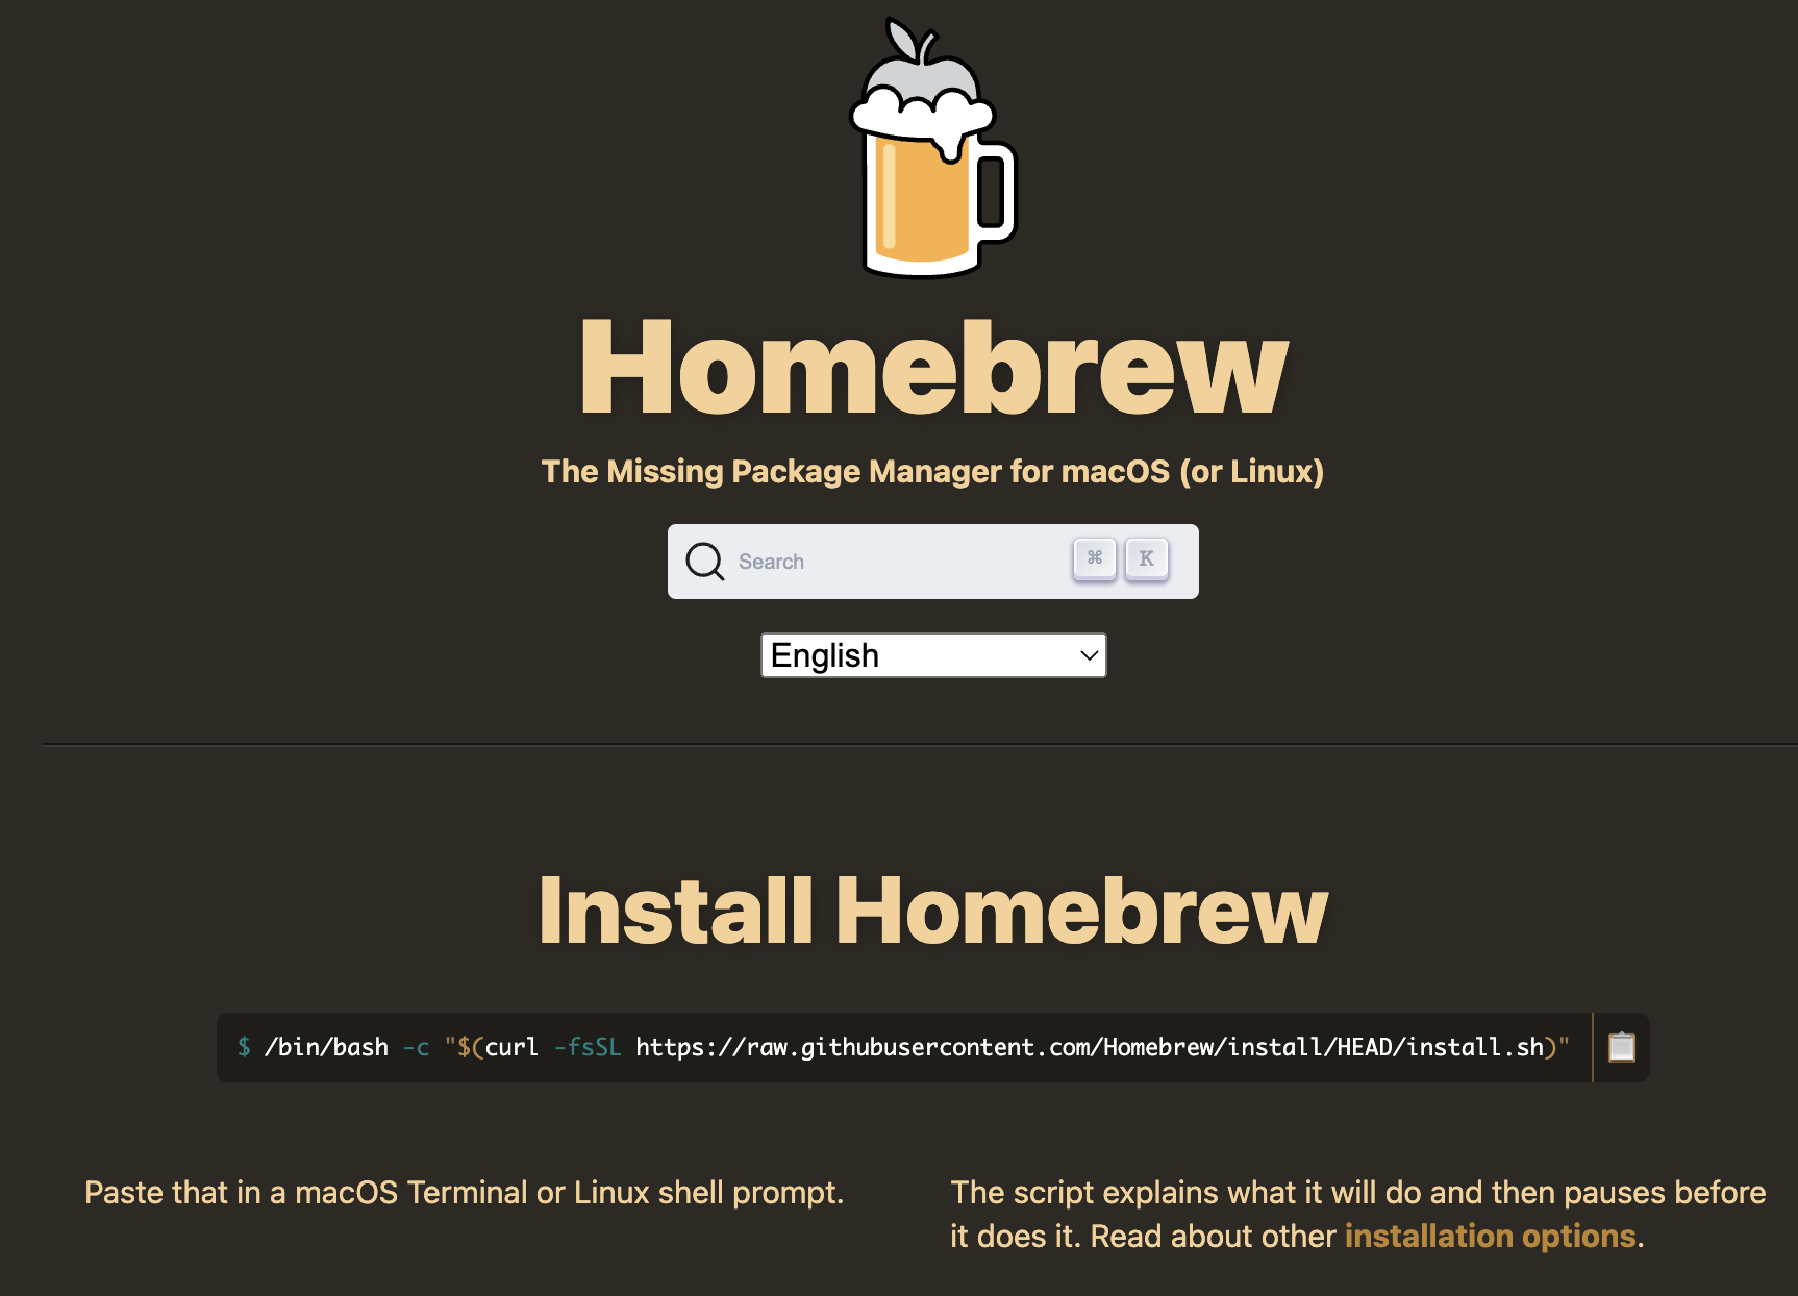
\includegraphics[width=\linewidth]{external/brew_homepage.pdf}
\end{image}%
\tcblower
\end{figureptx}%
\footnotetext[14]{\nolinkurl{brew.sh}\label{fn-brew-homepage-a-b}}%
Once you paste in that command, press \kbd{Enter} and follow the instructions on installation. Don't worry about what each part does (to be honest, I'm not entirely sure either). It is safe and trustworthy (I did it on my computer).%
\item{}Now, use Homebrew to install Git. Simply type in \mono{brew install git} at the terminal and press \kbd{Enter}.%
\end{enumerate}
And that's it!%
\end{paragraphs}%
\begin{paragraphs}{GitHub.}{paragraphs-materials-mac-e}%
You will also need a GitHub account. Since this is an extensive topic, this is covered in \hyperref[subsection-hub-account]{Subsection~{\xreffont\ref{subsection-hub-account}}}.%
\end{paragraphs}%
\end{preface}
%
%
\typeout{************************************************}
\typeout{Preface  Materials: Linux}
\typeout{************************************************}
%
\begin{preface}{Preface}{Materials: Linux}{}{Materials: Linux}{}{}{preface-materials-linux}
As this book was written on the assumption that you have no experience with Git or the command line, it also assumes you do not have necessary materials (software). Downloads will differ slightly depending on it you have a Mac or a \initialism{PC} and if you are running Linux. The following will provide necessary materials to use this book as well as links and some relevant instructions \emph{for those who are using Linux}.%
\par
Please note that I have no experience with using Linux. These instructions will likely be superficial and without detail. I simply provide you with links; I am currently not able to provide information on how to install software correctly.%
\begin{paragraphs}{A Text Editor.}{paragraphs-materials-linux-d}%
In order to edit files as demonstrated in this book, you will need a text editor outside of the basic default editor. Any editor will work such as \href{https://www.sublimetext.com/download}{Sublime Text}\footnote{\nolinkurl{sublimetext.com/download}\label{fn-materials-linux-d-b-b}} which has a Linux download.%
\par
If you are already familiar with an editor or if you like a particular one, use it! However, I personally prefer \href{https://code.visualstudio.com/Download}{Visual Studio (VS) Code}\footnote{\nolinkurl{code.visualstudio.com/Download}\label{fn-materials-linux-d-c-b}} which can be downloaded at the previous link (there is a Linux download). Throughout this book, I will refer to \initialism{VS} Code with some guidelines on how to find certain features. Should you decide to use another editor, it is up to you to learn how to use it. If you are a beginner with Git and the command line, I would stick with \initialism{VS} Code although as you gain experience you might think about switching to Sublime Text.%
\end{paragraphs}%
\begin{paragraphs}{Git.}{paragraphs-materials-linux-e}%
To use Git, you need to download and install it on your computer. You already have a command line, you just need to make sure that you have Git. Depending on your computer and where you got it, you may actually already have Git (for instance, university laptops). You can install Git for Linux from the many options \href{https://git-scm.com/download/linux}{at the GitHub download page}\footnote{\nolinkurl{git-scm.com/download/linux}\label{fn-materials-linux-e-b-b}}.%
\end{paragraphs}%
\begin{paragraphs}{GitHub.}{paragraphs-materials-linux-f}%
You will also need a GitHub account. Since this is an extensive topic, this is covered in \hyperref[subsection-hub-account]{Subsection~{\xreffont\ref{subsection-hub-account}}}.%
\end{paragraphs}%
\end{preface}
%% begin: table of contents
%% Adjust Table of Contents
\setcounter{tocdepth}{0}
\renewcommand*\contentsname{Contents}
\tableofcontents
%% end:   table of contents
\mainmatter
%
%
\typeout{************************************************}
\typeout{Part I Introductory Information}
\typeout{************************************************}
%
\begin{partptx}{Part}{Introductory Information}{}{Introductory Information}{}{}{part-part-intro}
\renewcommand*{\partname}{Part}
 %
%
\typeout{************************************************}
\typeout{Chapter 1 Computer Basics}
\typeout{************************************************}
%
\begin{chapterptx}{Chapter}{Computer Basics}{}{Computer Basics}{}{}{chapter-C_basics}
\renewcommand*{\chaptername}{Chapter}
\begin{introduction}{}%
For those who do not have a lot of experience with computers, start here for an introduction into certain computer basics. This book assumes that you are familiar with the content in this chapter so take some time to browse it. Don't worry, I don't assume you know anything about the ``command line'' (this will be introduced in \hyperref[section-S_whatiscommline]{Section~{\xreffont\ref{section-S_whatiscommline}}}).%
\par
However, for the content of this book to make sense, a few basics must be covered, such as proper file naming and a knowledge of common file extensions. Taking the time to read this chapter \emph{will} pay off in the long run and will make using the command line and Git simpler (and we love simplicity, espeically with computers!).%
\end{introduction}%
%
%
\typeout{************************************************}
\typeout{Section 1.1 File and Folder Names}
\typeout{************************************************}
%
\begin{sectionptx}{Section}{File and Folder Names}{}{File and Folder Names}{}{}{section-S_filenames}
\index{file names}%
\index{folder names}%
\begin{introduction}{}%
Take a minute and look at some of the files and folders on your computer. What do the names look like?%
\par
Sorry, that probably wasn't very clear. Specifically, I want you to see if there are \emph{spaces} in your file and folder names. My guess is probably! Mine certainly had spaces before I learned more about computers and got involved in Git and the command line.%
\par
Take another look at some files\slash{}folders. What is your ``capitalization scheme''? Is there a pattern? Do you name your files by what they contain? Do you have dates in your files? Do you have a group of files with something like ``File First Draft'', ``File Second Draft'', ``File, revisions from colleague'', etc.? All of these can be problematic for computers and even more so for humans interacting with computers.%
\par
The following chunks go through my opinions on file naming conventions. But that's what they are: opinions. Suggestions. Following them will make your life easier later on. But by all means, go ahead and ignore me and decide for yourself later if you want to make a change. I probably won't pop up in your home and check your file names. Try not to get too lost with these; an extensive example will be provided at the end of the section.%
\end{introduction}%
%
%
\typeout{************************************************}
\typeout{Subsection 1.1.1 Naming Conventions}
\typeout{************************************************}
%
\begin{subsectionptx}{Subsection}{Naming Conventions}{}{Naming Conventions}{}{}{subsection-SS_namingconventions}
\begin{paragraphs}{File Names With Revisions.}{paragraphs-namesrevisions}%
\index{file names!with revisions}%
\index{version control}%
You might be familiar with this situation: You write one draft, get feedback, save a second draft as a new file, get feedback again, and finally make a new file with a final draft. Then, you decide to make modifications to that final draft which is saved as a new file, etc., etc.This is great until you realize that now you have way too many files for a single document. How do you know which one is real final draft? What if you open the wrong one and start editing? Now you have to edit all of the files to make them match.%
\par
Sure, a computer can handle that many files and doesn't really care how many drafts or revisions you have. But more files take up more storage space and increases the chances of confusing you! How on earth can we solve this problem? It's not like there's a magic software that can keep track of all of our changes in a single file.%
\par
Ah, but there is! This magic software is called Git. Git specializes in \terminology{version control} which means that you do not have to worry about twelve drafts. Git keeps track of your revision history for you. If you are familiar with Google Docs, Git is very similar. Docs saves your changes and makes it easy to revert back to an old version if you change your mind on anything.%
\par
For now, don't worry about Git; we will get there in \hyperref[chapter-C_gitsolo]{Chapter~{\xreffont\ref{chapter-C_gitsolo}}}. Just know that after reading this book, you won't have to worry about excess drafts and should never have to save so many drafts again.%
\end{paragraphs}%
\begin{paragraphs}{File Names With Dates.}{paragraphs-namesdates}%
\index{file names!with dates}%
Ok, this isn't entirely problematic. But I never understood why dates in file names had to be so specific. Having years makes sense, maybe months. But days? Times? Seconds? Once you start getting that specific with dates and times, you run into the same issue as in \hyperlink{paragraphs-namesrevisions}{File Names With Revisions}. Dates and times just make your file names incredibly long, hard to read, and hard to use in the command line. Please try to avoid dates, other than years, perhaps.%
\end{paragraphs}%
\begin{paragraphs}{Descriptive File Names.}{paragraphs-namesdescriptive}%
\index{file names!descriptive}%
\index{file names!shortening tricks}%
File names should be descriptive! Furthermore, they should describe \emph{what the file actually contains\slash{}is about} and not some random name. Probably most of your files are descriptive? That's great! But what's the catch? File names should also be short. Short, sweet, to the point, and also descriptive.%
\par
That's pretty tricky, you might say. Sure, I respond, but you can take advantage of abbreviations and word-shortening tricks. For instance, suppose I had a file name like this:%
\begin{quote}%
Chapters3\textunderscore{}4\textunderscore{}Overview of Sampling and Simple Random Sampling (SRS).pdf%
\end{quote}
This is clearly descriptive. We know exactly what this PDF is about: it refers to chapters 3 and 4 of a textbook which is about sampling in general and digs into simple random sampling. But wow, it's really long. On my computer, it shows up as%
\begin{quote}%
Chapters3\textunderscore{}4\textunderscore{}Overview of\textellipsis{}SRS).pdf%
\end{quote}
Now do you know what this file contains? I don't. Yes, it's on chapters 3 and 4 but we are left hanging as to what the chapters are an overview of! Moreover, what does the random ``SRS'' mean at the end?%
\par
If it were me, I would rather name this file (based on the conventions discussed so far)%
\begin{quote}%
Ch3\textunderscore{}4\textunderscore{}Sampling and SRS.pdf%
\end{quote}
Wow! So much shorter. Do you still have an idea of what the file contains? Hopefully! ``Ch'' is usually accepted as an abbreviation for ``Chapter'' so it is clear that this file is over chapters 3 and 4. The subject of these chapters is sampling and simple random sampling (``SRS'' is a widely-used abbreviation in statistics for simple random sampling).%
\begin{assemblage}{Assemblage}{File Naming Trick.}{assemblage-namesdescriptive-m}%
An easy way to shorten file names is to remove the vowels from words. The human brain is incredible in that it can determine what a word should be based on a small amount of context. Assuming the file above was in a folder pertaining to statistics, I could shorten it even more:%
\begin{quote}%
Ch3\textunderscore{}4\textunderscore{}Smplng and SRS.pdf%
\end{quote}
And we still know what it's about!%
\par
A quick word of caution. Take care not to over-abbreviate. It may not be necessary to abbreviate every word. For instance, I wouldn't change ``you'' to ``y'' or ``gate'' to ``gt''. You may be confused later: does ``gt'' mean ``gate'', ``git'', ``get'', ``gut'', ``agate'', etc., etc.?%
\end{assemblage}
Summary: keep your file names short and to the point. Describe what the file is (I wouldn't name the file above ``bananas.pdf''!).%
\end{paragraphs}%
\begin{paragraphs}{File Names With Spaces.}{paragraphs-namesspaces}%
\index{file names!with spaces}%
If you only follow one convention in this section, this would be the one. This the most important for working with the command line. Spaces in file names increase the amount of typing you have to do and make it more difficult to understand what's going on on the command line.%
\par
For instance, suppose I wanted to open the file we discussed earlier. On the command line, I would open the file like this (don't worry about the commands, just notice what it looks like):%
\begin{quote}%
\mono{open \textquotesingle{}Chapters3\_4\_Overview of Sampling and Simple Random Sampling (SRS).pdf\textquotesingle{}}%
\end{quote}
I could also do it like this:%
\begin{quote}%
\mono{open Chapters3\_4\_Overview\textbackslash{} of\textbackslash{} Sampling\textbackslash{} and\textbackslash{} Simple\textbackslash{} Random\textbackslash{} Sampling\textbackslash{} (SRS).pdf}%
\end{quote}
First, notice how long these titles are. That's a lot to type! What you should really notice is that in the first example, the file is surrounded in quotes and in the second, there are a bunch of backslashes. For each file name with spaces, you have to either remember to enclose the entire name in quotes or to take the time to put a backslash before every space. It may not seem like too much of a hassle, but you will get annoyed with it pretty quickly. It also can cause setbacks inside code editors when you want to import or export files with spaces.%
\par
So what do we replace the spaces with?%
\begin{note}{Note}{Alternative Naming Options.}{note-filenamecases}%
\index{cases}%
\index{file names}%
\index{naming|see{file names}}%
Most computer programmers name their files using \terminology{cases}. There are five main cases:%
\begin{descriptionlist}
\begin{dlimedium}{snake\textunderscore{}case}{li-filenamecases-e-b-a}%
no capital letters, spaces are replaced with underscores (\textunderscore{})%
\end{dlimedium}%
\begin{dlimedium}{kebab-case}{li-filenamecases-e-b-b}%
no capital letters, spaces are replaced with hyphens (-)%
\end{dlimedium}%
\begin{dlimedium}{camelCase}{li-filenamecases-e-b-c}%
first word is lowercase, all consequent words are capitalized; spaces are removed%
\end{dlimedium}%
\begin{dlimedium}{PascalCase}{li-filenamecases-e-b-d}%
every word is capitalized, spaces are removed%
\end{dlimedium}%
\begin{dlimedium}{UPPER\textunderscore{}CASE\textunderscore{} SNAKE\textunderscore{}CASE}{li-filenamecases-e-b-e}%
every letter is capitalized, spaces are replaced with underscores (\textunderscore{})%
\end{dlimedium}%
\end{descriptionlist}
See a \href{https://chaseadams.io/posts/most-common-programming-case-types/}{Most Common Programming Case Types blog post}\footnotemark{} to get more details on these cases.%
\end{note}
\footnotetext[18]{\nolinkurl{chaseadams.io/posts/most-common-programming-case-types/}\label{fn-filenamecases-e-d}}%
Personally, I use snake\textunderscore{}case for file names and kebab-case for folder names, just to help me keep them separate and still easy to read. I also tend to name my files and folders with lowercase letters if I can.%
\par
Using the shortened file name above, I would use the following as my file name:%
\begin{quote}%
ch3\textunderscore{}4\textunderscore{}smplng\textunderscore{}srs.pdf%
\end{quote}
Note that I got rid of the ``and''. Cases are useful in that they make it easy to remove articles and prepositions which in turn helps us keep file names nice and short.%
\par
It is also important to keep your file names consistent. If I had another file about chapter 5 of this textbook which is about cluster sampling, let's say, I would want to name it something like%
\begin{quote}%
ch5\textunderscore{}clstr\textunderscore{}smplng.pdf%
\end{quote}
Notice that the structure is the same as before: first I have ``ch5'' to represent the chapter number, then I describe the chapter with ``clstr\textunderscore{}smplng''. Like before, I use snake\textunderscore{}case and I made sure to use the same abbreviation for ``sampling'' as I did before. Consistency is key for our own sanity and so we can quickly scan for the file we need.%
\par
It's worth repeating once again. File names should not contain spaces. Files about related content should have a similar naming scheme.%
\par
Sorry, once more. This time, I'm going to yell. \alert{File names should not contain spaces.}%
\end{paragraphs}%
\begin{paragraphs}{A Quick Note on Folder Names.}{paragraphs-SS_namingconventions-f}%
\index{folder names}%
\index{directory names|see{folder names}}%
Folder names should also follow all of the conventions above. This is a lot harder to get used to. I still feel like I'm breaking the Human Code of Folder Names everytime I ignore spaces and capital letters. For whatever reason, I'm fine with file names, but folder names just don't feel right.%
\par
But too bad for me! I name my folders according to the conventions anyways. And you should too. (As I mentioned earlier, I use snake\textunderscore{}case for files and kebab-case for folders. You might consider doing so as well; they are the two most popular cases.)%
\end{paragraphs}%
\end{subsectionptx}
%
%
\typeout{************************************************}
\typeout{Subsection 1.1.2 Exploring File and Folder Naming Techniques}
\typeout{************************************************}
%
\begin{subsectionptx}{Subsection}{Exploring File and Folder Naming Techniques}{}{Exploring File and Folder Naming Techniques}{}{}{subsection-SS_practicenaming}
There were a lot of words in \hyperref[subsection-SS_namingconventions]{Subsection~{\xreffont\ref{subsection-SS_namingconventions}}}. Let's make sense of them here with an extensive example. There will be some questions throughout the way. I encourage you to think about them and make sure you have understood the naming conventions above.%
\begin{activity}{Activity}{Folder Naming.}{activity-taylorswiftfolders}%
\index{folder names}%
Suppose you work for Taylor Swift (wouldn't that be cool!). She is super busy right now recording albums, writing songs, spending time with family and friends, and making TikToks and needs your help. She has all of her songs saved on her computer in folders which are divided up by one album per folder. She has asked you to help her rename her folders so that she still knows what each folder is, but follows proper naming conventions. Use your knowledge from above to help Taylor out.%
\par
Following is a list of her current folder names:%
\begin{multicols}{2}
\begin{itemize}[label=\textbullet]
\item{}Taylor Swift%
\item{}Taylor Swift (Deluxe)%
\item{}Live From Clear Channel Stripped 2008%
\item{}Fearless%
\item{}Fearless (Platinum Edition)%
\item{}The Taylor Swift Holiday Collection%
\item{}Speak Now%
\item{}Speak Now (Deluxe Edition)%
\item{}Speak Now World Tour Live%
\item{}Red%
\item{}Red (Deluxe Edition)%
\item{}1989%
\item{}1989 (Deluxe Edition)%
\item{}reputation%
\item{}Lover%
\item{}folklore%
\item{}folklore (deluxe edtion)%
\item{}folklore: the long pond studio sessions (from the Disney+ special) [deluxe edition]%
\item{}evermore%
\item{}evermore (deluxe version)%
\item{}Fearless (Taylor's Version)%
\item{}Red (Taylor's Version)%
\item{}Midnights%
\item{}Midnights (3am Edition)%
\item{}Midnights (The Til Dawn Edition)%
\item{}Speak Now (Taylor's Version)%
\item{}Unreleased Music%
\item{}Singles%
\end{itemize}
\end{multicols}
%
\par
Wow! That's a lot of albums! Complete the following tasks to make Taylor's life a little easier for the future.%
\par
Please note that the answers to many of these exercises will vary depending on personal preferences. I will give answers depending on how I might approach the problem; they are certainly not the only answer you could have given.%
\begin{enumerate}[font=\bfseries,label=(\alph*),ref=\alph*]%
\item{}Before we trying fixing a problem, let's figure out what the problem is. What do you notice about these folder names? What about them is ``incorrect''?%
\item\label{task-taylorswiftgroups}Ok, we've identified a problem. How can we go about deciding what to do about it? You may already have some ideas, but stick with me here. Let's not just dive in and start removing spaces and shortening folder names. Instead, let's make a plan.%
\par
Identify some naming patterns. Are there any album names that are similar? Can you form any groups of names?%
\item{}I am going to continue with the groups in the solution to \hyperref[task-taylorswiftgroups]{Task~{\xreffont\ref{activity-taylorswiftfolders}}.{\xreffont\ref{task-taylorswiftgroups}}}. Feel free to branch off with your own groups or stick with me.%
\par
Now that we have groups, we can figure out how to name one of each group, then apply that naming style to all names in the group. Start with the standard albums, such as ``Taylor Swift''. How can you change this name to stick with the conventions discussed above?%
\item{}Apply the naming to scheme to all folders with ``regular'' album titles.%
\item{}Continue with the deluxe group. Identify patterns, change one name, then apply those changes to all the names in the group. Use your best judgement, but don't stress about the ``perfect'' name.%
\item{}Continue with the live group. Identify patterns, change one name, then apply those changes to all the names in the group. Use your best judgement, but don't stress about the ``perfect'' name.%
\item{}Continue with the Taylor's Version group. Identify patterns, change one name, then apply those changes to all the names in the group. Use your best judgement, but don't stress about the ``perfect'' name.%
\item{}Continue with the other group. Identify patterns, change one name, then apply those changes to all the names in the group. Use your best judgement, but don't stress about the ``perfect'' name.%
\end{enumerate}%
I think that's all of them! That may have seemed like a lot of work but I hope it was worthwhile. It should now be much easier for Taylor to navigate her folders and quickly know that album they contain.%
\end{activity}%
If you feel like you have a good grasp of naming systems, feel free to skip \hyperref[activity-taylorswiftfiles]{Activity~{\xreffont\ref{activity-taylorswiftfiles}}}. If not, let's explore file naming a little further. In \hyperref[activity-taylorswiftfolders]{Activity~{\xreffont\ref{activity-taylorswiftfolders}}}, we focused on Taylor's folder names and since you helped her there, she is asking for your guidance with her file names as well.%
\begin{activity}{Activity}{File Naming.}{activity-taylorswiftfiles}%
\index{file names}%
We will focus on the folder that I renamed to be \mono{speak-now-dlx}. A list of her current file names for these tracks follow. I should note that it is often helpful to prefix song names with their track position so that they stay in order when in a folder. We won't remove those numbers. Also, ``.wav'' indicates that the song is a WAV file (see \hyperref[section-S_fileextensions]{Section~{\xreffont\ref{section-S_fileextensions}}} for more). We should not remove these either as this could result in file loss or corruption.%
\begin{multicols}{2}
\begin{itemize}[label=\textbullet]
\item{}01 Mine.wav%
\item{}02 Sparks Fly.wav%
\item{}03 Back To December.wav%
\item{}04 Speak Now.wav%
\item{}05 Dear John.wav%
\item{}06 Mean.wav%
\item{}07 The Story Of Us.wav%
\item{}08 Never Grow Up.wav%
\item{}09 Enchanted.wav%
\item{}10 Better Than Revenge.wav%
\item{}11 Innocent.wav%
\item{}12 Haunted.wav%
\item{}13 Last Kiss.wav%
\item{}14 Long Live.wav%
\item{}15 Ours.wav%
\item{}16 If This Was A Movie.wav%
\item{}17 Superman.wav%
\item{}18 Back To December (Acoustic).wav%
\item{}19 Haunted (Acoustic Version).wav%
\item{}20 Mine (POP Mix).wav%
\end{itemize}
\end{multicols}
%
\par
Like before, complete the following tasks to make Taylor's life a little easier for the future.%
\par
Again note that the answers to many of these exercises will vary depending on personal preferences. I will give answers depending on how I might approach the problem; these are not the only correct responses.%
\begin{enumerate}[font=\bfseries,label=(\alph*),ref=\alph*]%
\item{}Before we trying fixing a problem, let's figure out what the problem is. What do you notice about these file names? What about them is ``incorrect''?%
\item\label{task-taylorswiftgroups2}Ok, we've identified a problem. How can we go about deciding what to do about it? You may already have some ideas, but stick with me here. Let's not just dive in and start removing spaces and shortening file names. Instead, let's make a plan.%
\par
Identify some naming patterns. Are there any track names that are similar? Can you form any groups of names?%
\item{}I am going to continue with the groups in the solution to \hyperref[task-taylorswiftgroups2]{Task~{\xreffont\ref{activity-taylorswiftfiles}}.{\xreffont\ref{task-taylorswiftgroups2}}}. Feel free to branch off with your own groups or stick with me.%
\par
Now that we have groups, we can figure out how to name one of each group, then apply that naming style to all names in the group. Start with the ``regular'' tracks. How can you change these names to stick with the conventions discussed above?%
\item{}Apply the naming to scheme to all the acoustic tracks.%
\item{}Apply the naming to scheme to all the last track.%
\end{enumerate}%
And that's it! If you would like more practice, look up the track listing for her other albums and repeat this activity. It would be a great activity in consistency; for example, for the tracks on the Taylor's Version albums, you would want to use the same naming scheme as in the folders. For me, I would say \mono{02\_red\_tv.wav} for ``Red (Taylor's Version)'' and to any acoustic tracks, I would append \mono{\_acoust}.%
\end{activity}%
\end{subsectionptx}
\end{sectionptx}
%
%
\typeout{************************************************}
\typeout{Section 1.2 File Extensions}
\typeout{************************************************}
%
\begin{sectionptx}{Section}{File Extensions}{}{File Extensions}{}{}{section-S_fileextensions}
\index{file extensions}%
\begin{introduction}{}%
There are many different types of files. At the very basics, we have images, videos, documents, and songs, but there are so many more. Even within each of those categories, there are numerous types. You may be familiar with a PDF and a Word Document. Both of those could be classified as ``documents'', but are interacted with very differently. Whether you are an advanced computer programmer or someone who uses a computer for every-day purposes, an understanding of file extensions is essential. \terminology{File extensions} help us understand what type of file we are working with and give us an idea of how we can interact with that file. The following chunks give common (and some not so common) extensions for various categories. Refer back to this section often, especially if you find yourself forgetting what a file is.%
\par
Hint: \kbd{Control} + \kbd{F} or \kbd{Command} + \kbd{F} work well on this page.%
\end{introduction}%
%
%
\typeout{************************************************}
\typeout{Subsection 1.2.1 Images}
\typeout{************************************************}
%
\begin{subsectionptx}{Subsection}{Images}{}{Images}{}{}{subsection-extensions-images}
\index{file extensions!images}%
Why would we need more than on extension for an image? A photo is a photo, right? Wrong. Each of the file extensions have unique aspects and features. For instance, the Apple \mono{.heic} file often takes up less storage space. However, not all programs can open them. The \href{https://guides.lib.umich.edu/c.php?g=282942\&p=1885348}{University of Michigan}\footnote{\nolinkurl{guides.lib.umich.edu/c.php?g=282942\&p=1885348}\label{fn-extensions-images-c-c}} and \href{https://kinsta.com/blog/image-file-types/}{Kinsta}\footnote{\nolinkurl{kinsta.com/blog/image-file-types/}\label{fn-extensions-images-c-e}} have great guides on the differences between some image file extensions. The table here just lists the extensions and what they are, not the details on their use.%
\begin{tableptx}{Table}{\textbf{Image File Extensions}}{table-tbl-image-extensions}{}%
\centering%
{\tabularfont%
\begin{tabular}{cc}
{\bfseries{}Extension}&{\bfseries{}File Type}\tabularnewline[0pt]
\mono{.jpg} or \mono{.jpeg}&Joint Photographic Experts Groups image\tabularnewline[0pt]
\mono{.png}&Portable Network Graphics image\tabularnewline[0pt]
\mono{.svg}&Scalable Vector Graphics image\tabularnewline[0pt]
\mono{.gif}&A looped image\slash{}video blend\tabularnewline[0pt]
\mono{.eps}&Encapsulated PostScript (vector) image\tabularnewline[0pt]
\mono{.bmp}&Bitmap image\tabularnewline[0pt]
\mono{.tif} or \mono{.tiff}&Tagged Image File Format\tabularnewline[0pt]
\mono{.raw}&Raw image (usually from a camera)\tabularnewline[0pt]
\mono{.HEIF}&High Efficiency Image File\tabularnewline[0pt]
\mono{.HEIC}&High Efficiency Image Container (Apple)\tabularnewline[0pt]
\mono{.psd}&Adobe Photoshop\tabularnewline[0pt]
\mono{.ai}&Adobe Illustrator
\end{tabular}
}%
\end{tableptx}%
\end{subsectionptx}
%
%
\typeout{************************************************}
\typeout{Subsection 1.2.2 Videos}
\typeout{************************************************}
%
\begin{subsectionptx}{Subsection}{Videos}{}{Videos}{}{}{subsection-extensions-videos}
\index{file extensions!videos}%
\href{https://www.adobe.com/creativecloud/video/discover/best-video-format.html}{Adobe}\footnote{\nolinkurl{adobe.com/creativecloud/video/discover/best-video-format.html}\label{fn-extensions-videos-c-b}} has a great guide on the differences between some video file extensions. The table here just lists the extensions and what they are, not the details on their use.%
\begin{tableptx}{Table}{\textbf{Video File Extensions}}{table-tbl-video-extensions}{}%
\centering%
{\tabularfont%
\begin{tabular}{cc}
{\bfseries{}Extension}&{\bfseries{}File Type}\tabularnewline[0pt]
\mono{.mp4}&MPEG-4\tabularnewline[0pt]
\mono{.mov}&QuickTime Movie\tabularnewline[0pt]
\mono{.wmv}&Windows Media Viewer\tabularnewline[0pt]
\mono{.avi}&Audio Video Interleave\tabularnewline[0pt]
\mono{.prproj}&Adobe Premiere Pro Project\tabularnewline[0pt]
\mono{.aep}&Adobe After Effect Project\tabularnewline[0pt]
\mono{.fcp}&Apple Final Cut Project\tabularnewline[0pt]
\mono{.camproj}&Camtasia Project\tabularnewline[0pt]
\mono{.m4v}&iTunes Movie File
\end{tabular}
}%
\end{tableptx}%
\end{subsectionptx}
%
%
\typeout{************************************************}
\typeout{Subsection 1.2.3 Documents}
\typeout{************************************************}
%
\begin{subsectionptx}{Subsection}{Documents}{}{Documents}{}{}{subsection-extensions-docs}
\index{file extensions!documents}%
There are many different file extensions that refer to documents. Many of them you will never encounter. Only the main file types are listed here. \href{https://blog.filestack.com/thoughts-and-knowledge/document-file-extensions-list/}{File Stack}\footnote{\nolinkurl{blog.filestack.com/thoughts-and-knowledge/document-file-extensions-list/}\label{fn-extensions-docs-c-b}} has a good explanation on some of the file types here.%
\begin{center}%
{\tabularfont%
\begin{tabular}{cc}
{\bfseries{}Extension}&{\bfseries{}File Type}\tabularnewline[0pt]
\mono{.doc} or \mono{.docx}&Microsoft Word Document\tabularnewline[0pt]
\mono{.xsl} or \mono{.xslx}&Microsoft Excel Spreadsheet\tabularnewline[0pt]
\mono{.ppt} or \mono{.pptx}&Microsoft PowerPoint Presentation\tabularnewline[0pt]
\mono{.pages}&Apple Document\tabularnewline[0pt]
\mono{.key}&Apple Keynote Presentation\tabularnewline[0pt]
\mono{.numbers}&Apple Numbers Spreadsheet\tabularnewline[0pt]
\mono{.pdf}&Adobe Portable Document Format\tabularnewline[0pt]
\mono{.rtf}&Rich Text Format Document\tabularnewline[0pt]
\mono{.txt}&Plain Text Document\tabularnewline[0pt]
\mono{.log}&Text Log File (often records messages)\tabularnewline[0pt]
\mono{.md}&MarkDown Document\tabularnewline[0pt]
\mono{.Rmd}&MarkDown Document for use in R
\end{tabular}
}%
\end{center}%
Note: technically, \mono{.html} and \mono{.xml} are considered document-type files. I am choosing to place them under coding-type files instead.%
\end{subsectionptx}
%
%
\typeout{************************************************}
\typeout{Subsection 1.2.4 Audio}
\typeout{************************************************}
%
\begin{subsectionptx}{Subsection}{Audio}{}{Audio}{}{}{subsection-extensions-audio}
\index{file extensions!audio}%
\href{https://www.makeuseof.com/tag/audio-file-format-right-needs/}{makeuseof.com}\footnote{\nolinkurl{makeuseof.com/tag/audio-file-format-right-needs/}\label{fn-extensions-audio-c-b}} has great descriptions of the most common audio file types.%
\begin{center}%
{\tabularfont%
\begin{tabular}{cc}
{\bfseries{}Extension}&{\bfseries{}File Type}\tabularnewline[0pt]
\mono{.mp3}&MPEG Layer 3 (lossy compression)\tabularnewline[0pt]
\mono{.wav}&Waveform Audio Format (uncompressed)\tabularnewline[0pt]
\mono{.aiff}&Audio Interchange File Format (uncompressed)\tabularnewline[0pt]
\mono{.aac}&Advanced Audio Coding (lossy compression)\tabularnewline[0pt]
\mono{.wma}&Windows Media Audio (lossy compression)\tabularnewline[0pt]
\mono{.flac}&Free Lossless Audio Codec (lossless compression)\tabularnewline[0pt]
\mono{.aa} or \mono{.aax}&Audible Audio File\tabularnewline[0pt]
\mono{.m4a}&Audio-Only MPEG-4 (iTunes)\tabularnewline[0pt]
\mono{.midi}&MIDI File
\end{tabular}
}%
\end{center}%
\end{subsectionptx}
%
%
\typeout{************************************************}
\typeout{Subsection 1.2.5 Coding and Programming}
\typeout{************************************************}
%
\begin{subsectionptx}{Subsection}{Coding and Programming}{}{Coding and Programming}{}{}{subsection-extensions-coding}
\index{file extensions!coding}%
There is a plethora of programming languages, software, and interfaces and each of them uses a different file extension.%
\begin{center}%
{\tabularfont%
\begin{tabular}{cc}
{\bfseries{}Extension}&{\bfseries{}File Type}\tabularnewline[0pt]
\mono{.R}&R Script\tabularnewline[0pt]
\mono{.py}&Python Script\tabularnewline[0pt]
\mono{.ipynb}&Jupyter Notebook\tabularnewline[0pt]
\mono{.html}&HyperText Markup Language\tabularnewline[0pt]
\mono{.css}&Cascading Style Sheets\tabularnewline[0pt]
\mono{.js}&Javascript\tabularnewline[0pt]
\mono{.sas}&SAS Script\tabularnewline[0pt]
\mono{.xml}&eXtensible Markup Language\tabularnewline[0pt]
\mono{.xslt}&eXtensible Style Sheet Transformations\tabularnewline[0pt]
\mono{.ptx}&PreTeXt Markup File\tabularnewline[0pt]
\mono{.tex}&LaTeX Document (typically for mathematics)\tabularnewline[0pt]
\mono{.c}&C and C++ File\tabularnewline[0pt]
\mono{.cpp}&C++ File\tabularnewline[0pt]
\mono{.java}&Java Source\tabularnewline[0pt]
\mono{.swift}&Swift Code File\tabularnewline[0pt]
\mono{.vb}&Visual Basic File\tabularnewline[0pt]
\mono{.vbs}&Visual Basic Script
\end{tabular}
}%
\end{center}%
\end{subsectionptx}
%
%
\typeout{************************************************}
\typeout{Subsection 1.2.6 Data}
\typeout{************************************************}
%
\begin{subsectionptx}{Subsection}{Data}{}{Data}{}{}{subsection-extensions-data}
\index{file extensions!data}%
Many of these extensions also belong in \hyperref[subsection-extensions-docs]{Subsection~{\xreffont\ref{subsection-extensions-docs}}} but are related enough to merit another subsection.%
\begin{center}%
{\tabularfont%
\begin{tabular}{cc}
{\bfseries{}Extension}&{\bfseries{}File Type}\tabularnewline[0pt]
\mono{.csv}&Comma Separated Values\tabularnewline[0pt]
\mono{.tsv} or \mono{.tab}&Tab Separated Values\tabularnewline[0pt]
\mono{.json}&JavaScript Object Notation\tabularnewline[0pt]
\mono{.csv}&Comma Separated Values\tabularnewline[0pt]
\mono{.tsv}&Tab Separated Values\tabularnewline[0pt]
\mono{.rds}&Single R Object\tabularnewline[0pt]
\mono{.RData}&Multiple R Objects\tabularnewline[0pt]
\mono{.sas7bdat}&SAS Data File
\end{tabular}
}%
\end{center}%
\end{subsectionptx}
%
%
\typeout{************************************************}
\typeout{Subsection 1.2.7 Other File Exensions}
\typeout{************************************************}
%
\begin{subsectionptx}{Subsection}{Other File Exensions}{}{Other File Exensions}{}{}{subsection-extensions-other}
\index{file extensions!other}%
\begin{center}%
{\tabularfont%
\begin{tabular}{cc}
{\bfseries{}Extension}&{\bfseries{}File Type}\tabularnewline[0pt]
\mono{.band}&Apple GarageBand File\tabularnewline[0pt]
\mono{.logicx}&Apple Logic Pro File\tabularnewline[0pt]
\mono{.exe}&Windows Executable File\tabularnewline[0pt]
\mono{.zip}&Compressed Files\tabularnewline[0pt]
\mono{.tar.gz}&Collection of (archived) files\tabularnewline[0pt]
\mono{.app}&Mac Application\tabularnewline[0pt]
\mono{.dmg}&Mac Disc Image (executable file)\tabularnewline[0pt]
\mono{.pkg}&Package of Software or Files\tabularnewline[0pt]
\mono{.otf}&Open Type Font\tabularnewline[0pt]
\mono{.ttf}&TrueType Font
\end{tabular}
}%
\end{center}%
\end{subsectionptx}
\end{sectionptx}
%
%
\typeout{************************************************}
\typeout{Section 1.3 File Paths}
\typeout{************************************************}
%
\begin{sectionptx}{Section}{File Paths}{}{File Paths}{}{}{section-S_filepaths}
\index{file paths}%
\index{paths|see{file paths}}%
\begin{introduction}{}%
Imagine that I bring you to the edge of a forest, an immense, thick, unexplored forest. When we get there, I tell you that somewhere in that forest lays a chest of pure diamonds, put there 1000 years ago. Then I give you a task: I need you to go find that chest for me (yes, you get a portion of the loot).%
\par
Think about how you might go about this task. The forest is unexplored; we only know that the chest exists inside. Where will you look first? Where will you enter? How will you keep track of where you've been? If you find it, how will you get back? There are many issues preventing you from doing your task efficiently. Sure, you could get lucky and the chest might be only 50 feet from the edge. But maybe it's 3000 feet away (or more!).%
\par
Think of your computer like the forest. If I ask my computer to open a file called \mono{poem.pdf}, how will it know where to look for that file? Like you in the forest, it wouldn't even know where to start. Likewise, what if I had two files named \mono{poem.pdf} in different folders? What if I had two files named \mono{poem.pdf} in the same folder? How would it know which one to grab? It wouldn't! It's like me telling you there are two identical chests of diamonds in the forest and I want you to bring me the one I am thinking about. But you don't know the one I am thinking about.%
\par
This situation necessitates file paths. Literally, they are the direct path through which the computer can find the exact file you are thinking of. You are basically telling the computer where the file is. Continuing the forest example, it's as if I told you to enter the forest, take a right at the first tree with a triangle, turn left at the lake, and walk six steps past the boulder that looks like a watermelon. You'd know exactly how to get there and would always find the correct file.%
\end{introduction}%
%
%
\typeout{************************************************}
\typeout{Subsection 1.3.1 Constructing File Paths}
\typeout{************************************************}
%
\begin{subsectionptx}{Subsection}{Constructing File Paths}{}{Constructing File Paths}{}{}{subsection-paths-construct}
\index{file paths}%
\index{file paths!constructing}%
\index{difference!mac and windows}%
What do computer file paths look like? You might have seen one before. Here is an example of a file path on a Mac:%
\begin{quote}%
\mono{/Users/<username>/Documents/poem.pdf}%
\end{quote}
With this you can see exactly where my poem lies. First, go to a list of all the users on my computer. Second, look at the files for my username, go to the documents folder, and access the file called \mono{poem.pdf}. Easy!%
\par
Maybe. Here's what that would look like on a Windows computer:%
\begin{quote}%
\mono{C:\textbackslash{}Users\textbackslash{}<username>\textbackslash{}Documents\textbackslash{}poem.pdf}%
\end{quote}
That looks a little different. This one says to go to the C drive. Then look at the list of the users on the computer. Then go to the files for my username, then the documents folder, then the file \mono{poem.pdf}.%
\par
However, they both work the same. The fundamental structure is ``start at the outmost folder and work your way in through folders until you get to the file or folder you are looking for''. Recall from \hyperref[section-S_filenames]{Section~{\xreffont\ref{section-S_filenames}}} that files must have an extension while folders do not. This is an easy way to differentiate between folders and files.%
\par
The key thing to note is that Mac and Windows are designed differently. Mac uses forward slashes to indicate a folder change and Windows uses backslashes (in Git Bash, Windows users can use forward slashes\textellipsis{}one reason for sticking with Git Bash!). But their structures are different as well. Notice that Windows has ``C:'' at the beginning. These are called ``drives''; this is the C drive here. There are other drives based on what is stored where but this and other differences are beyond the scope of this book. A brief history on file paths is given by \href{https://www.howtogeek.com/181774/why-windows-uses-backslashes-and-everything-else-uses-forward-slashes/}{How-To Geek}\footnote{\nolinkurl{howtogeek.com/181774/why-windows-uses-backslashes-and-everything-else-uses-forward-slashes/}\label{fn-paths-construct-l-e}} and a rather hard-to-read explanation can be found on \href{https://en.wikipedia.org/wiki/Path_(computing)}{Wikipedia}\footnote{\nolinkurl{en.wikipedia.org/wiki/Path_(computing)}\label{fn-paths-construct-l-g}}.%
\par
There are a few important points to remember when reading or finding a file path. The main goal from this section is that you understand how a file path is structured. Paths will come back later.%
\begin{itemize}[label=\textbullet]
\item{}File paths do not like spaces. Recall the lesson learned in \hyperlink{paragraphs-namesspaces}{File Names With Spaces}. To a computer spaces indicate that you are ending the file path and starting a new command. Do not name folders or files you are planning on accessing with the command line with spaces.%
\item{}When you want to enter a new folder, use a slash to indicate that you are going further in the document tree.%
\item{}File paths are unique; you cannot have one file path refer to two objects. This is why your computer will never let you have two files with the same name and extension in the same folder.%
\par
You can however have files with the same name in different folders. Since the file path is different, there are no issues with duplicate files.%
\end{itemize}
%
\end{subsectionptx}
%
%
\typeout{************************************************}
\typeout{Subsection 1.3.2 Hints and Reminders}
\typeout{************************************************}
%
\begin{subsectionptx}{Subsection}{Hints and Reminders}{}{Hints and Reminders}{}{}{subsection-paths-hints}
\index{file paths!reminders}%
\begin{paragraphs}{File and Folder Naming.}{paragraphs-paths-hints-c}%
Recall \hyperref[note-filenamecases]{Note~{\xreffont\ref{note-filenamecases}}} for alternative naming methods for files and folders. Please, please, please do not use spaces (and consider renaming your existing files that you plan to use with the terminal). I know it looks weird to name things using these cases, but if you really are set on learning Git and the command line, you will want to follow this convention.%
\end{paragraphs}%
\begin{paragraphs}{Finding File Paths.}{paragraphs-findingpaths}%
\index{file paths!find}%
In theory, you will never need to type out the full file path. Your computer actually records this information for you to just copy.%
\par
On a Mac, right click on any file or folder you want the path for. Click ``Get Info''. Under a label called ``Where:'' you can find the path. Right click on that path and hit ``Copy as pathname'' to copy the path in the same format as the paths above.%
\par
On Windows, right click on any file or folder you want the path for. Click ``Properties''. Under a label called ``Location:'' you can find the path. Highlight the text and copy it.%
\end{paragraphs}%
\begin{paragraphs}{Using the fish Shell.}{paragraphs-pathsfish}%
\index{fish (shell)}%
\index{file paths!fish}%
\index{shell!fish}%
\alert{Advanced users only.}%
\par
If you changed your shell to fish as described in \hyperref[appendix-app_commlinecustom]{Appendix~{\xreffont\ref{appendix-app_commlinecustom}}}, you won't even have to copy a path or remember a path. fish contains autocomplete that looks for files and folders in your current folder and recommends completions.%
\end{paragraphs}%
\end{subsectionptx}
\end{sectionptx}
\end{chapterptx}
 %
%
\typeout{************************************************}
\typeout{Chapter 2 The Command Line}
\typeout{************************************************}
%
\begin{chapterptx}{Chapter}{The Command Line}{}{The Command Line}{}{}{chapter-C_commandline}
\renewcommand*{\chaptername}{Chapter}
\begin{introduction}{}%
So you came here to learn about Git?%
\par
Stop right there!%
\par
In order to learn Git, let's begin with something a little less complex: the command line. Yep, the ``hacker screen'', the plain-looking interface you often see in spy movies. While we won't be doing any hacking, we will need to have and understanding of the command line, its purpose, and some of its useful functions.%
\par
Beware to all beginners who skip this chapter! The most popular way to use Git is through the command line; without at least a basic understanding of it, you will have a hard time with the later subjects.%
\end{introduction}%
%
%
\typeout{************************************************}
\typeout{Section 2.1 What is the Command Line?}
\typeout{************************************************}
%
\begin{sectionptx}{Section}{What is the Command Line?}{}{What is the Command Line?}{}{}{section-S_whatiscommline}
\index{command line}%
\index{command prompt|see{command line}}%
\index{command-line interface|see{command line}}%
\index{terminal|see{command line}}%
\index{shell}%
The first step to tackling the command line is to not be scared. Sure, it looks daunting and if you make a mistake you might produce some lengthy error messages, but at the very minimum, the command line \emph{is just another way to interact with your computer}.%
\par
The \terminology{command line} (also known as a \terminology{command prompt}, \terminology{command-line interface}, or \terminology{terminal}) is an application that accepts lines of text and sends that text to your computer which performs an action.%
\par
Terminals are powerful and fast. Think of them as a more direct way to interact with your computer. You can delete files with the terminal. You can create new files. You can move files. You can open files. And more. There are many, many complicated and hard-to-comprehend functions of the command line. Rest assured, this chapter sticks with the basics; we will learn necessary functions for using Git (and a few others).%
\par
You may also hear about shells. A \terminology{shell} helps make the command line more interactive and user friendly. Some shells add colors,  informative information, and\slash{}or predictive text. We will return to shells and command line customization in \hyperref[appendix-app_commlinecustom]{Appendix~{\xreffont\ref{appendix-app_commlinecustom}}}. For now, do not worry about the details behind shells. A knowledge of them is not necessary to use Git, but they can help make things a little easier.%
\end{sectionptx}
%
%
\typeout{************************************************}
\typeout{Section 2.2 Where is the Command Line?}
\typeout{************************************************}
%
\begin{sectionptx}{Section}{Where is the Command Line?}{}{Where is the Command Line?}{}{}{section-whereiscommline}
\index{command line}%
\index{command line!location}%
\begin{introduction}{}%
If you have a computer, you have a terminal. You may not have ever used it or known it was there, but it's hiding, waiting for use. Let's find it.%
\end{introduction}%
%
%
\typeout{************************************************}
\typeout{Subsection 2.2.1 On a Mac}
\typeout{************************************************}
%
\begin{subsectionptx}{Subsection}{On a Mac}{}{On a Mac}{}{}{subsection-SS_commline-mac}
\index{command line!mac}%
Luckily, the terminal is easy to find on a Mac: it's called \mono{terminal.app} and can be found in numerous ways.%
\begin{itemize}[label=\textbullet]
\item{}(Recommended) Press \kbd{Command} + \kbd{Space} to open Spotlight Search. Start typing ``terminal'' and the app should pop up quickly. Press \kbd{Enter} or click on the result.%
\item{}Navigate to the Applications folder in the Finder. Then, open the Utilities folder and double click on \mono{terminal.app}%
\item{}Find it through the Launchpad. What's the Launchpad, you ask? On most Mac keyboards, it is on the key corresponding to \kbd{F4} and looks like a bunch of boxes arranged in rows. You can also access the Launchpad by clicking the Launchpad icon in the Dock (also boxes arranged in rows) or by going into the Applications folder in the Finder and double clicking on the \mono{Launchpad.app} icon.%
\par
Once in the Launchpad, find the Terminal. You can either search for it in the search bar at the tope of the screen or scroll through your apps until you find it. (Note: it might be in the Other folder).%
\end{itemize}
%
\begin{assemblage}{Assemblage}{Optional: Shells.}{assemblage-SS_commline-mac-d}%
Over the course of your experiences with the command line and Git, you may hear talk of (or see references to) ``shells''. A shell is an style of program used to interact with and talk to the heart of your computer (see \href{https://www.ibm.com/docs/en/aix/7.2?topic=administration-operating-system-shells}{IBM}\footnotemark{} for some more information). For the purposes of this book, you will \emph{not} need to understand shells nor need to change shells. Since you are learning, stick with what ever defaults your terminal gives you. As you become more experienced, you can start thinking about exploring shells in more detail. See \hyperref[appendix-app_commlinecustom]{Appendix~{\xreffont\ref{appendix-app_commlinecustom}}} when you are ready for this.%
\end{assemblage}
\footnotetext[26]{\nolinkurl{www.ibm.com/docs/en/aix/7.2?topic=administration-operating-system-shells}\label{fn-SS_commline-mac-d-b-c}}%
\end{subsectionptx}
%
%
\typeout{************************************************}
\typeout{Subsection 2.2.2 On Windows}
\typeout{************************************************}
%
\begin{subsectionptx}{Subsection}{On Windows}{}{On Windows}{}{}{subsection-S_commline-windows}
\index{command line!windows}%
For Windows users, the situation is a slightly more complicated. The underlying makeup of the operating systems on Windows is differet than the basis for MacOS and other Unix-like systems (such as Linux). This means that certain applications for Windows do not have a MacOS compliment (and likewise some Mac applications do not have Windows versions). In addition, the file system and organization are different bewteen the two.%
\par
Separate instructions must be given for Windows users for certain tasks. To make life easier for you, me, and everyone else, I recommend \emph{not} using the default Windows terminal.%
\begin{aside}{Aside}{}{aside-S_commline-windows-e}%
The default terminal for Windows is usually the Command Prompt. To access it, activate the search feature of your computer by clicking the search box at the bottom of your screen or by typing \kbd{Windows} + \kbd{S}. Then search for ``command prompt'' and click on the result that comes up.%
\end{aside}
Instead, let's use a new terminal (Git Bash) that works with Git and conveniently uses the \mono{bash} shell which allows me to use the same instructions for Mac as Windows. Detailed download instructions can be found in \hyperref[preface-materials-windows]{Materials: Windows}. I will assume that you are using Git Bash for the remainder of the book.%
\end{subsectionptx}
%
%
\typeout{************************************************}
\typeout{Subsection 2.2.3 On Linux}
\typeout{************************************************}
%
\begin{subsectionptx}{Subsection}{On Linux}{}{On Linux}{}{}{subsection-whereiscommline-g}
\index{command line!linux}%
This will depend on the version and distribution you have installed. For this reason, I will not be able to provide instructions here. Please use the internet for help. Contributions for your specific distribution are welcome through a pull request or issue on GitHub.%
\end{subsectionptx}
\end{sectionptx}
%
%
\typeout{************************************************}
\typeout{Section 2.3 Basic Commands}
\typeout{************************************************}
%
\begin{sectionptx}{Section}{Basic Commands}{}{Basic Commands}{}{}{section-S_commands}
\index{command line}%
\index{command line!commands}%
\index{commands|see{command line}}%
\begin{introduction}{}%
Now that we have understand what a terminal does and how to find it, let's learn some commands. We'll start with the basics.%
\end{introduction}%
%
%
\typeout{************************************************}
\typeout{Subsection 2.3.1 What is a Command?}
\typeout{************************************************}
%
\begin{subsectionptx}{Subsection}{What is a Command?}{}{What is a Command?}{}{}{subsection-command-structure}
Commands are pieces of text that are entered at the terminal and that can be understood by a computer. In general, commands are made up of three pieces:%
\begin{descriptionlist}
\begin{dlimedium}{Service Name}{li-command-structure-b-a-a}%
Many commands come from external sources. To access these commands, we need to specify the source we are pulling the command from. Example service names are \mono{python}, \mono{pretext}, \mono{brew}, and \mono{git}.%
\end{dlimedium}%
\begin{dlimedium}{Command Name}{li-command-structure-b-a-b}%
Once we have selected the command source, we need the command name itself. This is often a verb such as \mono{push}, \mono{pull}, \mono{build}, or \mono{install}.%
\end{dlimedium}%
\begin{dlimedium}{Extra Arguments}{li-command-structure-b-a-c}%
Some commands come with extra options or required arguments. For example, building on the previous examples, you may need to supply locations to \mono{push} to or \mono{pull} from or what to \mono{build} or \mono{install}. A command could have many arguments.%
\end{dlimedium}%
\end{descriptionlist}
%
\par
Not all commands have all three of these parts but it's important to know the basic command structure. For example, some commands (such as \mono{git status}, which we will explore later) do not require any arguments. Other commands don't need a service name since they are built into your terminal by default. To start simple, we will explore these latter types of commands first and add in commands from the \mono{git} service later on in the book.%
\end{subsectionptx}
%
%
\typeout{************************************************}
\typeout{Subsection 2.3.2 Navigating Your Computer With the Command Line}
\typeout{************************************************}
%
\begin{subsectionptx}{Subsection}{Navigating Your Computer With the Command Line}{}{Navigating Your Computer With the Command Line}{}{}{subsection-navigatecommline}
\index{command line!navigate}%
When your first open your terminal, you aren't given very much information. On Mac and Windows, you get your username and maybe your computer name\slash{}id but not much else. This isn't very helpful. How can we do anything with our computer when we don't even know where we are on the computer?%
\begin{paragraphs}{Using \mono{pwd}.}{paragraphs-pwd}%
\index{command line!\mono{pwd}}%
\index{present working directory}%
\index{\mono{pwd}}%
Our first command will show us where we are: \mono{pwd}, which stands for \terminology{present working directory}.%
\begin{note}{Note}{Folders Are Not Directories.}{note-foldernotdirect}%
\index{folders are not directories}%
\index{directories are not folders}%
Until now, I have been using ``folder'' when I probably should be using ``directory''. From \href{https://en.wikipedia.org/wiki/Directory_\%28computing\%29\#Folder_metaphor}{Wikipedia}\footnotemark{} we can read that%
\begin{quote}%
If one is referring to a container of documents, the term folder is more appropriate. The term directory refers to the way a structured list of document files and folders are stored on the computer.%
\end{quote}
That's a little confusing! The difference here is mostly technical. Essentially, a \terminology{directory} is a ``file system object'' whereas a \terminology{folder} is just a user-friendly way to represent directories. For our purposes (and for most purposes), the two terms can be used interchangeably. I use ``directory'' when speaking about functions on the command line and ``folder'' when speaking in informal settings. If you are interested, you can read more about the history of the terms \href{https://www.quora.com/What-is-the-difference-between-a-folder-and-a-directory}{at this Quora question}\footnotemark{}.%
\end{note}
\footnotetext[27]{\nolinkurl{en.wikipedia.org/wiki/Directory_\%28computing\%29\#Folder_metaphor}\label{fn-foldernotdirect-d-d}}%
\footnotetext[28]{\nolinkurl{quora.com/What-is-the-difference-between-a-folder-and-a-directory}\label{fn-foldernotdirect-f-g}}%
\begin{inlineexercise}{Checkpoint}{Trying \mono{pwd}.}{exercise-try-pwd}%
Enter \mono{pwd} at your terminal. What does it tell you?%
\end{inlineexercise}%
\begin{assemblage}{Assemblage}{Helpful Hint.}{assemblage-pwd-h}%
Anytime I talk about ``entering something at your terminal'', type in the desired command and press \kbd{Enter}.%
\end{assemblage}
\mono{pwd} prints one thing: the file path to the folder that is ``active'' at your terminal. When you first open your terminal, Mac users might see something like \mono{/Users/<your-username>} and Windows (Git Bash) users \mono{/c/Users/<your-username>}. If you ever get lost in your terminal, type in \mono{pwd} for some reassurance.%
\end{paragraphs}%
\begin{paragraphs}{Using \mono{cd}.}{paragraphs-cd}%
\index{\mono{cd}}%
\index{change directory}%
\index{file-path syntax}%
\index{syntax!file-path}%
\index{command line!\mono{cd}}%
Knowing where you are is great, but as of right now, we are stuck in one place. What use is \mono{pwd} if we can't move anywhere? By default, your terminal places you in the ``highest'' level possible for the active user; from there we can only move ``in''. Essentially, you are moving from one directory \emph{into} another. The \mono{cd}, or \terminology{change directory} command can do this for us. \mono{cd} requires another piece of information: the directory you wish to navigate to, which must be typed using file-path syntax.%
\par
\terminology{File-path syntax} refers to how we describe where a file lies on your computer. The basic structure is as follows:%
\par
\mono{/Users/your-username/main-folder/sub-folder1/.../file\_name.file\_extension}%
\par
Note the forward slashes; the slashes separate folder names whereas periods separate file names and file extensions.%
\begin{inlineexercise}{Checkpoint}{Trying \mono{cd}.}{exercise-try-cd}%
Enter \mono{cd Desktop/} into your terminal. Did anything change?%
\par\smallskip%
\noindent\textbf{\blocktitlefont Hint}.\hypertarget{hint-try-cd-c}{}\quad{}Try running \mono{pwd} after \mono{cd}. Do you notice anything different here?%
\end{inlineexercise}%
If everything went correctly, you should now be ``in'' your Desktop directory (folder, if you insist). You may have even noticed that your terminal changed. On any operating system, you should see that the word ``Desktop'' appeared before your cursor. This is a nice check to make sure that \mono{cd} worked and that you are where you want to be.%
\end{paragraphs}%
\begin{paragraphs}{Using \mono{ls}.}{paragraphs-ls}%
\index{command line!\mono{ls}}%
\index{\mono{ls}}%
\index{list contents}%
Ok, we're making progress! Now that we are in the Desktop, what can we do? Let's use another terminal command to see what files and directories are currently on your Desktop. \mono{ls}, or \terminology{list contents} will do the trick. Note that the output will differ for each user as we all have different files in different places.%
\begin{inlineexercise}{Checkpoint}{Trying \mono{ls}.}{exercise-try-ls}%
Enter \mono{ls} into your terminal. What is the output? Is it what you expected?%
\end{inlineexercise}%
Perhaps unsurprisingly, your terminal should have just listed every single element on your Desktop. If you every forget what files are in your ``active'' directory (and you don't want to open your file browswer and navigate to the folder), use \mono{ls} as a refresher.%
\par
You may have noticed that some files\slash{}directories show up in your terminal that are not visible on your Desktop. This is because most operating systems by default hide certain files that should not be deleted. They still exist, they are just invisible to prevent accidental deletion.%
\end{paragraphs}%
\end{subsectionptx}
%
%
\typeout{************************************************}
\typeout{Subsection 2.3.3 Adding Files and Directories}
\typeout{************************************************}
%
\begin{subsectionptx}{Subsection}{Adding Files and Directories}{}{Adding Files and Directories}{}{}{subsection-createfiles}
\index{command line!add files}%
Now that we are familiar with navigating our computer with the command line, let's learn a little more. Suppose you are in your Desktop (which we are) and you want to add a text file. Since you are already in the terminal, you don't want to open a text editor, create a new file, and save it to your desktop. Or, suppose you have a file on the Desktop that you no longer need and you don't to open your file browser, navigate to the Desktop, and delete the file. These examples may seem silly, but now suppose you are six folders deep. It would take much more time to navigate to those folders in a file browser than it would in the terminal.%
\begin{paragraphs}{Using \mono{touch}.}{paragraphs-touch}%
\index{\mono{touch}}%
\index{command line!\mono{touch}}%
Creating a new file is simple. The command requires three parts:%
\begin{enumerate}
\item{}The word \mono{touch},%
\item{}The file name, and%
\item{}The file extension.%
\end{enumerate}
All \terminology{touch} does is create an empty file with the name and file extension specified by you on the command line. Why \mono{touch} you ask? Well, everytime you edit (``write to'') the file, you are ``touching'' it electronically.%
\par
Note: Don't forget to follow \hyperref[note-filenamecases]{Note~{\xreffont\ref{note-filenamecases}}} when creating your files!%
\begin{inlineexercise}{Checkpoint}{Trying \mono{touch}.}{exercise-try-touch}%
\begin{enumerate}[font=\bfseries,label=(\alph*),ref=\alph*]%
\item{}Enter \mono{touch test.txt} into your terminal. What happened? Did it work as you expected?%
\item{}Can you use a command we learned earlier to check if your \mono{touch} worked?%
\end{enumerate}%
\end{inlineexercise}%
Oh dear, nothing happened! When you press enter after a \mono{touch} command, the terminal gives you no output at all. How can we verify that a \mono{test.txt} file got created? Let's try \mono{ls}. Recall from \hyperlink{paragraphs-ls}{Using \mono{ls}} that we can use \mono{ls} to give us a list of all the items in our present working directory. (Remember that term? See \hyperlink{paragraphs-pwd}{Using \mono{pwd}}.) Since we are currently on the Desktop and we want to see what files are on the Desktop, we can use \mono{ls} to see if our file was created. Try it now!%
\begin{activity}{Activity}{File Extensions Matter.}{activity-fileextensions}%
\index{file extensions}%
\index{extentions|see{file extensions}}%
When \mono{touch}ing a file, you \emph{must} put the file extension at the end of the file name. Otherwise, your computer won't know what type of file to create!%
\begin{enumerate}[font=\bfseries,label=(\alph*),ref=\alph*]%
\item{}Enter \mono{touch text} at your terminal (it's safe, don't worry).%
\item{}Everything should still work as before. Did the terminal print any output? Try running \mono{ls}. Does a file named ``text'' appear?%
\item{}Find the \mono{text} file in your file browser and try to open it (by double clicking.) What happens?%
\end{enumerate}%
The purpose of this activity is to demonstrate the importance of file extensions. When none are provided, your computer either has to guess what the file's contents are or simply cannot interpret the file and asks you for help. We would like to avoid computer confusion as much as possible. Common file extensions and their file types are listed in \hyperref[section-S_fileextensions]{Section~{\xreffont\ref{section-S_fileextensions}}}.%
\end{activity}%
Just remember, anytime you wish to create a file, you need \mono{touch}, a name, and an extension.%
\end{paragraphs}%
\begin{paragraphs}{Using \mono{open}.}{paragraphs-open}%
\index{\mono{open}}%
\index{\mono{start}}%
\index{open file}%
\index{command line!open}%
\index{command line!start}%
Once a file is created, opening it is simple: just use the \mono{open} (Mac) or \mono{start} (Windows) command. To \terminology{open} or \terminology{start} a file, we use a syntax similar to \mono{touch}:%
\begin{enumerate}
\item{}The \mono{open} or \mono{start} command,%
\item{}The file name, and%
\item{}The file extension.%
\end{enumerate}
Your terminal will choose the correct software to open the file based on the file extension, once again stressing the importance of \hyperref[activity-fileextensions]{Activity~{\xreffont\ref{activity-fileextensions}}}. Changing default programs is not a part of this book, but a Google search should do the trick if you are interested.%
\begin{inlineexercise}{Checkpoint}{Trying \mono{open}.}{exercise-try-open}%
In \hyperref[exercise-try-touch]{Checkpoint~{\xreffont\ref{exercise-try-touch}}}, we created a new file called \mono{test.txt}. Open this file with the terminal. If you are on a Mac, don't close it yet! Windows users may close the file manually.%
\end{inlineexercise}%
\end{paragraphs}%
\begin{paragraphs}{Using \mono{killall}.}{paragraphs-killall}%
\index{\mono{killall}}%
\index{close file}%
\index{command line!\mono{killall}}%
\alert{This command is only on Mac.}%
\par
Closing a file is less trivial. It can be tricky to close a \emph{single} file, but closing an \emph{entire application} is not too bad. You need two pieces:%
\begin{itemize}[label=\textbullet]
\item{}The command \mono{killall}%
\item{}The name of the application you wish to close.%
\end{itemize}
A few remarks: The \terminology{kill all} command will quit the entire application, not just a single file. Be sure you want to quit (i.e., you have saved any changes) before using \mono{killall}. Also, application names are case sensitive; that is, \mono{killall TextEdit} will work fine, but \mono{killall textedit} will return an error. Finally, be aware that if an application name has a space in it (e.g.\@, Microsoft Word), you will need to enclose that name in quotes: \mono{killall \textquotesingle{}Microsoft Word\textquotesingle{}}. You can use single or double quotes as long as you use the same style for both quotes.%
\begin{inlineexercise}{Checkpoint}{Trying \mono{killall}.}{exercise-try-killall}%
Use the terminal to close the \mono{test.txt} file that we just opened in \hyperref[exercise-try-open]{Checkpoint~{\xreffont\ref{exercise-try-open}}}. Remember that the command is case sensitive!%
\end{inlineexercise}%
\end{paragraphs}%
\begin{paragraphs}{Using \mono{mkdir}.}{paragraphs-mkdir}%
\index{\mono{mkdir}}%
\index{make directory}%
\index{command line!\mono{mkdir}}%
We've seen how to use the terminal to create new files; however, sometimes files aren't enough. With the command line, we can also create new directories (represented by folders) for us with \mono{mkdir}. The \terminology{make directory} command does exactly that: makes a new directory.%
\begin{inlineexercise}{Checkpoint}{Trying \mono{mkdir}.}{exercise-try-mkdir}%
\begin{enumerate}[font=\bfseries,label=(\alph*),ref=\alph*]%
\item{}Enter \mono{mkdir testdir} on your command line. What happens? Is this what you expected after learning about \mono{touch}?%
\item{}Use \mono{ls} to verify that the command worked.%
\end{enumerate}%
\end{inlineexercise}%
You should see, with \mono{ls}, that a new directory was created. Windows users may see that their new ``testdir'' is a different color (and has a ``\slash{}''). They both indicate that ``testdir'' is a directory. Mac users may not see these which thus stresses the importance of \hyperref[activity-fileextensions]{Activity~{\xreffont\ref{activity-fileextensions}}}. When \mono{ls} is used, the file extension is printed (when there is one). Directories do not have file extensions so when interpreting \mono{ls} output, it can usually be safely assumed that any item without an extension is a directory. Note that for any OS, \hyperref[note-filenamecases]{Note~{\xreffont\ref{note-filenamecases}}} applies for \mono{mkdir} as well.%
\end{paragraphs}%
\begin{activity}{Activity}{Putting It All Together, Part 1.}{activity-trycdtouch}%
\index{command line!commands}%
It's time to put your skills to the test! Using your terminal and the knowledge gained from this section so far, complete the following tasks. This activity assumes you have been following along with the checkpoints.%
\begin{enumerate}[font=\bfseries,label=(\alph*),ref=\alph*]%
\item{}Navigate into the newly-created directory, ``testdir''.%
\item{}Determine if there are any files inside of this directory. What is the file path to ``testdir''?%
\item{}Create a new text file with a name of ``My Greeting''. Be sure to use proper naming techniques and correct terminal syntax.%
\par\smallskip%
\noindent\textbf{\blocktitlefont Hint}.\hypertarget{hint-trycdtouch-f-b}{}\quad{}You can use \mono{ls} to verify that everything worked.%
\item{}Open your text file and type a greeting into the first line. Save the file. Remember to only use the command line to open the file!%
\item{}Close your text file. Mac users should use the command line whereas Windows users will have to close it manually.%
\end{enumerate}%
\end{activity}%
\end{subsectionptx}
%
%
\typeout{************************************************}
\typeout{Subsection 2.3.4 Removing Files and Directories}
\typeout{************************************************}
%
\begin{subsectionptx}{Subsection}{Removing Files and Directories}{}{Removing Files and Directories}{}{}{subsection-removefiles}
\index{command line!remove}%
Over the course of this section, we have added useless files and directories. We do not need our test files or folders anymore, so let's learn how to delete them (with the terminal, of course!)%
\begin{paragraphs}{Using \mono{rm}.}{paragraphs-rm}%
\index{\mono{rm}}%
\index{remove file}%
\index{command line!\mono{rm}}%
\terminology{Removing} a file with \mono{rm} has the exact same syntax as using \mono{touch} (\hyperlink{paragraphs-touch}{Using \mono{touch}}) except that instead of \mono{touch}, we use \mono{rm}. To summarize, we would need%
\begin{itemize}[label=\textbullet]
\item{}The command \mono{rm},%
\item{}The file name, and%
\item{}The file extension.%
\end{itemize}
%
\begin{inlineexercise}{Checkpoint}{Trying \mono{rm}.}{exercise-try-rm}%
\begin{enumerate}[font=\bfseries,label=(\alph*),ref=\alph*]%
\item{}Use \mono{ls} and \mono{pwd} to verify that you are still in the \mono{testdir} directory and that the file \mono{my\_greeting.txt} exists.%
\item{}Remove the file \mono{my\_greeting.txt}%
\item{}Use \mono{ls} to verify that the process was successful.%
\end{enumerate}%
\end{inlineexercise}%
\begin{warning}{Warning}{Removing Files is Permanent.}{warning-removing-files}%
\index{remove!files}%
Removing files is easy...Too easy. Notice that the terminal provided no output or verification that the process was happening. Also notice that there was no dialog box asking if we were really sure that we wanted to remove the file.%
\par
\alert{Removing files with the terminal is permanent.} There is no recycle bin for these files. There is no ``undo'' or ``restore''. The terminal deletes and forgets. Use extreme caution when using \mono{rm}; only remove what you are \emph{absolutely sure} you need to remove. You will not get a second chance and your computer will not ask you if you for verification.%
\end{warning}
\end{paragraphs}%
\begin{paragraphs}{\mono{cd} Backwards.}{paragraphs-using-cd-backwards}%
\index{\mono{cd}}%
\index{\mono{cd}!backwards}%
\index{change directory backwards}%
\index{backwards \mono{cd}}%
\index{command line!\mono{cd}}%
Alright! We cleared the contents of our \mono{testdir} directory. Remember, the ultimate goal of this part is to delete \emph{all} of the new files and folders we created in this section. But now we're stuck. The terminal is still in the \mono{testdir} directory (which now contains no files). In order to delete our other files we have to \terminology{change directories backwards}. Luckily, we can still use \mono{cd}, but instead of supplying a folder to move into, we give \mono{..} instead. Together, \mono{cd ..} tells the terminal to move to the directory above the one it is currently in (the \terminology{parent directory}).%
\begin{inlineexercise}{Checkpoint}{Trying \mono{cd} Backwards.}{exercise-try-cd-backwards}%
Try it! Move backwards into the parent directory of \mono{testdir}.%
\par\smallskip%
\noindent\textbf{\blocktitlefont Hint}.\hypertarget{hint-try-cd-backwards-c}{}\quad{}If successful, \mono{pwd} should indicate that you are in the Desktop.%
\end{inlineexercise}%
\end{paragraphs}%
\begin{paragraphs}{Using \mono{rmdir}.}{paragraphs-using-rmdir}%
\index{\mono{rmdir}}%
\index{remove directory}%
\index{command line!\mono{rmdir}}%
You have the tools you need to remove files, but what about directories? If you'd like, try removing our \mono{testdir} directory with \mono{rm}. What happens?%
\par
You should get an error stating that \mono{rm} cannot remove directories. Fortunately, there is an aptly named command called \mono{rmdir} which helps us \terminology{remove directories}. Using \mono{rmdir} is exactly like using \mono{rm} except that you can only type names of directories.%
\begin{inlineexercise}{Checkpoint}{Trying \mono{rmdir}.}{exercise-try-rmdir}%
Use \mono{rmdir} to remove the test directory, \mono{testdir}.%
\end{inlineexercise}%
\begin{warning}{Warning}{Removing Directories is Permanent.}{warning-removing-directories}%
\index{command line!remove}%
Similar to \hyperref[warning-removing-files]{Warning~{\xreffont\ref{warning-removing-files}}}, removing directories is too easy. Notice again that the terminal provides no output or verification that the process was happening. Also notice that there was again no dialog box asking if we were really sure that we wanted to remove the directory.%
\par
\alert{Removing directories with the terminal is permanent.} There is no recycle bin for these files. There is no ``undo'' or ``restore''. The terminal deletes and forgets. Use extreme caution when using \mono{rmdir}; only remove what you are \emph{absolutely sure} you need to remove. You will not get a second chance and your computer will not ask you for verification.%
\par
Note: you can add in an extra layer of security with the \mono{sudo} command, which requires your computer's password to be entered.%
\end{warning}
\end{paragraphs}%
\begin{activity}{Activity}{Putting It All Together, Part 2.}{activity-try-removing}%
\index{command line!commands}%
You now know the basics of using using the command line. In this activity, you will practice what you have learned. Be sure to use the command line for each task.%
\begin{enumerate}[font=\bfseries,label=(\alph*),ref=\alph*]%
\item{}Verify that you are still on your Desktop. Remove the rest of the test files we created throughout the chapter. Check to make sure all the files have been removed.%
\item{}Navigate backwards one folder level.%
\item{}Navigate to your \mono{Documents} folder. If you don't have one, create one and then navigate to it.%
\item{}Create a new folder called ``My Favorites''. Remember to use proper naming techniques.%
\item{}Navigate into your newly-created directory. Verify that you are there.%
\item{}Create three files: ``Food'' (a text file), ``Hobbies'' (a Word document), and ``Smells'' (an Excel spreadsheet). Verify that these were created correctly.%
\item{}Open each of the three files, type your top three favorites of each category, and close the files again. (Remember, Windows users will have to close the files manually).%
\item{}Sorry, I know you just edited the documents, but now, it's time to delete them. Remove all three of the files you edited. Verify they were removed.%
\item{}Navigate back to your Documents folder. Verify you are indeed there.%
\item{}Remove the directory we created in this activity. Verify that is was removed.%
\end{enumerate}%
\end{activity}%
\end{subsectionptx}
\end{sectionptx}
%
%
\typeout{************************************************}
\typeout{Section 2.4 Advanced Commands}
\typeout{************************************************}
%
\begin{sectionptx}{Section}{Advanced Commands}{}{Advanced Commands}{}{}{section-S_advcommands}
\index{command line!advanced}%
\index{commands|see{command line}}%
\index{terminal!advanced}%
If you seek a more advanced glance into the potential of the command line, you have come to the right place. Each of the following commands are not necessary to proceed through this book but may ease your workflow in the future. As you get comfortable with the terminal, consider adopting some of these commands.%
\begin{paragraphs}{Using \mono{sudo}.}{paragraphs-sudo}%
\index{sudo}%
\index{command line!sudo}%
According to \href{https://kb.iu.edu/d/amyi}{University Information Technology Services}\footnote{\nolinkurl{kb.iu.edu/d/amyi}\label{fn-sudo-d-b}},%
\begin{quote}%
The sudo command allows you to run programs with the security privileges of another user (by default, as the superuser). It prompts you for your personal password and confirms your request to execute a command by checking a file, called sudoers, which the system administrator configures. Using the sudoers file, system administrators can give certain users or groups access to some or all commands without those users having to know the root password. It also logs all commands and arguments so there is a record of who used it for what, and when.%
\end{quote}
This is a little too much for what is necessary here but has good information. Essentially, \mono{sudo} exists to allow you to run commands as an admin who, in some cases, might have more permissions to run certain commands. The benefit of \mono{sudo} is that your password is required.%
\par
So, if there is ever a command that involves risky business (such as permanently deleting files or folders) or if you ever want to purposefully add a layer of safety, use the \mono{sudo} command. The command is actually very simple: add the word \mono{sudo} to the beginning of any terminal command and you will be required to enter your computer's password before the command executes.%
\end{paragraphs}%
\begin{paragraphs}{Using \mono{mv}.}{paragraphs-mv}%
\index{mv}%
\index{command line!mv}%
\index{cp}%
\index{command line!cp}%
The \mono{mv} command has many uses, all revolving around moving and renaming files. There are a few use cases as described below. The title of each case is the situation you may find yourself in followed by a shell of the command, an example command, and a more detailed description of the command. This content is inspired by \href{https://sites.ualberta.ca/dept/chemeng/AIX-43/share/man/info/C/a_doc_lib/cmds/aixcmds3/mv.htm}{the University of Alberta}\footnote{\nolinkurl{sites.ualberta.ca/dept/chemeng/AIX-43/share/man/info/C/a_doc_lib/cmds/aixcmds3/mv.htm}\label{fn-mv-f-c}}.%
\begin{descriptionlist}
\begin{dlinarrow}{You already have a file and you want to \emph{rename} it}{li-mv-f-d-a}%
%
\begin{codedisplay}
mv <existing-file-name> <new-file-name>
\end{codedisplay}
%
\par
\mono{mv birds.txt cats.txt}%
\par
Takes prexisting file \mono{birds.txt} and \emph{renames} it to \mono{cats.txt}%
\end{dlinarrow}%
\begin{dlinarrow}{You already have a file and you want to \emph{move} it AND \emph{rename} the file}{li-mv-f-d-b}%
%
\begin{codedisplay}
mv <existing-file-name>
	<destination-folder-name>/<new-file-name>
\end{codedisplay}
%
\par
\mono{mv birds.txt animals/cats.txt}%
\par
Takes prexisting file \mono{birds.txt}, \emph{renames} it to \mono{cats.txt} and \emph{moves} it to the \mono{animals/} folder. (Also removes the original \mono{birds.txt})%
\end{dlinarrow}%
\begin{dlinarrow}{You already have a file and you want to \emph{move} it AND keep the same file name}{li-mv-f-d-c}%
%
\begin{codedisplay}
mv <existing-file-name> <destination-folder-name>
\end{codedisplay}
%
\par
\mono{mv birds.txt animals/}%
\par
Takes prexisting file \mono{birds.txt} and \emph{moves} it to the \mono{animals/} folder.%
\end{dlinarrow}%
\begin{dlinarrow}{You already have a folder and you want to \emph{rename} it OR you want to \emph{move} files and folders in an existing folder to a different folder}{li-mv-f-d-d}%
%
\begin{codedisplay}
mv <folder-to-move> <destination-folder-name>
\end{codedisplay}
%
\par
\mono{mv drums/ instruments/}%
\par
Takes prexisting folder \mono{drums/} and \emph{moves} it into the folder \mono{instruments/}. If \mono{instruments/} didn't exists, \mono{drums/} would have been \emph{renamed} to \mono{instruments/}%
\end{dlinarrow}%
\begin{dlinarrow}{You already have \emph{multiple} files and you want to \emph{move} them to another folder}{li-mv-f-d-e}%
%
\begin{codedisplay}
mv <existing-file-name1> <existing-file-name2> ...
	<destination-folder-name>
\end{codedisplay}
%
\par
\mono{mv dogs.txt cats.txt animals/mammals/}%
\par
Takes prexisting files \mono{dogs.txt} and \mono{cats.txt} and \emph{moves} them to the \mono{animals/mammals/} folder.%
\end{dlinarrow}%
\begin{dlinarrow}{You already have a file and you want to \emph{copy} it to another folder}{li-mv-f-d-f}%
%
\begin{codedisplay}
cp <existing-file-name> <destination-folder-name>
\end{codedisplay}
%
\par
\mono{cp dogs.txt animals/mammals/}%
\par
(Notice the different command, \mono{cp}) Takes prexisting file \mono{dogs.txt} and \emph{copies} it to the \mono{animals/mammals/} folder. Keeps the original \mono{dogs.txt}.%
\end{dlinarrow}%
\end{descriptionlist}
%
\par
You can also use pattern-matching commands (wildcards) such as the asterisk (\textasteriskcentered{}) and period (.) but these are beyond the scope of this book.%
\end{paragraphs}%
\begin{paragraphs}{Using \mono{which}.}{paragraphs-which}%
\index{which}%
\index{command line!which}%
You may never need to use \mono{which} but it might be useful in the future. \mono{which} is used for finding the location of certain executables on your computer. The syntax follows \mono{which <program-to-find>} and outputs the file path of that program.%
\par
To test this out, try \mono{which git}, \mono{which bash}, or \mono{which fish}.%
\end{paragraphs}%
\end{sectionptx}
\end{chapterptx}
\end{partptx}
%
%
\typeout{************************************************}
\typeout{Part II Working Solo}
\typeout{************************************************}
%
\begin{partptx}{Part}{Working Solo}{}{Working Solo}{}{}{part-part-solo}
\renewcommand*{\partname}{Part}
 %
%
\typeout{************************************************}
\typeout{Chapter 3 GitHub Solo}
\typeout{************************************************}
%
\begin{chapterptx}{Chapter}{GitHub Solo}{}{GitHub Solo}{}{}{chapter-C_githubsolo}
\renewcommand*{\chaptername}{Chapter}
%
%
\typeout{************************************************}
\typeout{Section 3.1 Navigating GitHub}
\typeout{************************************************}
%
\begin{sectionptx}{Section}{Navigating GitHub}{}{Navigating GitHub}{}{}{section-S_hubnavigate}
\index{github!navigate}%
\index{github}%
\begin{introduction}{}%
So what is GitHub? It is a website that allows us to share our files with the world and it widely used by the coding\slash{}programming community. With GitHub, any public code can be viewed by anyone. Each person is able to copy the code and mess with it on their own computer, all without the original being changed. But if someone wants to change the original, they can submit a request asking the owners to incorporate their changes. GitHub keeps track of all of this information and can also help with version control. If you make a big mistake, you can revert back to old versions and try again. GitHub works closely with Git (hence its name) and is a nice interface for many common Git functions.%
\par
Before attempting to tackle Git, I think it's best to show you the ropes of GitHub. After we get set up here and get more comfortable with the jargon, we can move to Git. In this section we will create a GitHub account and get familiar with the layout of GitHub. Much of what is said in this section and chapter is directly applicable to Git (\hyperref[chapter-C_gitsolo]{Chapter~{\xreffont\ref{chapter-C_gitsolo}}}).%
\end{introduction}%
%
%
\typeout{************************************************}
\typeout{Subsection 3.1.1 Creating A GitHub Account}
\typeout{************************************************}
%
\begin{subsectionptx}{Subsection}{Creating A GitHub Account}{}{Creating A GitHub Account}{}{}{subsection-hub-account}
\index{github!create account}%
\index{account|see{github}}%
Creating a GitHub account is easy and free. Just be careful along the way; there are a few things to take into consideration. If you already have a GitHub account, skip to \hyperref[subsection-hub-profile]{Subsection~{\xreffont\ref{subsection-hub-profile}}}. If you don't, keep reading.%
\par
First, navigate to \href{https://github.com}{GitHub}\footnote{\nolinkurl{github.com}\label{fn-hub-account-e-b}}. Any browser should work. Click on the ``Sign Up'' in the top right corner. A welome box should pop up. Follow the instructions to create an account:%
\begin{enumerate}
\item{}Enter your email%
\item{}Create a password%
\item{}Choose a username. Attention! Choose your username carefully. \href{https://happygitwithr.com/github-acct.html\#username-advice}{Jennifer Bryan}\footnote{\nolinkurl{happygitwithr.com/github-acct.html\#username-advice}\label{fn-hub-account-e-d-c-a-b}} has some great tips for choosing a username. A few are reproduced here:%
\begin{itemize}[label=\textbullet]
\item{}Incorporate your actual name! People like to know who they're dealing with. Also makes your username easier for people to guess or remember.%
\item{}Reuse your username from other contexts, e.g., Twitter or Slack. But, of course, someone with no GitHub activity will probably be squatting on that.%
\item{}Pick a username you will be comfortable revealing to your future [or current] boss.%
\item{}Shorter is better than longer.%
\item{}Be as unique as possible in as few characters as possible. In some settings GitHub auto-completes or suggests usernames.%
\item{}Make it timeless. Don't highlight your current university, employer, or place of residence, e.g. JennyFromTheBlock.%
\item{}Avoid the use of upper vs. lower case to separate words. We highly recommend all lowercase. GitHub treats usernames in a case insensitive way, but using all lowercase is kinder to people doing downstream regular expression work with usernames, in various languages. A better strategy for word separation is to use a hyphen - or underscore \textunderscore{}. [Again the ideas from \hyperlink{paragraphs-namesspaces}{File Names With Spaces} come back.]%
\item{}I would like to add one note to her list: avoid gaming usernames. GitHub is a serious professional community and something like ``Xx\textunderscore{}sp1cyMU3TARD\textunderscore{}xX'' would not be appropriate.%
\end{itemize}
While it is possible to change your username later, it is better to not fall back on that as that can cause complications. As an example, my username is ``ian-curtis''. I would have preferred to have it without any spaces but that was taken. It is short, simple, timeless, and I do not feel bad sharing it with anyone. If you have a very common name, consider using hyphens and underscores or rearranging your name. I could have tried ``curtisi'' or ``curtian'' (which sounds like I'm an alien).%
\end{enumerate}
%
\par
Once you finish setting up the account (email verification may be required), navigate back to the home page (\href{https://github.com}{github.com}\footnote{\nolinkurl{github.com}\label{fn-hub-account-f-b}}) and carry on.%
\end{subsectionptx}
%
%
\typeout{************************************************}
\typeout{Subsection 3.1.2 The Profile Page}
\typeout{************************************************}
%
\begin{subsectionptx}{Subsection}{The Profile Page}{}{The Profile Page}{}{}{subsection-hub-profile}
\index{github!profile}%
\index{repo|see{repository}}%
\index{repository}%
\index{github!repo}%
\index{github!repository}%
You should be on the home page of GitHub which might look something like my homepage in \hyperref[figure-fig-hub-home]{Figure~{\xreffont\ref{figure-fig-hub-home}}}. You may not see much if you just created an account. Probably lots of buttons telling you to get started or take a tutorial and whatnot. Feel free to click on those if you'd like, but I'd suggest following along here first and revisiting those later if you need more explanation.%
\begin{figureptx}{Figure}{My GitHub Homepage}{figure-fig-hub-home}{}%
\begin{image}{0.05}{0.9}{0.05}{}%
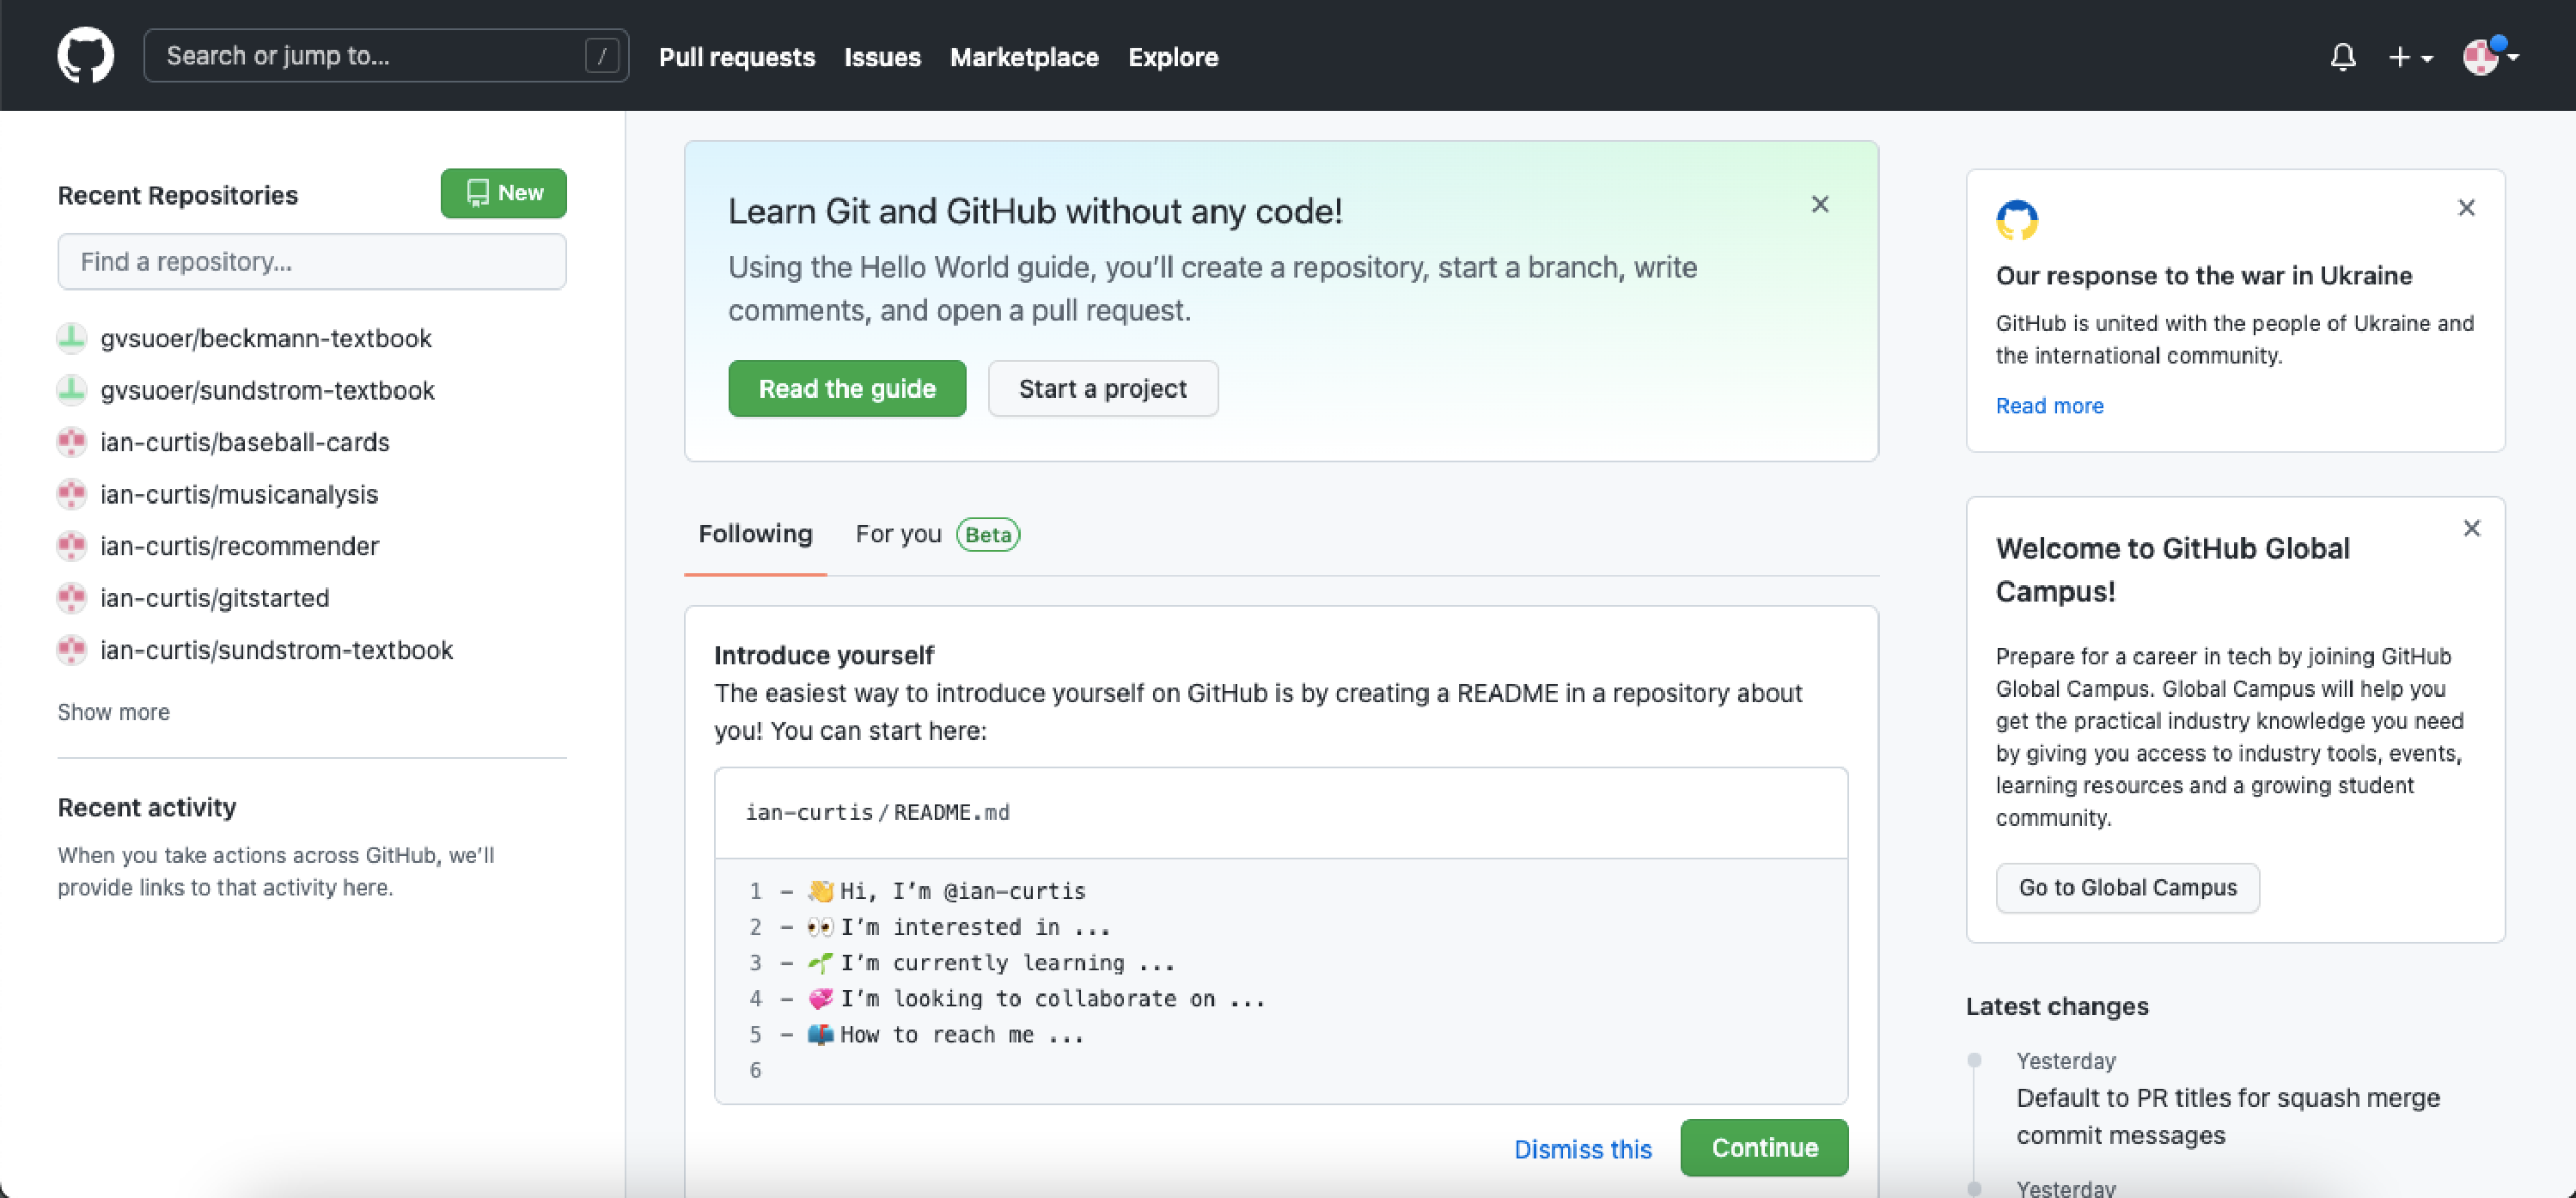
\includegraphics[width=\linewidth]{external/hub_home.pdf}
\end{image}%
\tcblower
\end{figureptx}%
Your profile page can be found by clicking on the robot-y icon (see \hyperref[figure-fig-hub-navbar]{Figure~{\xreffont\ref{figure-fig-hub-navbar}}}) in the top right and clicking on ``Your profile''. (Notice that the URL uses your username.) You probably don't see much. That's ok, you haven't created anything yet! On this page (the ``Overview'' tab) you can see your popular repositories, a graph of your contributions and a summary of your activity. Check out \href{https://github.com/ian-curtis}{my profile page}\footnote{\nolinkurl{github.com/ian-curtis}\label{fn-hub-profile-i-e}} for an example.%
\begin{figureptx}{Figure}{The GitHub Navigation Bar}{figure-fig-hub-navbar}{}%
\begin{image}{0.35}{0.3}{0.35}{}%
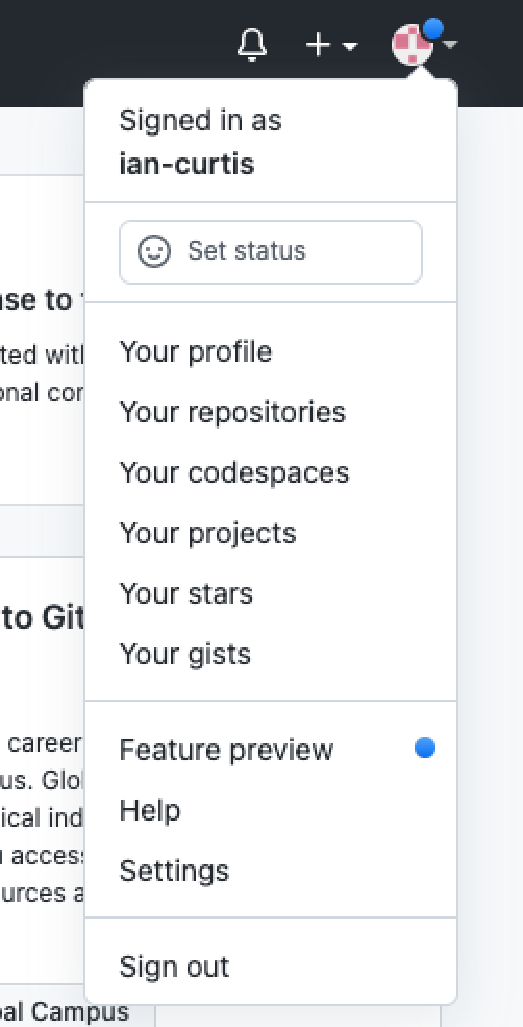
\includegraphics[width=\linewidth]{external/hub_navbar.pdf}
\end{image}%
\tcblower
\end{figureptx}%
First, you can edit your basic profile information on the left hand side including your profile image, name, bio, and location. I would recommend filling as much of that out as possible; it allows companies and other people to find you and confirm that you are who you are.%
\par
Wait a minute, I just used an unfamiliar word: repository. Essentially, a \terminology{repository} is the Git\slash{}GitHub way to say ``directory'' or ``folder''. A repository is usually one project; one repository contains all of the files and information for one project. For example, the files for this book can all be found under my repository titled \href{https://github.com/ian-curtis/gitstarted}{gitstarted}\footnote{\nolinkurl{github.com/ian-curtis/gitstarted}\label{fn-hub-profile-l-e}}. This book constitutes as one project and therefore all files for this book are there. Remember Jennifer Bryan from above? All of the files for her book, \pubtitle{Happy Git With R} can be found on \href{https://github.com/jennybc/happy-git-with-r}{her repository}\footnote{\nolinkurl{github.com/jennybc/happy-git-with-r}\label{fn-hub-profile-l-h}}. Soon, you too will have repositories! (Note: a repository is often shortened to just \terminology{repo}.)%
\par
There are a few other tabs at the top of the page. The ``Repositories'' tab simply lists all of your repos. (You can also find this page from the drop-down menu by your profile image in the top right.) The other three are not important for basic use (I haven't even used them yet).%
\end{subsectionptx}
%
%
\typeout{************************************************}
\typeout{Subsection 3.1.3 Settings and Customizations}
\typeout{************************************************}
%
\begin{subsectionptx}{Subsection}{Settings and Customizations}{}{Settings and Customizations}{}{}{subsection-hub-settings}
\index{github!settings}%
\index{github!customize}%
Click on the profile icon in the top right (\hyperref[figure-fig-hub-navbar]{Figure~{\xreffont\ref{figure-fig-hub-navbar}}}) and select ``Settings''. Don't be scared of the long list of possible customizations that are available. Most are only applicable to experienced GitHub users. I will introduce the settings you may be interested in right now. The headings of the following paragraphs match up with the headings of the tabs on the GitHub page. Note that some tabs have been excluded as well as some settings within some tabs. This does not mean that they are not important; it just means that I don't think they are necessary for a beginner.%
\begin{paragraphs}{Profile.}{paragraphs-hub-settings-e}%
\index{github!profile}%
Here, you can change your name, public email (if you have multiple AND if you have chosen to make your email public), a mini bio, relevant info about your other social media and company, location, and whether or not you are searching for a job. See \hyperlink{paragraphs-hub-emails}{Emails} for more info.%
\end{paragraphs}%
\begin{paragraphs}{Account.}{paragraphs-hub-settings-f}%
\index{github!account}%
Here is where you can change your username. \emph{I would strongly recommend against changing your username except in dire circumstances.} This could lead to broken links or, if someone claims your old username, links to the wrong repository. This is why I hope you took the time to really think of a good username when created your account.%
\par
Ok fine. If you have just created your account, have no repositories, have done pretty much nothing on GitHub other than editng settings, AND are truly unhappy with your username, change it now. NOW. Then try not to do it again.%
\par
This tab will also let you delete your entire account. It is in red for a reason. I would highly recommend never deleting your account. Even if you are done with GitHub and don't plan on ever using it again, others can still benefit from your code. Obviously some exceptions could apply here but for most purposes, you probably shouldn't delete your account.%
\end{paragraphs}%
\begin{paragraphs}{Appearance.}{paragraphs-hub-settings-g}%
\index{github!appearance}%
Here you can change how GitHub looks. Is white annoying? Switch to a dark theme. There are three of them. You can choose to have it change automatically with your computer (assuming your computer changes automatically). You can also edit the default emoji appearance.%
\par
There is currently a feature in testing allowing a theme designed for colorblind users. To enable this, click on your avatar in the top right and select ``Feature preview'', then ``Colorblind Themes'', then ``Enable''. If you have feedback to give GitHub, you can also do that.%
\end{paragraphs}%
\begin{paragraphs}{Account security.}{paragraphs-hub-settings-h}%
\index{github!security}%
Change your password here and you can enable two-factor authentication. You can also see where you are currently logged in. If an unfamiliar session is active, I would recommend changing your password and\slash{}or enabling two-factor authentication.%
\end{paragraphs}%
\begin{paragraphs}{Billing \& plans.}{paragraphs-hub-settings-i}%
\index{github!billing}%
GitHub offers different \href{https://github.com/pricing}{paid plans}\footnote{\nolinkurl{github.com/pricing}\label{fn-hub-settings-i-c-b}}. Each of the plans has its own benefits (e.g., more storage, more collaborators) but the GitHub essentials work perfectly fine under the free plan and many people do not upgrade. Once you become more familiar with Git, GitHub, and start developing more projects, you might like an upgrade. However, there is no need to pay anything at this point.%
\par
Bonus! Students get free GitHub Pro and access to a multitude of extra deals with their \href{https://education.github.com/pack}{Student Developer Pack}\footnote{\nolinkurl{education.github.com/pack}\label{fn-hub-settings-i-d-b}}. \href{https://education.github.com/teachers}{Teachers}\footnote{\nolinkurl{education.github.com/teachers}\label{fn-hub-settings-i-d-d}} and \href{https://education.github.com/schools}{Schools}\footnote{\nolinkurl{education.github.com/schools}\label{fn-hub-settings-i-d-f}} can also find benefits (some require a payment).%
\end{paragraphs}%
\begin{paragraphs}{Emails.}{paragraphs-hub-emails}%
\index{github!emails}%
You can choose to have multiple emails on your GitHub account. This may be something you want to do as you can also select to have one of your emails be a backup email for security. You can also select if you would like to keep your emails private or not. I currently have two emails on my account: my main, non-school email and my school's \mono{.edu} email (so I can use my student discounts on my account without creating a new account).%
\end{paragraphs}%
\begin{paragraphs}{Notifications.}{paragraphs-hub-settings-k}%
\index{github!notifications}%
Pretty simple here. You can choose which notifications you would like to receive. Maybe keep the defaults for now and you can edit them later when you get an idea of what exactly GitHub sends notifications for. I still have the defaults selected and I don't get many emails at all.%
\end{paragraphs}%
\begin{paragraphs}{Repositories.}{paragraphs-hub-settings-l}%
\index{github!repository}%
\index{repository}%
If you just created your account, this is probably empty. That's ok! It will be populated soon with a list of all your repositories and repositories you have access to. I do want to point out the first setting, ``Repository default branch''. It may say ``master'' in the text box. If so, please change it to ``main'' (by typing and clicking ``Update'' which is the new Git\slash{}GitHub standard.%
\par
For more information on the transition from ``master'' to ``main'', please visit \href{https://www.theserverside.com/feature/Why-GitHub-renamed-its-master-branch-to-main}{TheServerSide}\footnote{\nolinkurl{theserverside.com/feature/Why-GitHub-renamed-its-master-branch-to-main}\label{fn-hub-settings-l-e-d}}.%
\end{paragraphs}%
\begin{paragraphs}{Blocked Users.}{paragraphs-hub-settings-m}%
\index{github!blocked}%
Hopefully you won't ever have to, but if you need to block a user, you can do so here.%
\end{paragraphs}%
\end{subsectionptx}
\begin{conclusion}{}%
Hopefully you now have an idea of how GitHub is organized and are aware of the customizations you can make. However, we have barely scratched the surface of what GitHub can do. In the next section, you will create your own repository and learn some GitHub vocabulary.%
\end{conclusion}%
\end{sectionptx}
%
%
\typeout{************************************************}
\typeout{Section 3.2 The First Repository and File}
\typeout{************************************************}
%
\begin{sectionptx}{Section}{The First Repository and File}{}{The First Repository and File}{}{}{section-S_hubfirstrepo}
\index{github!repository}%
\index{repository}%
\begin{introduction}{}%
Buckle your seatbelts! Here we go into GitHub and the first repository. In this section, we will create a repository with some information about ourselves. I recommend that you don't just read the book; follow along with your own account. Practice makes improvement!%
\end{introduction}%
%
%
\typeout{************************************************}
\typeout{Subsection 3.2.1 Creating a Repository}
\typeout{************************************************}
%
\begin{subsectionptx}{Subsection}{Creating a Repository}{}{Creating a Repository}{}{}{subsection-hub-createrepo}
\index{github!create repository}%
There are a few different ways to create a new repo (remember this abbreviation? see \hyperref[subsection-hub-profile]{Subsection~{\xreffont\ref{subsection-hub-profile}}}).%
\begin{enumerate}
\item{}In the top right of the page, next to the profile avatar we saw in \hyperref[section-S_hubnavigate]{Section~{\xreffont\ref{section-S_hubnavigate}}}, there is a plus (+) sign. Click on that and then ``new repository''.%
\par
Note: GitHub differentiates bewteen a repository and a project. Don't get confused. We want repository (and you will want that for most purposes).%
\item{}From the \href{https://github.com}{GitHub homepage}\footnote{\nolinkurl{github.com}\label{fn-hub-createrepo-c-b-b-a-b}} there is a section on the left called ``Repositories''. Next to the title is a button that says ``New''. Click on that.%
\item{}If you navigate to the profile avatar in the top right, and click on ``Your repositories'', there will also be a ``New'' button near the top.%
\end{enumerate}
Each of these three methods will get you to the same page. It doesn't matter which one you click.%
\begin{figureptx}{Figure}{Various methods to create a new repo}{figure-fig-hub-new-repo}{}%
\begin{sidebyside}{2}{0.025}{0.025}{0.05}%
\begin{sbspanel}{0.45}%
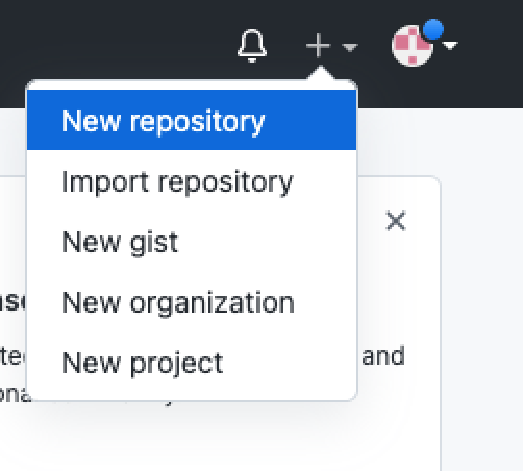
\includegraphics[width=\linewidth]{external/hub_new_repo_navbar.pdf}
\end{sbspanel}%
\begin{sbspanel}{0.45}%
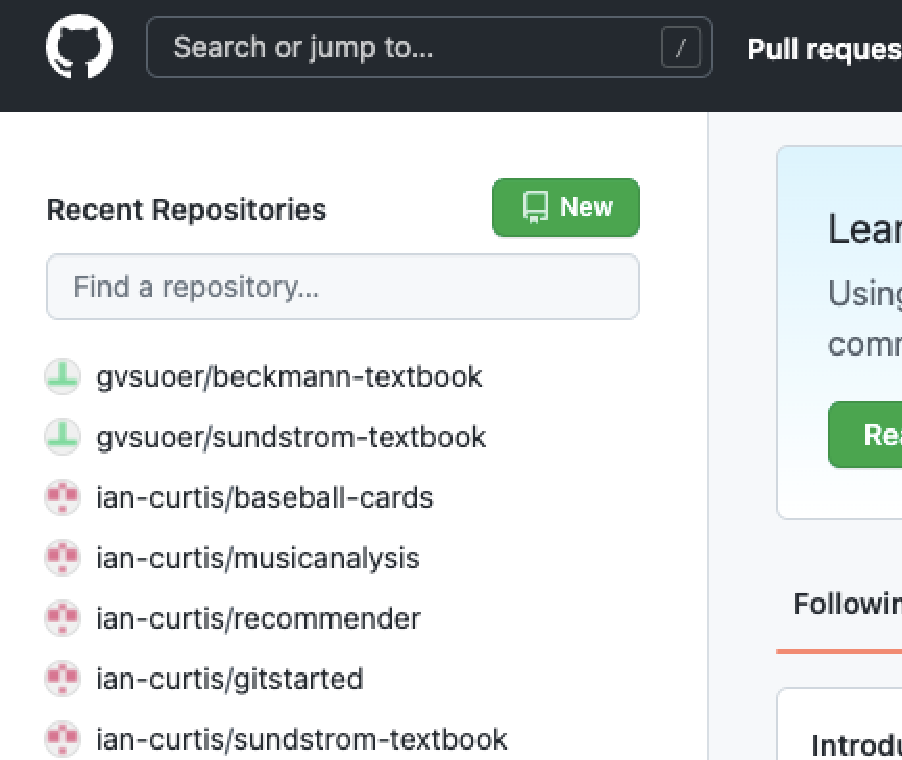
\includegraphics[width=\linewidth]{external/hub_new_repo_home.pdf}
\end{sbspanel}%
\end{sidebyside}%
\tcblower
\end{figureptx}%
\begin{figureptx}{Figure}{Another method to create a new repo}{figure-hub-createrepo-e}{}%
\begin{image}{0.05}{0.9}{0.05}{}%
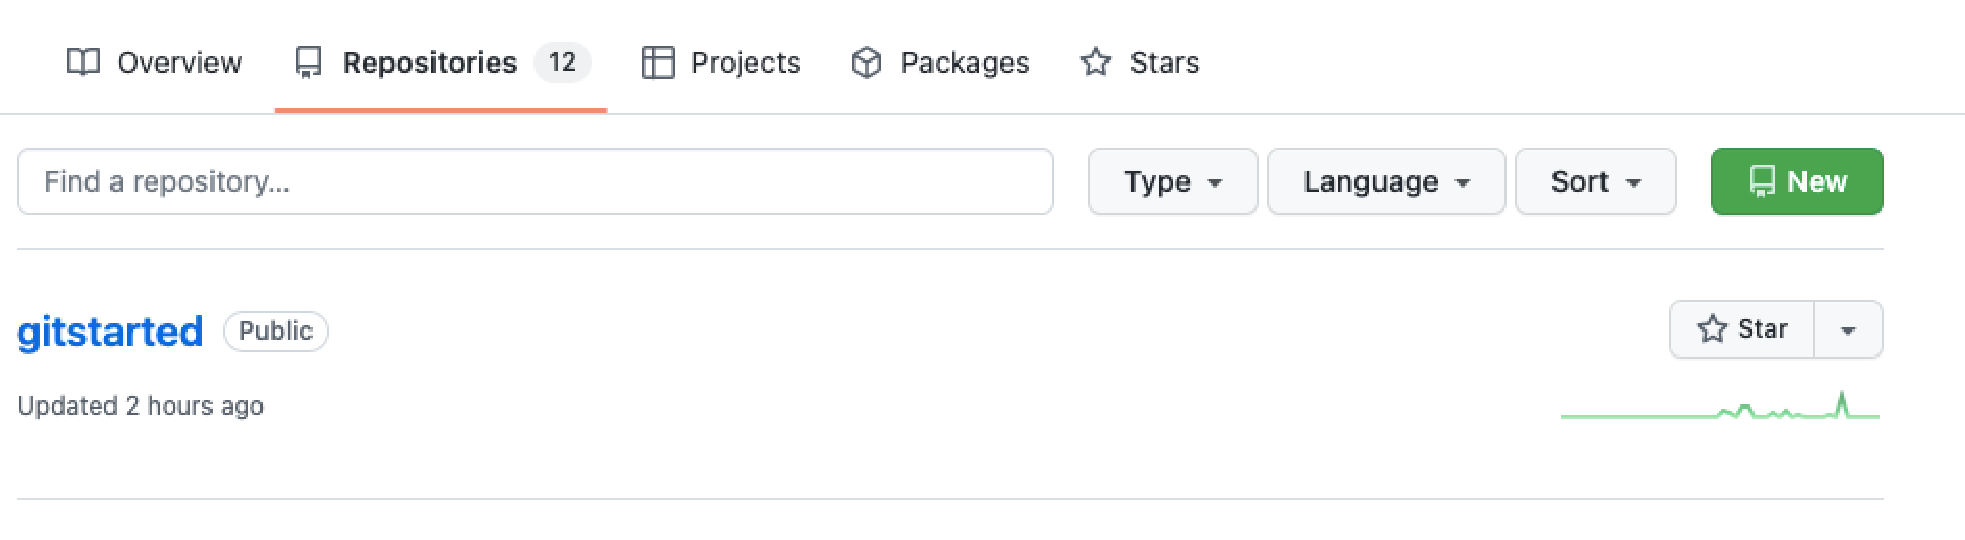
\includegraphics[width=\linewidth]{external/hub_new_repo_yourrepos.pdf}
\end{image}%
\tcblower
\end{figureptx}%
\begin{inlineexercise}{Checkpoint}{}{exercise-hub-createrepo-f}%
Let's begin the process of creating our first repo. Use one of the methods above get into the ``Create a new repository'' screen (\hyperref[figure-fig-hub-new-repo-screen]{Figure~{\xreffont\ref{figure-fig-hub-new-repo-screen}}}).%
\end{inlineexercise}%
\begin{figureptx}{Figure}{The New Repository Screen}{figure-fig-hub-new-repo-screen}{}%
\begin{image}{0.05}{0.9}{0.05}{}%
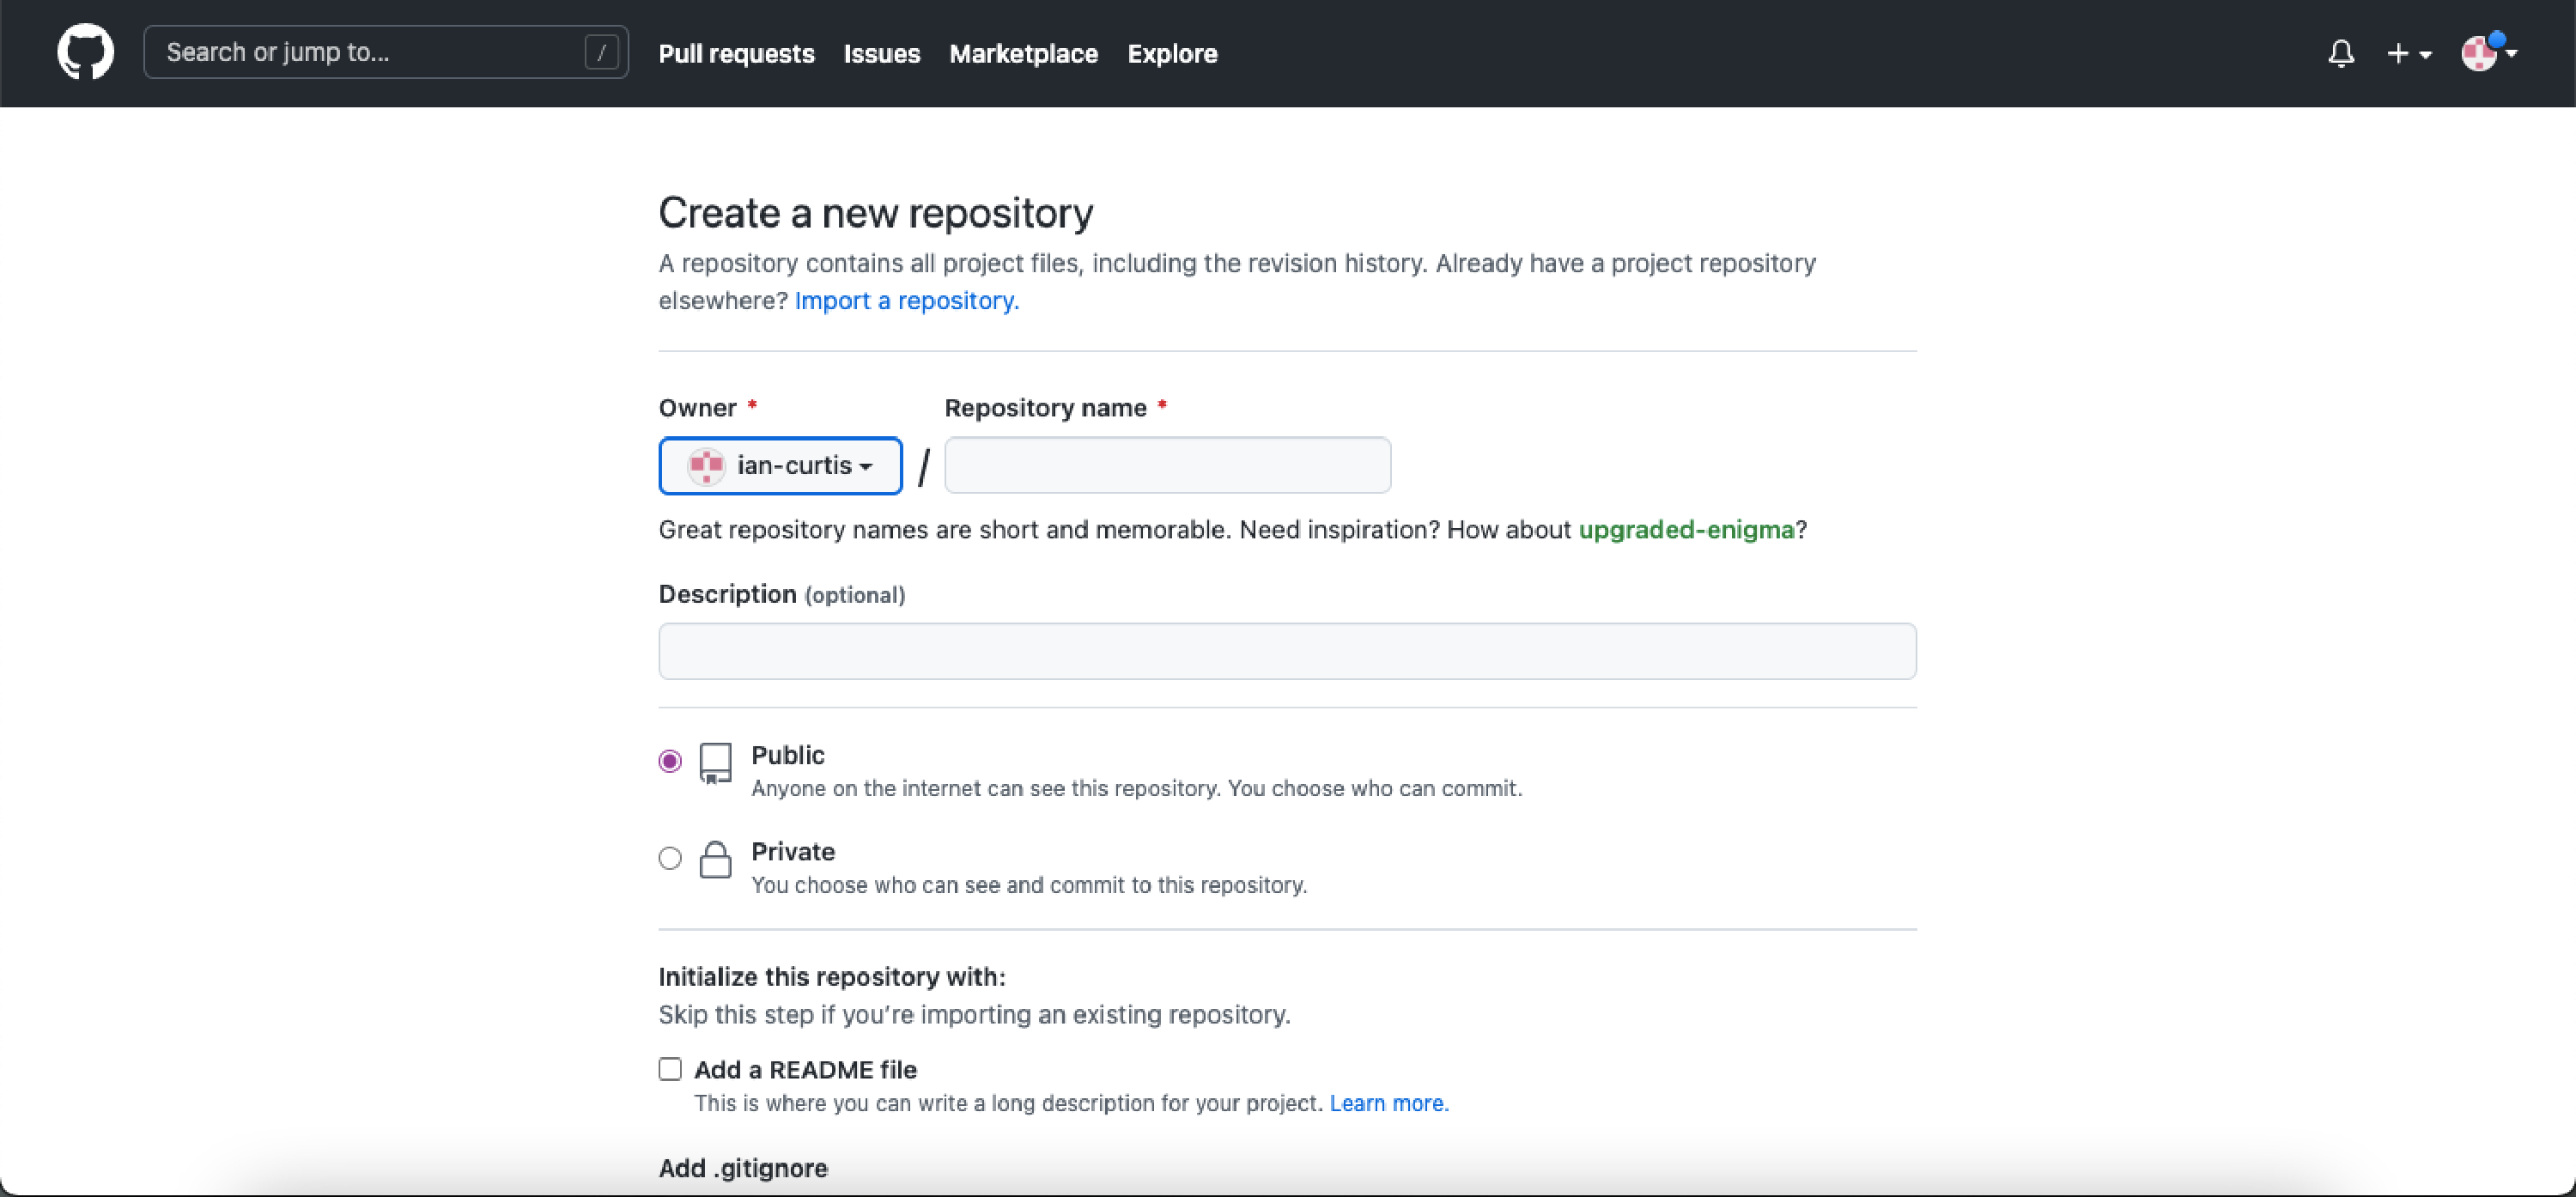
\includegraphics[width=\linewidth]{external/hub_new_repo_screen.pdf}
\end{image}%
\tcblower
\end{figureptx}%
It is not difficult to create a repo. It is difficult, however, to come up with a repo name. Repository name requirements are similar to the conventions for file and folder names (\hyperref[section-S_filenames]{Section~{\xreffont\ref{section-S_filenames}}}) in that they can have no spaces and should briefly describe what the repo is for. \emph{Please take the time to think about your repo names before you create them.} Renaming repositories is possible, but can cause complications in the future (such as broken links). Again, names should be short, to the point, and descriptive. The repo name for this book is ``gitstarted'', the shortened title.%
\par
If you are thinking ``Wait! I don't know the details of my project!'' then you are not alone. The problem with this is that you have to decide what your repo is going to be about before you name it. I have definitely been victim to this and have made some rather stupid names that I should've made better. For right now, I will tell you what to name your repo. In the future, it might be best to start with a private repo and then change the name (if you need to) before you make it public. Otherwise, just be aware that there may be consequences should you change it at any other time.%
\par
In the ``Repository name'' box, type the name \mono{aboutme}. Adding a description is optional and is not necessary for us right now. Next is the viewability. You may choose to make your repos private (only you and authorized collaborators can view\slash{}edit) or public (everyone can view and attempt to edit, only you and authorized collabortors can approve edits). It does not matter what you select for this; do whatever your heart desires.%
\par
\index{readme}\index{license}\index{gitignore} The next step deals with certain files that can be automatically added to your repo. You have the choice for either or none of a \mono{README} file, a \mono{.gitignore}, and a license. A \terminology{README file} gives all the pertinent information about your repository in an easy-to-read format. It is often the first thing that people visiting your repo will read and is very important. Check this box and we will come back to the \mono{README} file in just a minute. A \terminology{gitignore} file tells Git all of the files \emph{not} to put online. Do not check this box for now; it will be very useful later on, but is not needed now. You can also choose to put a \terminology{license} on your code which lets users know what they can and cannot do. If you would like to explore the different licenses, please visit \href{https://docs.github.com/en/repositories/managing-your-repositorys-settings-and-features/customizing-your-repository/licensing-a-repository}{the GitHub documentation}\footnote{\nolinkurl{docs.github.com/en/repositories/managing-your-repositorys-settings-and-features/customizing-your-repository/licensing-a-repository}\label{fn-hub-createrepo-k-l}}. You are welcome to choose a license if you'd like, but it is not necessary at this time.%
\par
You now should have entered ``aboutme'' into the name box, selected if you wanted the repo to be public or private, and checked the \mono{README} box. Now, click the ``Create repository'' button to finalize the process.%
\end{subsectionptx}
%
%
\typeout{************************************************}
\typeout{Subsection 3.2.2 Exploring the Code Tab}
\typeout{************************************************}
%
\begin{subsectionptx}{Subsection}{Exploring the Code Tab}{}{Exploring the Code Tab}{}{}{subsection-hub-explorerepo}
\index{github!code tab}%
Whew, we made it! A new repo has just been created\textellipsis{}aaaaand a lot of new buttons and options just appeared. A lot of new unfamiliar words and tabs. Please don't give up here! I will go through all of the important aspects. Many of the pieces are not applicable to beginners and some will not be applicable until we start working with Git and GitHub together. In this section, I will only be explaining the key features and will slowly add in more as we learn more about GitHub.%
\begin{figureptx}{Figure}{The new repository tabs}{figure-fig-hub-repo-tabs}{}%
\begin{image}{0.1}{0.8}{0.1}{}%

\includegraphics[width=\linewidth]{external/hub_repo_tabs.pdf}
\end{image}%
\tcblower
\end{figureptx}%
Assuming you didn't click on anything, you should see a pretty empty page. In the top left, you should see your username and your repo name. This is common throughout GitHub so you always know where you are. Underneath that is a set of tabs that can be used to navigate through the repository-level settings and options (see \hyperref[figure-fig-hub-repo-tabs]{Figure~{\xreffont\ref{figure-fig-hub-repo-tabs}}}). You should currently be on the ``Code'' tab. As may be expected, this tab displays all of the files associated with the repo; it is the ``home page'' for every repository. You should see that a \mono{README.md} file shows up. Also notice that the contents of the README are displayed under the list of files. GitHub knows how important the READMEs are to explaining code that it automatically displays the contents of the file. Right now, ours is empty (except for the default title).%
\par
To summarize, this is all you should care about for now:%
\begin{itemize}[label=\textbullet]
\item{}The navigation at the top%
\item{}The content of the ``Code'' tab%
\item{}Noticing our README file in the list of files%
\item{}Noticing the contents of the README file underneath the list of files%
\end{itemize}
%
\end{subsectionptx}
%
%
\typeout{************************************************}
\typeout{Subsection 3.2.3 Editing a File}
\typeout{************************************************}
%
\begin{subsectionptx}{Subsection}{Editing a File}{}{Editing a File}{}{}{subsection-hub-editfile}
\index{github!edit files}%
Well, we have a README file, let's edit it! GitHub makes it rather simple to edit files. There are a two main ways to edit the README file on GitHub:%
\begin{enumerate}
\item{}Click on the file name \mono{README.md} in the list of files. Click on the pencil icon on the right of the header of the README file (\hyperref[figure-fig-hub-edit-readme]{Figure~{\xreffont\ref{figure-fig-hub-edit-readme}}}).%
\item{}Click on the pencil icon found along the header of the README file (under the list of files). See \hyperref[figure-fig-hub-edit-readme2]{Figure~{\xreffont\ref{figure-fig-hub-edit-readme2}}}.%
\end{enumerate}
%
\begin{figureptx}{Figure}{One way to edit a README file (on the Code tab)}{figure-fig-hub-edit-readme}{}%
\begin{image}{0.05}{0.9}{0.05}{}%

\includegraphics[width=\linewidth]{external/hub_edit_readme_code.pdf}
\end{image}%
\tcblower
\end{figureptx}%
\begin{figureptx}{Figure}{Another way to edit a README file (on the README file)}{figure-fig-hub-edit-readme2}{}%
\begin{image}{0.05}{0.9}{0.05}{}%
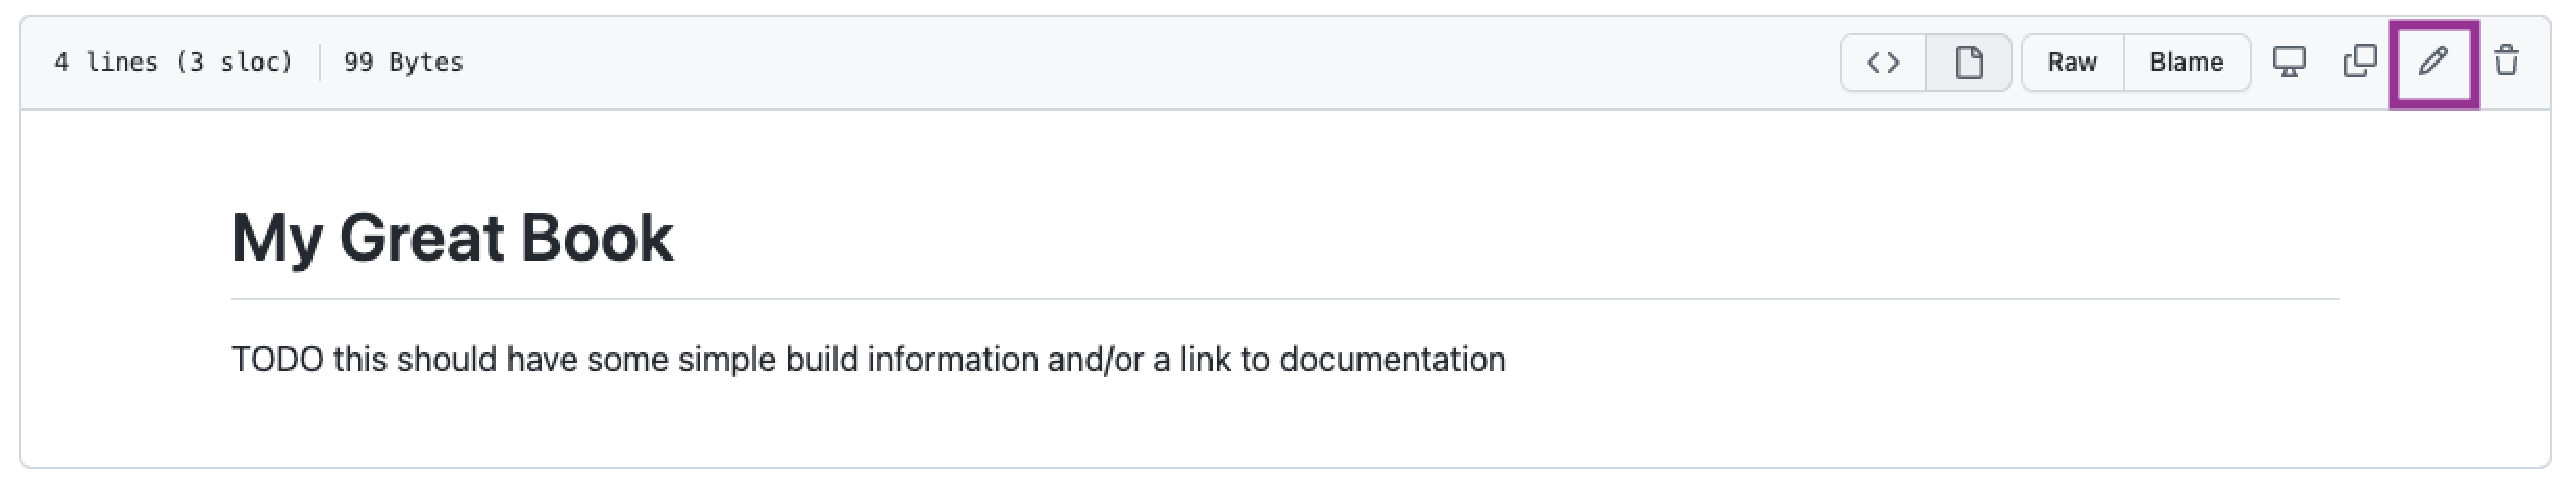
\includegraphics[width=\linewidth]{external/hub_edit_readme_file.pdf}
\end{image}%
\tcblower
\end{figureptx}%
\begin{inlineexercise}{Checkpoint}{}{exercise-hub-editfile-f}%
Use one of the methods above to open the README file and get to its editing screen.%
\end{inlineexercise}%
As discussed in \hyperref[section-S_fileextensions]{Section~{\xreffont\ref{section-S_fileextensions}}}, a file ending with \mono{.md} is a markdown file. All README files should be markdown files and are able to understand markdown syntax. Essentially, markdown allows us to communicate basic word processing functions simply by typing certain symbols. Have you ever noticed that you can't bold or italicize text in Google? \kbd{Control} (\kbd{Command}) + \kbd{B} or \kbd{I} don't work there! They also won't work in markdown files, unfortunately. But that doesn't mean we can't bold or italicize text. I will not discuss everything on markdown here, so some basic functions are below. It will be in your best interest to become familiar with markdown and its more advanced features sooner rather than later.%
\begin{assemblage}{Assemblage}{Markdown Basics.}{assemblage-markdown}%
The most basic markdown tool is simple text. Just type like you normally would into the text field and the result will be normal, unformatted text. However\textellipsis{}%
\begin{itemize}[label=\textbullet]
\item{}To italicize a word or phrase, put one asterisk around it: \mono{I\textquotesingle{}m *very* happy I won the lottery!}%
\item{}To bold a word or phrase, put two asterisks around it: \mono{If a zombie comes, make sure you **run**.}%
\item{}To create headings, place hashtags (pound signs, if you insist) and a space before the text you wish to be in the heading: \mono{\# A Title}. The more hashtags you add, the deeper the heading level. Thus, \mono{\#\# A Subheading} is a level two heading whereas \mono{\#\#\# Another Subheading} is a level three heading.%
\item{}To create a bulleted list, start a line with an asterisk (\textasteriskcentered{}) and a space. For numbered lists, start a line with a number and a period (and a space). Make sure you start each list item on a new line, like so:%
\begin{codedisplay}
* Green Eggs and Ham
* Wocket (it might be in your pocket)
* Fiffer Feffer Feff
* Truffula Trees
* Sneetches and Thneeds
\end{codedisplay}
%
\item{}To put words into a code cell, place a backtick around the code: \mono{\textasciigrave{}import requests\textasciigrave{}}. (The backtick is located to the left of the 1 key on American keyboards.)%
\end{itemize}
You can also add images, gifs, links, links with text intead of urls, tables, and multi-line code chunks. For more information, see \href{https://www.markdownguide.org/basic-syntax/}{Basic Markdown Syntax}\footnotemark{} and \href{https://www.markdownguide.org/extended-syntax/}{Extended Markdown Syntax}\footnotemark{}.%
\par
It is also important to note that GitHub Markdown differs slightly from other flavors of Markdown. See \href{https://gist.github.com/vimtaai/99f8c89e7d3d02a362117284684baa0f}{a nice table from GitHub user vimtaai}\footnotemark{}.%
\end{assemblage}
\footnotetext[44]{\nolinkurl{www.markdownguide.org/basic-syntax/}\label{fn-markdown-c-d}}%
\footnotetext[45]{\nolinkurl{www.markdownguide.org/extended-syntax/}\label{fn-markdown-c-f}}%
\footnotetext[46]{\nolinkurl{gist.github.com/vimtaai/99f8c89e7d3d02a362117284684baa0f}\label{fn-markdown-d-b}}%
\begin{inlineexercise}{Checkpoint}{}{exercise-try-markdown}%
\index{markdown}%
Let's practice your markdown skills! Here, you will make the "aboutme" repo name true. Feel free to use the guidelines and sources above. You could also search online if you aren't sure how to do what you want to do. I have provided my (basic) example \href{https://github.com/ian-curtis/gitstarted}{in the repo for this book}\footnotemark{} (titled \mono{README\_aboutme.md} in the \mono{book-activities} folder). There will be extra sections in my document that aren't required of you here (these will come later in future activities). Be creative! There aren't any ``right'' answers.%
\par
Github is pretty cool in that it will show you realtime updates of what your Markdown file will look like after you're done typing. There is a ``Preview'' tab right above the first line of your README file (you are currently on ``Edit file''). After each task below, check the preview to verify that what you typed worked as expected.%
\begin{enumerate}[font=\bfseries,label=(\alph*),ref=\alph*]%
\item{}Currently, the title of the README is the repo name. Change the title to a more human-readable one.%
\item{}In the first paragraph, type your name (or your username), how many pets you have, and your favorite hobby.%
\item{}In a second paragraph, type a sentence stating who your favorite music artist is. Then, make an ordered list of your favorite songs from that artist.%
\item{}Create a heading level two titled ``Oh Look, More Things About Me''%
\item{}In a third paragraph, write two sentences with two cool facts about you. These could be made up, no one will know! After that paragraph, create an unordered list of your favorite musical artists.%
\item{}Go back to the previous paragraphs and bold two words and italicize two words.%
\item{}Extra Credit: Add an image, a nested list of your favorite colors and why they are your favorite, a link to your favorite YouTube video, and, if you know a coding language, some code.%
\par
No worries if you can't get any of these to work! This task is simply here to help you explore Markdown a little bit.%
\par\smallskip%
\noindent\textbf{\blocktitlefont Hint}.\hypertarget{hint-try-markdown-i-b}{}\quad{}To add images, you will need to make sure you specify the correct filepath to the image. This can be hard to get right as it depends on where the image is saved and where your Markdown file lives on your computer. If the image doesn't appear at first, you might try making sure the image and the Markdown file are in the same folder and seeing if things work out better.%
\end{enumerate}%
Don't leave your file yet! There's one more thing left to do.%
\end{inlineexercise}%
\footnotetext[47]{\nolinkurl{github.com/ian-curtis/gitstarted}\label{fn-try-markdown-b-a-b}}%
\begin{figureptx}{Figure}{The GitHub Commit Changes Dialog}{figure-fig-hub-commit}{}%
\begin{image}{0.15}{0.7}{0.15}{}%
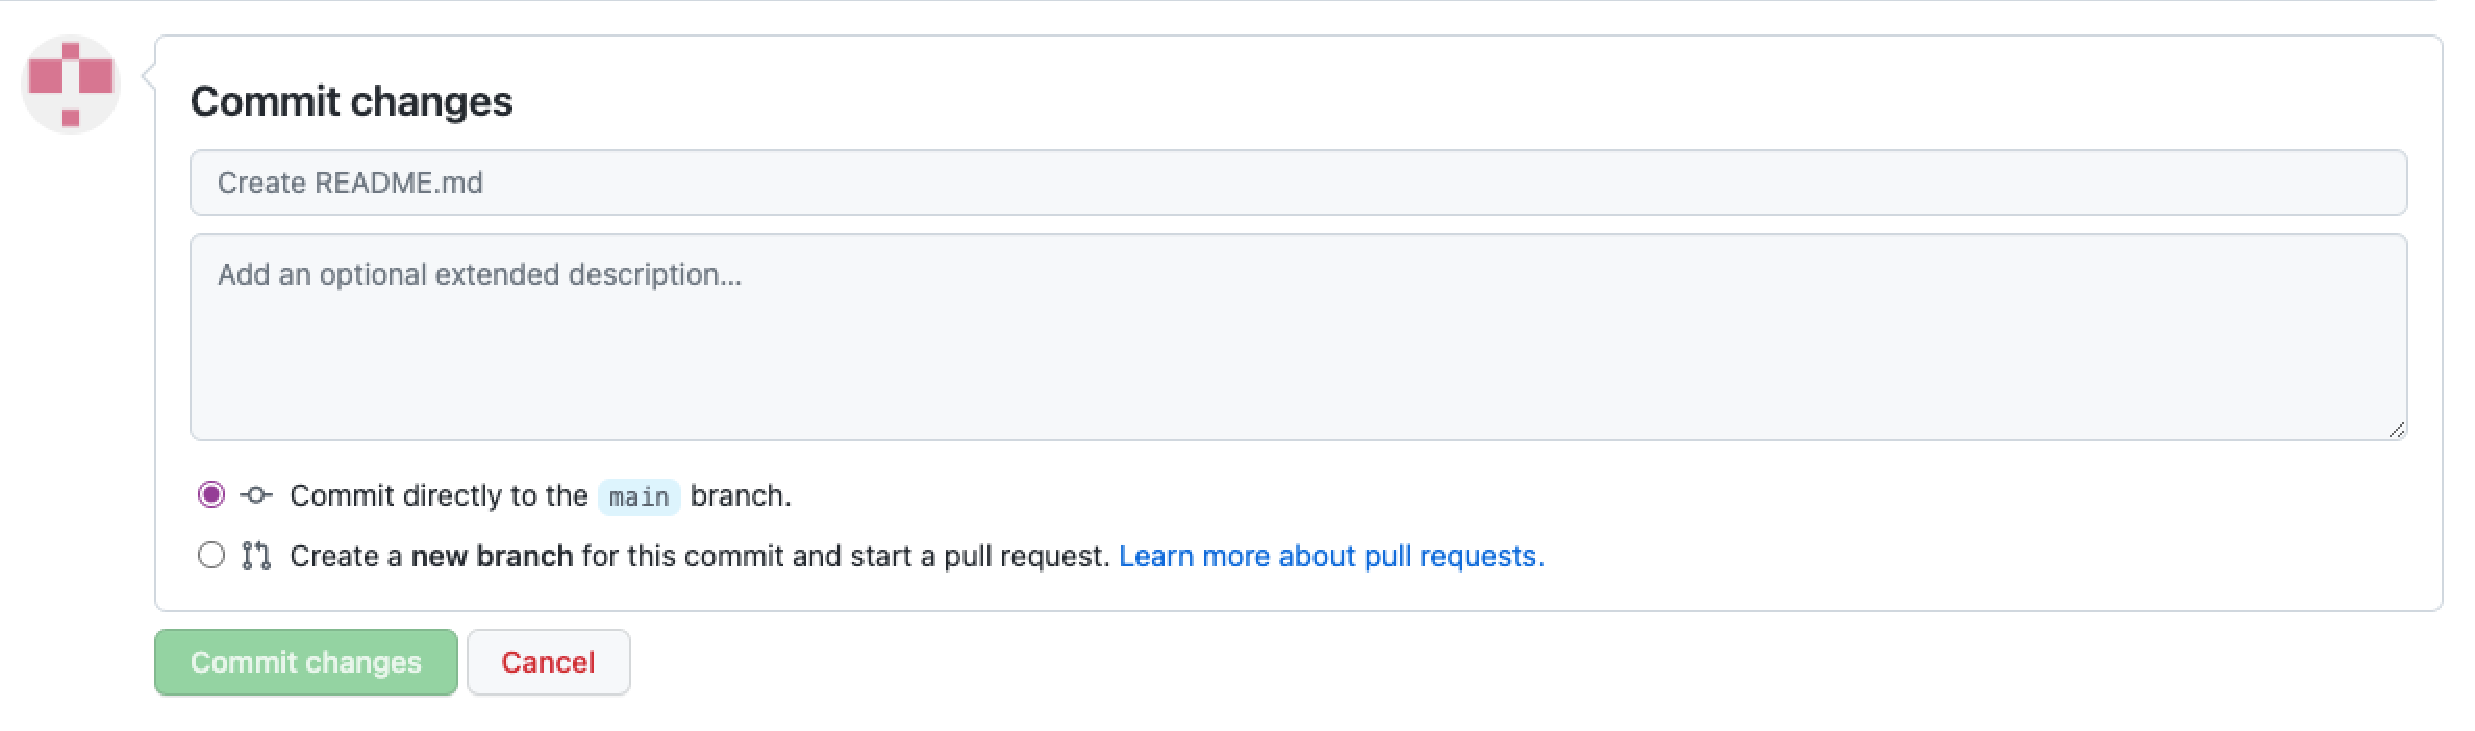
\includegraphics[width=\linewidth]{external/hub_commit.pdf}
\end{image}%
\tcblower
\end{figureptx}%
\index{commit}\index{commit changes|see{commit}}\index{github!commit} Right now, we have only edited the file, but we haven't told Github that we wish to keep our edits. It's as if we edited a document, but never clicked save! But if you head to the top right of the editing window, you'll see that there is no ``save'' button. You should see a ``Commit changes...'' button, as in \hyperref[figure-fig-hub-commit]{Figure~{\xreffont\ref{figure-fig-hub-commit}}}. This is important. Github uses \terminology{commit} when indicating that you are about to officially upload your changes to your repo. This is your last change to change anything.%
\par
When you think you are done editing the file, go ahead and use the ``Commit changes'' buttom to commit your changes (leave the ``commit directly to the main branch'' option selected). Your changes should be represented. Navigate back to the Code tab and scroll down to your README to make sure of this.%
\par
Take care to notice the difference between committing and saving. Saving is easy. You can add a word, then save. Add a word, save. And so on. Think of commiting as adding a word, saving, \emph{and closing the document}. Now every time you want to add another word you have to open the entire document again, add the word, save, and close the document again. This system is put in place to help with version control. Instead of there being one version for each new word you add, there is one version for each commit. Each commit represents a stamp on the version control timeline. When coding, you should certainly save your files as you go, but you commit your changes less often than you save. This will become more apparent when we work with Git and with multiple files.%
\par
It might be worth saying again just to make sure you've got it. Instead of there being one version for each new word you add, there is one version for each commit. Projects are typically broken up into tiny pieces. Each of these pieces would correspond to a commit. So if something goes wrong, you can revert back to a previous commit. We don't want commits to be for every word since it would take forever to find the commit you want to revert to. Conversely, we don't want commits to contain too many edits as that would require more work to rebuild your files if you had to revert backwards.%
\begin{assemblage}{Assemblage}{An Extra Commit Example.}{assemblage-ex-commit}%
Let's consider one example to help understand the benefits of thinking in commits. Suppose I was working on a small video game and I was tasked with creating different worlds a character could visit. With commits in mind, I decide to break down the task into chunks: I will build one world at a time. When I am done with one world, I will commit. When I am done with another world, I will commit a second time. And so on.%
\par
This is different than creating a window in a building in the first world, then saving. Then creating two more windows and a door, then saving. Then adding some a tree and some flowers, then saving. We save much more often than we commit. But \emph{we save using our computer and commit using Git\slash{}Gitub.} I would never save to Github or commit to my computer. Saving is light, commiting is heavy.%
\par
That being said, do make sure to save your files! You want to save your progress on your computer, but there is no need to commit after each time you save.%
\end{assemblage}
\end{subsectionptx}
\begin{conclusion}{}%
Hopefully, you now feel (at least slightly) more comfortable with the Code tab and editing a file on Github. The next chapter will look at branches which help with safely adding new features to our code.%
\end{conclusion}%
\end{sectionptx}
%
%
\typeout{************************************************}
\typeout{Section 3.3 Working With Branches}
\typeout{************************************************}
%
\begin{sectionptx}{Section}{Working With Branches}{}{Working With Branches}{}{}{section-S_hubbranches}
\index{branches}%
\index{github!branches}%
\begin{introduction}{}%
Suppose you were writing a three-stanza poem for a contest. The final product must be handwritten on fancy letterhead, in high-quality black pen. As multiple drafts go by, you finalize the first and the third stanza. You're so confident in them that you write them on the letterhead in pen. But you're stuck on the second stanza.%
\par
After some introspection and brainstorming, you finally come up with two potential second stanzas. But you can't decide between the two! You decide that the best way to figure out which one you like is to write each one in the poem and see if it flows with the rest. You can't just write one in the official poem (in pen!). What if the one you choose isn't what you like? Then you have to rewrite the entire poem.%
\par
Instead, you decide to get out two pieces of scratch paper and write the poem in pencil and with a respective second stanza. That way you can hold them side-by-side and compare their flow. This method makes it easier for you to decide which of the two candidates you prefer. Once you have done so, you write the final stanza in pen on the letterhead and recycle the scratch paper with your drafts.%
\par
Believe it or not, this potentially unrealistic example is a great demonstration of what Git and Github call \terminology{branches}. Branches will be used extensively in the coming sections and chapters and are quite important to smoothing out your workflow.%
\end{introduction}%
%
%
\typeout{************************************************}
\typeout{Subsection 3.3.1 Thinking About Branches}
\typeout{************************************************}
%
\begin{subsectionptx}{Subsection}{Thinking About Branches}{}{Thinking About Branches}{}{}{subsection-SS_thinkbranch}
\index{main branch}%
\index{branches}%
Github organizes your edits and changes in a tree-like format. The official, published version of your files always lies on the \terminology{main branch}. You could think of the main branch as the trunk of a tree. When we created our README file back in \hyperref[section-S_hubfirstrepo]{Section~{\xreffont\ref{section-S_hubfirstrepo}}}, we started on the main branch, edited a file, and commited right back to the main branch. It was as if we wrote something new in pen on our official letterhead. See \hyperref[figure-fig-commit-main-poem]{Figure~{\xreffont\ref{figure-fig-commit-main-poem}}} as a visualization of this type of commit.%
\begin{figureptx}{Figure}{Diagram of a commit from \mono{main} to \mono{main}}{figure-fig-commit-main-poem}{}%
\begin{image}{0.05}{0.9}{0.05}{}%
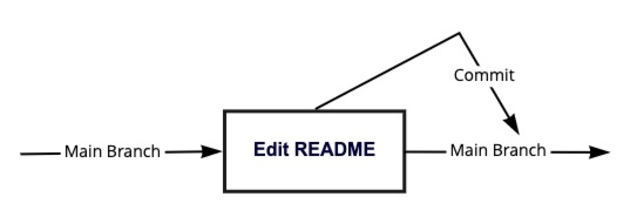
\includegraphics[width=\linewidth]{external/commit_main_poem.pdf}
\end{image}%
\tcblower
\end{figureptx}%
\emph{This type of editing is usually discouraged.} It is best practice to create a new branch, made some edits there, then submit a pull request to merge your changes into the main branch.%
\par
Whoa. I said a lot of stuff there. Lots of new words and things you don't know how to do. Don't worry, I'll guide you through it in this section. When you get a new project, you want to try and break it up into pieces. Each piece will have its own branch on the Github tree. For instance, the two poems that you wrote on scratch paper above were two branches off of the official poem. They each had the same first and third stanzas; only their second stanzas differed. See \hyperref[figure-fig-branch-poem]{Figure~{\xreffont\ref{figure-fig-branch-poem}}} for a visualization of branches in this instance.%
\begin{figureptx}{Figure}{Diagram of two branches off of main}{figure-fig-branch-poem}{}%
\begin{image}{0}{1}{0}{}%
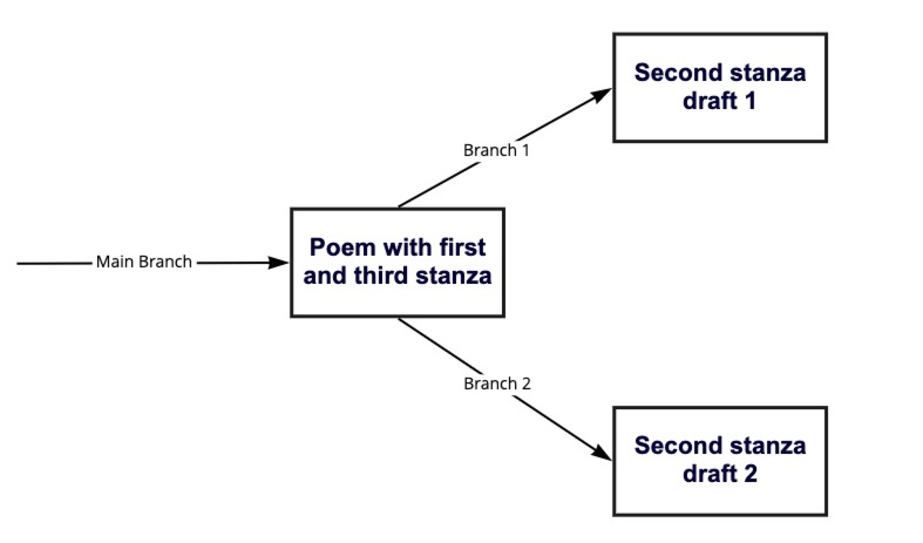
\includegraphics[width=\linewidth]{external/branch_poem.pdf}
\end{image}%
\tcblower
\end{figureptx}%
\index{commit}\index{merge}\index{pull request}\index{request|see{pull request}}\index{github!commit}\index{github!merge}\index{github!pull request} Notice how in \hyperref[figure-fig-branch-poem]{Figure~{\xreffont\ref{figure-fig-branch-poem}}} that the main branch does not move forward when branches are created, it stops once a branch is made. When you first create a new branch, all you have is a copy of the main branch. However, when you edit your new branch, the changes do not appear into the main branch. Branches are like testing grounds. Try some new things, see if you like them, see if they work, then make it official. ``Making it official'' with Git and Github is called \terminology{committing} (as we have seen). Two new terms that go with commits\footnote{Notice how ``commit'' is both a noun and a verb.\label{fn-SS_thinkbranch-i-k}} are \terminology{merge} and \terminology{pull request}. Oftentimes, you will hear people say that they just merged their changes into main. This means they committed their changes to the main branch and updated the official version. With the poem example, there are two possible merges you could make into main, as diagrammed in \hyperref[figure-fig-merge-poem]{Figure~{\xreffont\ref{figure-fig-merge-poem}}}.%
\begin{figureptx}{Figure}{Diagram showing a possible merge into main}{figure-fig-merge-poem}{}%
\begin{image}{0.05}{0.9}{0.05}{}%
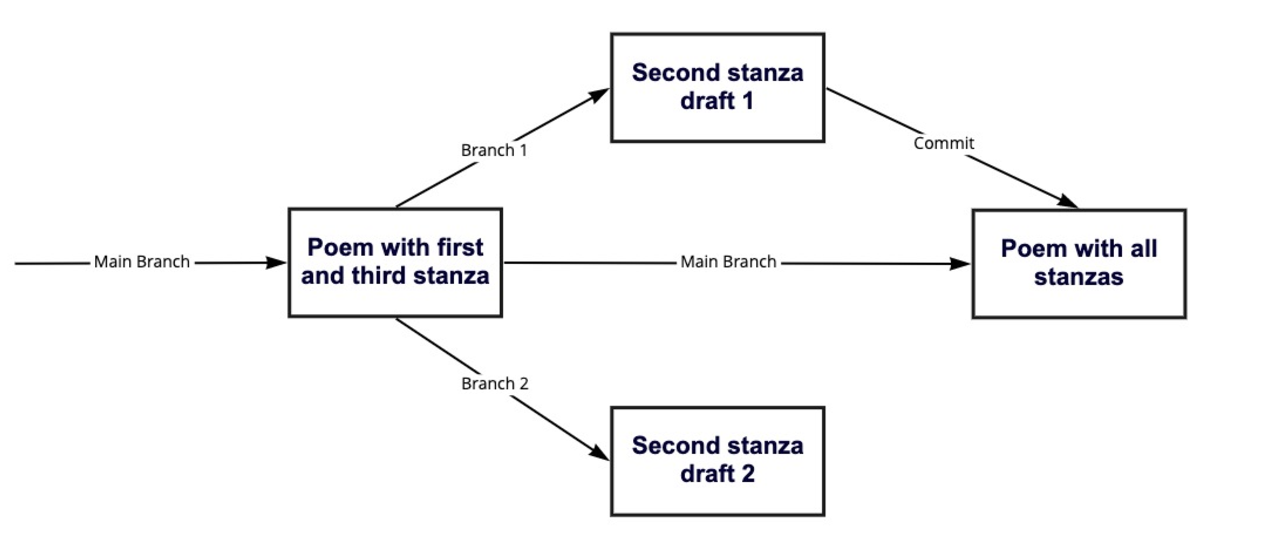
\includegraphics[width=\linewidth]{external/merge_poem1.pdf}
\end{image}%
\tcblower
\end{figureptx}%
\begin{figureptx}{Figure}{Diagram showing another possible merge into main}{figure-SS_thinkbranch-k}{}%
\begin{image}{0.05}{0.9}{0.05}{}%
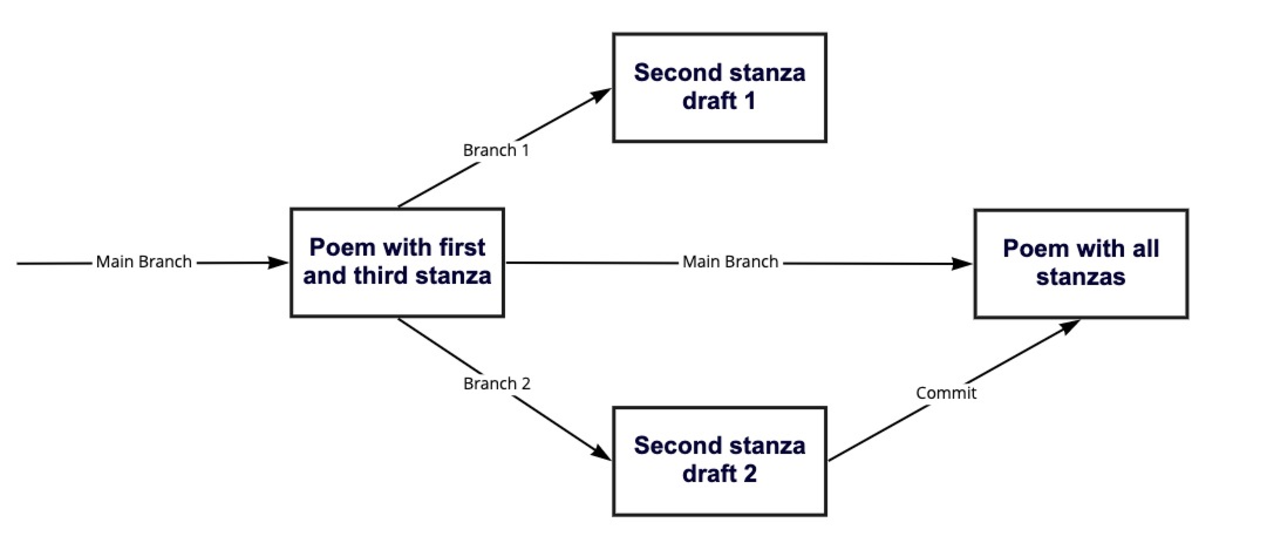
\includegraphics[width=\linewidth]{external/merge_poem2.pdf}
\end{image}%
\tcblower
\end{figureptx}%
You will also often hear about pull requests. Recall how GitHub allows anyone to edit anyone else's code, but in order to change the official version, they have to ask for permission. The asking for permission is sending a pull request. You are asking the creator of the main branch their permission to pull in your changes. Don't worry too much about this now; we will cover it when we get to multi-person collaboration. You will see the term come up in this chapter however which is why I chose to introduce it here.%
\end{subsectionptx}
%
%
\typeout{************************************************}
\typeout{Subsection 3.3.2 Creating a Branch}
\typeout{************************************************}
%
\begin{subsectionptx}{Subsection}{Creating a Branch}{}{Creating a Branch}{}{}{subsection-SS_makebranch}
\index{github!branches}%
\index{branches!create}%
Creating a branch is not difficult. To do so, first make sure you are on the ``Code'' tab of your repository titled \mono{aboutme}. Below the list of tabs, you should have a row of items. The first is a button with a branch-like icon with the word ``main''. Next to that, there is the same branch-like icon with ``1 branch'' and then a tag-like icon with ``0 tags'' (\hyperref[figure-fig-hub-new-branch]{Figure~{\xreffont\ref{figure-fig-hub-new-branch}}}). \footnote{Your numbers may be different if you played around with GitHub before this step.\label{fn-SS_makebranch-d-g}} Now,%
\begin{enumerate}
\item{}Click on the word ``main''. This will open a drop-down menu with all of your current branches (\hyperref[figure-fig-hub-new-branch]{Figure~{\xreffont\ref{figure-fig-hub-new-branch}}}). You probably only have one branch: the main branch.%
\item{}We will be adding a part to our README file: our favorite animal. Type \mono{animal} in to the textbox that appears. Your cursor should navigate there automatically.%
\item{}Since we don't have a branch named \mono{animal}, GitHub asks us if we want to create a new branch with that name. That is indeed what we want to do. Click on ``Create branch: animal from 'main'''%
\end{enumerate}
%
\begin{figureptx}{Figure}{Reference for creating a new branch on GitHub}{figure-fig-hub-new-branch}{}%
\begin{sidebyside}{2}{0}{0}{0}%
\begin{sbspanel}{0.5}%
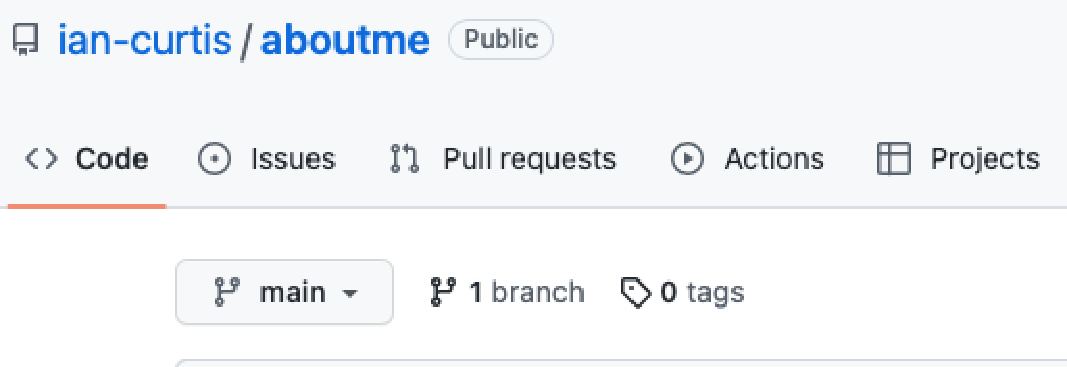
\includegraphics[width=\linewidth]{external/hub_new_branch.pdf}
\end{sbspanel}%
\begin{sbspanel}{0.5}%
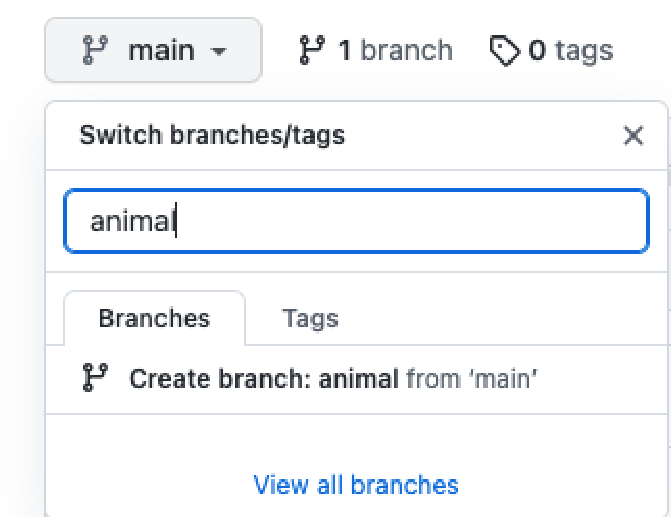
\includegraphics[width=\linewidth]{external/hub_new_branch_animal.pdf}
\end{sbspanel}%
\end{sidebyside}%
\tcblower
\end{figureptx}%
Once you have created the new branch \mono{animal}, your screen will have changed slightly. The branch-like icon with the word ``main'' has changed to say ``animal''. This is how you will know what branch you are looking at. Also notice how it says we have ``2 branches''. We do: main and animal. Right underneath those items, you may also notice GitHub has placed a box stating that ``This branch is up to date with main.''. This is what we should expect. This statement indicates that the \mono{main} branch and the \mono{animal} branch are identical (see \hyperref[figure-fig-hub-animal-initial]{Figure~{\xreffont\ref{figure-fig-hub-animal-initial}}}).%
\begin{figureptx}{Figure}{Diagram mapping branches after creating the animal branch}{figure-fig-hub-animal-initial}{}%
\begin{image}{0.15}{0.7}{0.15}{}%
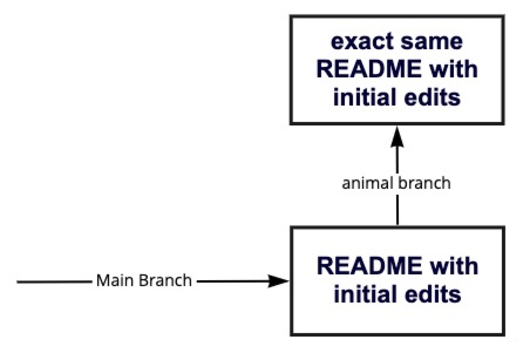
\includegraphics[width=\linewidth]{external/hub_animal_initial.pdf}
\end{image}%
\tcblower
\end{figureptx}%
\begin{assemblage}{Assemblage}{A Few Notes on Branches.}{assemblage-branchnotes}%
%
\begin{itemize}[label=\textbullet]
\item{}Take caution when naming branches. You should follow the same guidelines the were discussed with file and folder names in \hyperref[section-S_filenames]{Section~{\xreffont\ref{section-S_filenames}}}.%
\item{}Branch names should be extremely descriptive in the shortest way possible. It is wise to break up your project into distinct chunks and assign one branch for each chunk.%
\item{}It is very easy to get lost within branches. You can create sub-branches off of normal branches. You can delete branches or ignore them. I advise only creating the branches you need at the current moment. If sub-branches (i.e., sub-tasks) are something you are interested in working with, I would recommend keeping a picture of the relationship between branches.%
\item{}Once you are done with a branch, delete it. Otherwise, it will clog up your branch list. You can always create it again.%
\end{itemize}
%
\end{assemblage}
\end{subsectionptx}
%
%
\typeout{************************************************}
\typeout{Subsection 3.3.3 Working On a Branch}
\typeout{************************************************}
%
\begin{subsectionptx}{Subsection}{Working On a Branch}{}{Working On a Branch}{}{}{subsection-SS_workingbranch}
\index{branches!edit}%
We named the new branch \mono{animal} to describe the changes we plan to make: add our favorite animal. Editing a file on a branch is no different than editing a file on \mono{main}. However, we now have a safeguard. We can edit and commit as much as we want to the \mono{animal} branch and never make any changes to \mono{main}. Returning to the analogy at the beginning of the section, we no longer have to write in pen on fancy paper unless we are sure we want to change something.%
\par
Hopefully you are able to see the power in this. In a more serious project, commiting too early could have much bigger ramifications. Suppose I am coding a new character for a video game and the character has to use vulgar language. In a simple workflow, I would create a branch called \mono{vulgar} or \mono{new\_npc} with a sub-branch of \mono{language}. Then, I would incorporate my code on my branches. Once that was done, I would run my code to test that it worked. Then I would submit a pull request, requesting my boss to pull in my new changes into the official version of the game. They would likely take a look at my code and try it themselves before accepting the changes. But let's say I forgot to add in the censorship beep over the language. If I had just merged right into main, my mistake may have been missed and I could get in serious trouble. But since I worked on a branch, my forgetfulness can be caught before the changes get incorporated and there won't be any flustering to quickly revert changes or fix the error.%
\begin{inlineexercise}{Checkpoint}{Editing a File On a Branch.}{exercise-editbranch}%
You should already have a README file in your repo from the activities in \hyperref[subsection-hub-editfile]{Editing a File}. Now, head back to the file to edit it and add a level two heading called ``My Favorite Animal''. Underneath that, type your favorite animal. Do not commit yet.%
\par
The current state of the branch is shown in \hyperref[figure-fig-hub-animal-edit]{Figure~{\xreffont\ref{figure-fig-hub-animal-edit}}}.%
\end{inlineexercise}%
\begin{figureptx}{Figure}{Diagram showing branches after add a favorite animal}{figure-fig-hub-animal-edit}{}%
\begin{image}{0}{1}{0}{}%
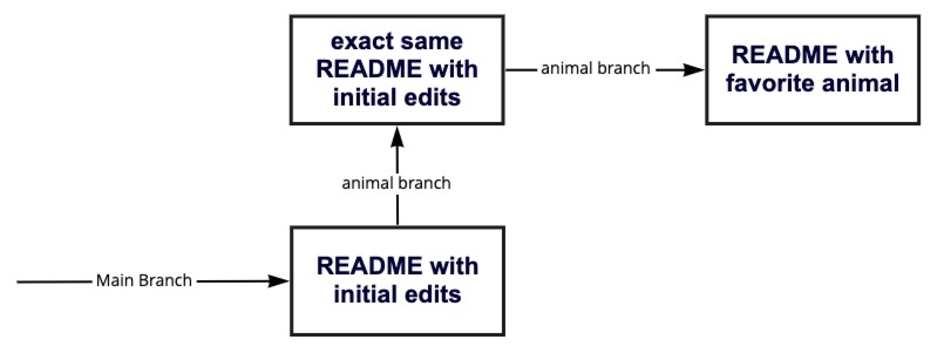
\includegraphics[width=\linewidth]{external/hub_animal_edit.pdf}
\end{image}%
\tcblower
\end{figureptx}%
\index{commit message}\index{message|see{commit message}}\index{github!commit message} After you have made some changes, head to the ``Commit changes'' dialog (top right). Now, it is time to introduce commit messages. A \terminology{commit message} is a short, but informative (notice a recurring pattern?) note of what your changes do. You may be tempted to skip this when working with yourself. Please try to write the best commit messages \emph{at all times}. When you look back at your repo in the future, it will be helpful for you to remember what you did. Commit messages also help others who may look at your project know what you did in each commit. You may see my various branch names and commit messages at \href{https://github.com/ian-curtis/gitstarted/commits/main}{the commit list for this book on GitHub}\footnote{\nolinkurl{github.com/ian-curtis/gitstarted/commits/main}\label{fn-SS_workingbranch-g-h}}.%
\par
Let's create a commit message for our changes on the \mono{animal} branch. In the ``Commit changes'' dialog, there is a text box that is autofilled with ``Update README.md''. This is the default and for some instances may be enough. But I have the tendency to write slightly more detailed messages for my commits and I recommend you do so as well. Instead, type ``add favorite animal''. There is no need to add the file name as this message will only be tied to the file(s) you have edited. (Later on, we will see that specific commit messages are only associated with the files you have staged and committed but that's a topic for \hyperref[chapter-C_gitsolo]{Chapter~{\xreffont\ref{chapter-C_gitsolo}}}.)%
\begin{assemblage}{Assemblage}{A Note On Commit Messages.}{assemblage-commitmessages}%
It is up to you how to format your message. Some people write in complete sentences while others use incomplete sentences with capital letters. Some people use past tense, others present tense, and even others use present participles (add\emph{ing}). I choose to use present tense with incomplete sentences and lowercase letters. But that's my preference. You should find what you like and stick with it.%
\par
\textellipsis{}Except when you're editing someone else's files. In this case, pay attention to how someone else words their commit messages and imitate them. This will make life easier for the owner of the files and for anyone else who looks at the files in the future. You may even find that your commit message is changed by the owner of a repository to match their guidelines.%
\end{assemblage}
It is not necessary to fill out the description text box (feel free to do so if you would like!). Ensure the ``Commit directly to the \mono{animal} branch.'' is selected, then click ``Commit changes''.Your file should be updated! Just remember, \emph{you have only updated the copy of the file on the \mono{animal} branch, not \mono{main}}.%
\par
Navigate back to the code tab to continue. Make sure you are still on the \mono{animal} branch. You can verify this by looking at the drop-down menu text or by checking the contents of your README file (if your favorite animal is there, you are on the \mono{animal} branch).%
\begin{figureptx}{Figure}{Diagram showing our commit from \mono{animal} to \mono{animal}}{figure-fig-hub-animal-commit}{}%
\begin{image}{0.05}{0.9}{0.05}{}%
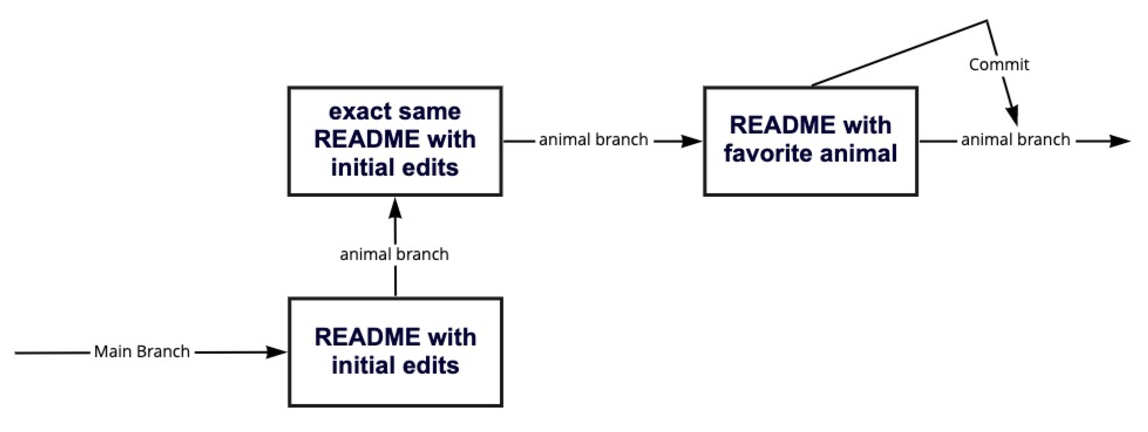
\includegraphics[width=\linewidth]{external/hub_animal_commit.pdf}
\end{image}%
\tcblower
\end{figureptx}%
\end{subsectionptx}
%
%
\typeout{************************************************}
\typeout{Subsection 3.3.4 Creating a Pull Request (with Yourself)}
\typeout{************************************************}
%
\begin{subsectionptx}{Subsection}{Creating a Pull Request (with Yourself)}{}{Creating a Pull Request (with Yourself)}{}{}{subsection-SS_pullrequest}
\index{pull request}%
\index{github!pull request}%
\index{merge}%
\index{github!merge}%
Alright, so you've edited a file on a branch AND you are happy with your changes. Everything looks good and works well on the branch so you are ready to incorporate your changes into the official version of your project. This is called creating a \terminology{pull request}. It may sound odd to call it a pull request when it seems like you are actually \emph{pushing} your changes toward the main branch. However, in cases where you don't have permission to access the main branch of another repo, so you have to request that someone \emph{pull} your changes into the main branch.%
\par
I admit, it is silly to have to work with pull requests when working solo. Why would I need to ask myself permission to pull in my own changes? But pull requests are essential when working with multiple collaborators and I recommend using branches and pull requests in your own individual work for practice, good habits, and safeguards against code failures.%
\par
\index{commit!ahead and behind} Pull requests are only necessary when using branches (recall how when we edited the README file directly from the main branch we had no pull requests). We are currently in a situation that would require a pull request. How do we create one? First notice (on your GitHub repository for the \mono{animal} branch) how a new message has appeared. This probably says%
\begin{quote}%
This branch is 1 commit ahead of main.%
\end{quote}
\begin{figureptx}{Figure}{The GitHub commits summary box}{figure-fig-hub-commit-ahead}{}%
\begin{image}{0.05}{0.9}{0.05}{}%

\includegraphics[width=\linewidth]{external/hub_commit_ahead.pdf}
\end{image}%
\tcblower
\end{figureptx}%
... as seen in \hyperref[figure-fig-hub-commit-ahead]{Figure~{\xreffont\ref{figure-fig-hub-commit-ahead}}}. This is GitHub's way of telling you that the branch you are currently on has changes that are not reflected on the main branch. Specifically, we have committed one time and the changes from that single commit do not appear on main. We could go and edit the README file some more and commit those changes. In that case, we would be 2 commits ahead of main.%
\par
The dialog box that contains this message also has another feature: a ``Contribute'' option (\hyperref[figure-fig-hub-contribute]{Figure~{\xreffont\ref{figure-fig-hub-contribute}}}). If you click on this option, a box pops up telling us again that we are 1 commit ahead of main. Here, there is a button inviting us to ``Open pull request''. Click on this.%
\begin{figureptx}{Figure}{The contribute dialog box.}{figure-fig-hub-contribute}{}%
\begin{image}{0.25}{0.5}{0.25}{}%
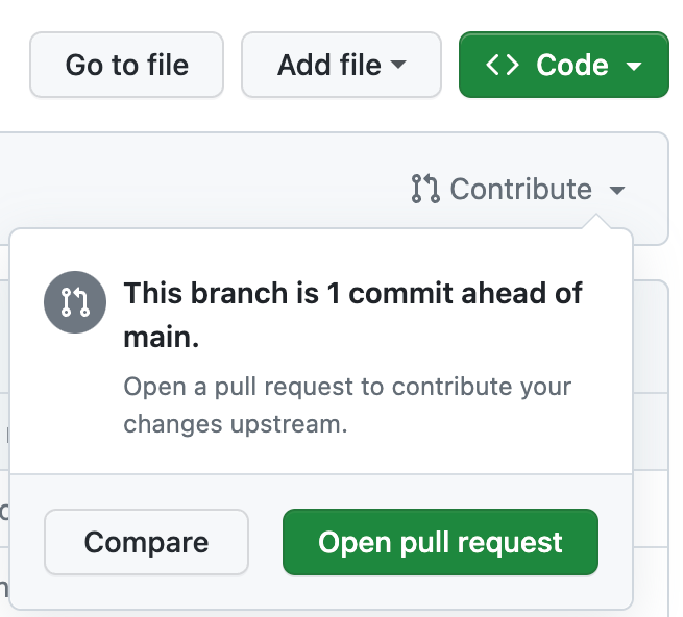
\includegraphics[width=\linewidth]{external/hub_contribute.pdf}
\end{image}%
\tcblower
\end{figureptx}%
There is a lot on this page but most of it will be dealt with later. For right now, notice that GitHub tells us which branch we are trying to send to main at the top. \mono{animal} should be on the right and is pointing towards \mono{main} (see \hyperref[figure-fig-hub-able-merge]{Figure~{\xreffont\ref{figure-fig-hub-able-merge}}}). Next to this, you should see a check mark and an ``Able to merge'' message. This is good; see \hyperref[section-S_mergeconflict]{Section~{\xreffont\ref{section-S_mergeconflict}}} if your branches cannot be automatically merged.%
\begin{figureptx}{Figure}{Branch selection drop-down menus and able to merge confirmation.}{figure-fig-hub-able-merge}{}%
\begin{image}{0.1}{0.8}{0.1}{}%
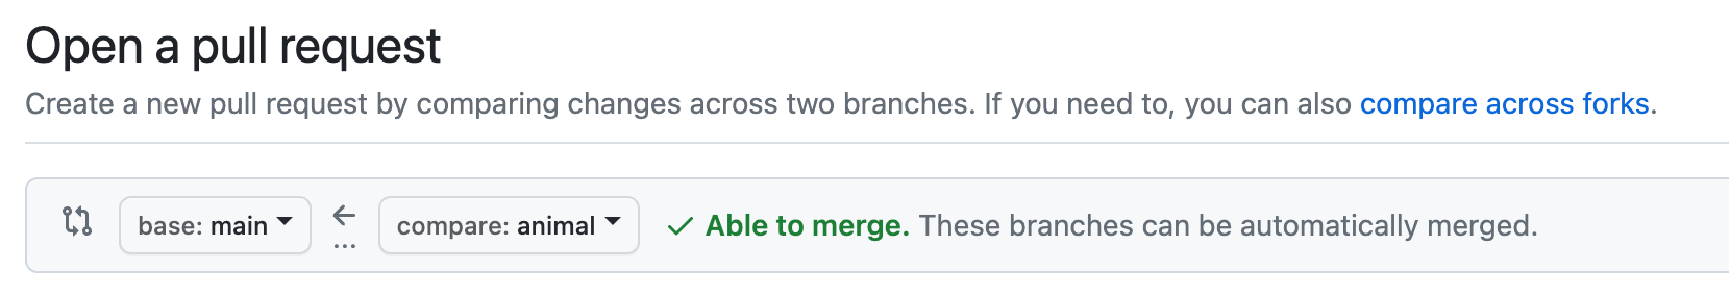
\includegraphics[width=\linewidth]{external/hub_able_merge.pdf}
\end{image}%
\tcblower
\end{figureptx}%
Your cursor should have automatically navigated to a dialog box. This has defaulted to our latest commit message. You should make sure that you have put an informative message on what your pull request accomplishes as a whole. Remember, it is possible to have multiple commits before opening a pull request so you could have adjusted a few things. For us, ``add favorite animal'' is sufficient and we can open the pull request. Click on the ``Create pull request'' button.%
\par
Nice, another new screen. This time notice how we have changed tabs. We are now in the ``Pull requests'' area (and not the Code tab), which should make sense. The pull requests page is for more than just accpeting pull requests. If someone else has contributed to your repo and has opened a pull request, you can start a conversation here. Suppose you have a question about someone's changes or think they should improve their addition before you approve it. You can say that here.%
\par
But we have no problems with ourselves. Our pull request has been created and is waiting for permission to be pulled into main. In some instances, you will have to wait for a repo owner to accept your pull request. However, you are the repo owner and can \terminology{merge} the changes yourself. You can do this on the current screen. Find the ``Merge pull request'' button (\hyperref[figure-fig-hub-no-conflicts]{Figure~{\xreffont\ref{figure-fig-hub-no-conflicts}}}). GitHub will give you the chance to edit the message if necessary. Since we have no changes to make, click on ``Confirm merge''.%
\begin{figureptx}{Figure}{The merge pull request dialog box.}{figure-fig-hub-no-conflicts}{}%
\begin{image}{0.05}{0.9}{0.05}{}%
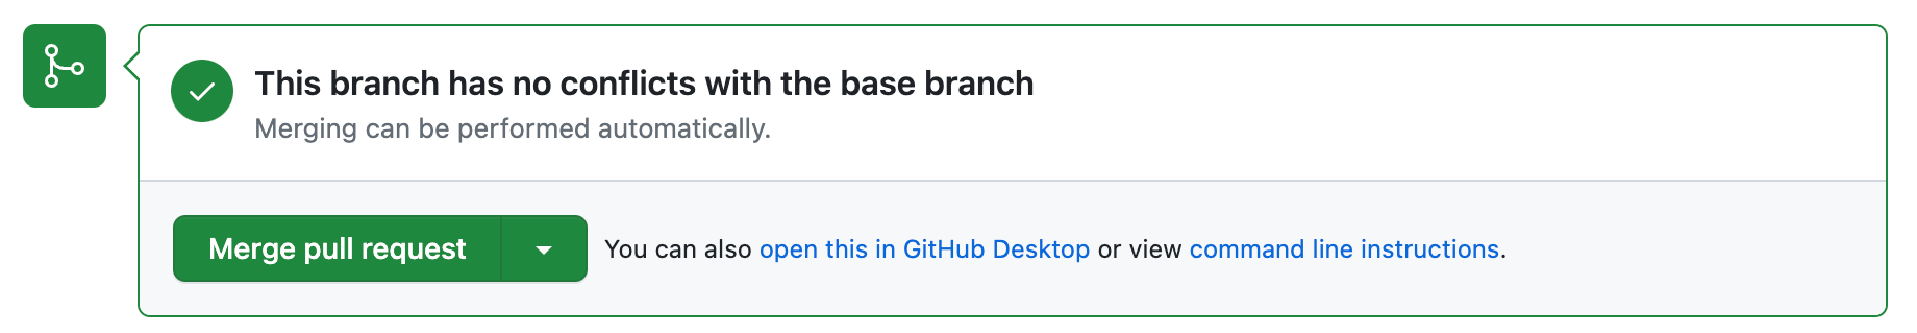
\includegraphics[width=\linewidth]{external/hub_no_conflicts.pdf}
\end{image}%
\tcblower
\end{figureptx}%
Hopefully you were given the ``Pull request successfully merged and closed'' message. From here, click on ``Delete branch''. You should have no fear about deleting the branch at this point. Your changes will not be lost because you just incorporated them into \mono{main}. You now have two identical copies of the same files and can get rid of the extraneous copy: your old branch. If it makes you feel better, GitHub keeps track of commits and merges. If you ever want to revert back to an old version, you can in \hyperref[section-S_hub_revert_commit]{Section~{\xreffont\ref{section-S_hub_revert_commit}}}. For now, go back to the ``Code'' tab and verify that your favorite animal appears in the README in the main branch.%
\begin{figureptx}{Figure}{Diagram showing a pull request from \mono{animal} to \mono{main}}{figure-fig-hub-animal-merge}{}%
\begin{image}{0.05}{0.9}{0.05}{}%
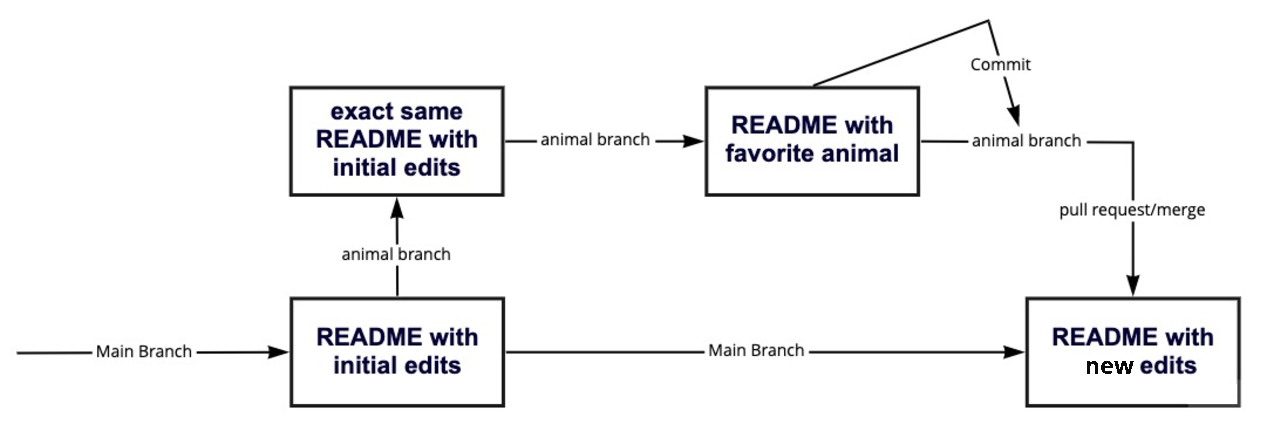
\includegraphics[width=\linewidth]{external/hub_animal_merge.pdf}
\end{image}%
\tcblower
\end{figureptx}%
\begin{inlineexercise}{Checkpoint}{Branches and Pull Requests.}{exercise-solo-branch-pr}%
It is time to put together what you learned in this section and make some edits of your own. Don't be afraid to look back at what we did earlier for reassurance. Start this exercise on the ``Code'' tab of your \mono{aboutme} repo. The goal of this exercise is to add another section to the README file by creating a branch, making edits, and opening a pull request.%
\begin{enumerate}[font=\bfseries,label=(\alph*),ref=\alph*]%
\item{}Think about something about you that you have not put in the README yet. Perhaps your favorite food, quote, or historical character. Once you have chosen what you want to add, create a branch with an appropriate name.%
\item{}Edit your README file. You should have at the very least a new level two heading indicating what you are adding and a piece of text with your addition.%
\item{}Add an approporiate commit message and commit your changes to your new branch.%
\item{}Open a pull request to merge your changes into the main branch.%
\item{}Merge your new pull request into main and delete your old branch.%
\item{}Verify that your change did in fact get merged into main.%
\end{enumerate}%
\end{inlineexercise}%
\end{subsectionptx}
\begin{conclusion}{}%
Congratulations! Hopefully you have a better understanding of how branches and pull requests work in GitHub (and their potential).%
\end{conclusion}%
\end{sectionptx}
\end{chapterptx}
 %
%
\typeout{************************************************}
\typeout{Chapter 4 Git Solo}
\typeout{************************************************}
%
\begin{chapterptx}{Chapter}{Git Solo}{}{Git Solo}{}{}{chapter-C_gitsolo}
\renewcommand*{\chaptername}{Chapter}
\index{version control}%
\index{git}%
\begin{introduction}{}%
Git is difficult to wrap your head around partly because it's new and partly because it's scary. There are many things that could go wrong and that are difficult (but usually not impossible) to revert. But Git's power of version control is so important. The goal of this chapter is to help you get familiar with working with Git on the command line and how it interacts with GitHub.%
\par
I assume you have read \hyperref[chapter-C_commandline]{Chapter~{\xreffont\ref{chapter-C_commandline}}} and \hyperref[chapter-C_githubsolo]{Chapter~{\xreffont\ref{chapter-C_githubsolo}}} before tackling this chapter. The vocabulary used by GitHub is identical to Git's (this is on purpose) and if you understand the basics of how Github operates, you will find some of Git to be simple. Git runs on the command line so it is also important to have some experience with a terminal and how it operates.%
\par
I also assume you have followed along with the GitHub activities throughout \hyperref[chapter-C_githubsolo]{Chapter~{\xreffont\ref{chapter-C_githubsolo}}}. They are super important for understanding the content and I continue where I left off in this chapter. We will be updating the \mono{aboutme} repository with Git rather than just GitHub.%
\end{introduction}%
%
%
\typeout{************************************************}
\typeout{Section 4.1 Getting Set Up with Git}
\typeout{************************************************}
%
\begin{sectionptx}{Section}{Getting Set Up with Git}{}{Getting Set Up with Git}{}{}{section-S_gitsetup}
\index{git}%
\index{git!setup}%
\begin{introduction}{}%
You should have Git installed at this point. If not, see \hyperref[preface-materials-windows]{Materials: Windows}, \hyperref[preface-materials-mac]{Materials: Mac}, or \hyperref[preface-materials-linux]{Materials: Linux}. This means you already have Git ready to go. But how do we use it? We created a repo on GitHub but need a way to connect that repo with our personal computer. That's a great feature of Git: \emph{to connect the files on your computer to GitHub.} It also performs version control and automatically records changes that have been committed.%
\par
It's not always feasible to edit file on GitHub, as we did in \hyperref[section-S_hubfirstrepo]{Section~{\xreffont\ref{section-S_hubfirstrepo}}} and \hyperref[section-S_hubbranches]{Section~{\xreffont\ref{section-S_hubbranches}}}. Certain text editors (for instance, Visual Studio Code which you might also have installed) have features built in to ease coding and file editing. \initialism{VS} Code extensions might add color to text to help you see what's going on in your code. Others provide bug fixing and error catching before the errors actually occur. In general, you will edit files on your personal computer and will want to share them with the world. \emph{I would stay away from editing on GitHub unless you have a small correction and\slash{}or you don't need any special editing tools.}%
\end{introduction}%
%
%
\typeout{************************************************}
\typeout{Subsection 4.1.1 Cloning a Repository}
\typeout{************************************************}
%
\begin{subsectionptx}{Subsection}{Cloning a Repository}{}{Cloning a Repository}{}{}{subsection-SS_cloning}
\index{clone}%
\index{repository!cloning}%
\index{local}%
\index{editing locally}%
\index{git!clone}%
In order to make Git work, we need to set up a connection between your computer and your GitHub repo. From here on, I might refer to your personal files as your \terminology{local files}. A file is typically considered ``local'' if it does not exist on GitHub (or anywhere else on the internet). It is local because only you have access to it. You will likely hear other people use this term and its derivatives (such as ``editing locally''). Whenever it comes up, it refers to work\slash{}files\slash{}things on your computer and not online.%
\par
So let's use the new vocab. We need a way to edit our GitHub repo locally but still have version control and GitHub tools. Git is the right tool for the job. Performing this connection is called cloning. A \terminology{clone} of a repository is a local version of a repo that exists on GitHub. Luckily for us, GitHub expects us to do this and makes it rather simple to do.%
\par
Somewhat unfortunately, one thing must be done before we are able to clone a repo. Interacting with your GitHub materials in this way will require authentication; in other words, your password. This is necessary for safety and is a smart feature. However, Git\slash{}GitHub has deprecated the use of passwords on the command line so we must generate an Personal Access Token (\acronym{PAT}). The following procedure guides you through this process. I recommend creating a new \acronym{PAT} for each repo to ensure that if anyone gets unauthorized access of one repo, they won't be able to get to your others.%
\begin{project}{Git Procedure}{Generating a \acronymintitle{PAT}.}{project-gitproc-pat}%
\index{github!\acronym{PAT}}%
\begin{enumerate}[font=\bfseries,label=(\alph*),ref=\alph*]%
\item{}Click on your GitHub profile icon and navigate to Settings.%
\item{}Scroll down and click on ``Developer Settings''.%
\item{}Click on ``Personal access tokens'' and then ``Tokens (classic)''. This page will give you an overview of all the tokens you have created, their expiration dates, and the things they have access to.%
\item{}Click on ``Generate new token'' and then ``Generate new token (classic)''. Your GitHub password may be required.%
\item{}Enter a title for your token. What is your project? This name doesn't really matter; it exists solely to help you remember why you made it. If this is your first \acronym{PAT}, perhaps name it ``Git Started Work'' or ``About Me''.%
\par
If you choose the above, make sure you only use the token for that purpose!%
\item{}Choose an expiration date. At what point do you plan on being done with this project? Set the date for a month after that. Don't fret too much about it; you can always create a new \acronym{PAT} later for the same project. But I can bet that you won't want to do this process more than once for one project if you can help it.%
\item{}Select a scope or scopes. What do you want this \acronym{PAT} to give you access to? This will depend on your project but less is better (for privacy and security). If you do not give a \acronym{PAT} permission to do something, that something will not be able to be done locally, even by you.%
\par
For this project, you will want the ``repo'' scope and maybe the ``user'' scope. Once you have the scope(s) selected, click ``Generate token''.%
\item{}You will get an email that a \acronym{PAT} was created. Record your \acronym{PAT} somewhere. You will never see it again after you close or refresh the page. Don't put it somewhere easily accessible. \emph{Treat \acronym{PAT}s like passwords.} They are confidential and should not be shared. When Git (on the command line) asks for your password, you will enter in your \acronym{PAT} instead.%
\end{enumerate}%
\end{project}%
Now that we have a \acronym{PAT}, let's work on cloning a repo! You will likely need your \acronym{PAT} in this procedure. Note that sometimes Git remembers old \acronym{PAT}s. If Git does not ask you for a password, this doesn't mean something went wrong, it just means that you are already authenticated.%
\begin{project}{Git Procedure}{Cloning from GitHub.}{project-try-git-clone}%
\index{git!clone}%
This procedure assumes you have a repo on GitHub called \mono{aboutme} and have been following along with the changes as described in \hyperref[chapter-C_githubsolo]{Chapter~{\xreffont\ref{chapter-C_githubsolo}}}.%
\begin{enumerate}[font=\bfseries,label=(\alph*),ref=\alph*]%
\item{}Navigate to the Code tab your repo \mono{aboutme}. Make sure you are on the main branch.%
\item\label{task-clone-https}Find the dialog box labeled ``Code'' (yes, the Code box inside the Code tab). This can be found above your list of files.%
\par
Click on this Code box and make sure you have the ``Local'' sub tab selected. This part is titled ``Clone'' which is a good sign. A url-like string should appear (if not, be sure you have the HTTPS tab selected.) Copy this string.%
\par
See \hyperref[figure-fig-hub-clone-box]{Figure~{\xreffont\ref{figure-fig-hub-clone-box}}} for what the Code submenu might look like.%
\begin{figureptx}{Figure}{The cloning dialog box on GitHub}{figure-fig-hub-clone-box}{}%
\begin{image}{0.2}{0.6}{0.2}{}%
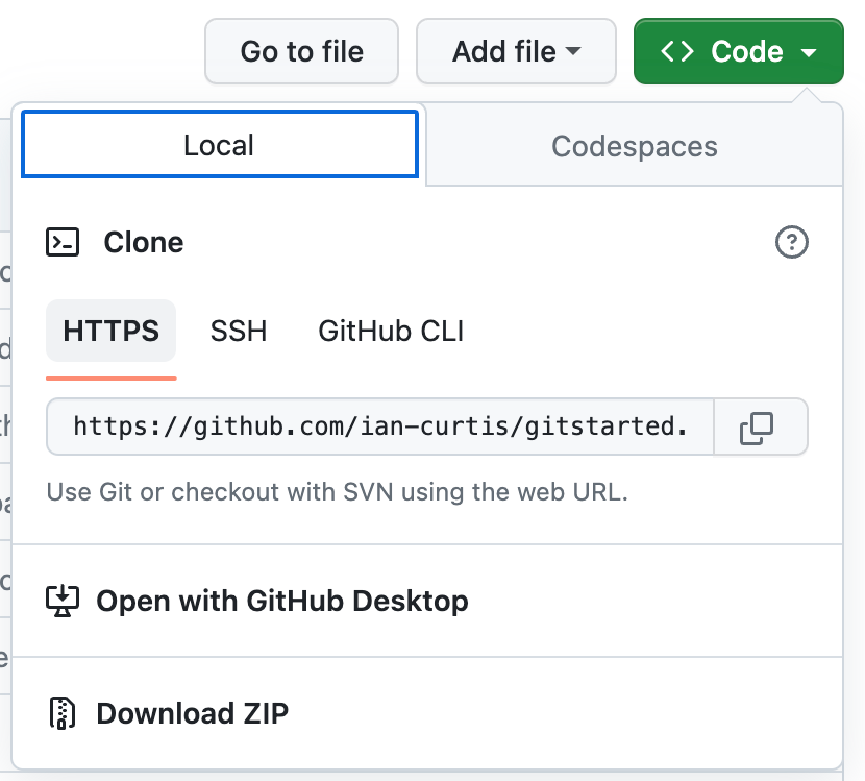
\includegraphics[width=\linewidth]{external/hub_clone_box.pdf}
\end{image}%
\tcblower
\end{figureptx}%
\item{}Open your terminal. Use \mono{cd} to navigate to a folder where you want your repo to live locally. Remember that repositories are essentially folders. When you clone your repo, it will look like a folder on your computer. In some cases, it might not make sense to create a folder and then clone your repo as it will look like a folder that contains a folder. Note that the name of the cloned repo\slash{}folder will be the name of your repository.%
\item{}You should be at the location you want your repo to be. It is now time to activate Git. Every time you use a Git command, you start with \mono{git}, then the command. For cloning:%
\begin{console}{0}{1}{0}
> (*\consoleinput{git clone <copied-https-string>}*)
Cloning into 'aboutme'...
remote: Enumerating objects: 17, done.
remote: Counting objects: 100% (14/14), done.
remote: Compressing objects: 100% (9/9), done.
remote: Total 17 (delta 2), reused 0 (delta 0), pack-reused 3
Receiving objects: 100% (17/17), 5.06 KiB | 1.01 MiB/s, done.
Resolving deltas: 100% (2/2), done.
\end{console}
where \textless{}copied-https-string\textgreater{} is replaced with the HTTPS string you copied in \hyperref[task-clone-https]{Task~{\xreffont\ref{project-try-git-clone}}.{\xreffont\ref{task-clone-https}}}. Press \kbd{Enter} to run the command.%
\par
Your terminal may ask you for your GitHub username and password. This is ok: enter your username and instead of typing your normal GitHub password, paste\slash{}type your \acronym{PAT} as found in \hyperref[project-gitproc-pat]{Git Procedure~{\xreffont\ref{project-gitproc-pat}}}.%
\item{}Verify that the clone worked. In the location you chose (on your computer), you should see a new folder with the name of your repository. Inside of that folder will be your files!%
\end{enumerate}%
\end{project}%
\emph{Cloning a repository does not navigate you into that repo.} In other words, when you clone a repo, you won't see the files in the repo until you \mono{cd} into the newly-created directory. In order to use Git, you will have to navigate your terminal into the repo. In this instance, you would do \mono{cd aboutme}.%
\end{subsectionptx}
%
%
\typeout{************************************************}
\typeout{Subsection 4.1.2 Branches With Git}
\typeout{************************************************}
%
\begin{subsectionptx}{Subsection}{Branches With Git}{}{Branches With Git}{}{}{subsection-SS_gitbranches}
\index{git!branches}%
\index{branches!switch}%
Great! We've cloned a repository. Now what? You probably want to jump into editing files but wait! Best practice says to create a new branch first. Sure, you are working solo (if you aren't, see \hyperref[part-part-collab]{Part~{\xreffont\ref{part-part-collab}}}) and you can really do what ever you want. You could just edit everything on the main branch and never have to worry about other branches. No one will be able to screw with your files without permission.%
\par
No one except you! Yes, you could make a mistake and break your program or project. You want to avoid that. I would recommend \emph{always} using branches whether you are working alone or not. If you make a horrible mistake, branches help you fix mistakes without messing with your main branch. Remember, if your repo is public, anyone can access it. Anyone can view the files, download the files, clone your repo, or fork your repo (\hyperref[subsection-SS_forking]{Subsection~{\xreffont\ref{subsection-SS_forking}}}). You want to make sure that the files on the main branch are up-to-date AND functional at all times. Branches will let you test new things without breaking main.%
\par
We saw earlier how to work with branches on GitHub, but you can also do this right from the command line. This can be done with two commands (or one, see \hyperlink{paragraphs-branch-shortcut}{Branch\slash{}Checkout Shortcut}) and doesn't involve navigating multiple pages as we did on GitHub (\hyperref[section-S_hubbranches]{Section~{\xreffont\ref{section-S_hubbranches}}}).%
\begin{project}{Git Procedure}{Branches With Git.}{project-gitproc-branches}%
\index{git!branches}%
\index{git!switch}%
\index{git!checkout}%
Later on in this chapter, you will be adding to your README file. You first will add the country you were born in.%
\begin{enumerate}[font=\bfseries,label=(\alph*),ref=\alph*]%
\item{}Ensure that your terminal is navigated into your repo. You may have noticed that your terminal changed! The name of your active branch is displayed by the file path. Mine now has a \mono{(main)}. This is how you remember which branch you are editing on.%
\item{}Remember that each Git command begins with \mono{git} to let your computer know you will be using Git. To create a new branch, use the following:%
\begin{console}{0}{1}{0}
> (*\consoleinput{git branch <branch-name>}*)
\end{console}
where \mono{<branch-name>} is the non-spaced name of your new branch. Try creating a new branch now, with the name of \mono{country}. So,%
\begin{console}{0}{1}{0}
> (*\consoleinput{git branch country}*)
\end{console}
\item{}Well, shoot. Git still says we're on the main branch. We want it to tell us that we are on the \mono{country} branch. That's because we need to tell Git that we want to work on that new branch. Git doesn't move you to that branch in case you want to make more than one branch at one time.%
\par
With Git, navigating to a new branch is done with the \mono{switch} command. In general,%
\begin{console}{0}{1}{0}
> (*\consoleinput{git switch <branch-name>}*)
Switched to branch '<branch-name>'
\end{console}
If done correctly, Git will tell you that it switched to the new branch. This should be reflected in the branch name indicator. Switch to your new branch \mono{country}:%
\begin{console}{0}{1}{0}
> (*\consoleinput{git switch country}*)
Switched to branch 'country'
\end{console}
My terminal now says \mono{(country)} instead of \mono{(main)} so I have verification that the process worked.%
\end{enumerate}%
\end{project}%
\begin{paragraphs}{Branch\slash{}Checkout Shortcut.}{paragraphs-branch-shortcut}%
Using a little terminal trick, we can actually create a branch and switch to that branch at the same time. This uses the \mono{-c} argument. For our example in \hyperref[project-gitproc-branches]{Git Procedure~{\xreffont\ref{project-gitproc-branches}}},%
\begin{console}{0}{1}{0}
> (*\consoleinput{git switch -c <branch-name>}*)
Switched to new branch '<branch-name>'
\end{console}
By adding the \mono{-c} argument to the \mono{switch} command, Git creates a new branch with the title given and checks out that branch. This is quite useful if you are only creating one branch and want to switch right to it. If you are uncomfortable with this, then feel free to continue using the method in \hyperref[project-gitproc-branches]{Git Procedure~{\xreffont\ref{project-gitproc-branches}}}. Each will get you to the same place.%
\end{paragraphs}%
\begin{paragraphs}{Note About \mono{git switch} (Optional).}{paragraphs-SS_gitbranches-i}%
The \mono{git switch} command was introduced to help remove user confusion. Previously, the command was \mono{git checkout <branch-name>}. However \mono{checkout} has two functions: to switch branches and to reset files (if a file has edits that you want to restore, you can use \mono{checkout} to restore the file to how it was before you made the changes).%
\par
\mono{git checkout} still exists and you are welcome to use it to switch branches (you would use \mono{git checkout -b <branch-name>}). However, to avoid confusion, I recommend using \mono{git switch} for changing branches and \mono{git restore} for restoring files.%
\end{paragraphs}%
\end{subsectionptx}
\begin{conclusion}{}%
You are now ready to edit files! You determined a chunk of your project to start with (adding your birth country), created a corresponding branch (\mono{country}) and checked out that branch. Until you change your branch again, all edits will take place on your current branch \emph{only}. Continue on to edit your README file!%
\end{conclusion}%
\end{sectionptx}
%
%
\typeout{************************************************}
\typeout{Section 4.2 Editing Files}
\typeout{************************************************}
%
\begin{sectionptx}{Section}{Editing Files}{}{Editing Files}{}{}{section-S_gitedits}
\index{git!edit}%
\index{edit files}%
\index{files!edit}%
Admittedly, the title of this section is a little misleading. You can't edit files with Git. Git just keeps track of your files and your changes. Take this section as a chance to familiarize yourself with your text editor (\initialism{VS} Code is recommended and is demonstrated here).%
\par
To recap, we used the command line and Git to start the version control process for our next edits. We activated a branch called \mono{country} which we chose intentionally because we plan on adding our country to the README file. Git will keep the \mono{country} branch ``active'' until we tell it to switch to another branch. Any changes you make, files you delete, or files you create will be recorded under this \mono{country} branch. In other words, only the \mono{country} branch will change, not \mono{main}.%
\par
But let's try editing our file. This is the main goal after all. Open your README file in your preferred text editor. If you're feeling adventurous, use the terminal to do it. If you are using \initialism{VS} Code, read \hyperref[assemblage-open-file-vscode]{Opening Files With \initialismintitle{VS} Code} before using the terminal to open the file.%
\begin{assemblage}{Assemblage}{Opening Files With \initialismintitle{VS} Code.}{assemblage-open-file-vscode}%
Try to open the README file with the terminal. (Remember how? See \hyperref[section-S_commands]{Section~{\xreffont\ref{section-S_commands}}} if not.) What happened?%
\par
Any number of things could have happened. It might have worked and \initialism{VS} Code opened with your file ready to edit. Maybe it didn't work at all and no applications opened. Maybe your terminal opened up a different app. The problem with the \mono{open} command is that it picks the default application and opens that. For me, by default, all \mono{.md} files open in RStudio. So, I have to specifically tell my terminal that I want \initialism{VS} Code to open the file, not anything else.%
\par
Luckily, \initialism{VS} Code has its own command! Remember how every Git command starts with \mono{git}? Well that same idea holds for many different commands. To open a file in \initialism{VS} Code, type \mono{code <file-name-and-extension>} where \mono{code} stands for \initialism{VS} Code. Now things should work correctly and \initialism{VS} Code should open your file.%
\end{assemblage}
Hopefully, the contents of the file look familiar. Everything should be the same from when we edited it back in GitHub. Take a minute and add a heading called ``My Birth Country'' and type a sentence stating your birth country. (If you don't want that information on the internet, put any country \textellipsis{} maybe your favorite country.) Save your file.%
\par
I would like to point out some helpful features that \initialism{VS} Code has (other text editors will likely have these same features but not in the same places). In the bottom left corner, \initialism{VS} Code displays the name of your current active branch. This is incredibly useful in case you forget what branch you are on (especially if you are working with multiple branches) or if you want to verify that you are working on a branch and not on main. \initialism{VS} Code also displays (on the left side) a list of all of your files and directories that are inside your GitHub repository allowing easy access to any file you might wish to edit.%
\par
All files you currently have open appear as tabs at the top of your screen. You might also have noticed that when you saved your file, the name of your README changed from white to a cheddar color and an M appeared. \initialism{VS} Code has Git integrated inside of it (one of the many benefits). As Git keeps track of your changes, \initialism{VS} Code tells you which files you have \emph{m}odified (M, yellow), \emph{d}eleted (D, red), or created (U, \emph{u}ntracked). If you were to undo \emph{all} of your changes and saved the file again, the M would disappear and the color would go back to white.%
\par
Hopefully editing the file was fairly straightforward. We now have changes that we have made and we want to get those changes back on to GitHub and on the \mono{main} branch. Don't forget that the changes we made in this section are only local and only on the \mono{country} branch. The next section covers how to stage, commit, and push your changes.%
\end{sectionptx}
%
%
\typeout{************************************************}
\typeout{Section 4.3 Sending Changes Back To GitHub: The Three-Step Process}
\typeout{************************************************}
%
\begin{sectionptx}{Section}{Sending Changes Back To GitHub: The Three-Step Process}{}{Sending Changes Back To GitHub: The Three-Step Process}{}{}{section-S_gitfinalize}
\index{three step process}%
\index{git!three step process}%
\begin{introduction}{}%
Ok, great! We have some edits, but how do we let other people see them? Remember that we have been editing locally so nothing new has shown up on GitHub. The goal here is to share the work with the world, so we need a way to send the changes back to GitHub. Luckily, by cloning our repo, we set up a connection between our local repo and our GitHub repo.%
\par
This is a very important section. Each step must be completed in the proper order to avoid Git errors, headaches, and file loss.%
\par
With Git, there are three main steps to sending edits back to GitHub. That may seem like too many but in fact each step serves a different purpose and gives you a little bit of freedom with how you edit on a branch. The three steps are%
\begin{enumerate}
\item{}Staging your files for sending%
\item{}Commiting your changes%
\item{}Pushing your changes to GitHub%
\end{enumerate}
Step 2 may seem familiar. Yep, the \terminology{commit} that happens here is the same as a commit we did earlier!%
\end{introduction}%
%
%
\typeout{************************************************}
\typeout{Subsection 4.3.1 Wait, Which Files Did I Change Again?}
\typeout{************************************************}
%
\begin{subsectionptx}{Subsection}{Wait, Which Files Did I Change Again?}{}{Wait, Which Files Did I Change Again?}{}{}{subsection-SS_git-status}
\index{git!status}%
This happenes often in large projects (and even in smaller projects). You have a branch, you've been working all day editing and creating files, making sure things work. But now it's time to stage the files and you don't remember what files you've edited! You aren't even positive what the file names are. True, \initialism{VS} Code color codes your edited files but you might have folders and subfolders throught your repository and don't really feel like searching through everything to record what files you changed and which of them you want to send to GitHub.%
\par
Luckily, Git has the command for you! With one line in the terminal, you can easily see a list of files you changed, deleted, and added. Let's explore that with our small case.%
\begin{project}{Git Procedure}{Trying \mono{git status}.}{project-try-git-status}%
\index{tracked files}%
\index{untracked files}%
The command you will need is simple: \mono{git status}. The \mono{git} is necessary to tell the computer that we will be using git and the \mono{status} gives the the current status of all of the files in our repository. We might say that it shows all of the files that Git knows about (\terminology{tracked}) and the files that are new since the latest commit (\terminology{untracked}). Open the terminal, verify that you are in the correct directory and on the correct branch and try the command. Did it spit out what you expected?%
\end{project}%
\begin{paragraphs}{A Small Note On \initialismintitle{VS} Code.}{paragraphs-vscode-term}%
It is worth noting that if you are using \initialism{VS} Code, you do not need to navigate back and forth from a terminal window and the text editor. \initialism{VS} Code has a built-in interface to use your terminal. To access this, navigate to the ``Terminal'' heading in the navigation bar at the top of your screen and click on ``New Terminal''. You may also use the keyboard shortcut \kbd{Ctrl} + \kbd{Shift} + \kbd{\textasciigrave{}} (On a Mac, you would still use \kbd{Ctrl} not \kbd{command}.)%
\end{paragraphs}%
\end{subsectionptx}
%
%
\typeout{************************************************}
\typeout{Subsection 4.3.2 Step 1: Staging Files}
\typeout{************************************************}
%
\begin{subsectionptx}{Subsection}{Step 1: Staging Files}{}{Step 1: Staging Files}{}{}{subsection-SS_git-add}
\index{git!add}%
\index{staging}%
\index{files!staging}%
The first step in sending files back to GitHub is to stage your files. Basically, this step is like you saying ``I have edited some files and these are the ones I would like to send to GitHub''. With our small example, this step is a little silly. We only edited one file, of course it's the one we want to send back.%
\par
The magic of staging files, however, lets you choose which files you want to push back. Maybe I'm working on three files at once, but only two are ready to go back to GitHub. Maybe I'm writing a book and I want my editor to be able to see chapters 1-4 but not chapter 5 (which I'm currently working on). At any given time, you can decide which files you want to stage.%
\begin{project}{Git Procedure}{Trying \mono{git add}.}{project-try-git-add}%
All this is great but how do I stage my files? How do I tell Git which files I want to send back?%
\begin{enumerate}[font=\bfseries,label=(\alph*),ref=\alph*]%
\item{}The output from \mono{git status} in \hyperref[project-try-git-status]{Git Procedure~{\xreffont\ref{project-try-git-status}}} actually gives a hint on how to proceed. If you haven't completed \hyperref[project-try-git-status]{Git Procedure~{\xreffont\ref{project-try-git-status}}}, I recommend doing so now.%
\item{}The staging command is done with \mono{git add} and the command is followed by all the files you want to add. There are three cases with this command:%
\begin{descriptionlist}
\begin{dlimedium}{You want to add specific files}{li-try-git-add-d-a-a-b-a}%
Type in each file name and extension individually with a space between each file.%
\end{dlimedium}%
\begin{dlimedium}{You want to add an entire folder of files}{li-try-git-add-d-a-a-b-b}%
Type in the name of the folder followed by a \kbd{/} (e.g.\@, \mono{images/}).%
\end{dlimedium}%
\begin{dlimedium}{You want to add all changed \slash{} created \slash{} deleted files}{li-try-git-add-d-a-a-b-c}%
Type in a single period (\kbd{.}) instead of file names.%
\end{dlimedium}%
\end{descriptionlist}
%
\par
You can run as many or as little \mono{git add} commands as you wish. For instance, you could do \mono{git add images/ my\_file.txt} or you could do \mono{git add images/} and then do \mono{git add my\_file.txt} separately. It's up to you and how comfortable you feel with Git.%
\par
Try now to stage your README file using one of the three cases above.%
\par\smallskip%
\noindent\textbf{\blocktitlefont Hint}.\hypertarget{hint-try-git-add-d-b}{}\quad{}Case 1 or Case 3 will work in this instance.%
\item{}Use \mono{git status} to verify that your staging worked and that you didn't add any extra files on accident (see \hyperref[project-reverse-git-add]{Git Procedure~{\xreffont\ref{project-reverse-git-add}}} if you did).%
\end{enumerate}%
\end{project}%
\end{subsectionptx}
%
%
\typeout{************************************************}
\typeout{Subsection 4.3.3 Step 2: Committing Files}
\typeout{************************************************}
%
\begin{subsectionptx}{Subsection}{Step 2: Committing Files}{}{Step 2: Committing Files}{}{}{subsection-SS_git-commit}
\index{git!commit}%
\index{commit}%
\index{files!commit}%
\index{commit message}%
``Commit'' is a great name for this step in the process. At this point, you are indeed ready to commit to what you have changed and to send your selected files to GitHub.%
\par
Remember committing from \hyperref[section-S_hubbranches]{Section~{\xreffont\ref{section-S_hubbranches}}}? This commit is the same concept as it was before: telling Git\slash{}GitHub that your changes are done, you are sure they are done, and that you would like them to be a part of your main, active branch. This is easy on GitHub; all we had to do was hit the ``Commit changes'' button. With Git and the command line, there are no buttons or fancy things to interact with. We instead have to tell Git exactly what we want to do.%
\begin{project}{Git Procedure}{Trying \mono{git commit}.}{project-try-git-commit}%
Let's learn how to commit our files using Git. Note that you must have staged at least one file before moving on to this step. See \hyperref[project-try-git-add]{Git Procedure~{\xreffont\ref{project-try-git-add}}} if you have not done this.%
\par
The basic command to commit files is (conveniently) \mono{git commit}; \mono{git} for initiating Git and \mono{commit} to tell Git we are going to be committing files. However, the command also requires a \terminology{commit message} (which we also did in \hyperref[section-S_hubbranches]{Section~{\xreffont\ref{section-S_hubbranches}}}). This is done with the \mono{-m} switch.%
\begin{enumerate}[font=\bfseries,label=(\alph*),ref=\alph*]%
\item{}Take a minute to think about the edits you have just made. In a few words, how would you explain to future you and others what you changed? If you could summarize your changes in a sentence or less, how would you? Whatever you decide on will be your commit message.%
\par
Do keep in mind the guidelines expressed in \hyperref[assemblage-commitmessages]{A Note On Commit Messages}. They apply here, too! (And any other time you are committing.)%
\item{}Type \mono{git commit -m \textquotedbl{}<your-commit-message>\textquotedbl{}} into the command line. For our working example, I might type \mono{git commit -m \textquotedbl{}add birth country\textquotedbl{}}.%
\begin{console}{0}{1}{0}
> (*\consoleinput{git commit -m \textquotedbl{}add birth country\textquotedbl{}}*)
[country 137b0bc] add birth country
 1 file changed, 4 insertions(+)
\end{console}
Note that the message is surrounded by quotation marks. This is required so that Git doesn't think that each word in your message is a separate command. They can be either single or double quotes as long as the two match.%
\par
Also take a look at the output. This tells you the name of your branch, a unique identifier for your commit (so yours will be different than mine), your commit message, how many files were changed, and how many lines were inserted or deleted. This can be useful to verify that the commit worked as you expected.%
\item{}Just for good measure, try \mono{git status} as an extra verification step (\hyperref[project-try-git-status]{Git Procedure~{\xreffont\ref{project-try-git-status}}}).%
\end{enumerate}%
\end{project}%
\index{commit} It is worth mentioning a few notes about commits since they can be forgotten or confused.%
\begin{enumerate}
\item{}A commit is similar to saving a Word document and closing Word completely. Sure, you can go back and reverse your changes or keep editing, but it would take some time to start Word back up and open the file. Same with commits. It is possible to reverse a commit, but it can be annoying to have to do so. Git gives you multiple stages in the finalizing process to help you catch any edits you forgot to make.%
\item{}If for whatever reason you find that you made a commit too early or did so accidentally, you can reset your current branch back to what it was before the commit, according to Git's knowledge. Details can be found in \hyperref[project-reverse-git-commit]{Git Procedure~{\xreffont\ref{project-reverse-git-commit}}} in \hyperref[appendix-app_gittroubles]{Appendix~{\xreffont\ref{appendix-app_gittroubles}}}.%
\item{}It is possible to have multiple commits in one push. See \hyperref[subsection-SS_git-push]{Subsection~{\xreffont\ref{subsection-SS_git-push}}} for more details.%
\end{enumerate}
%
\end{subsectionptx}
%
%
\typeout{************************************************}
\typeout{Subsection 4.3.4 Step 3: Pushing Files}
\typeout{************************************************}
%
\begin{subsectionptx}{Subsection}{Step 3: Pushing Files}{}{Step 3: Pushing Files}{}{}{subsection-SS_git-push}
\index{git!push}%
\index{remote}%
\index{origin}%
\index{upstream}%
\index{push files}%
\index{files!pushings}%
Take a minute and go back to your GitHub repo for your \mono{aboutme} files. Do the files there reflect your changes of an added country?%
\par
Nope, nothing should have changed. Git has, in its three-step process, built in saving graces to help us in case we make a mistake. If \mono{git commit} sent our files right to GitHub, it would be much more difficult to reverse things or correct our mistakes.%
\par
Enter the third step in the process: the \mono{git push}. This step is new; we haven't seen it before. When we worked on GitHub, a commit \emph{did} did send our changes to GitHub. But now that we are working locally, an extra step is needed to tell Git that we are truly finished editing \emph{and} that we want our changes to show up on GitHub for the world to see.%
\par
In order to understand the syntax of the \mono{git push} command, we need to talk about remotes. A \terminology{remote} is a connection between a local repo and a GitHub repo. Remotes are also dependent on the branch you are on. By default, when you clone a repo, Git creates a remote from your local main branch to the main branch of the repo on GitHub. It's a connection; when you tell Git to push changes to GitHub, it knows where to send the changes because of the remote.%
\par
There are two types of remotes: \terminology{origin} and \terminology{upstream}. Upstream remotes are not typically necessary when you are working with yourself and on your own repo. We will come back to them in \hyperref[subsection-SS_upstream]{Subsection~{\xreffont\ref{subsection-SS_upstream}}}. To Git, ``origin'' is the repo that you have cloned. Throughout this section, we have been working with a repo titled \mono{aboutme} that is located on GitHub. This GitHub version of the repo is ``origin''. When we cloned, we made a copy of ``origin'' onto our computer and Git established a remote connection from the local computer to GitHub.%
\par
This is necessary to understand \mono{git push}. The command has four parts:%
\begin{enumerate}
\item{}\mono{git}, telling our computer to use Git%
\item{}\mono{push}, telling Git that we are going to be pushing our committed files somewhere%
\item{}The remote you want to push to. Here, we will use \mono{origin}.%
\item{}The branch you want to push to.%
\end{enumerate}
With this information, try \hyperref[project-try-git-push]{Git Procedure~{\xreffont\ref{project-try-git-push}}} which will guide you through the process and some common errors should you forget one of the four parts.%
\begin{project}{Git Procedure}{Trying \mono{git push}.}{project-try-git-push}%
This procedure will start with telling you to do the wrong things so you gain an understanding of what to expect if you type the \mono{push} command incorrectly. The second part will show you the recommended way to push your files back to GitHub.%
\begin{enumerate}[font=\bfseries,label=(\alph*),ref=\alph*]%
\item{}Let's start with some errors that Git can throw at us.%
\begin{enumerate}[font=\bfseries,label=(\roman*),ref=\theenumi.\roman*]%
\item{}What might happen if you forgot to specify the remote and branch? Let's find out: type \mono{git push} into the command line.%
\item{}What if you just forgot to specify the branch? Try \mono{git push origin}.%
\item{}What if you remembered the branch, but not the remote? Try \mono{git push country}%
\end{enumerate}%
\item{}Now let's see how to properly push files back to GitHub. This part assumes you have already staged and committed all of the files you intend to push.%
\begin{enumerate}[font=\bfseries,label=(\roman*),ref=\theenumi.\roman*]%
\item{}Take a minute to think about where you are pushing to. Origin? Upstream (if applicable)? What is your current branch name?%
\item{}Once you have decided, fill in the correct pieces of the \mono{git push} formula.%
\end{enumerate}%
\end{enumerate}%
At this point, you are ready to head back to GitHub and submit a pull request!%
\end{project}%
As mentioned earlier, it is possible to have multiple commits per push. An example of such a situation might be typo correction. Suppose I just finished a long novel and now I'm going back to correct all of my typos. So I create a branch called \mono{typos} and start editing my files to remove my typos. Instead of fixing all of my typos, then staging all of my files, then doing one commit and one push, I could break things up. I could fix all the typos in Chapter 1, then add the files and commit (with a message such as ``correct typos ch1''). Then fix typos in Chapter 2 and add and commit. When I'm done, I do one push and Git will push all of the commits to GitHub at one time. Breaking things up like this allows for better version control. More commits leads to more stamps on the version timeline. It also can give you peace of mind. If something horrible happens and I lost all of my book's files, then I only lose the changes for the chapter I'm currenlty working on whereas if I had been editing all at once, I would have lost \emph{all} of my changes for all of my chapters.%
\par
This section deserves a final summary.%
\begin{project}{Git Procedure}{The Three-Step Process.}{project-three-step-summ}%
\index{three step process}%
\index{git!three step process}%
When you are finished editing your files and are ready to send things back to GitHub, follow the Three-Step Process. Don't forget to use \mono{git status} throughout this process!%
\begin{enumerate}
\item{}Stage your files: \mono{git add <files>} (\hyperref[project-try-git-add]{Git Procedure~{\xreffont\ref{project-try-git-add}}})%
\item{}Commit your staged files: \mono{git commit -m \textquotedbl{}<commit-message>\textquotedbl{}} (\hyperref[project-try-git-commit]{Git Procedure~{\xreffont\ref{project-try-git-commit}}})%
\item{}Push your committed files: \mono{git push <remote> <branch>} (\hyperref[project-try-git-push]{Git Procedure~{\xreffont\ref{project-try-git-push}}})%
\end{enumerate}
%
\end{project}%
\end{subsectionptx}
\begin{conclusion}{}%
When we push to GitHub, your files are pushed to the branch you specified. If the branch had not existed before the push, then Git will create the branch for GitHub, but will not merge it with the main branch. To do so, we need to go back to GitHub and create a pull request. The next section revists the process of creating a pull request and builds on the ideas gained in \hyperref[subsection-SS_pullrequest]{Subsection~{\xreffont\ref{subsection-SS_pullrequest}}}.%
\end{conclusion}%
\end{sectionptx}
%
%
\typeout{************************************************}
\typeout{Section 4.4 The Final Steps}
\typeout{************************************************}
%
\begin{sectionptx}{Section}{The Final Steps}{}{The Final Steps}{}{}{section-S_gitpr}
\index{pull request}%
\index{push}%
\index{pull}%
We're almost done! At this point, you should have completed the three-step process as outlined in \hyperref[section-S_gitfinalize]{Section~{\xreffont\ref{section-S_gitfinalize}}}. What could be known as the fourth step is to head back to GitHub and submit a pull request. Again, it does seem silly to ask yourself for permission to include your own changes, but it makes more sense when contributing to someone elses repository. In order for your changes to be included into any main branch, you need to ask the repo owner\slash{}moderator(s) for permission to pull in your changes.%
\par
It is important to make a distinction between a \terminology{push} and a \terminology{pull}. When you push changes, you are sending your changes from place to another, such as how we pushed changes from local to origin. Submitting a pull request is equivalent to pushing your changes to the main branch, but since this often requires permission, we typically use the term \terminology{pull request}. In this case, you are asking someone else to pull in your changes to their main branch.%
\begin{activity}{Activity}{Creating a Pull Request.}{activity-act-git-pr}%
\index{pull request}%
A lot of this section will look familiar to the ideas expressed in \hyperref[section-S_hubbranches]{Section~{\xreffont\ref{section-S_hubbranches}}}. However, it is worth going over again just to make sure everything stuck.%
\par
Note that it is possible to create a pull request using the terminal. However, I prefer to do so on GitHub. The interface is nicer and human-friendly which allows me to be sure that I am doing the right thing and to verify once more that I edited the correct files.%
\begin{enumerate}[font=\bfseries,label=(\alph*),ref=\alph*]%
\item{}Navigate back to your GitHub repository.%
\item{}Once there, you might see that a nice bar has popped up at the top of the page with a button that says you can ``Compare and pull request''. If you see this, great! Click on that button and proceed to \hyperref[task-git-pr-open]{Task~{\xreffont\ref{activity-act-git-pr}}.{\xreffont\ref{task-git-pr-open}}}. If not, read on.%
\item\label{task-git-pr-create}If your repository looks like nothing changed, never fear. There are a couple of ways to get to where we need to get. Either of the following will work so pick what you like best.%
\begin{enumerate}
\item{}When in the Code tab, click on the dropdown menu that currently has ``main'' selected. Click on your new branch title (``country''). A new box should pop up saying that this branch is 1 commit ahead of main. On the right of that box, click ``contribute'' and then ``Open pull request''.%
\item{}When in the Code tab, click on the branch icon that says ``2 branches'' (this is different from before\textellipsis{}previously it only said one branch). This gives a list of all the branches. Find the ``country'' branch and click on ``New pull request''%
\item{}Navigate to the Pull requests tab. Click on the button near the top right that says ``New pull request''. Select the branch you want to pull into main from either the ``Compare'' drop-down menu at the top or the example comparisons table. Click ``Create pull request''.%
\end{enumerate}
%
\item\label{task-git-pr-open}Regardless of the method you chose in \hyperref[task-git-pr-create]{Task~{\xreffont\ref{activity-act-git-pr}}.{\xreffont\ref{task-git-pr-create}}} or if you had the automatic pop-up banner, you should be on the same screen. This might look familiar. Notice that your commit message you chose back in \hyperref[section-S_gitfinalize]{Section~{\xreffont\ref{section-S_gitfinalize}}} appears here. You have the choice to add a further description.%
\par
Note the drop-down menus at the top of the page. With these, you can easily decide which branches you want to merge into and which branches you are merging from. You should only see two choices since we only have two branches but this will not always be the case (especially if you are merging from an origin to an upstream, see \hyperref[section-S_gitcollabpr]{Section~{\xreffont\ref{section-S_gitcollabpr}}}).%
\par
You can also scroll down and see all of the files that were changed and all of the changes. This is good to check that everything is as you expected. This also works to check that someone who is trying to contribute to your repo is not destroying your project.%
\item{}Once everything looks good, click on ``Create pull request''.%
\end{enumerate}%
All that's left to do now is to merge that pull request into your main branch. (Note that if you did not own the repository that you just submitted a pull request to, you will not be able to do this step.) Click on "Merge pull reqeust" and then "Confirm merge". Unless you plan on using the branch again, click on ``Delete branch'' so as to not clutter your branch list. Go back to your Code tab and make sure that the README has been updated with your additions.%
\end{activity}%
\index{pull}\index{git!pull} Unfortunately, we're not quite done. Now we have another problem: GitHub has changes that our local computer does not! We just merged the country branch into the main branch but our local computer doesn't know that. We have to tell it to \terminology{pull} in the changes from the origin remote.%
\begin{project}{Git Procedure}{Trying \mono{git pull}.}{project-try-git-pull}%
\index{pull}%
\index{git!pull}%
The easiest way to bring in new changes from GitHub is to use the \mono{git pull} command. \mono{git pull} works exactly like \mono{git push}. You need to tell Git which remote you are pulling from and which branch.%
\begin{enumerate}[font=\bfseries,label=(\alph*),ref=\alph*]%
\item{}Head back to your command line. If you need to, navigate (\mono{cd}) to your repo. You should notice that you are still on your \mono{country} branch.%
\item{}Switch back to your main branch (Remember how?)%
\item{}Just like with \mono{git push}, decide on your remote and your branch. These will be the remote and branch from which you are pulling. Type in the correct command.%
\end{enumerate}%
Note that it is possible to pull from other branches. Suppose you were working on the \mono{country} branch and someone else made changes to just the \mono{country} branch (but the changes hadn't been merged into main yet). You could use \mono{git pull origin country} while on the country branch to update your local branch with the origin changes.%
\end{project}%
\begin{warning}{Warning}{}{warning-S_gitpr-j}%
\index{merge conflict}%
\hyperref[project-try-git-pull]{Git Procedure~{\xreffont\ref{project-try-git-pull}}} demonstrates that your local repository and GitHub only communicate with each other when you tell them to. Any changes you make on GitHub will not be reflected on your computer unless you pull. Vice versa, any changes you make on your local computer will not be reflected on GitHub unles you push. Be careful with this. If you change a file locally \emph{and} remotely on GitHub without pulling or pushing you might create a \terminology{merge conflict}. These are best avoided. The simplest conflicts can be resolved somewhat easily but they can quickly get very complicated. See \hyperref[section-S_mergeconflict]{Section~{\xreffont\ref{section-S_mergeconflict}}} for more information on this.%
\par
When working by yourself, merge conflicts are easier to avoid. Just make sure that you only edit at one place at a time (e.g.\@ locally or remotely) then make sure both locations are up to date before editing in another place.%
\par
Small note for advanced users: as explained in \hyperref[section-S_mergeconflict]{Section~{\xreffont\ref{section-S_mergeconflict}}}, you can edit in both locations at once \emph{as long as you do not edit the same line}. Merge conflicts only arise when the same line(s) has been changed. So if I change lines 3 and 4 locally and 5 and 6 remotely, I can merge, pull, and push without any problems. But if I change line 7 in both locations \textellipsis{} eek!%
\end{warning}
And that's that! You now have made new changes and updated GitHub and your local computer and GitHub repo are on the same page. Great!%
\par
This might seem like a lot of work for one tiny edit. And you're right. We edited four lines and it probably would have been easier to use GitHub for that edit. But it's always nice to start simple. As it turns out, the steps discussed in this chapter are the same for each time you want to update GitHub with changes from local. The next section puts your skills to the test with an extensive activity and also provides a (hopefully) useful summary of the Git process.%
\end{sectionptx}
%
%
\typeout{************************************************}
\typeout{Section 4.5 Summary}
\typeout{************************************************}
%
\begin{sectionptx}{Section}{Summary}{}{Summary}{}{}{section-S_gitsumm}
\index{summary!git solo}%
While the project in \hyperref[section-S_gitbigact]{Section~{\xreffont\ref{section-S_gitbigact}}} is a test of your abilities, it is not a ``traditional'' test. I don't expect you to have memorized all of the content of the previous chapter. That will come with time. The process of cloning a repository and editing, staging, committing, and pushing files is something you will repeat over and over again as you work through projects. For right now, please go back to the previous sections if you forget how to do something! For your convenience, a summary of the Git process is provided here. Utilize this summary for the project and for your future endeavors. There is no shame in looking something up to make sure you're doing it right, espeically with Git.%
\par
What follows is an ordered list of the steps in the Git process when working alone.%
\begin{enumerate}
\item{}Create a repository on GitHub. (You can also do this with Git, see \href{https://kbroman.org/github_tutorial/pages/init.html}{Karl Broman's guide}\footnote{\nolinkurl{kbroman.org/github_tutorial/pages/init.html}\label{fn-S_gitsumm-d-a-a-a-b}}. I prefer starting with GitHub, however.) See \hyperref[subsection-hub-createrepo]{Subsection~{\xreffont\ref{subsection-hub-createrepo}}}.%
\item{}Clone the repo to your local computer with \mono{git clone}. See \hyperref[subsection-SS_cloning]{Subsection~{\xreffont\ref{subsection-SS_cloning}}} and \hyperref[project-try-git-clone]{Git Procedure~{\xreffont\ref{project-try-git-clone}}}.%
\item{}Create an appropriately-named branch with \mono{git branch} and \mono{git switch} or with \mono{git switch -c}. See \hyperref[subsection-SS_gitbranches]{Subsection~{\xreffont\ref{subsection-SS_gitbranches}}} and \hyperref[project-gitproc-branches]{Git Procedure~{\xreffont\ref{project-gitproc-branches}}}.%
\item{}Edit\slash{}create\slash{}delete files as you please. See \hyperref[section-S_gitedits]{Section~{\xreffont\ref{section-S_gitedits}}}%
\item{}Follow the three step process as described in \hyperref[section-S_gitfinalize]{Section~{\xreffont\ref{section-S_gitfinalize}}}. Don't forget about the usefulness of \mono{git status} throughout (\hyperref[subsection-SS_git-status]{Subsection~{\xreffont\ref{subsection-SS_git-status}}})!%
\begin{enumerate}
\item{}Stage your files with \mono{git add}. See \hyperref[subsection-SS_git-add]{Subsection~{\xreffont\ref{subsection-SS_git-add}}} and \hyperref[project-try-git-add]{Git Procedure~{\xreffont\ref{project-try-git-add}}}.%
\item{}Commit your files with \mono{git commit -m}. See \hyperref[subsection-SS_git-commit]{Subsection~{\xreffont\ref{subsection-SS_git-commit}}} and \hyperref[project-try-git-commit]{Git Procedure~{\xreffont\ref{project-try-git-commit}}}.%
\item{}Push your files back to GitHub (on your current branch) with \mono{git push origin}. See \hyperref[subsection-SS_git-push]{Subsection~{\xreffont\ref{subsection-SS_git-push}}} and \hyperref[project-try-git-push]{Git Procedure~{\xreffont\ref{project-try-git-push}}}.%
\end{enumerate}
%
\item{}Create a pull request on GitHub and merge your changes into \mono{main}. See \hyperref[activity-act-git-pr]{Activity~{\xreffont\ref{activity-act-git-pr}}}.%
\item{}Go back to your local repo, switch to \mono{main} with \mono{git switch main} and pull in your changes with \mono{git pull}. See \hyperref[project-try-git-pull]{Git Procedure~{\xreffont\ref{project-try-git-pull}}}.%
\end{enumerate}
%
\end{sectionptx}
%
%
\typeout{************************************************}
\typeout{Section 4.6 Working Solo: The Culminating Experience}
\typeout{************************************************}
%
\begin{sectionptx}{Section}{Working Solo: The Culminating Experience}{}{Working Solo: The Culminating Experience}{}{}{section-S_gitbigact}
\index{culminating experience!git solo}%
As mentioned above, this part is a large activity designed to help you practice the skills and ideas learned in the previous sections. It also represents an example of what a typical workflow might look like. You are welcome and encouraged to refer back to the summary and the sections themselves.%
\par
The activity below is broken up into multiple parts. In order to help you remember the procedures, I will not be adding in cross references to the corresponding chapters (but feel free to go back to them if you need to!). That being said, I will add in hints and answers where applicable. Do note that some of the steps have no ``correct'' answer. This will be noted in the corresponding answer.%
\begin{activity}{Activity}{}{activity-git-big-act}%
The goal of this activity will be to create a new repository and write two poems (or paste your favorite poems, with attributions). Good luck and have fun!%
\begin{enumerate}[font=\bfseries,label=(\alph*),ref=\alph*]%
\item\label{task-git-ba-newrepo}First, you need to create a new repository. Navigate to GitHub and create this. Name it appropriately for the end goal \textemdash{} you can't change it later. Make sure you initialize with a README file.%
\item\label{task-git-ba-clone}Clone your repo on your computer. Navigate to the new repo using your terminal.%
\par\smallskip%
\noindent\textbf{\blocktitlefont Hint}.\hypertarget{hint-git-ba-clone-b}{}\quad{}Make sure you are not ``inside'' your previous repositories. Nested repositories will not work. So \mono{cd} to the folder in which you want to place your new repo.%
\item{}You will edit your README file first. Create and switch to a new branch, named appropriately.%
\item{}Open the README file. Change the default title to a better title. Add a sentence or two explaining what this repo is and why you are creating it. Add any other relevant information you think might help other people looking at your repo would need or like. Save the file.%
\item{}Check if Git is tracking the README file you just edited.%
\item{}Stage your file for committing.%
\item{}Commit your changes. Add an informative commit message.%
\item{}Push your changes to GitHub.%
\item{}Go to GitHub and open a pull request. Merge your changes into your main branch. You may delete the old branch.%
\item{}Go back to your local computer. Switch back to main and pull in your changes.%
\item{}You will now create your poems. Create and switch to an appropriately-named branch.%
\item{}Create a new \mono{.md} file called \mono{poem1.md}.%
\par\smallskip%
\noindent\textbf{\blocktitlefont Hint}.\hypertarget{hint-git-big-act-m-b}{}\quad{}In \initialism{VS} Code, you can create a new file with the paper-with-a-plus icon in the ``Explorer'' panel in the top left.%
\item{}Open the file and use Markdown to write one original poem or paste one of your favorite poems. Make sure to add a title!%
\par
If you are pasting someone else's poem, use proper attribution. This may include, but is not necessarily limited to, name, collection\slash{}book from which you found the poem, date published, page numbers, etc.%
\item{}Stage your new file. Verify that it is in fact staged.%
\item{}Commit your new file with a good commit message. Verify that it is committed.%
\item{}Do not push yet! You will add your second poem in a second commit before you push. (So this push will have two commits at one time.)%
\par
Create a new file titled \mono{poem2.md}. Open it and add your second original poem or paste your second-favorite poem (with attribution, of course!). Stage this file and commit it with a good commit message.%
\item{}Push your new files to GitHub, open a pull request, and merge your changes into \mono{main}.%
\item{}Go back to local and pull in your new changes on main.%
\item{}For extra credit, create a new branch and write\slash{}paste a third poem. Follow the same processes as above.%
\end{enumerate}%
If you'd like, use \hyperref[section-S_hub_delete_repo]{Section~{\xreffont\ref{section-S_hub_delete_repo}}} to delete your repository. I won't be using it again in this book and this might be good practice to see what deleting a repo looks like. On the contrary, it might be nice to keep the repository to show other people that you are active on GitHub and are open to learning how things work. You can always write this fact in a statement on your README.%
\end{activity}%
And that's that! Hopefully you're starting to get the hang of this process. If you ever need to practice this again (or need a refresher on what to do), revisit this page. It might take a little bit to become fully comfortable with the process and to remember the order in which to do things. In time, you will get it!%
\end{sectionptx}
\end{chapterptx}
\end{partptx}
%
%
\typeout{************************************************}
\typeout{Part III Working With Others}
\typeout{************************************************}
%
\begin{partptx}{Part}{Working With Others}{}{Working With Others}{}{}{part-part-collab}
\renewcommand*{\partname}{Part}
 %
%
\typeout{************************************************}
\typeout{Chapter 5 GitHub Collaboration}
\typeout{************************************************}
%
\begin{chapterptx}{Chapter}{GitHub Collaboration}{}{GitHub Collaboration}{}{}{chapter-C_githubcollab}
\renewcommand*{\chaptername}{Chapter}
\begin{introduction}{}%
Great! You seem ready to dive further into the Git\slash{}GitHub maze. While you might do many projects alone, the real world is full of teams and sub-teams collaborating on tasks. I assume that you have read (or at least understand the concepts of) \hyperref[part-part-solo]{Part~{\xreffont\ref{part-part-solo}}} (\hyperref[chapter-C_githubsolo]{Chapter~{\xreffont\ref{chapter-C_githubsolo}}} and \hyperref[chapter-C_gitsolo]{Chapter~{\xreffont\ref{chapter-C_gitsolo}}}) since working with others is very similar to working alone. Many of the same ideas return, such as commits, pushes, and remotes, but there are some new twists and new vocabulary to consider and special considerations to be made.%
\end{introduction}%
%
%
\typeout{************************************************}
\typeout{Section 5.1 Before Beginning, Consider This}
\typeout{************************************************}
%
\begin{sectionptx}{Section}{Before Beginning, Consider This}{}{Before Beginning, Consider This}{}{}{section-S_collabconsider}
\index{github!collaborate}%
\index{merge conflict}%
One of the great features of GitHub is the promotion of collaboration, adding new things, and improving others' work. If your repo is public, anyone can contribute to it. But as the repo owner, you have certain authorities. No one will be able to change things officially without your permission. The main branch will only be changed if you (or other moderators) approve it. This emphasizes the importance of branches (so you can test others' work) and forks (as explored in \hyperref[section-S_hubcollabsetup]{Section~{\xreffont\ref{section-S_hubcollabsetup}}}).%
\par
As more people collaborate on a project at the same time, the complexity of the branch and fork system increases. With this, it is important to consider potential conflicts. Especially with larger projects, you could have multiple working on the same area at the same time. If two people decide to change the same part of the project at the same time, which edits win? Who gets the privilege of having their changes incorporated into \mono{main}? Sadly, GitHub and Git cannot figure that out by themselves and create a merge conflict, leaving you, the repo moderator, to settle the dispute.%
\par
Throughout this part, I will guide you through the process of editing with a team while providing warnings and lessons from what I have learned. I should say that the extent of my knowledge of this topic is not as developed as others' might be. With Git, I find it better to stick with the things I know how to do (add, commit, push, pull, fork, clone, etc.) and if a problem arises, I research how to fix it. As I learn how to correct Git errors, I will update this part of the book and especially \hyperref[appendix-app_gittroubles]{Appendix~{\xreffont\ref{appendix-app_gittroubles}}}. Regardless, the focus of this book is on the basics and what you need to know to have a successful workflow. If that's what you need, read on.%
\end{sectionptx}
%
%
\typeout{************************************************}
\typeout{Section 5.2 Getting Set Up To Collaborate}
\typeout{************************************************}
%
\begin{sectionptx}{Section}{Getting Set Up To Collaborate}{}{Getting Set Up To Collaborate}{}{}{section-S_hubcollabsetup}
\index{write access}%
\index{github!collaborate}%
\begin{introduction}{}%
The first step to collaborating is to recognize that you usually do not have the permissions to edit others' repositories directly. We might say that you do not have \terminology{write access} to those repositories. You won't be able to edit files on GitHub like we did in \hyperref[chapter-C_githubsolo]{Chapter~{\xreffont\ref{chapter-C_githubsolo}}}. So how do you contribute to someone else's repository?%
\end{introduction}%
%
%
\typeout{************************************************}
\typeout{Subsection 5.2.1 Forking}
\typeout{************************************************}
%
\begin{subsectionptx}{Subsection}{Forking}{}{Forking}{}{}{subsection-SS_forking}
\index{fork}%
\index{github!forking}%
Recall from \hyperref[chapter-C_gitsolo]{Chapter~{\xreffont\ref{chapter-C_gitsolo}}} that in order to edit files on our computer, we had to clone the respository from GitHub. Essentially, this was a copy of your repository on your computer. In order to edit someone else's files, we need to create a copy of their repository \emph{on GitHub}. Then, we edit our copied files and submit a pull request asking the moderator to incorporate our changes.%
\par
This process should seem familiar! But how do we make this copy? You can't clone a repository on GitHub (this is a Git concept), but GitHub does provide the ability to \terminology{fork}. Like ``commit'', ``fork'' is both a noun, referring to a user's copy of the authority repo, and a verb, referring to the action of making that copy.%
\par
You may have noticed that GitHub provides a ``Fork'' button in the top right corner of a repo's webpage (note that you cannot fork your own repos). See \hyperref[figure-fig-hub-fork]{Figure~{\xreffont\ref{figure-fig-hub-fork}}} for a visual reference then proceed to try your hand at forking.%
\begin{figureptx}{Figure}{The Fork Button on GitHub}{figure-fig-hub-fork}{}%
\begin{image}{0.1}{0.8}{0.1}{}%
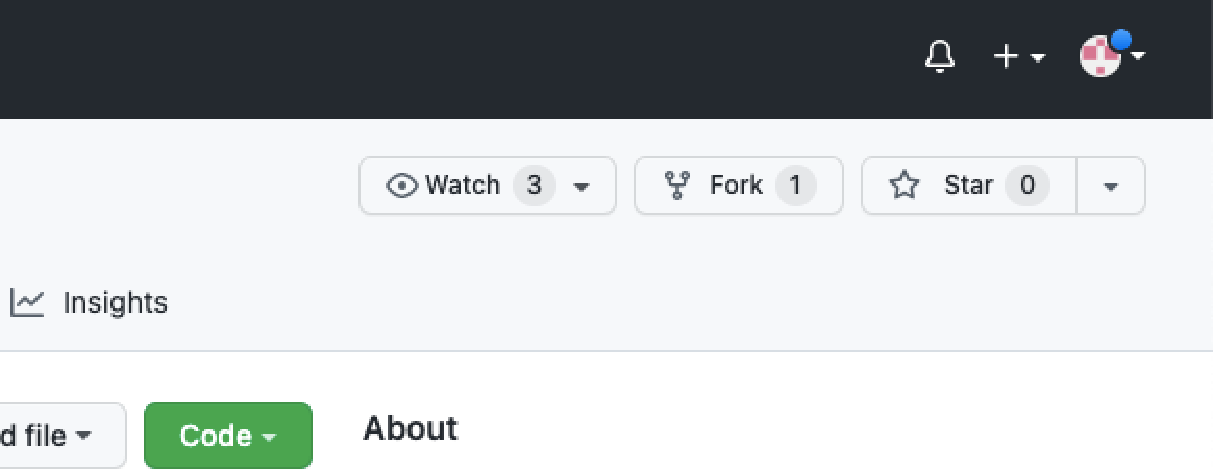
\includegraphics[width=\linewidth]{external/hub_fork.pdf}
\end{image}%
\tcblower
\end{figureptx}%
\begin{activity}{Activity}{Forking On GitHub.}{activity-act-hub-fork}%
This activity focuses on forking a repo and getting a new project started that we will carry throughout this chapter: editing a file on a repository I created.%
\begin{enumerate}[font=\bfseries,label=(\alph*),ref=\alph*]%
\item{}First, navigate to my \href{https://github.com/ian-curtis/aboutme}{\mono{aboutme} repository on GitHub}\footnotemark{}.%
\item{}Locate the ``Fork'' button in the top right corner.%
\par
Note the number next to it. This indicates the number of people who have forked a repo. This also applies to the Watch (people who receive notifications for the repo) and Star buttons. A good sense of how popular and how useful the contents of the repo are can be gained from looking at these numbers (where higher is better.)%
\item{}Click on the Fork button. A new webpage will appear allowing you to rename your fork and add a description. I recommend keeping the same name as the parent repository, as GitHub suggests. This will make it easier to remember what the repo is for.%
\par
That being said, you cannot have two repos with the same name. If you have been following along with the book, you might already have a repository named \mono{aboutme}. In that case, you should choose a different name, but one that is close or similar to the parent repo's.%
\par
Click on the Create Fork button.%
\item{}After a few seconds, your own fork will appear! Take a look at the top left corner where the name of the repo is displayed. You should notice that your personal username and repo name are there. But underneath that, in smaller font, GitHub tells you the username and repo name from which you forked. This is useful for reminding yourself that you are working on a copy of a repository, not the authoritative one.%
\end{enumerate}%
\end{activity}%
\footnotetext[52]{\nolinkurl{github.com/ian-curtis/aboutme}\label{fn-act-hub-fork-c-a-a-b}}%
Congrats! You've just forked a repository! If you plan on collaborating with others forking will become something you get very used to.%
\par
Remember that you just created a copy of my repository. You can make all the changes you want on your copy without asking for permisson from me. But as soon as you try to update my repo, you will have to submit a pull request. A fork is where you edit some things, try some things, and break some things before making a final product of whatever it is you were working on. Then send the changes over to the main repo!%
\end{subsectionptx}
\end{sectionptx}
%
%
\typeout{************************************************}
\typeout{Section 5.3 Editing}
\typeout{************************************************}
%
\begin{sectionptx}{Section}{Editing}{}{Editing}{}{}{section-S_hubcollabedit}
\index{github!collaborate}%
\index{markdown}%
This part should seem familiar. Remember how to edit files on GitHub? (Hint: \hyperref[subsection-hub-editfile]{Subsection~{\xreffont\ref{subsection-hub-editfile}}}.) Let's try editing a file on my \mono{aboutme} repo. Click on the \mono{aboutyou.md} file on the home page of the repo. This is a Markdown file, just like the README we were working with in \hyperref[section-S_hubfirstrepo]{Section~{\xreffont\ref{section-S_hubfirstrepo}}}. Follow \hyperref[activity-edit-aboutyou]{Activity~{\xreffont\ref{activity-edit-aboutyou}}} to edit this file. Remember, things should look very similar to \hyperref[assemblage-markdown]{Markdown Basics} and \hyperref[exercise-try-markdown]{Checkpoint~{\xreffont\ref{exercise-try-markdown}}}.%
\begin{activity}{Activity}{Collaboration Editing: Start With Yourself.}{activity-edit-aboutyou}%
When most people collaborate, they make a bunch of changes on their fork. Then, when the changes are ready, they send them over to the main repository. This activity focuses on the first part of that process, editing files on your own fork.%
\begin{enumerate}[font=\bfseries,label=(\alph*),ref=\alph*]%
\item{}Click on the ``edit'' button (the pencil icon on the right side of the page)%
\item{}Follow the instructions on the file to add your own entry.%
\begin{quote}%
To contribute, add your name as a level two heading. This can be just your first name, just your last name, both, all names, initials, a name you like, your GitHub username, etc. In a paragraph, type the month, year, and the country and\slash{}or state\slash{}province you are contributing from. If you feel like it, tell us something cool about you! (See my example.)%
\par
Responses will be moderated. No explicit content whatsoever will be accepted (keep things G rated please!).%
\end{quote}
\item{}Once you are done editing, head to the Commit changes dialog. In the box that is autofilled with ``Update aboutyou.md'', type a more informative commit message. A description is not necessary.%
\item{}Do not select the button that says ``Commit directly to the \mono{main} branch''. It is always a good idea to create a branch when editing someone else's work.%
\par
Select the button that allows you to create a new branch and type in a better branch name.%
\item{}Notice that the button now says ``propose changes'' rather than ``commit changes''. Again, this is because you do not have permission to commit changes to my repo, just propose them. Click on this button once you have changed the branch name.%
\item{}This will conveniently bring you right to the pull request page, which might look familiar. Your previous commit message will automatically be there. The only thing you really need to do is click on ``Create pull request''. (But read below before you click it.)%
\par
Also take note at the top of this page GitHub tells you what branches are being merged. You will probably see%
\begin{quote}%
\mono{base: main} \faArrowLeft{} \mono{compare: <your-branch-name>}.%
\end{quote}
If not, use the dropdown menus to make yours look like the above. This means that you are taking your branch and attempting to merge your changes into the main branch from the ``base'' repository, or \emph{your repo}.%
\par
Like before, if you scroll down, you can see all of the changes you made. Later, I will be able to see this too, to make sure that you only changed what you were supposed to and didn't write anything R-rated.%
\par
Now you can create the pull request.%
\item{}Here, you are asking yourself for permission to merge into your fork. Hopefully you give yourself permission to do so. Click on ``Merge pull request'' and then ``Confirm merge''. You may delete the branch if you'd like.%
\end{enumerate}%
\end{activity}%
Assuming you have completed \hyperref[activity-edit-aboutyou]{Activity~{\xreffont\ref{activity-edit-aboutyou}}}, you might notice that a new box has popped up in the main page of your fork. It might say something like ``This branch is 2 commits ahead of \mono{ian-curtis:main}''. This is how you create a pull request.%
\par
Now you can make as many changes and commits as you want before opening a pull request (this will change the message on the dialog box). You don't even have to merge your changes into your fork's main branch before opening a pull request. However, I usually choose to do so just so I know that all of my changes from my various branches are included where they are supposed to be. Feel free to continue making edits and\slash{}or commits to your entry in the \mono{aboutyou.md} file before continuing!%
\begin{activity}{Activity}{Collaboration Editing: Sending Your Changes Away.}{activity-collab-pr}%
\index{pull request}%
\index{github!pull request}%
\index{base repository}%
\index{head repository}%
\index{merge}%
\index{github!merge}%
This activity assumes you have been following along throughout the section. \hyperref[activity-edit-aboutyou]{Activity~{\xreffont\ref{activity-edit-aboutyou}}} must be completed before this activity. Just like in \hyperref[subsection-SS_pullrequest]{Subsection~{\xreffont\ref{subsection-SS_pullrequest}}}, we will use the ``Contribute'' option on the Code tab of a repo (see \hyperref[figure-fig-hubcollab-contrib]{Figure~{\xreffont\ref{figure-fig-hubcollab-contrib}}}) even though there are other ways to open a pull request.%
\begin{figureptx}{Figure}{The Contribute dialog box on GitHub.}{figure-fig-hubcollab-contrib}{}%
\begin{image}{0.025}{0.95}{0.025}{}%
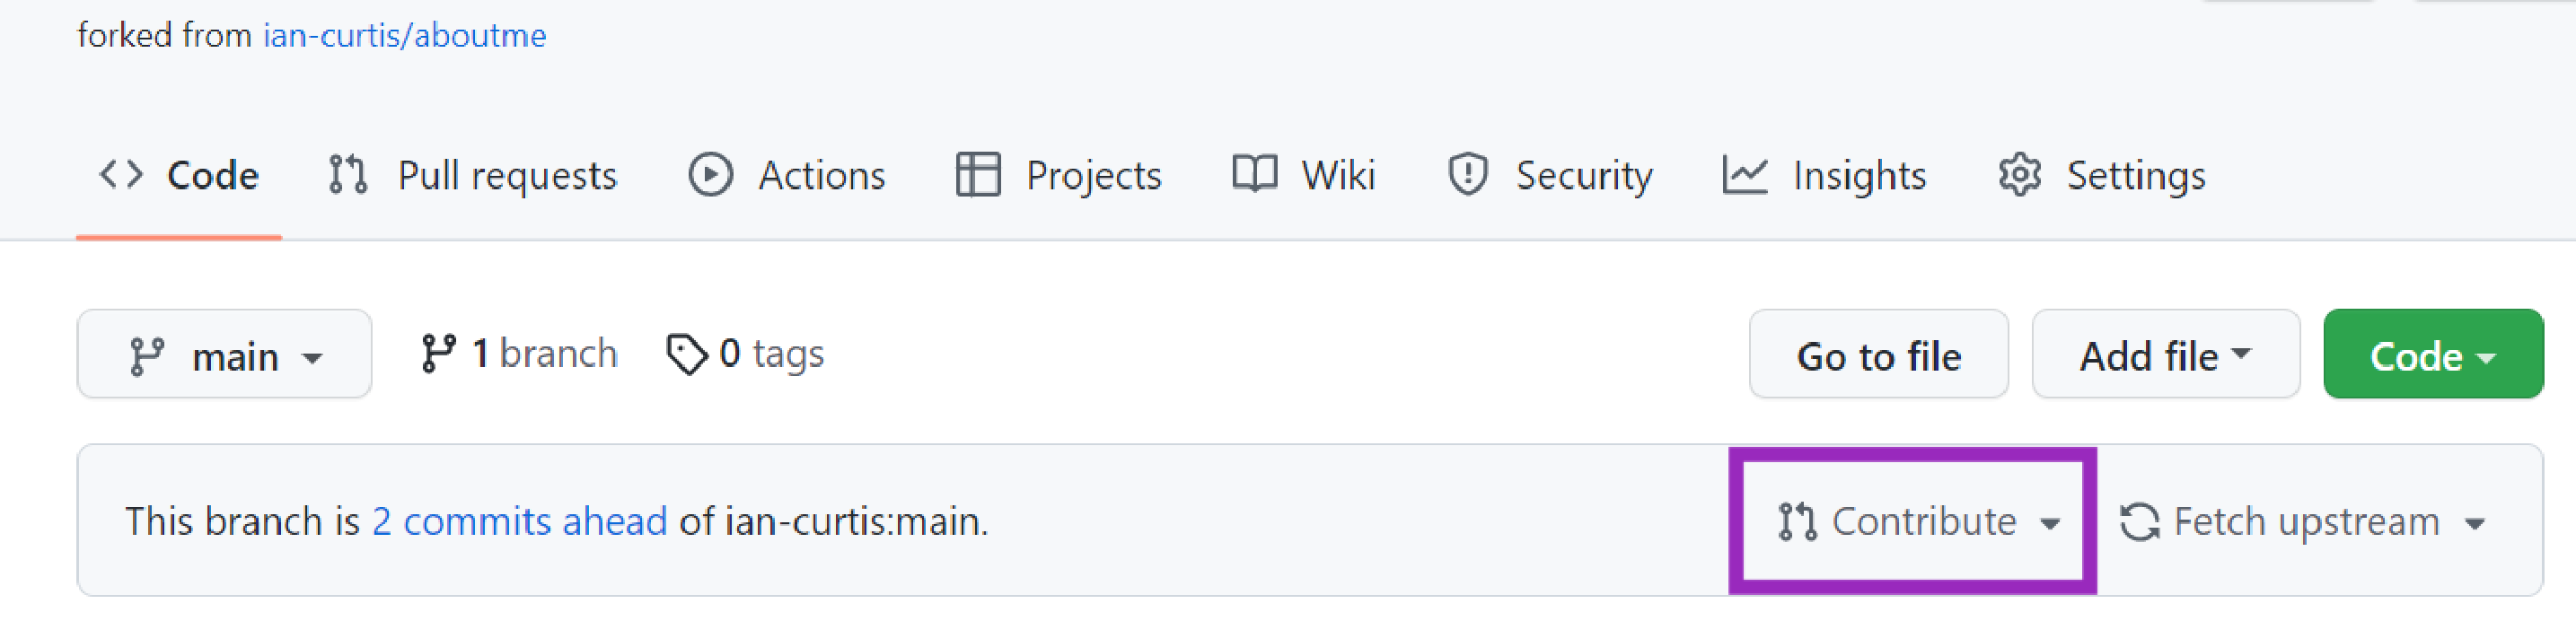
\includegraphics[width=\linewidth]{external/hubcollab_contrib.pdf}
\end{image}%
\tcblower
\end{figureptx}%
\begin{enumerate}[font=\bfseries,label=(\alph*),ref=\alph*]%
\item{}Make sure you are on your fork's home page (the Code tab). Click on the Contribute drop down menu and then the ``Open pull request'' button. This will bring you to a new page containing familiar elements.%
\item{}This task is all about noticing. Take a minute to identify each of the following elements on the page. These will help you in the future to recognize that you are opening a pull request for someone else's repository and can be a reassurance that you are in the right place.%
\begin{enumerate}
\item{}The title of the repository has changed. You are no longer on your fork, but on the forked-from repo. As such, the Watch, Fork, and Star data have changed to describe that authoritative repo.%
\item{}There is a dialog box indicating which branches are being merged. There are more boxes than before. There should be four, allowing you to specify which repo and branch to want to merge from and which repo and branch you want to merge to. Usually GitHub gets it right, but not always, so check to make sure these are what you want.%
\par
The \terminology{base repository} is the repo you are merging to (here, the authoritative repo), the \terminology{head repository} is the repo you are merging from (here, your fork). The base branch is the specific branch you are merging to (often \mono{main}) and the compare branch is the branch from your fork you are merging from (often \mono{main} for me personally).%
\item{}After these boxes is, hopefully, a green checkmark and an ``Able to merge'' message. This is what you want. You might also get a red message about conflicts or other messages. In this case, you might have a merge conflict and will need to do some extra work. See \hyperref[section-S_mergeconflict]{Section~{\xreffont\ref{section-S_mergeconflict}}}.%
\item{}There is a summary of all the commits made on the branch (with their commit messages)%
\item{}There is info on all of your specific changes in each file%
\end{enumerate}
%
\item{}Once you have found all of the above, go ahead and click on the ``Create pull request'' button. If your pull request has more than one commit, you will have to enter a title for the request. This is where a description might be helpful. Choose a title that describes what you are doing. If you would like to supply more information, ask a question, or give clarification, type as much as you want into the ``Leave a comment'' text box. Then click ``Create pull request''.%
\item{}This time notice that there is no option to ``Merge'' into the main branch. This is because you do not have write access to the parent repository. At this point, wait for a moderator from the authoritative repo to approve your pull request.%
\end{enumerate}%
\end{activity}%
Note that forking can drastically increase the complexity of the GitHub tree. Recall from \hyperref[figure-fig-hub-animal-merge]{Figure~{\xreffont\ref{figure-fig-hub-animal-merge}}} that branches make another branch on the tree which you eventually merge back into the main branch, or the trunk of the tree. Cloning made this more complex due to the copy on your computer. Forking adds another copy into the mix. \hyperref[figure-fig-collab-fork]{Figure~{\xreffont\ref{figure-fig-collab-fork}}} provides a possible diagram of the forking process. But there are many different variations to this diagram as it is up to you how many branches\slash{}commits to make and to which branch you push.%
\begin{figureptx}{Figure}{Example of GitHub Tree with a fork}{figure-fig-collab-fork}{}%
\begin{image}{0.025}{0.95}{0.025}{}%
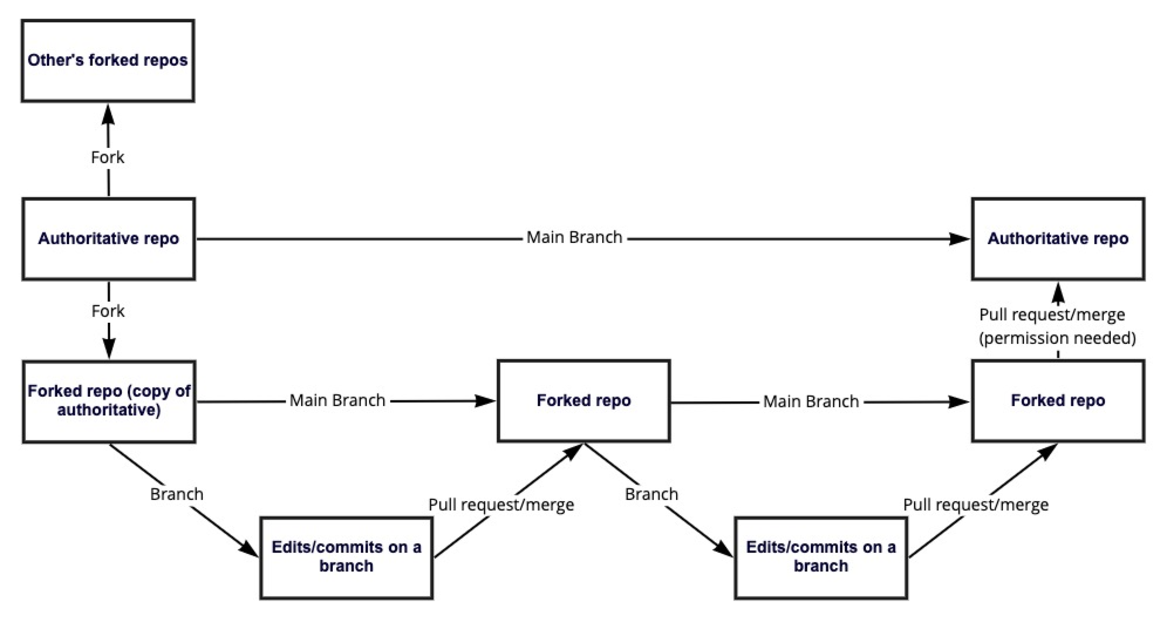
\includegraphics[width=\linewidth]{external/collab_fork.pdf}
\end{image}%
\tcblower
\end{figureptx}%
Now you can sit back and relax until a moderator reviews your contribution. If they make a comment or approve your pull request, you will get an email to the email address on your account. Once they approve your work, great! Congrats! Are you done? Proceed to \hyperref[section-S_hubcollabfetch]{Section~{\xreffont\ref{section-S_hubcollabfetch}}} to find out!%
\end{sectionptx}
%
%
\typeout{************************************************}
\typeout{Section 5.4 Fetching Upstream}
\typeout{************************************************}
%
\begin{sectionptx}{Section}{Fetching Upstream}{}{Fetching Upstream}{}{}{section-S_hubcollabfetch}
%
%
\typeout{************************************************}
\typeout{Subsection 5.4.1 First, Fetching}
\typeout{************************************************}
%
\begin{subsectionptx}{Subsection}{First, Fetching}{}{First, Fetching}{}{}{subsection-SS_fetch}
\index{fetch}%
\index{github!fetch}%
To answer the question in \hyperref[section-S_hubcollabedit]{Section~{\xreffont\ref{section-S_hubcollabedit}}}, we are not quite done. See, even though your fork and the parent repository are connected, updates in one are not automatically reflected in the other. So if you just contributed to a repository and the pull request was accepted, you should be fine. But if someone else's pull request also got approved, your fork will not have those changes. You have to tell GitHub to grab those changes and update your fork.%
\par
The act of grabbing changes from the parent repository is called \terminology{fetching}, aptly named since that is exactly what you are doing: fetching changes. Technically, this is distinct from a related \terminology{merge}. First, you fetch the changes, then you merge the changes into your fork.%
\par
You might remember from previous sections using \mono{git pull} to fetch changes. In essence, using this command will fetch your changes. But it also merges the changes into your fork. In most cases, using \mono{git pull} is fine and is a great shortcut. But as you get more experienced in the git world, you may want to fetch changes and then merge them later. We will explore pulling changes more in future sections.%
\par
Before continuing, you must wait until I accept your pull request from \hyperref[section-S_hubcollabedit]{Section~{\xreffont\ref{section-S_hubcollabedit}}}.%
\end{subsectionptx}
%
%
\typeout{************************************************}
\typeout{Subsection 5.4.2 Second, Upstream}
\typeout{************************************************}
%
\begin{subsectionptx}{Subsection}{Second, Upstream}{}{Second, Upstream}{}{}{subsection-SS_upstream}
\index{upstream}%
\index{remote!upstream}%
Another important concept is that of \terminology{upstream}. Remember from \hyperref[subsection-SS_git-push]{Subsection~{\xreffont\ref{subsection-SS_git-push}}} when we talked about remotes? Back there, I mentioned that there were two types of remotes (origin and upstream) and that we would talk about upstream later. Well, now it's later! This idea will become important again when we use Git to collaborate (see if you can figure out why).%
\par
Any repository you own or that you clone will have the remote identifier of ``origin'', for you. Any repo you do not own \emph{and that you fork} will have the remote identifier of ``upstream''. Remember that a remote is like a connection between repositories; it's the definition of the link between them. When you fork a repo, you are creating a remote connection between the parent repo (upstream) and your newly-created fork (origin). As we will explore in \hyperref[chapter-C_gitcollab]{Chapter~{\xreffont\ref{chapter-C_gitcollab}}}, when you clone a repo, you are creating a remote connection between your fork (origin) and your personal computer (local) with the future ability to be connected to the authoritative repo (upstream).%
\end{subsectionptx}
%
%
\typeout{************************************************}
\typeout{Subsection 5.4.3 Third, Fetching Upstream}
\typeout{************************************************}
%
\begin{subsectionptx}{Subsection}{Third, Fetching Upstream}{}{Third, Fetching Upstream}{}{}{subsection-SS_fetchupstream}
\index{fetch upstream}%
\index{github!fetch}%
So in order to have changes from the parent repository reflected in your own fork, you have to \terminology{fetch upstream}. GitHub makes this easy! Remember that dialog box from \hyperref[activity-collab-pr]{Activity~{\xreffont\ref{activity-collab-pr}}}? Back then, we used the ``Contribute'' button to start a pull request. Here, we will use the option right next to it: ``Fetch upstream''.%
\par
First, though, go back to the homepage of your fork. You might notice that a slightly different box has appeared. Now it might say something like ``This branch is 1 commit \emph{behind} \mono{ian-curtis:main}'' (you could have a different number). Earlier you were \emph{ahead} of \mono{ian-curtis:main}. What's going on here?%
\begin{assemblage}{Assemblage}{Ahead vs. Behind.}{assemblage-ahead-behind}%
GitHub uses \terminology{ahead} and \terminology{behind} to tell you how your fork currently sits compared to the repo you forked from. Any commit that you have made to your fork that has not been merged into the parent repo ticks up the number of commits ahead you are. Any commit that has been made to the parent repo that is not reflected in your fork ticks up the number of commits behind you are.%
\par
As an example, you might have a message like ``This branch is 2 commits ahead, 3 commits behind \mono{<parent-repo>:main}''. This means you have made 2 commits that are not on the parent repo and that the parent repo has 3 commits that you have not fetched.%
\end{assemblage}
\begin{warning}{Warning}{Fetch Upstream Often.}{warning-warn-fetch-often}%
In my opinion, you want to keep the least amount of commits behind. If you are working on someone else's work, you want to stay up to date. If some big change happens, you should make sure you have that change on your fork. Why? Well, you don't want to overwrite anything someone else just did. You also don't want to work on adding a new feature that is already incorporated. Maybe the new change helps you do your work better\slash{}faster. You also want to avoid potential merge conflicts because someone else changed the same files you are working on.%
\par
Therefore, it is usually recommended practice to fetch upstream as often as you can. At the very least, daily, especially if the project is popular and updated frequently. It is possible that there is no new upstream content to fetch but hey, at least you checked!%
\par
This warning will repeat in \hyperref[chapter-C_gitcollab]{Chapter~{\xreffont\ref{chapter-C_gitcollab}}} when we talk about pulling and pushing.%
\end{warning}
You may be wondering why you are even any commits behind! If your addition to my repository was accepted, then our repos should match, right? Not quite. Actually, that act of accepting your pull request and merging into my main branch was a commit in itself which is where the mystery commit comes from.%
\begin{activity}{Activity}{Fetching Upstream.}{activity-act-fetch-upstream}%
Enough talk, let's fetch that upstream!%
\begin{enumerate}[font=\bfseries,label=(\alph*),ref=\alph*]%
\item{}Find the ``Fetch upstream'' dialog box on the home page of your fork.%
\item{}Notice that GitHub will fetch and merge the upstream changes in one step (even though it is technically two steps). Great!%
\par
It also emphasizes \hyperref[warning-warn-fetch-often]{Warning~{\xreffont\ref{warning-warn-fetch-often}}} through a somewhat passive-aggressive reminder: ``Keep your fork up-to-date with the upstream repository''.%
\par
To make the magic happen, click on ``Fetch and merge''.%
\item{}Bam. Done. But do make sure your fork now says%
\begin{quote}%
This branch is up to date with \mono{ian-curtis/aboutme:main}%
\end{quote}
(in general, this would be the name of whatever repo you forked from). Yours may also say, depending on when you fetched, that your branch is a number of commits ahead (but none behind).%
\end{enumerate}%
\end{activity}%
\end{subsectionptx}
\begin{conclusion}{}%
And there you go! Now you are ready to keep on editing or to go about your day. If you are interested in some other GitHub features related to collaborating, continue to \hyperref[appendix-app_hubextra]{Appendix~{\xreffont\ref{appendix-app_hubextra}}}. Otherwise, go to \hyperref[chapter-C_gitcollab]{Chapter~{\xreffont\ref{chapter-C_gitcollab}}} to see how to use Git commands and local edits to collaborate.%
\end{conclusion}%
\end{sectionptx}
\end{chapterptx}
 %
%
\typeout{************************************************}
\typeout{Chapter 6 Git Collaboration}
\typeout{************************************************}
%
\begin{chapterptx}{Chapter}{Git Collaboration}{}{Git Collaboration}{}{}{chapter-C_gitcollab}
\renewcommand*{\chaptername}{Chapter}
\begin{introduction}{}%
This chapter is closely related to \hyperref[chapter-C_gitsolo]{Chapter~{\xreffont\ref{chapter-C_gitsolo}}} and \hyperref[chapter-C_githubcollab]{Chapter~{\xreffont\ref{chapter-C_githubcollab}}} in that the concepts there carry over and are combined together here. The workflow and steps described in this chapter are most similar to the typical day-to-day work from many people around the world when it comes to Git and GitHub.%
\end{introduction}%
%
%
\typeout{************************************************}
\typeout{Section 6.1 Getting Set Up: A Few Extra Steps}
\typeout{************************************************}
%
\begin{sectionptx}{Section}{Getting Set Up: A Few Extra Steps}{}{Getting Set Up: A Few Extra Steps}{}{}{section-S_gitcollabsetup}
\index{fork}%
\begin{introduction}{}%
Before you are able to jump right in and start editing files locally, there are some things that have to happen first. Like in \hyperref[section-S_hubcollabsetup]{Section~{\xreffont\ref{section-S_hubcollabsetup}}}, we need to fork the repository you would like to edit. Although it is possible to use Git to edit on a repository that has not been forked, you will find problems when you try to push your changes since you do not have write access to the repo.%
\par
So, to continue on with this section, make sure you have my \mono{aboutme} repository forked. Recall that we did this in \hyperref[subsection-SS_forking]{Subsection~{\xreffont\ref{subsection-SS_forking}}}. If you've done this already, you do not need to do it again. If you haven't, review the instructions in \hyperref[subsection-SS_forking]{Subsection~{\xreffont\ref{subsection-SS_forking}}}.%
\par
I would also like to repeat something I said back in \hyperref[section-S_gitsetup]{Section~{\xreffont\ref{section-S_gitsetup}}}:%
\begin{quote}%
It's not always feasible to edit file on GitHub, as we did in \hyperref[section-S_hubfirstrepo]{Section~{\xreffont\ref{section-S_hubfirstrepo}}} and \hyperref[section-S_hubbranches]{Section~{\xreffont\ref{section-S_hubbranches}}}. Certain text editors (for instance, Visual Studio Code which you might also have installed) have features built in to ease coding and file editing. \initialism{VS} Code extensions might add color to text to help you see what's going on in your code. Others provide bug fixing and error catching before the errors actually occur. In general, you will edit files on your personal computer and will want to share them with the world. \emph{I would stay away from editing on GitHub unless you have a small correction and\slash{}or you don't need any special editing tools.}%
\end{quote}
The rest of this section and chapter will look a lot like \hyperref[section-S_gitsetup]{Section~{\xreffont\ref{section-S_gitsetup}}} and \hyperref[chapter-C_gitsolo]{Chapter~{\xreffont\ref{chapter-C_gitsolo}}} with a few changes. With that being said, do you remember what the first step to editing locally was?%
\end{introduction}%
%
%
\typeout{************************************************}
\typeout{Subsection 6.1.1 Cloning A Fork}
\typeout{************************************************}
%
\begin{subsectionptx}{Subsection}{Cloning A Fork}{}{Cloning A Fork}{}{}{subsection-SS_gitcollabclone}
\index{clone}%
\index{git!clone}%
Hopefully you didn't peek ahead! The first step is to clone our repo. Remember that in order to edit files locally, we need a copy of the repository on our computer and the way to do that is to clone.%
\par
This again increases the complexity of the Git tree. From an authoritative repo we made a copy on GitHub, called a fork. We did this so that we could have all freedom to edit the files as we pleased without breaking any of the official files. From there, we need to clone to make a copy of the fork on our computer. Do make sure you are cloning your fork, \emph{not the repo you forked}.%
\begin{inlineexercise}{Checkpoint}{}{exercise-SS_gitcollabclone-f}%
So go ahead, use your terminal clone your fork of my \mono{aboutme} repository. Before you do so, make sure that your branch is up to date with \mono{ian-curtis/aboutme:main}.%
\par
Don't remember how to do this? \hyperref[project-try-git-clone]{Git Procedure~{\xreffont\ref{project-try-git-clone}}} might be useful, as may be the solution to this exercise.%
\end{inlineexercise}%
Great! Your repo should now be cloned on to your computer. Carry on.%
\end{subsectionptx}
%
%
\typeout{************************************************}
\typeout{Subsection 6.1.2 Don't Forget About Branches!}
\typeout{************************************************}
%
\begin{subsectionptx}{Subsection}{Don't Forget About Branches!}{}{Don't Forget About Branches!}{}{}{subsection-SS_gitcollabbranch}
\index{branches}%
\index{git!branches}%
For nearly every edit we've made in this book, we've made a corresponding branch. This is no different. I hope you understand the importance of branches, even if you are working with yourself.%
\par
Since my repository is public, anyone can edit the files there. Therefore, I will approve pull requests from anyone as I will assume they are working through this book. However, the task in this chapter will be exclusive to just those who are reading this book. There is file called \mono{secret.txt} with no instructions or anything at all. Later on, you will be adding a line to this text file.%
\par
For now, create a good branch name for this edit, perhaps \mono{secret}? Remember that cloning a repo does not navigate inside of the repo so make sure you use \mono{cd <your-repo-name>} before creating a branch.%
\begin{inlineexercise}{Checkpoint}{}{exercise-SS_gitcollabbranch-g}%
Make a new branch. Switch to that branch. See \hyperref[subsection-SS_gitbranches]{Subsection~{\xreffont\ref{subsection-SS_gitbranches}}} if you need a refresher.%
\end{inlineexercise}%
\begin{figureptx}{Figure}{Diagram of a fork, a clone, and a branch}{figure-fig-git-fork-clone}{}%
\begin{image}{0.1}{0.8}{0.1}{}%
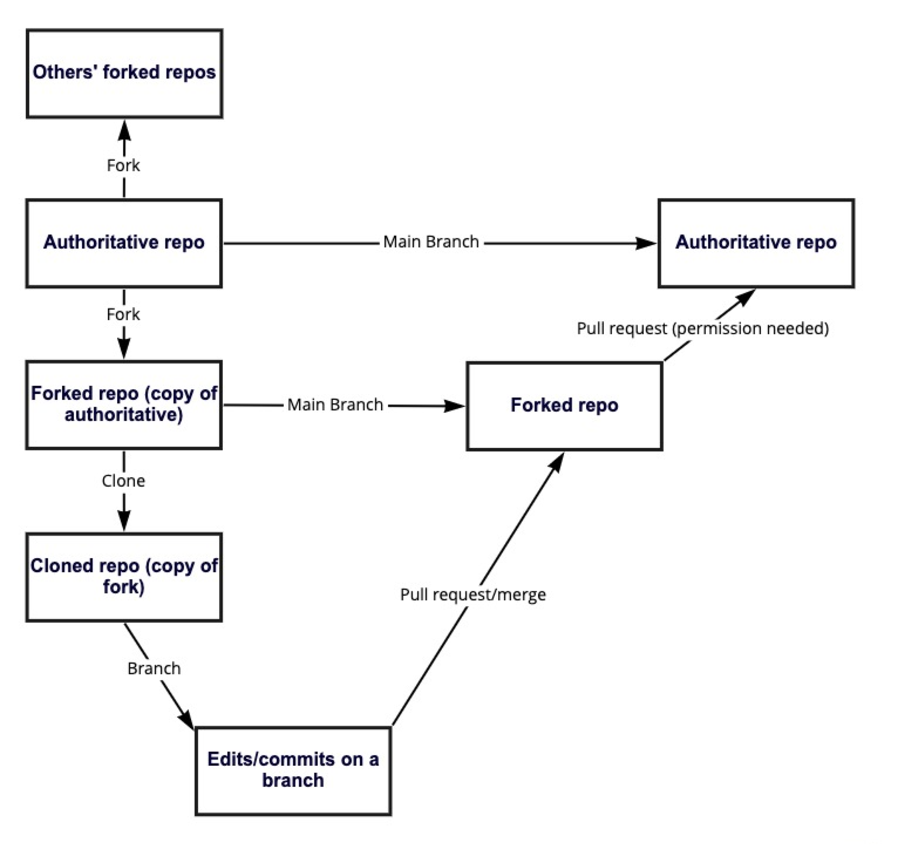
\includegraphics[width=\linewidth]{external/git_fork_clone.pdf}
\end{image}%
\tcblower
\end{figureptx}%
Take a look at \hyperref[figure-fig-git-fork-clone]{Figure~{\xreffont\ref{figure-fig-git-fork-clone}}} for a visualization of what the Git tree might look like at the end of the editing process. This is the end goal. Then, let's get to editing.%
\end{subsectionptx}
\end{sectionptx}
%
%
\typeout{************************************************}
\typeout{Section 6.2 Collaboration Editing With Git}
\typeout{************************************************}
%
\begin{sectionptx}{Section}{Collaboration Editing With Git}{}{Collaboration Editing With Git}{}{}{section-S_gitcollabedit}
\index{edit files}%
\index{git!edit}%
As before, the title is a little misleading. Git does not offer editing features, but, once again, it does keep track of your edits and commits for version control.%
\par
This section will be very short. All you need to do is open \mono{secret.txt} and type one line of whatever you want (G-rated of course). Literally could be anything. Just something random. Maybe the following will inspire you:%
\begin{itemize}[label=\textbullet]
\item{}``Tick tock'' went the tick tock croc.%
\item{}Have you ever tried ham and peanut butter?%
\item{}The jalapeño, who was too hot, walked into the ocean to cool off and was eaten by a shark who became the first creature to breath fire underwater.%
\item{}I recently tripped up the stairs.%
\end{itemize}
%
\par
Whatever you choose, try to stick to one or two lines. When you are done, save the file (which will tell Git that there are active changes) and move on. The next steps are similar, but not exactly the same as those in \hyperref[section-S_gitfinalize]{Section~{\xreffont\ref{section-S_gitfinalize}}}.%
\end{sectionptx}
%
%
\typeout{************************************************}
\typeout{Section 6.3 Revisiting the Three Step Process}
\typeout{************************************************}
%
\begin{sectionptx}{Section}{Revisiting the Three Step Process}{}{Revisiting the Three Step Process}{}{}{section-S_gitcollabfinalize}
\index{three step process}%
\index{git!three step process}%
\begin{introduction}{}%
Just as in \hyperref[section-S_gitfinalize]{Section~{\xreffont\ref{section-S_gitfinalize}}}, this is a very important section. Take care to do everything in the correct order and with the correct keywords.%
\par
Recall that the three step process for sending changes back to GitHub consists of%
\begin{enumerate}
\item{}Staging your files for sending%
\item{}Commiting your changes%
\item{}Pushing your changes to GitHub%
\end{enumerate}
%
\par
Since we've already covered much of this material, I won't go into as much detail. I will, however, point out any significant differences. As you move forward, don't forget about the handy \mono{git status} command to remind you what files have been edited, staged, or committed.%
\end{introduction}%
%
%
\typeout{************************************************}
\typeout{Subsection 6.3.1 Staging Files}
\typeout{************************************************}
%
\begin{subsectionptx}{Subsection}{Staging Files}{}{Staging Files}{}{}{subsection-SS_gitcollabadd}
\index{staging}%
\index{git!stage}%
This step will not be any different from before. Use \hyperref[project-try-git-add]{Git Procedure~{\xreffont\ref{project-try-git-add}}} to stage your edited \mono{secret.txt} file.%
\par
Remember that \mono{git add} is pretty flexible. If you've edited more than one file, you can choose which files to add. Maybe you want to make two commits. In that case, stage some files and commit them, then stage the other files and commit them.%
\end{subsectionptx}
%
%
\typeout{************************************************}
\typeout{Subsection 6.3.2 Committing Files}
\typeout{************************************************}
%
\begin{subsectionptx}{Subsection}{Committing Files}{}{Committing Files}{}{}{subsection-SS_gitcollabcommit}
\index{commit files}%
\index{git!commit}%
This step will also not be any different from before. Just remember that you should try to design your commit messages to be short and descriptive. If the repo you are contributing to has a preference for how commit messages are written, you should try to follow that as best you can. Otherwise, don't be offended when your commit message is changed.%
\par
\hyperref[project-try-git-commit]{Git Procedure~{\xreffont\ref{project-try-git-commit}}} will probably be helpful as will the reminders at the end of \hyperref[subsection-SS_git-commit]{Subsection~{\xreffont\ref{subsection-SS_git-commit}}}. Commit your \mono{secret.txt} file and provide an apt commit message (especially one that shows you were reading this book).%
\end{subsectionptx}
%
%
\typeout{************************************************}
\typeout{Subsection 6.3.3 Pushing Files}
\typeout{************************************************}
%
\begin{subsectionptx}{Subsection}{Pushing Files}{}{Pushing Files}{}{}{subsection-SS_gitcollabpush}
\index{push files}%
\index{git!push}%
Alright, here is where some small changes come up. In \hyperref[section-S_gitfinalize]{Section~{\xreffont\ref{section-S_gitfinalize}}}, we pushed to the origin repository. But from \hyperref[section-S_hubcollabsetup]{Section~{\xreffont\ref{section-S_hubcollabsetup}}} and \hyperref[section-S_hubcollabfetch]{Section~{\xreffont\ref{section-S_hubcollabfetch}}}, when you fork, you introduce another remote: upstream. And now that we have a clone, we also have a local repo.%
\par
Alright, so what about right now? You have your changes staged and committed, but to where do you push? Local? That won't work since you already have the changes locally. Upstream? It might make sense to push directly to the authoritative repo, but since you don't have write access, this will likely not work. The right thing to do here is push to origin. Remember, ``origin'' in this case, refers to your fork.%
\par
From \hyperref[subsection-SS_git-push]{Subsection~{\xreffont\ref{subsection-SS_git-push}}} (and \hyperref[project-try-git-push]{Git Procedure~{\xreffont\ref{project-try-git-push}}}) can you figure out what to type into the terminal to push to origin?%
\par
Remember you need to specify the remote and the branch you are pushing to so \mono{git push origin <branch-name>} will do nicely.%
\end{subsectionptx}
\begin{conclusion}{}%
Believe it or not, \hyperref[project-three-step-summ]{Git Procedure~{\xreffont\ref{project-three-step-summ}}} was written in generic terms, so it applies here as well! Keep it handy, or perhaps keep \hyperref[section-S_gitsumm]{Section~{\xreffont\ref{section-S_gitsumm}}} and \hyperref[section-S_gitcollabsumm]{Section~{\xreffont\ref{section-S_gitcollabsumm}}} in mind as you proceed in your Git career. Now let's go create a pull request from that push we just made.%
\end{conclusion}%
\end{sectionptx}
%
%
\typeout{************************************************}
\typeout{Section 6.4 The Final Steps}
\typeout{************************************************}
%
\begin{sectionptx}{Section}{The Final Steps}{}{The Final Steps}{}{}{section-S_gitcollabpr}
\begin{introduction}{}%
All that's left to do is to create some pull requests. There are technically two ways you could make this work. You can either open a pull request from your new branch directly to the authoritative main branch or you can merge from your new branch to your fork's main branch and then to the authoritative main branch.%
\end{introduction}%
%
%
\typeout{************************************************}
\typeout{Subsection 6.4.1 Opening a Pull Request}
\typeout{************************************************}
%
\begin{subsectionptx}{Subsection}{Opening a Pull Request}{}{Opening a Pull Request}{}{}{subsection-SS_gitcollabpr}
\index{pull request}%
\index{github!pull request}%
\index{merge}%
\index{github!merge}%
\index{head repository}%
\index{base repository}%
Use \hyperref[activity-act-git-pr]{Activity~{\xreffont\ref{activity-act-git-pr}}} to go back to GitHub and start opening a pull request. When you arrive at the pull request creation screen (titled ``Comparing changes''), you generally have two choices, as mentioned above. The following list describes the branches and repos you should have selected at the top of the screen, under the page heading.%
\begin{enumerate}
\item{}\lititle{Merge from your new branch to your fork, then to the authoritative.}\par%
Your base repository should be \mono{<your-username>/<your-fork>}, base should be \mono{main}, and compare should be \mono{<your-branch}. Do note that once you select your fork for the base repository, the page will reload and the base and head repository options will disappear.%
\par
Then, click Create pull request and merge in to main. You may now open another pull request with options base repository of \mono{<authoritative-username>/<authoritative-repo>}, base should be \mono{main}, head repository should be \mono{<your-username><your-fork>} and compare should be \mono{main}.%
\item{}\lititle{Merge from your new branch directly to the authoritative.}\par%
Your base repository should be \mono{<authoritative-username>/<authoritative-repo>}, base should be \mono{main}, head repository should be \mono{<your-username><your-fork>} and compare should be \mono{<your-branch>}.%
\end{enumerate}
%
\par
After either of those two, click on ``Create pull request'', enter a title, and click ``Create pull request'' again. From there, you will have to wait for approval and moderator merge.%
\end{subsectionptx}
%
%
\typeout{************************************************}
\typeout{Subsection 6.4.2 Pulling\slash{}Fetching Upstream}
\typeout{************************************************}
%
\begin{subsectionptx}{Subsection}{Pulling\slash{}Fetching Upstream}{}{Pulling\slash{}Fetching Upstream}{}{}{subsection-SS_gitcollabpull}
\index{fetch upstream}%
\index{upstream}%
\index{remote!upstream}%
\index{pull}%
\index{git!pull}%
Recall from \hyperref[section-S_hubcollabfetch]{Section~{\xreffont\ref{section-S_hubcollabfetch}}} that you can update your fork with the latest upstream changes through the ``Fetch upstream'' button. That works great for updating the fork, but it doesn't update your local clone. There are two main ways in which you can update both your fork and your clone with new changes to upstream.%
\begin{project}{Git Procedure}{Updating Origin and Local, Method 1.}{project-try-git-pull-origin}%
\index{git!pull}%
\index{pull}%
\index{origin}%
\index{remote!origin}%
This method will first fetch upstream on GitHub, then pull in changes from origin.%
\begin{enumerate}[font=\bfseries,label=(\alph*),ref=\alph*]%
\item{}Use \hyperref[subsection-SS_fetchupstream]{Subsection~{\xreffont\ref{subsection-SS_fetchupstream}}} to fetch (and merge) upstream content into the main branch of your fork (origin).%
\item{}Now, head back to your terminal and make sure you are navigated to your clone. Do a check to make sure you are on your main branch; if not, use \mono{git switch main}.%
\par
If you are planning on making more changes to a branch, but want it updated to the latest upstream changes, you can stay on a branch. If you have any uncommitted changes, you might make a merge conflict.%
\item{}Now use \mono{git pull} to pull in the changes from your recently-updated fork. \hyperref[project-try-git-pull]{Git Procedure~{\xreffont\ref{project-try-git-pull}}} may be helpful. Just remember that you are pulling in changes from the main branch on origin.%
\end{enumerate}%
\end{project}%
\begin{project}{Git Procedure}{Updating Origin and Local, Method 2.}{project-try-git-pull-upstream}%
\index{git!add remote}%
\index{remote!origin}%
\index{remote!upstream}%
\index{upstream}%
\index{pull}%
\index{push}%
\index{git!pull}%
\index{git!push}%
This method will first set up a remote to upstream, pull in changes from upstream, then push changes to origin.%
\begin{enumerate}[font=\bfseries,label=(\alph*),ref=\alph*]%
\item{}Head to your terminal and make sure you are navigated to your clone. Do a check to make sure you are on your main branch; if not, use \mono{git switch main}.%
\par
If you are planning on making more changes to a branch, but want it updated to the latest upstream changes, you can stay on a branch. If you have any uncommitted changes, you might make a merge conflict.%
\item{}This step will only have to be done once per repo that you have forked, then cloned. When you clone a fork, the connection between origin and upstream is not carried over. If I tried to pull from upstream without this connection, I would get an error:%
\begin{console}{0}{1}{0}
> (*\consoleinput{git pull upstream main}*)
fatal: 'upstream' does not appear to be a git repository
fatal: Coult not read from remote repository.

Please make sure you have the correct access rights
and the repository exists.
\end{console}
This is troublesome! Clearly upstream exists; how else would we have forked it? To fix this, you need to manually set the remote connection. Again, this only has to be done once per forked\slash{}cloned repo.%
\begin{enumerate}[font=\bfseries,label=(\roman*),ref=\theenumi.\roman*]%
\item{}Navigate to the authoritative repo's homepage and copy its \initialism{HTTPS} clone link, just as if you were going to clone the repo.%
\item{}Head back to your terminal and use \mono{git remote add upstream <https-link>}. There will be no output.%
\item{}Verify that it worked with \mono{git remote -v}. This will print out the HTTPS links for origin and upstream. Make sure your username is on the origin remotes and the official repo\slash{}username is on the upstream remotes.%
\end{enumerate}%
\item{}Ok, that was the hardest part. Once again, that only has to be done once. After that, every time you want to pull from upstream and update local and origin, you just need two commands: \mono{git pull upstream main} and \mono{git push origin main}.%
\par
\mono{git pull} will fetch and merge upstream changes from its main branch and \mono{git push} will take all of your files and push them to origin, updating them there.%
\end{enumerate}%
\end{project}%
\begin{warning}{Warning}{Use \mono{git pull} Frequently.}{warning-warn-pull-often}%
On a repository for which you are an active editor, do not get behind on your pulls. As mentioned in \hyperref[warning-warn-fetch-often]{Warning~{\xreffont\ref{warning-warn-fetch-often}}}, sometimes changes to upstream can improve or change how you work locally. Pulling often keeps your work at the very edge of the Git tree and reduces the likelihood you create a merge conflict. You also want to push back to origin often to prevent merge conflicts with yourself.%
\end{warning}
\end{subsectionptx}
\end{sectionptx}
%
%
\typeout{************************************************}
\typeout{Section 6.5 Summary}
\typeout{************************************************}
%
\begin{sectionptx}{Section}{Summary}{}{Summary}{}{}{section-S_gitcollabsumm}
\index{summary!git collaborate}%
This section is a complete summary of the Git\slash{}GitHub process. In some cases, there is more than one way to do a step. I try to provide all methods, but truthfully, I don't use certain methods. I've found a workflow that works for me and I've done it so much that the commands are second nature now. You might think about saving this section for future reference.%
\par
Some of these pieces are very similar to the summary in \hyperref[section-S_gitsumm]{Section~{\xreffont\ref{section-S_gitsumm}}}, but is designed for collaborative work (where you are editing someone else's repository). You are welcome to follow the instructions in \hyperref[section-S_gitsumm]{Section~{\xreffont\ref{section-S_gitsumm}}} and have others edit your files, too.%
\begin{enumerate}
\item{}Navigate to a repository you would like to edit and fork that repository. See \hyperref[activity-act-hub-fork]{Activity~{\xreffont\ref{activity-act-hub-fork}}} in \hyperref[subsection-SS_forking]{Subsection~{\xreffont\ref{subsection-SS_forking}}}.%
\item{}Use \mono{git clone} to clone your fork (not the repo you forked from) on your personal computer. See \hyperref[project-try-git-clone]{Git Procedure~{\xreffont\ref{project-try-git-clone}}}.%
\item{}Create a good branch name (make sure you switch to that branch after you make it). See \hyperref[subsection-SS_gitbranches]{Subsection~{\xreffont\ref{subsection-SS_gitbranches}}} and \hyperref[subsection-SS_gitcollabbranch]{Subsection~{\xreffont\ref{subsection-SS_gitcollabbranch}}}.%
\item{}Edit those files! (\hyperref[section-S_gitcollabedit]{Section~{\xreffont\ref{section-S_gitcollabedit}}})%
\item{}Follow the three step process as described in \hyperref[section-S_gitcollabfinalize]{Section~{\xreffont\ref{section-S_gitcollabfinalize}}}. Don't forget about the usefulness of \mono{git status} throughout (\hyperref[subsection-SS_git-status]{Subsection~{\xreffont\ref{subsection-SS_git-status}}})!%
\begin{enumerate}
\item{}Stage your files with \mono{git add}. See \hyperref[subsection-SS_git-add]{Subsection~{\xreffont\ref{subsection-SS_git-add}}} and \hyperref[project-try-git-add]{Git Procedure~{\xreffont\ref{project-try-git-add}}}.%
\item{}Commit your files with \mono{git commit -m}. See \hyperref[subsection-SS_git-commit]{Subsection~{\xreffont\ref{subsection-SS_git-commit}}} and \hyperref[project-try-git-commit]{Git Procedure~{\xreffont\ref{project-try-git-commit}}}.%
\item{}Push your files back to your fork on GitHub (on your current branch) with \mono{git push origin}. See \hyperref[subsection-SS_git-push]{Subsection~{\xreffont\ref{subsection-SS_git-push}}}, \hyperref[subsection-SS_gitcollabpush]{Subsection~{\xreffont\ref{subsection-SS_gitcollabpush}}} and \hyperref[project-try-git-push]{Git Procedure~{\xreffont\ref{project-try-git-push}}}.%
\end{enumerate}
%
\item{}Create a pull request to merge your changes into your fork's main branch.%
\par
Or create a pull request to merge your changes from your fork's branch directly to the authoritative repo's main branch. See \hyperref[subsection-SS_gitcollabpr]{Subsection~{\xreffont\ref{subsection-SS_gitcollabpr}}}%
\item{}Wait for your changes to be merged into the main branch.%
\item{}After your changes have been merged, pull the changes into your local clone and your fork with \mono{git pull upstream main} and then \mono{git push origin main}. Remember to do this often even if you don't have any pending changes to be merged. See \hyperref[subsection-SS_gitcollabpull]{Subsection~{\xreffont\ref{subsection-SS_gitcollabpull}}}.%
\par
You may need to set an upstream with \mono{git remote add upstream <link>} (\hyperref[project-try-git-pull-upstream]{Git Procedure~{\xreffont\ref{project-try-git-pull-upstream}}})%
\end{enumerate}
%
\end{sectionptx}
%
%
\typeout{************************************************}
\typeout{Section 6.6 Working Together: The Culminating Experience}
\typeout{************************************************}
%
\begin{sectionptx}{Section}{Working Together: The Culminating Experience}{}{Working Together: The Culminating Experience}{}{}{section-S_gitcollabbigact}
\index{culminating experience!git collaborate}%
As in \hyperref[section-S_gitbigact]{Section~{\xreffont\ref{section-S_gitbigact}}}, this part is a large activity designed to help you practice the skills and ideas learned in the previous sections. It also represents an example of what a typical workflow might look like. You are welcome and encouraged to refer back to the summary and the sections themselves.%
\par
As before, the activity below is broken up into multiple parts. In order to help you remember the procedures, I will not be adding in cross references to the corresponding chapters. That being said, I will add in hints and answers where applicable. Do note that some of the steps have no “correct” answer. This will be noted in the corresponding answer.%
\begin{activity}{Activity}{}{activity-bigact-gitcollab}%
This activity will involve you contributing to the repository for this book. This will help me get an estimate of how many people are reading the book (since I can see the number of forks). You will be typing a short paragraph of your desired superpower.%
\begin{enumerate}[font=\bfseries,label=(\alph*),ref=\alph*]%
\item{}Navigate to the \href{https://github.com/ian-curtis/gitstarted}{GitHub repository for this book}\footnotemark{}, \mono{ian-curtis/gitstarted}.%
\item{}Fork the repository.%
\item{}Make sure your branch is up to date with \mono{ian-curtis/gitstarted:main}.%
\item{}Clone your fork on to your computer. Navigate to the repo using your terminal.%
\item{}Create a new, appropriately-named branch. Switch to that branch.%
\item{}There is a file called \mono{superpower.md} inside of the \mono{book-activities} folder. Use your terminal to open that file (if using \initialism{VS} Code, use the terminal; if not, try to use your terminal).%
\item{}Edit the markdown file with your contribution. Instructions are in the file and are pasted below:%
\begin{quote}%
Here is the file for the culminating experience of \hyperref[chapter-C_gitcollab]{Chapter~{\xreffont\ref{chapter-C_gitcollab}}} from \pubtitle{Git Started}. Below, type your GitHub username as a level two heading and then type a short paragraph of the superpower you wish you had and why. This could be anything!! See my example.%
\end{quote}
Make sure to save the file when you are done.%
\item{}Make sure Git is tracking your file.%
\item{}Stage your file.%
\item{}Check to make sure your file got staged correctly.%
\item{}Commit your file with a good commit message.%
\item{}Push your changes back to your fork on GitHub%
\item{}Go back to GitHub and merge your changes into your fork's main branch, then into the upstream main branch.%
\par
OR Go back to GitHub and open a pull request to merge your changes directly into the upstream branch.%
\item{}Wait for me to accept your pull request and merge your changes into the main branch.%
\item{}In the meantime, switch back to main and set an upstream remote for your clone.%
\item{}Once I have accepted your changes, make sure your fork and your clone both have those changes.%
\item{}For extra credit, create a new branch and do some typo correction on this book. If you do more than one chapter\slash{}section, try to do multiple commits. Submit a pull request explaining your changes and I might merge it!%
\par
Or, learn \href{https://pretextbook.org}{PreTeXt, the markup language this book is written in}\footnotemark{} and suggest some edits or new content.%
\item{}For as long as you wish to stay up-to-date on the code for this book, pull from upstream often.%
\end{enumerate}%
\end{activity}%
\footnotetext[53]{\nolinkurl{github.com/ian-curtis/gitstarted}\label{fn-bigact-gitcollab-b-a-a-b}}%
\footnotetext[54]{\nolinkurl{pretextbook.org}\label{fn-bigact-gitcollab-r-a-b-b}}%
And that's that! Hopefully you're getting the hang of this process with all of this repetition. If you ever need to practice this again (or need a refresher on what to do), revisit this page. It might take a little bit to become fully comfortable with the process and to remember the order in which to do things. In time, you will get it! Good luck in the rest of your Git\slash{}GitHub journey!%
\end{sectionptx}
\end{chapterptx}
\end{partptx}
%
\appendix%
%
\part*{Appendices}%
%
%
\typeout{************************************************}
\typeout{Appendix A Customizing the Terminal}
\typeout{************************************************}
%
\begin{appendixptx}{Appendix}{Customizing the Terminal}{}{Customizing the Terminal}{}{}{appendix-app_commlinecustom}
\renewcommand*{\appendixname}{Appendix}
\index{command line!customize}%
\begin{introduction}{}%
Note that I do have a Mac, so the features I use and like will be here. If you are a Linux user and have something to share, submit a pull request or start an issue and I will look into it.%
\end{introduction}%
%
%
\typeout{************************************************}
\typeout{Section A.1 For Mac Users}
\typeout{************************************************}
%
\begin{sectionptx}{Section}{For Mac Users}{}{For Mac Users}{}{}{section-S_custterm_mac}
\index{command line!mac}%
\begin{introduction}{}%
Sorry, Windows users, this is only for MacOS users. If you are a Mac user, you will likely appreciate and benefit from these customizations.%
\end{introduction}%
%
%
\typeout{************************************************}
\typeout{Subsection A.1.1 A New Terminal: iTerm2}
\typeout{************************************************}
%
\begin{subsectionptx}{Subsection}{A New Terminal: iTerm2}{}{A New Terminal: iTerm2}{}{}{subsection-SS_iterm}
\index{iTerm2}%
Instead of using the built-in terminal that comes with your computer, consider downloading \href{https://iterm2.com/index.html}{a new terminal, iTerm2}\footnote{\nolinkurl{iterm2.com/index.html}\label{fn-SS_iterm-c-b}}. The default Mac terminal does great but if you are having trouble seeing what's going on and want more colors or wish you didn't have to type so much, then iTerm2 is for you.%
\par
This new terminal is free and has \href{https://iterm2.com/features.html}{a multitude of nice features}\footnote{\nolinkurl{iterm2.com/features.html}\label{fn-SS_iterm-d-b}} such as%
\begin{enumerate}
\item{}split panes\slash{}tabs%
\item{}search%
\item{}fun colors%
\item{}autocomplete%
\item{}copy mode%
\item{}paste history%
\end{enumerate}
and many more. I personally don't see any disadvantage to this terminal. Plus, it works with all the popular shells. To download, visit the link above and simply download it. Once it's installed, it works immediately.%
\end{subsectionptx}
%
%
\typeout{************************************************}
\typeout{Subsection A.1.2 A New Shell: \mono{fish}}
\typeout{************************************************}
%
\begin{subsectionptx}{Subsection}{A New Shell: \mono{fish}}{}{A New Shell: \mono{fish}}{}{}{subsection-SS_fish}
\index{shell!fish}%
\index{fish (shell)}%
Many computers rely on the \mono{bash} shell to do most of their work. Mac computers now use \mono{zsh} as their default shell. Shells have their own unique aspects and differences and frankly, it doesn't really matter which shell you use unless you have a good technical reason to change. Shells are pretty advanced and I honestly don't have much information to provide other than what a Google search can do since any shell will work for the content provided in this book.%
\par
That being said, I do recommend the shell \href{https://fishshell.com/}{\mono{fish}}\footnote{\nolinkurl{fishshell.com/}\label{fn-SS_fish-e-b}}. This shell brings more nice colors, better autocomplete than iTerm2 (it will recommend as you type!) and, in my opinion, organizes the information on your terminal quite nicely.%
\par
Installing is not terrible. I assume you used Homebrew to install Git (\hyperlink{paragraphs-install-git-mac}{Git} in \hyperref[preface-materials-mac]{Materials: Mac}). If you didn't follow the instructions there to get Homebrew installed as it makes \mono{fish} installation easy:%
\begin{enumerate}
\item{}type \mono{brew install fish} into your terminal%
\item{}add the shell to your list of approved shells with \mono{sudo sh -c \textquotesingle{}echo /opt/homebrew/bin/fish >> /etc/shells\textquotesingle{}} (for newer Macs) OR \mono{sudo sh -c \textquotesingle{}echo /usr/local/bin/fish >> /etc/shells\textquotesingle{}} (for older Macs).%
\item{}change your shell to fish with \mono{chsh -s /opt/homebrew/bin/fish} (new Macs) or \mono{chsh -s /usr/local/bin/fish} (older Macs)%
\end{enumerate}
After restarting your terminal, everything will be ready for use! For further customization of \mono{fish}, type \mono{fish\_config} in the terminal which will open up a web interface.%
\par
If you don't like \mono{fish}, you can switch back to \mono{bash} or \mono{zsh} with \mono{chsh -s /bin/bash} or \mono{chsh -s /bin/zsh}.%
\end{subsectionptx}
\end{sectionptx}
%
%
\typeout{************************************************}
\typeout{Section A.2 For Windows Users (\textasteriskcentered{})}
\typeout{************************************************}
%
\begin{sectionptx}{Section}{For Windows Users (\textasteriskcentered{})}{}{For Windows Users (\textasteriskcentered{})}{}{}{section-S_custterm_windows}
\index{command line!windows}%
TBA%
\end{sectionptx}
%
%
\typeout{************************************************}
\typeout{Section A.3 For Linux Users (\textasteriskcentered{})}
\typeout{************************************************}
%
\begin{sectionptx}{Section}{For Linux Users (\textasteriskcentered{})}{}{For Linux Users (\textasteriskcentered{})}{}{}{section-S_custterm_linux}
\index{command line!linux}%
\begin{introduction}{}%
I don't have much experience with Linux distributions but a quick search online has informed me of the following information. You are responsible for determining the exact steps needed to implement anything.%
\end{introduction}%
%
%
\typeout{************************************************}
\typeout{Subsection A.3.1 A New Shell: \mono{fish}}
\typeout{************************************************}
%
\begin{subsectionptx}{Subsection}{A New Shell: \mono{fish}}{}{A New Shell: \mono{fish}}{}{}{subsection-SS_fish_linux}
\index{shell!fish}%
\index{fish (shell)}%
Many computers rely on the \mono{bash} shell to do most of their work. Mac computers now use \mono{zsh} as their default shell. Shells have their own unique aspects and differences and frankly, it doesn't really matter which shell you use unless you have a good technical reason to change. Shells are pretty advanced and I honestly don't have much information to provide other than what a Google search can do since any shell will work for the content provided in this book.%
\par
That being said, I do recommend the shell \href{https://fishshell.com/}{\mono{fish}}\footnote{\nolinkurl{fishshell.com/}\label{fn-SS_fish_linux-e-b}} which is advertised as available on Linux distributions. This shell brings more nice colors, autocomplete (it will recommend as you type!) and, in my opinion, organizes the information on your terminal quite nicely. Once installed, you should be able to use the command \mono{fish\_shell} which will open up a web interface with settings.%
\end{subsectionptx}
\end{sectionptx}
%
%
\typeout{************************************************}
\typeout{Section A.4 For All}
\typeout{************************************************}
%
\begin{sectionptx}{Section}{For All}{}{For All}{}{}{section-S_custterm_all}
%
%
\typeout{************************************************}
\typeout{Subsection A.4.1 A New Git Interface}
\typeout{************************************************}
%
\begin{subsectionptx}{Subsection}{A New Git Interface}{}{A New Git Interface}{}{}{subsection-SS_gitkraken}
\index{gitkraken}%
\index{git!gitkraken}%
Now that you know Git basics and terminology, you might like interfaces that reduce your terminal usage. \href{https://www.gitkraken.com/}{GitKraken}\footnote{\nolinkurl{gitkraken.com/}\label{fn-SS_gitkraken-d-b}} is one of those choices. Although I haven't used it, it does look nice. It is free with a paid option and is available on Windows, Mac, and Linux.%
\par
From a simple browse of the website there appears to be a good brach\slash{}contribution graph and clear tabs with specific functions. Perhaps worth trying out!%
\end{subsectionptx}
%
%
\typeout{************************************************}
\typeout{Subsection A.4.2 GitHub Desktop}
\typeout{************************************************}
%
\begin{subsectionptx}{Subsection}{GitHub Desktop}{}{GitHub Desktop}{}{}{subsection-SS_github_desktop}
\index{github!desktop}%
\index{github desktop}%
GitHub does offer a \href{https://desktop.github.com/}{desktop interface}\footnote{\nolinkurl{desktop.github.com/}\label{fn-SS_github_desktop-d-b}} to help you with Git features and managing collaboration. If you would rather do these things with an app (as opposed to switching from your text editor to a website) it might be worth downloading GitHug Desktop. The website itself is pretty basic, but \href{https://docs.github.com/en/desktop/installing-and-configuring-github-desktop/overview/getting-started-with-github-desktop}{the GitHub documentation}\footnote{\nolinkurl{docs.github.com/en/desktop/installing-and-configuring-github-desktop/overview/getting-started-with-github-desktop}\label{fn-SS_github_desktop-d-d}} has a good start-up guide and more.%
\end{subsectionptx}
%
%
\typeout{************************************************}
\typeout{Subsection A.4.3 Understanding Version Control: Git Lens}
\typeout{************************************************}
%
\begin{subsectionptx}{Subsection}{Understanding Version Control: Git Lens}{}{Understanding Version Control: Git Lens}{}{}{subsection-SS_git_lens}
\index{git lens}%
\index{git!lens}%
My preferred text editor is Visual Studio Code which is developed my Microsoft. There is an extenstion to \initialism{VS} Code called \href{https://marketplace.visualstudio.com/items?itemName=eamodio.gitlens}{Git Lens}\footnote{\nolinkurl{marketplace.visualstudio.com}\label{fn-SS_git_lens-d-c}} which,%
\begin{quote}%
...supercharges Git inside \initialism{VS} Code and unlocks untapped knowledge within each repository. It helps you to visualize code authorship at a glance via Git blame annotations and CodeLens, seamlessly navigate and explore Git repositories, gain valuable insights via rich visualizations and powerful comparison commands, and so much more.%
\end{quote}
I haven't tried this extension out but it seems like it can be extremely helpful for understanding what files have been changed (and where) as well as for determining what files are in each step of the three-step process. It may even be useful for resolving merge conflicts!%
\end{subsectionptx}
\end{sectionptx}
\end{appendixptx}
%
%
\typeout{************************************************}
\typeout{Appendix B Extra GitHub Content}
\typeout{************************************************}
%
\begin{appendixptx}{Appendix}{Extra GitHub Content}{}{Extra GitHub Content}{}{}{appendix-app_hubextra}
\renewcommand*{\appendixname}{Appendix}
\index{github!extra}%
\begin{introduction}{}%
There are many features available on GitHub and we have barely scratched the surface. This book is not intended to explain the more advanced and niche aspects, but some of what GitHub offers is very useful to a wide audience and is worth a short discussion.%
\par
All of the following can be found on repositories regardless of whether they are private or public. As you become more familiar with GitHub, this page may become useful to exploring some of what tools GitHub has to offer.%
\end{introduction}%
%
%
\typeout{************************************************}
\typeout{Section B.1 The Issues Tab}
\typeout{************************************************}
%
\begin{sectionptx}{Section}{The Issues Tab}{}{The Issues Tab}{}{}{section-S_hubissues}
\index{issues}%
\index{github!issues}%
You've seen when making pull requests that you can add comments or descriptions to help moderators understand what you are doing. This feature is also used as a place for conversation regarding the pull request and the problems is solves or brings up.%
\par
But what happens if you want to talk about a problem without a pull request? What if you don't have the time or experience to edit a repository's contents but want to let moderators know of a potential bug or feature request? GitHub has something for you!%
\par
The issues tab is designed as a place of conversation between developers, users, and other members of the community. It runs like a forum where anyone can create a thread (including the repo's owner) and anyone can reply or supply advice. Moderators will often tag issues and with a well-designed commit message, can close an issue automatically.%
\par
Some issues have a label of ``good first issue''. This indicates that the problem mentioned in the issue is not very difficult to fix and with a basic understand of that repo's files, a beginner could fix the issue. If you are interested in developing, I would recommend starting with good first issues.%
\par
Note that the Issues tab will not appear on forks, only on the authoritative repository.%
\begin{figureptx}{Figure}{Example Issues page for this book}{figure-fig-hub-issues-gs}{}%
\begin{image}{0.05}{0.9}{0.05}{}%
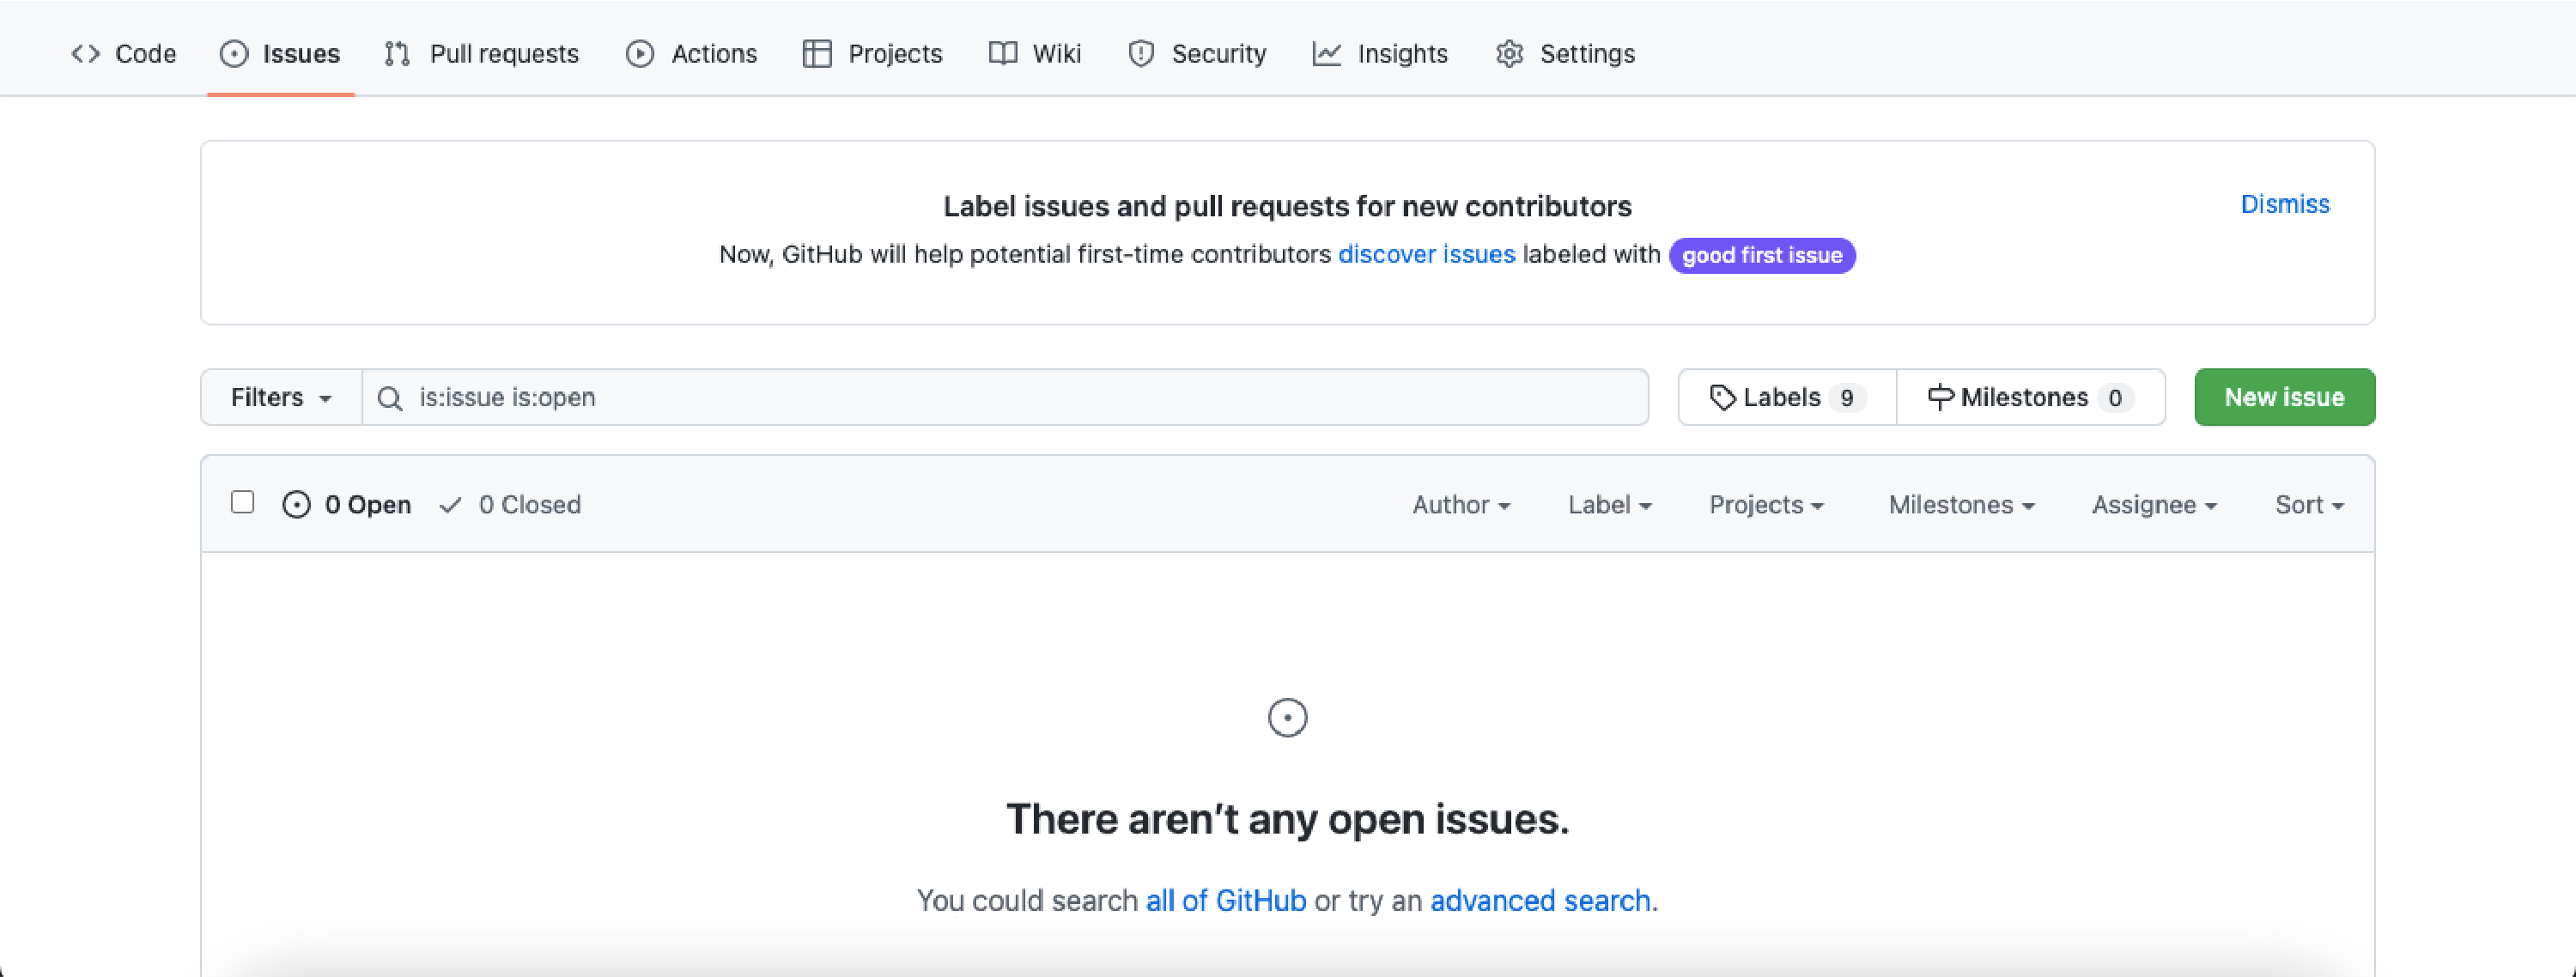
\includegraphics[width=\linewidth]{external/hub_issues_gs.pdf}
\end{image}%
\tcblower
\end{figureptx}%
\begin{figureptx}{Figure}{Example Issues page for the \href{https://github.com/scikit-learn/scikit-learn/issues}{Python module \mono{scikit-learn}}\protect\footnotemark{}}{figure-fig-hub-issues-skl}{}%
\begin{image}{0.05}{0.9}{0.05}{}%
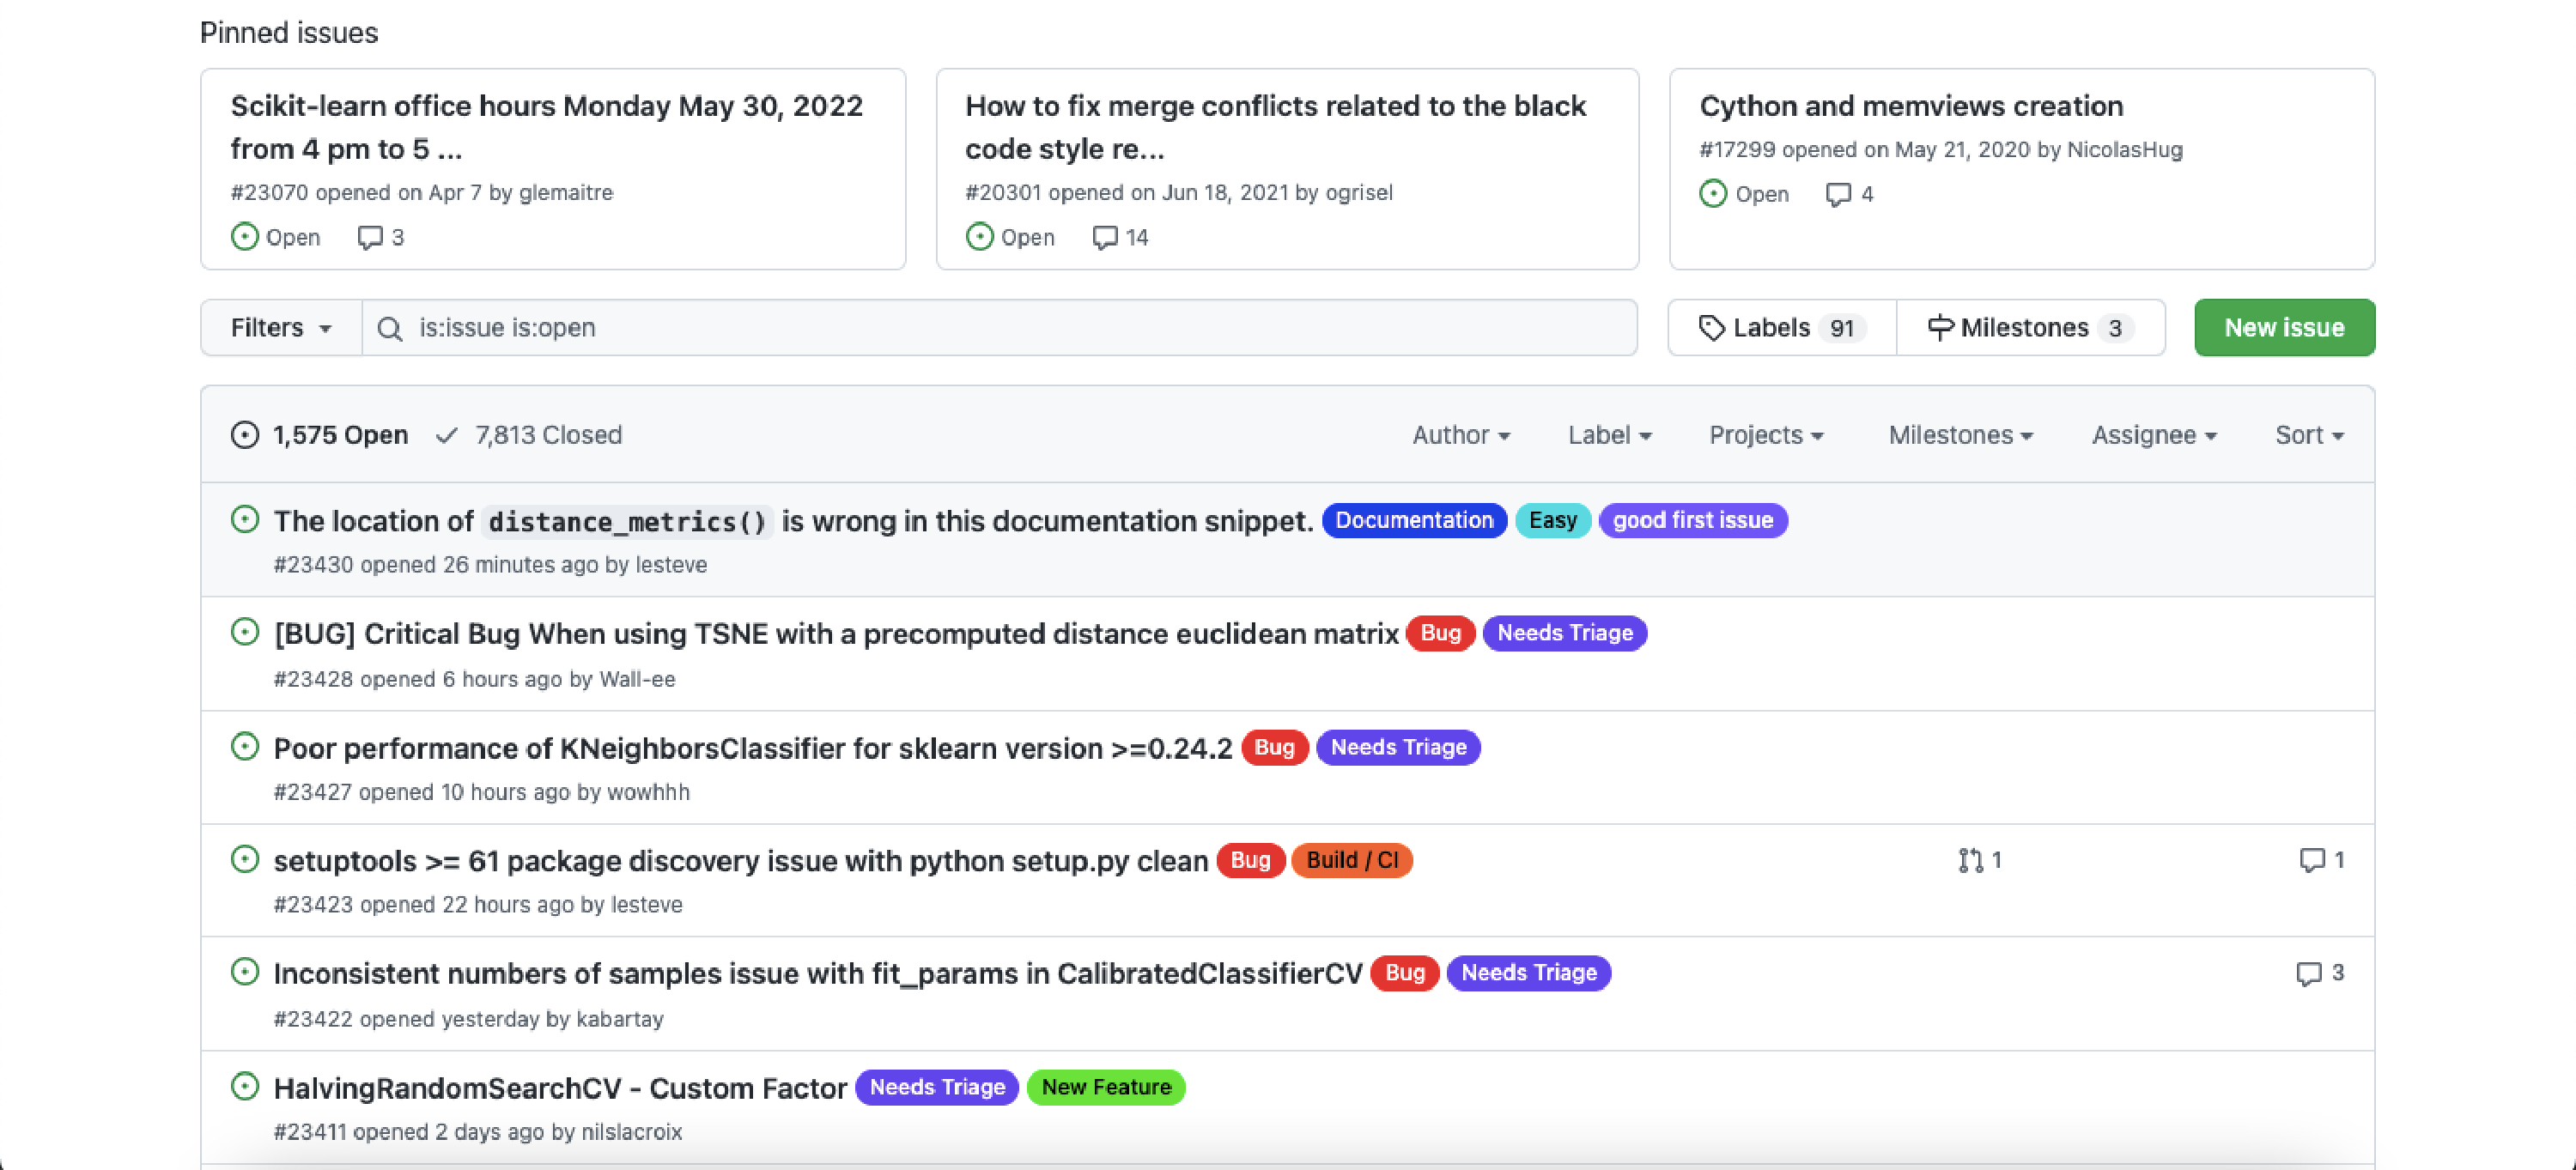
\includegraphics[width=\linewidth]{external/hub_issues_skl.pdf}
\end{image}%
\tcblower
\end{figureptx}%
\footnotetext[63]{\nolinkurl{github.com/scikit-learn/scikit-learn/issues}\label{fn-fig-hub-issues-skl-a-b}}%
\end{sectionptx}
%
%
\typeout{************************************************}
\typeout{Section B.2 Commit History}
\typeout{************************************************}
%
\begin{sectionptx}{Section}{Commit History}{}{Commit History}{}{}{section-S_hub-seecommits}
\index{commit history}%
\index{github!commit history}%
On the home page (Code tab) for all repositories a commit history can be found, full with contributor usernames, commit messages, and links to further information. Directly above the list of files, you can find information on the most recent commit. At the right side of this area is a clock icon with an arrow circling counterclockwise followed by a number of commits (See \hyperref[figure-fig-hub-ncommits]{Figure~{\xreffont\ref{figure-fig-hub-ncommits}}}). This is the total number of commits to that repository.%
\begin{figureptx}{Figure}{The number of commits to a repository}{figure-fig-hub-ncommits}{}%
\begin{image}{0.1}{0.8}{0.1}{}%
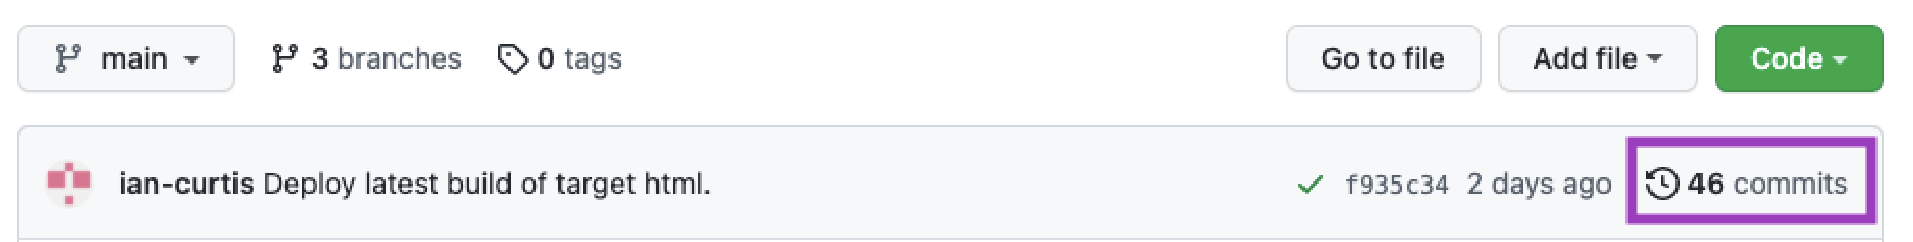
\includegraphics[width=\linewidth]{external/hub_ncommits.pdf}
\end{image}%
\tcblower
\end{figureptx}%
Clicking on this will give you more information on how often someone updates a repository and how many people do so. You are also able to see past branch names. Clicking on a specific commit will bring to a page with the files changed and any comments that were made.%
\par
Not everyone will be interested in this feature, but it is useful to know it is there should you want to take advantage of it.%
\end{sectionptx}
%
%
\typeout{************************************************}
\typeout{Section B.3 The About Panel}
\typeout{************************************************}
%
\begin{sectionptx}{Section}{The About Panel}{}{The About Panel}{}{}{section-S_hub-about}
\index{github!about panel}%
Most popular repositories have created and worked hard on their about panel. On any repo, this appears on the right side of the home page (Code tab) and it titled ``About''. This panel may include%
\begin{itemize}[label=\textbullet]
\item{}A short description%
\item{}A website%
\item{}Topics (these are like tags)%
\item{}A release version number%
\item{}Any packages published in the repository%
\item{}Any environments associated with the repository (such as GitHub Pages)%
\end{itemize}
%
\par
Also on this side of the page is a list of contributors, and the distribution of the langauges of the files in the repo (this can be off since GitHub doesn't recognize some file extensions). It's always nice to glance at this part of the page when looking at a repository just to get a general idea of what's going on or if it's what you are looking for. (A README will also help you understand more specific ideas about the repo content.)%
\end{sectionptx}
%
%
\typeout{************************************************}
\typeout{Section B.4 The Branch Tree Diagram (Network Graph)}
\typeout{************************************************}
%
\begin{sectionptx}{Section}{The Branch Tree Diagram (Network Graph)}{}{The Branch Tree Diagram (Network Graph)}{}{}{section-S_hubcollabtree}
\index{tree diagram}%
\index{github!tree diagram}%
\index{branches!tree diagram}%
\index{network graph|see{tree diagram}}%
Scattered throughout the book are various tree diagrams (created by me) depicting example branch pathways. Of course, these are highly variable depending on how many branches you have, commits you make, and contributors there are.%
\par
Turns out, GitHub actually makes a graph of your branches for you, as you create, push, merge, and delete them. This is visible on all public repos. To get to this graph, visit the Insights tab and then the Network page from the left sidebar. And there it is! It might not look very exciting, depending on your workflow. Consider the one for this book as of May 2022 in \hyperref[figure-fig-network-graph]{Figure~{\xreffont\ref{figure-fig-network-graph}}}.%
\begin{figureptx}{Figure}{Network graph for this book (as of May 2022)}{figure-fig-network-graph}{}%
\begin{image}{0.1}{0.8}{0.1}{}%
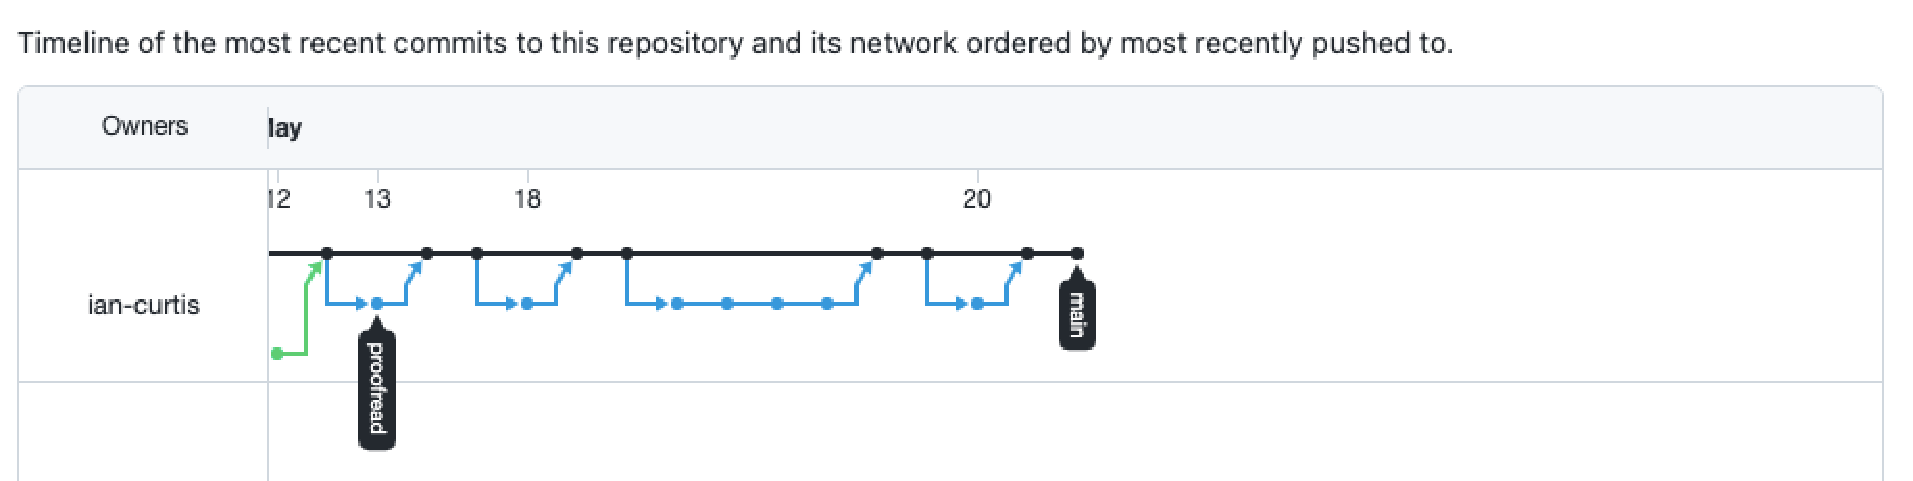
\includegraphics[width=\linewidth]{external/network_graph.pdf}
\end{image}%
\tcblower
\end{figureptx}%
\end{sectionptx}
%
%
\typeout{************************************************}
\typeout{Section B.5 Codespaces}
\typeout{************************************************}
%
\begin{sectionptx}{Section}{Codespaces}{}{Codespaces}{}{}{section-S_hub_codespace}
I personally prefer doing Git-related things on my personal computer (offline) and then updating GitHub when I'm ready. To me, it helps avoid unnecessary merge conflicts and make sure that my edits are only committed and pushed when I'm ready.%
\par
However, you don't have to work completely on your local computer. If you don't want to have all of this software downloaded (perhaps you're running out of storage space on your computer), there is another option: codespaces. This is \href{https://github.com/features/codespaces}{hosted by GitHub}\footnote{\nolinkurl{github.com/features/codespaces}\label{fn-S_hub_codespace-c-b}} and creates an online, virtual instance of your code files. By creating a codespace, you are using a virtual machine which runs the \initialism{VS} Code and is automatically connected to your GitHub repo. Codespaces could be useful if you need to edit something quickly and\slash{}or don't have access to your personal computer but make sure you create a branch before making a codespace.%
\par
If you choose to use this route, know that you are limited to 60 hours a month if you do not want to pay. You also should know that this is not available offline; an internet connection is required to work on a codespace.%
\par
So how do you make a codespace? It's easy!%
\begin{enumerate}
\item{}Head to the Code tab of your GitHub repository.%
\item{}Technically optional: create a branch. But I recommend you create a branch to lower the chance of conflicts.%
\item{}Click on the ``Code'' button (as if you were going to copy the HTTPS link for cloning).%
\item{}In the box that pops up, click on the Codespaces tab. In this tab is a button that says ``Create codespace on \textless{}branch-name\textgreater{}''. A codespace will generate (it may take some time) and should be ready to go as soon as it's done.%
\end{enumerate}
%
\end{sectionptx}
%
%
\typeout{************************************************}
\typeout{Section B.6 Deleting a Repository}
\typeout{************************************************}
%
\begin{sectionptx}{Section}{Deleting a Repository}{}{Deleting a Repository}{}{}{section-S_hub_delete_repo}
\index{repository!delete}%
\index{github!delete repository}%
So you really to delete a repository? Think long and hard about this one. Are you sure? Are you really sure? Deleting repos is \emph{irreversible} and can have lasting effects. For instance, all forks will be broken, but not deleted. If you delete a private repo, all forks will also be deleted. Any website that contains a link to your repo will no longer work and people might wonder where it went. And so on.%
\par
But here you are, so clearly you have decided to delete one. To delete a repository, you have to enter the danger zone (\pubtitle{Top Gun} anyone?).%
\begin{activity}{Activity}{Deleting a Repository.}{activity-hub-delete-repo}%
\begin{enumerate}[font=\bfseries,label=(\alph*),ref=\alph*]%
\item{}Navigate to the repo you want to delete.%
\item{}Click on the Settings tab. This should be the settings for the repo itself, not the general settings for your profile.%
\item{}Scroll all the way down to the Danger Zone.%
\item{}Click on ``Delete this repository''%
\item{}Read the dialog box that pops up. Once you have decided to delete the repo, type in what GitHub prompts you to type in and hit confirm.%
\end{enumerate}%
\end{activity}%
\end{sectionptx}
%
%
\typeout{************************************************}
\typeout{Section B.7 The \mono{.gitignore} File}
\typeout{************************************************}
%
\begin{sectionptx}{Section}{The \mono{.gitignore} File}{}{The \mono{.gitignore} File}{}{}{section-sec-hub-gitignore}
As you gain more experience with Git and GitHub, you may start wondering if there is a way to hide files from public view. Your project may come with files that are private to you\slash{}your company and are not necessary to share with everyone else. You also may have programs that generate files that are used by a second program and these intermediate files do not need to be shared. Whatever the circumstance, you can choose to block a file or folder from being tracked by Git.%
\par
The file for this is \mono{.gitignore}. The dot in front of the file name is necessary as this specifies that the file is, by default, ``hidden'' when being viewed in a file browser (to prevent accidentaly deletion). You should be able to edit this file on GitHub or access it with your text editor.%
\par
It is possible to generate a \mono{gitignore} template when creating a repo. These can be helpful but for my projects, I prefer to add the file manually and fill it in myself as I go.%
\par
All that goes in this file is a list of file\slash{}folder names and\slash{}or extensions you wish for Git to ignore. Keep one name per line. You can add comments to the file (to help break up sections) by starting a line with a hashtag (fine, a pound sign) and a space: \mono{\# This is a comment}. For example,%
\begin{codedisplay}
# Ignore generated images folder
generated-images/

# Random files to ignore
secret.txt
private_data.csv
\end{codedisplay}
%
\par
As a bonus, \mono{gitignore} files accept standard generalizing arguments and wildcards. For example, \mono{*.pdf} will ignore anything with the \mono{.pdf} file extension.%
\par
You should know that once Git tracks a file (or folder), you can't just add that file's name (or folder) to the \mono{gitignore} file and expect it to disappear. For any files you had Git tracking that you wish it would now ignore, see the instructions in \hyperref[section-S_untrackfiles]{Section~{\xreffont\ref{section-S_untrackfiles}}}. Note that any files you treat in this manner will still exist in the commit history of your repo and on any forks for your repo (the next time a user pulls changes from your repo, their copy of the file will be deleted). See \hyperref[warning-warn-untrack-delete]{Warning~{\xreffont\ref{warning-warn-untrack-delete}}}%
\end{sectionptx}
\end{appendixptx}
%
%
\typeout{************************************************}
\typeout{Appendix C Common Git Troubles and How To Fix Them}
\typeout{************************************************}
%
\begin{appendixptx}{Appendix}{Common Git Troubles and How To Fix Them}{}{Common Git Troubles and How To Fix Them}{}{}{appendix-app_gittroubles}
\renewcommand*{\appendixname}{Appendix}
\index{git!troubles}%
\begin{introduction}{}%
We all make mistakes, especially with Git. You don't know how many times I have staged the wrong files or committed my changes before realizing I did something wrong. Of course, it's best to try and avoid these issues becasue they can cause headaches and frustration. Plus there's usually a little fear involved (did I just erase my edits?) as well as hesitation (Git only does what I tell it, so I have to make sure I do it right). But just in case something happened that you didn't expect or you made a mistake, I have your back. Below are some common mistakes and questions you might ask.%
\end{introduction}%
%
%
\typeout{************************************************}
\typeout{Section C.1 Uh Oh, I Staged the Wrong Files!}
\typeout{************************************************}
%
\begin{sectionptx}{Section}{Uh Oh, I Staged the Wrong Files!}{}{Uh Oh, I Staged the Wrong Files!}{}{}{section-SS_reverseadd}
\index{git!add}%
\index{staging}%
Once you get the hang of Git, it's easy to just fly through the three-step process. In doing so, you will inevitably stage (with \mono{git add}) a file or folder on accident. This is relatively simple to fix. To undo this, follow the next procedure.%
\begin{project}{Git Procedure}{Reversing \mono{git add}.}{project-reverse-git-add}%
Oh shoot. What if you add a file you didn't mean to? This is one reason why there are so many steps to sending files to GitHub. Humans make mistakes and Git gives you the chance to correct any. Should you ever add a file you didn't mean to add, revist this procedure.%
\begin{enumerate}[font=\bfseries,label=(\alph*),ref=\alph*]%
\item{}Identify the file name(s) and extension(s) of the file(s) you mistakenly added.%
\item{}Use \mono{git restore --staged <your-file-name(s)>} to un-stage any files. Like \mono{git add}, this command can be run many times.%
\item{}It might be wise to verify with \mono{git status} that everything looks good.%
\end{enumerate}%
\end{project}%
\end{sectionptx}
%
%
\typeout{************************************************}
\typeout{Section C.2 Uh Oh, I Committed Too Early!}
\typeout{************************************************}
%
\begin{sectionptx}{Section}{Uh Oh, I Committed Too Early!}{}{Uh Oh, I Committed Too Early!}{}{}{section-SS_reversecommit}
\index{git!commit}%
\index{commit files}%
We've all been there. You \mono{add} all the files you need, double check to make sure you aren't missing anything, \mono{commit} with a message and suddenly remember a file you should have added. Never fear, \mono{git reset} is here!%
\begin{project}{Git Procedure}{Reversing \mono{git commit}.}{project-reverse-git-commit}%
\begin{enumerate}[font=\bfseries,label=(\alph*),ref=\alph*]%
\item{}You will only need this command: \mono{git reset --soft HEAD\textasciicircum{}1}. It should be safe to copy\slash{}paste this command directly into your command line and run it.%
\item{}\mono{git reset} gives no output so it is super important to check that the command worked with \mono{git status} (\hyperref[project-try-git-status]{Git Procedure~{\xreffont\ref{project-try-git-status}}}). If everything worked, you should see output as if you had used \mono{git status} after a \mono{git add} step.%
\par
Depending on how many commits you made, you may need to run this above command more than once. If so, make sure to use \mono{git status} after each try!%
\item{}Your previously staged files should still exist. From this point, use \mono{git add} to add your missing file(s) and proceed with \mono{git commit}.%
\end{enumerate}%
\end{project}%
\end{sectionptx}
%
%
\typeout{************************************************}
\typeout{Section C.3 Git Has Been Updating Files, But Now I Don't Want It To}
\typeout{************************************************}
%
\begin{sectionptx}{Section}{Git Has Been Updating Files, But Now I Don't Want It To}{}{Git Has Been Updating Files, But Now I Don't Want It To}{}{}{section-S_untrackfiles}
\index{tracking}%
\index{git!tracking}%
This is actually pretty common. Maybe you are writing a book and your abandoned chapters were on GitHub for your editors to look at. Now that the book is published, you don't want those chapters online. Maybe you are using an API and when you were developing a project had your app's API connection keys available and not that the project is public you want to remove the file containing them.%
\par
When Git is keeping track of files, we say that it is \terminology{tracking} files. Untracking files is not super difficult, but does, like all Git commands, require the command line.%
\begin{warning}{Warning}{}{warning-warn-untrack-delete}%
Untracking files from Git \emph{does not delete them from your local computer}. However, the next time you push to GitHub, they will no longer be there. Thus, the next time your collaborators pull from the repository, their copy of the file will be deleted.%
\end{warning}
\begin{project}{Git Procedure}{Untracking Files from Git.}{project-S_untrackfiles-g}%
\begin{enumerate}[font=\bfseries,label=(\alph*),ref=\alph*]%
\item{}Identify the \emph{files} you wish to remove from Git's tracking service%
\item{}Use \mono{git rm --cached <filename>}. You may also add multiple files as done with \mono{git add} (\hyperref[project-try-git-add]{Git Procedure~{\xreffont\ref{project-try-git-add}}}).%
\item{}Want to untrack folders? You will need the \mono{-r} recursive option. So, \mono{git rm -r --cached <folder-name>} will do the trick.%
\item{}The above options will not delete the file(s)\slash{}folder(s) from your local computer. If you would like the files deleted and untracked, use the above commands with out the \mono{--cached} feature: \mono{git rm <filenames>} and \mono{git rm -r <folder-names>}.%
\end{enumerate}%
\end{project}%
\end{sectionptx}
%
%
\typeout{************************************************}
\typeout{Section C.4 Git Won't Let Me Pull From Upstream or Origin!}
\typeout{************************************************}
%
\begin{sectionptx}{Section}{Git Won't Let Me Pull From Upstream or Origin!}{}{Git Won't Let Me Pull From Upstream or Origin!}{}{}{section-S_forcemerge}
\index{git!pull}%
\index{remote!upstream}%
\index{remote!origin}%
\index{upstream}%
\index{origin}%
\begin{introduction}{}%
Ah, perhaps you forgot to make a branch. This error happens to me a lot when I have a lot of work on the main branch because I never made a separate branch (not smart of me, I know).%
\par
Or maybe not. Either way, Git says you have a problem with your code and won't let you merge from upstream. Maybe you get a message like this:%
\begin{console}{0}{1}{0}
> (*\consoleinput{git pull upstream main}*)
error: Your local changes to the following files would be overwritten by merge:
        <file-name(s)>
Please commit your changes or stash them before you merge.
Aborting
\end{console}
This error occurs when you have local, uncommitted changes and a merge from origin or upstream has changes in the same exact places. Git has no idea whose changes to keep so it does nothing. There are a couple of different things you can do in this situation depending on how you feel about your changes.%
\end{introduction}%
%
%
\typeout{************************************************}
\typeout{Subsection C.4.1 Your Local Changes Are Irrelevant and You Want Them Overwritten}
\typeout{************************************************}
%
\begin{subsectionptx}{Subsection}{Your Local Changes Are Irrelevant and You Want Them Overwritten}{}{Your Local Changes Are Irrelevant and You Want Them Overwritten}{}{}{subsection-S_forcemerge-h}
\index{force merge}%
This definitely happens! Perhaps you tried a few things and they didn't work so you want to pull from upstream or origin and start over. Maybe you corrected some typos and someone else beat you to it so you want to merge their corrections in and keep working. I could go on and on. It's not difficult at all to force Git to make this happen, just make sure this is what you want to do!%
\begin{project}{Git Procedure}{Forcing an Upstream or Origin Merge.}{project-S_forcemerge-h-d}%
\begin{enumerate}[font=\bfseries,label=(\alph*),ref=\alph*]%
\item{}First, create a backup branch just in case things go haywire: \mono{git branch backup}. Since \mono{git branch} does not automatically switch you to that branch, you are free to carry on.%
\item{}Now, just fetch the changes. Remember that merging and fetching are separate processes. Fetching just collects the changes, attempting to merge will throw the error. Use \mono{git fetch <remote> <branch-name>}. Example: \mono{git fetch upstream main}.%
\item{}Now reset your current branch to the contents you just fetched. This is not a merge, this is a complete reset. You are reverting all of your content to match what you just fetched. This is why we created a backup in case something gets deleted that you didn't want to be.%
\par
In the event that a file you created gets deleted from the reset, just navigate to the backup branch, stage just the missing file and commit just the missing file to origin. Then pull from origin.%
\par
But to reset, use \mono{git reset --hard <remote>/<branch-name>}. Continuing the example from above, \mono{git reset --hard upstream/main}%
\end{enumerate}%
\end{project}%
\end{subsectionptx}
%
%
\typeout{************************************************}
\typeout{Subsection C.4.2 Your Local Changes are Good and You Want to Keep Them}
\typeout{************************************************}
%
\begin{subsectionptx}{Subsection}{Your Local Changes are Good and You Want to Keep Them}{}{Your Local Changes are Good and You Want to Keep Them}{}{}{subsection-S_forcemerge-i}
\index{git!stash}%
\index{stash}%
Sometimes your changes are valid and you want them to be kept, but you still want to pull in changes. One option is to force a merge conflict and deal with it in your editor, choosing which version to keep. If this is what you want to do, just \mono{add} the troublesome files, \mono{commit} them, then \mono{pull}. Again, this will force a merge conflict but you can fix things from there.%
\par
Alternatively, you can keep your changes by using \mono{git stash}. Stashing will store your changes locally without committing and will let you pull. To bring your changes back you can use \mono{git stash pop}. In my experience, things have worked out quite nicely with \mono{git stash}. I just type \mono{git stash} before pulling, then I pull, then I use \mono{git stash pop} and my changes are popped right back into where they were. For more information, you might find \href{https://opensource.com/article/21/4/git-stash}{opensource.com}\footnote{\nolinkurl{opensource.com/article/21/4/git-stash}\label{fn-S_forcemerge-i-e-g}} useful.%
\par
If \mono{git stash pop} doesn't work, you may have a bigger problem on your hands. You will want to do a Google search if this is your case. This happened to me at one point and unfortunately I had to completely reset my local repository to what was appearing on GitHub. In such an extreme case, I even made a copy of some of my files with my edits before doing any resetting so I could easily add my changes back in.%
\end{subsectionptx}
\end{sectionptx}
%
%
\typeout{************************************************}
\typeout{Section C.5 Git Says I Have Divergent Branches!}
\typeout{************************************************}
%
\begin{sectionptx}{Section}{Git Says I Have Divergent Branches!}{}{Git Says I Have Divergent Branches!}{}{}{section-S_diverge_branch}
I recently experienced this issue for the first time and had to do some searching to figure out how to fix it. I relied on \href{https://stackoverflow.com/questions/62653114}{Davide Casiraghi's question on StackOverflow}\footnote{\nolinkurl{https://stackoverflow.com/questions/62653114}\label{fn-S_diverge_branch-b-b}} and \href{https://stackoverflow.com/questions/29673869/}{adrianvlupu's question also on StackOverflow}\footnote{\nolinkurl{https://stackoverflow.com/questions/29673869/}\label{fn-S_diverge_branch-b-d}} to create this guide and you might find these resources more helpful than mine.%
\par
This is a preemptive warning of a merge conflict and occurs when you are trying to pull in or push out a commit and another commit gets in the way. Git doesn't want to create them, so it refuses to push or pull until you fix something. This is not the same error as in \hyperref[section-S_forcemerge]{Section~{\xreffont\ref{section-S_forcemerge}}}, although it is closely related. You might get something like this:%
\begin{console}{0}{1}{0}
> (*\consoleinput{git push}*)
To <repo-you-are-pushing-to>.git
 ! [rejected]        main -> main (fetch first)
error: failed to push some refs to '<repo-you-are-pushing-to>.git'
hint: Updates were rejected because the remote contains work that you do
hint: not have locally. This is usually caused by another repository pushing
hint: to the same ref. You may want to first integrate the remote changes
hint: (e.g., 'git pull ...') before pushing again.
hint: See the 'Note about fast-forwards' in 'git push --help' for details.
\end{console}
This looks kind of scary. Let's see how to fix this.%
\begin{project}{Git Procedure}{Consolidating Divergent Branches.}{project-try-git-rebase}%
\begin{enumerate}[font=\bfseries,label=(\alph*),ref=\alph*]%
\item{}The first step will be to try to pull in changes before you push. Use \mono{git pull <remote> <branch>} as needed. If this works, then try to push and everything should be ok.%
\par
You might get another error like this:%
\begin{console}{0}{1}{0}
> (*\consoleinput{git pull origin main}*)
remote: Enumerating objects: 1, done.
remote: Counting objects: 100% (1/1), done.
remote: Total 1 (delta 0), reused 0 (delta 0), pack-reused 0
Unpacking objects: 100% (1/1), 659 bytes | 659.00 KiB/s, done.
From <repo-you-are-pushing-to>
   2417195..8b492ee  main       -> origin/main
hint: You have divergent branches and need to specify how to reconcile them.
hint: You can do so by running one of the following commands sometime before
hint: your next pull:
hint: 
hint:   git config pull.rebase false  # merge
hint:   git config pull.rebase true   # rebase
hint:   git config pull.ff only       # fast-forward only
hint: 
hint: You can replace "git config" with "git config --global" to set a default
hint: preference for all repositories. You can also pass --rebase, --no-rebase,
hint: or --ff-only on the command line to override the configured default per
hint: invocation.
fatal: Need to specify how to reconcile divergent branches.
\end{console}
which is quite overwhelming.%
\item{}Here, the fix is usually pretty easy but I have to teach you a new term. We need to \terminology{rebase} the branch. When a pull happens, Git fetches new commits from GitHub and merges them into your branch (and this merge is actually a commit in itself). The rebase command will temporarily remove your new commits from the commit history, then pull in the new changes and reinstate your commit into the timeline.%
\par
If you want to avoid potential large error messages like this again, you might consider changing Git's default behavior. Instead of fetching and merging, you can do a fast-forward merge which does not do a merge commit. When a fast forward is not possible, the error message is much shorter and then you can use the rebase command to fix things.%
\par
To begin this process, first enter \mono{git config pull.ff only} into your terminal. This will change the default pull behavior for Git (for your current repository only).%
\item{}Now try \mono{git pull}. Things might work. Great! But if you get an error message of \mono{fatal: Not possible to fast-forward, aborting.}, use \mono{git pull --rebase} to perform a rebase. Then \mono{git push} back to origin or upstream.%
\par
If you ever want to change the default behavior back to what it was, use \mono{git config pull.rebase false}. If you want to keep that behavior change we just did and you want to do a one-time fetch-merge pull (the old way), use \mono{git pull --ff}.%
\end{enumerate}%
\end{project}%
\end{sectionptx}
%
%
\typeout{************************************************}
\typeout{Section C.6 Reverting To a Previous Commit}
\typeout{************************************************}
%
\begin{sectionptx}{Section}{Reverting To a Previous Commit}{}{Reverting To a Previous Commit}{}{}{section-S_hub_revert_commit}
\index{commit!revert}%
\index{revert commit}%
\index{git!commit}%
\index{commit hash}%
\index{commit!hash}%
I have never had to do this (yet) so I don't have direct experience here. However, \href{https://gist.github.com/gunjanpatel/18f9e4d1eb609597c50c2118e416e6a6}{user gunjanpatel on GitHub}\footnote{\nolinkurl{gist.github.com/gunjanpatel/18f9e4d1eb609597c50c2118e416e6a6}\label{fn-S_hub_revert_commit-g-b}} has created a nice guide. It appears that \mono{git reset HEAD\textasciicircum{} --hard} and then \mono{git push origin -f} will work. The \mono{-f} switch forces the push and ignores errors.%
\par
Some of the guide above refers to what is known as a \terminology{commit hash}, a unique string that identifies each commit on GitHub. These are actually so unique that we only need the first few characters of the string to identify the commit. You can find the hash by using \hyperref[section-S_hub-seecommits]{Section~{\xreffont\ref{section-S_hub-seecommits}}}. The string is the random numbers\slash{}letters found on the right side of each commit.%
\end{sectionptx}
%
%
\typeout{************************************************}
\typeout{Section C.7 Merge Conflicts}
\typeout{************************************************}
%
\begin{sectionptx}{Section}{Merge Conflicts}{}{Merge Conflicts}{}{}{section-S_mergeconflict}
Hopefully you never have to deal with these. Sometimes, they are pretty simple to fix. Other times, it can cause some headaches. To avoid merge conflicts, pull from upstream often (\hyperref[warning-warn-fetch-often]{Warning~{\xreffont\ref{warning-warn-fetch-often}}} and \hyperref[warning-warn-pull-often]{Warning~{\xreffont\ref{warning-warn-pull-often}}}). Merge conflicts are caused when more than one person edits the same line of a file. It is possible for two people to edit the same file, but on different lines, and not cause a conflict.%
\par
I have never caused or had to deal with a serious merge conflict. \href{https://docs.github.com/en/pull-requests/collaborating-with-pull-requests/addressing-merge-conflicts/resolving-a-merge-conflict-on-github}{The GitHub documentation}\footnote{\nolinkurl{docs.github.com/en/pull-requests/collaborating-with-pull-requests/addressing-merge-conflicts/resolving-a-merge-conflict-on-github}\label{fn-S_mergeconflict-c-b}} has a good post on how to resolve conflicts on GitHub. GitHub will even show you the two (or more) versions and let you choose how to resolve them. You can also \href{https://docs.github.com/en/pull-requests/collaborating-with-pull-requests/addressing-merge-conflicts/resolving-a-merge-conflict-using-the-command-line}{resolve merge conflicts on the command line}\footnote{\nolinkurl{docs.github.com/en/pull-requests/collaborating-with-pull-requests/addressing-merge-conflicts/resolving-a-merge-conflict-using-the-command-line}\label{fn-S_mergeconflict-c-d}} or in your text editor.%
\par
I have accidentally caused a merge conflict with myself and with working on the same repository from two different computers and two different accounts. Oops! This is an easy fix because I made the conflict with myself so I know which version is the correct one. If this happens to you, Git might send you to an unfamiliar screen when you try to push or pull. You'll know you have this case if your terminal asks you to type in a reason why the merge must happen or how the conflict is resolved. This typically happens when you try to merge from an upstream main into a local main that has active changes (so create branches!).%
\par
If you start to get stuck, do a quick Google search. There are many guides and resources out there to help with merge conflicts. \href{https://happygitwithr.com/git-branches.html?q=merge\%20confli\#dealing-with-conflicts}{Jennifer Bryan}\footnote{\nolinkurl{https://happygitwithr.com/git-branches.html?q=merge\%20confli\#dealing-with-conflicts}\label{fn-S_mergeconflict-e-b}} has a good guide on merge conflict basics (and some other potential Git issues!) so start there and explore more as needed.%
\begin{project}{Git Procedure}{Merging from main to main (remote contains changes not on local).}{project-S_mergeconflict-f}%
This is for when you are sent into a command line editing tool or a default text editor asking you to provide a reason why the merge is necessary. This may not solve your problem but sometimes all a merge conflict needs is to bypass this screen.%
\begin{enumerate}[font=\bfseries,label=(\alph*),ref=\alph*]%
\item{}Type \mono{i}%
\item{}Type a merge message. This can be something as simple as ``I have to merge to move on'' or ``I know what I want, let me do it'' (yes, I have actually put that as a message\textellipsis{}is this good? Who knows?).%
\item{}Press \kbd{esc}.%
\item{}Type \mono{:wq} (this stands for write and quit)%
\item{}Press \kbd{Enter} and you may be ok to move forward with the pushing, pulling, and creating of pull requests.%
\end{enumerate}%
\end{project}%
\end{sectionptx}
\end{appendixptx}
%
%
\typeout{************************************************}
\typeout{Appendix D Common Commands}
\typeout{************************************************}
%
\begin{appendixptx}{Appendix}{Common Commands}{}{Common Commands}{}{}{appendix-app-git-commands}
\renewcommand*{\appendixname}{Appendix}
\begin{introduction}{}%
Need a little help remembering all of the commands discussed in this book? Look no further! Use this page as a cheat sheet to help you keep track of the common commands used here (you will also likely use these often in your future endeavors).%
\end{introduction}%
%
%
\typeout{************************************************}
\typeout{Section D.1 General Commands}
\typeout{************************************************}
%
\begin{sectionptx}{Section}{General Commands}{}{General Commands}{}{}{section-common-commands}
Here you find a list of commands that can be used at the command line anywhere (and aren't necessarily associated with Git).%
\begin{descriptionlist}
\begin{dlimedium}{\mono{pwd}}{li-common-commands-b-a-a}%
Used to find the present working directory (i.e.\@, the current active folder).%
\end{dlimedium}%
\begin{dlimedium}{\mono{cd}}{li-common-commands-b-a-b}%
Used to change the active directory (folder) in the terminal. Requires either the file path to move into or \mono{..} to move backwards one level.%
\end{dlimedium}%
\begin{dlimedium}{\mono{ls}}{li-common-commands-b-a-c}%
Used to list the contents of the active folder.%
\end{dlimedium}%
\begin{dlimedium}{\mono{touch}}{li-common-commands-b-a-d}%
Used to create files. Also requires the filename and file extension of the file you wish to create.%
\end{dlimedium}%
\begin{dlimedium}{\mono{open} (or \mono{start})}{li-common-commands-b-a-e}%
Used to open a file, folder, or application using the defualt application\slash{}service%
\end{dlimedium}%
\begin{dlimedium}{\mono{killall} (Mac only)}{li-common-commands-b-a-f}%
Used to close an entire application%
\end{dlimedium}%
\begin{dlimedium}{\mono{mkdir}}{li-common-commands-b-a-g}%
Used to create a new folder. Also requires the name of the folder to create.%
\end{dlimedium}%
\begin{dlimedium}{\mono{rm}}{li-common-commands-b-a-h}%
Used to remove a file (without warnings). Also requires the file name and extension you want to remove.%
\end{dlimedium}%
\begin{dlimedium}{\mono{rmdir}}{li-common-commands-b-a-i}%
Used to remove a folder (without warnings). Also requires the folder name to remove.%
\end{dlimedium}%
\begin{dlimedium}{\mono{clear}}{li-common-commands-b-a-j}%
Used to clear the terminal screen and bring the cursor back to the top of the window.%
\end{dlimedium}%
\begin{dlimedium}{\mono{code}}{li-common-commands-b-a-k}%
Used to open files or folders with the application \initialism{VS} Code.%
\end{dlimedium}%
\end{descriptionlist}
%
\end{sectionptx}
%
%
\typeout{************************************************}
\typeout{Section D.2 Git Commands}
\typeout{************************************************}
%
\begin{sectionptx}{Section}{Git Commands}{}{Git Commands}{}{}{section-git-commands}
This section contains the most common commands used at the command line to interact with Git. To see these commands in the context of a workflow, see \hyperref[section-S_gitsumm]{Section~{\xreffont\ref{section-S_gitsumm}}} and \hyperref[section-S_gitcollabsumm]{Section~{\xreffont\ref{section-S_gitcollabsumm}}}.%
\begin{descriptionlist}
\begin{dlimedium}{\mono{git clone}}{li-git-commands-b-c-a}%
Used to copy (``clone'') a repository from GitHub to a local source. Also requires an HTTPS link copied from GitHub.%
\end{dlimedium}%
\begin{dlimedium}{\mono{git branch}}{li-git-commands-b-c-b}%
Used to create a new branch in the background. Also requires the name of the branch you wish to create.%
\end{dlimedium}%
\begin{dlimedium}{\mono{git switch}}{li-git-commands-b-c-c}%
Used to change branches. Also requires the branch name you wish to change to.%
\par
Can be used as \mono{git switch -c} with a branch name to create and change to a branch automatically (i.e.\@, \mono{git branch} is not required).%
\end{dlimedium}%
\begin{dlimedium}{\mono{git status}}{li-git-commands-b-c-d}%
Used to check up on the state of Git operations. Can be entered at any time in the Git process.%
\end{dlimedium}%
\begin{dlimedium}{\mono{git add}}{li-git-commands-b-c-e}%
Used to stage files to prepare them for committing and attaching a commit message. Requires either a \mono{.} (to add all modified\slash{}new files) or a number of file and folder names.%
\end{dlimedium}%
\begin{dlimedium}{\mono{git commit -m}}{li-git-commands-b-c-f}%
Used to commit files and to attach a commit message (surrounded in quotes). Automatically attaches this message to the files staged using \mono{git add} and makes a stamp in the respective file timelines.%
\end{dlimedium}%
\begin{dlimedium}{\mono{git push}}{li-git-commands-b-c-g}%
Used to push changes from a local source to GitHub. Requires the remote repository (\mono{origin} or \mono{upstream}) and the branch name you wish to send changes to.%
\end{dlimedium}%
\begin{dlimedium}{\mono{git pull}}{li-git-commands-b-c-h}%
Used to pull in changes from GitHub to a local repository. Requires the remote repository (\mono{origin} or \mono{upstream}) and the branch name you wish to pull changes from.%
\end{dlimedium}%
\end{descriptionlist}
%
\end{sectionptx}
\end{appendixptx}
%
%
\typeout{************************************************}
\typeout{Appendix E Answers to All Activities and Exercises}
\typeout{************************************************}
%
\begin{solutions-chapter}{Appendix}{Answers to All Activities and Exercises}{}{Answers to All Activities and Exercises}{}{}{solutions-app_answers}
\par\medskip
\noindent\textbf{\Large{}I\space\textperiodcentered\space{}Introductory Information\\
1\space\textperiodcentered\space{}Computer Basics\\
1.1\space\textperiodcentered\space{}File and Folder Names\\
1.1.2\space\textperiodcentered\space{}Exploring File and Folder Naming Techniques}
\begin{activitysolution}{Activity}{1.1}{Folder Naming.}{activity-taylorswiftfolders}%
\begin{enumerate}[font=\bfseries,label=(\alph*),ref=\alph*]%
\item[(a)]\noindent\textbf{\blocktitlefont Solution}.\hypertarget{solution-taylorswiftfolders-d-b-back}{}\quad{}The main thing that pops out to me are the spaces. Every multi-word folder name has a space. Secondly, some of the names are very long. Third, there is not much consistency. Some names are capitalized, others aren't. There are clearly deluxe versions of albums but some say ``deluxe'', others say ``deluxe version'', and even others say ``deluxe edition''.%
\par
The three here are the main issues; you may have thought of others. Great! I'm sure they are good observations.%
\item[(b)]\noindent\textbf{\blocktitlefont Solution}.\hypertarget{solution-taylorswiftgroups-b-back}{}\quad{}There are probably a lot of patterns you could have noticed. I grouped folder names into%
\begin{enumerate}[label=\arabic*]
\item{}Standard albums%
\item{}Deluxe albums%
\item{}Live albums%
\item{}Taylor's Version albums%
\item{}Other%
\end{enumerate}
%
\item[(c)]\noindent\textbf{\blocktitlefont Solution}.\hypertarget{solution-taylorswiftfolders-f-b-back}{}\quad{}Since there aren't any special modifiers to this album (such as deluxe or live), I say we just keep its name, but write them in kebab-case. Therefore, ``Taylor Swift'' would become \mono{taylor-swift}.%
\item[(d)]\noindent\textbf{\blocktitlefont Solution}.\hypertarget{solution-taylorswiftfolders-g-b-back}{}\quad{}The following names are the modified versions:%
\begin{multicols}{2}
\begin{itemize}[label=\textbullet]
\item{}\mono{taylor-swift}%
\item{}\mono{fearless}%
\item{}\mono{speak-now}%
\item{}\mono{red}%
\item{}\mono{1989}%
\item{}\mono{reputation}%
\item{}\mono{lover}%
\item{}\mono{folklore}%
\item{}\mono{evermore}%
\item{}\mono{midnights}%
\end{itemize}
\end{multicols}
%
\item[(e)]\noindent\textbf{\blocktitlefont Solution}.\hypertarget{solution-taylorswiftfolders-h-b-back}{}\quad{}For the deluxe albums, the similarity is the word ``deluxe''. I don't bother with ``edition'' or ``version'', ``deluxe'' is enough to convey the necessary information. I also would like to abbreviate ``deluxe'' to ``dlx''. You could also choose to keep the full word, but since we can't ask Taylor what she would prefer, I am sticking with the shorter. ``dlx'' gets the point across (this is a deluxe album) with 3 less characters. Following are my changes for the deluxe group. There is one outlier: the Fearless Platinum Edition. I am going to retain the ``platinum'' name since that is its true name.%
\begin{multicols}{2}
\begin{itemize}[label=\textbullet]
\item{}\mono{taylor-swift-dlx}%
\item{}\mono{fearless-pltnm}%
\item{}\mono{speak-now-dlx}%
\item{}\mono{red-dlx}%
\item{}\mono{1989-dlx}%
\item{}\mono{folklore-dlx}%
\item{}\mono{folklore-dsny-dlx}%
\item{}\mono{evermore-dlx}%
\item{}\mono{midnights-dlx-3am}%
\item{}\mono{midnights-dlx-dawn}%
\end{itemize}
\end{multicols}
%
\item[(f)]\noindent\textbf{\blocktitlefont Solution}.\hypertarget{solution-taylorswiftfolders-i-b-back}{}\quad{}There are only two in this group, but there could be more in the future. Let's use ``live'' to differentiate these folders from the others. I am choosing to not use ``lve'' or ``lv'' because I think there are slightly ambiguous (it could mean ``love''!).%
\begin{itemize}[label=\textbullet]
\item{}\mono{clear-chnl-live}%
\item{}\mono{speak-now-live}%
\end{itemize}
%
\item[(g)]\noindent\textbf{\blocktitlefont Solution}.\hypertarget{solution-taylorswiftfolders-j-b-back}{}\quad{}I am going to again use kebab-case and use ``tv'' to indicate that the album is a Taylor's Version. This will help cut down on name length.%
\begin{itemize}[label=\textbullet]
\item{}\mono{fearless-tv}%
\item{}\mono{red-tv}%
\item{}\mono{speak-now-tv}%
\end{itemize}
%
\item[(h)]\noindent\textbf{\blocktitlefont Solution}.\hypertarget{solution-taylorswiftfolders-k-b-back}{}\quad{}These are mostly up to you. They have no specific pattern, but I will still apply kebab-case and shorten the names.%
\begin{itemize}[label=\textbullet]
\item{}\mono{holiday-clctn} (I could even use \mono{holiday} since there is only one holiday album)%
\item{}\mono{unreleased}%
\item{}\mono{singles}%
\end{itemize}
%
\end{enumerate}%
\end{activitysolution}%
\begin{activitysolution}{Activity}{1.2}{File Naming.}{activity-taylorswiftfiles}%
\begin{enumerate}[font=\bfseries,label=(\alph*),ref=\alph*]%
\item[(a)]\noindent\textbf{\blocktitlefont Solution}.\hypertarget{solution-taylorswiftfiles-d-b-back}{}\quad{}The main thing that pops out to me are the spaces. Every multi-word file name has a space. Secondly, there are a few cases of non-consistency: Back To December says ``Acoustic'' whereas Haunted says ``Acoustic Version''.%
\par
The two here are the main issues; you may have thought of others. Great! I'm sure they are good observations.%
\item[(b)]\noindent\textbf{\blocktitlefont Solution}.\hypertarget{solution-taylorswiftgroups2-b-back}{}\quad{}There are probably a couple patterns you could have noticed. I grouped track names into%
\begin{enumerate}[label=\arabic*]
\item{}``Regular'' album tracks%
\item{}Acoustic tracks%
\item{}The last track%
\end{enumerate}
%
\item[(c)]\noindent\textbf{\blocktitlefont Solution}.\hypertarget{solution-taylorswiftfiles-f-b-back}{}\quad{}There isn't much we can do here. I will write the names in snake\textunderscore{}case which will remove the spaces and change every word to lowercase. Since we can't ask Taylor for her preferences, it is up to you whether you want to abbreviate words or not. For the most part, I do not since most track names are short already.%
\begin{multicols}{2}
\begin{itemize}[label=\textbullet]
\item{}\mono{01\_mine.wav}%
\item{}\mono{02\_sparks\_fly.wav}%
\item{}\mono{03\_back\_to\_dec.wav}%
\item{}\mono{04\_speak\_now.wav}%
\item{}\mono{05\_dear\_john.wav}%
\item{}\mono{06\_mean.wav}%
\item{}\mono{07\_story\_of\_us.wav}%
\item{}\mono{08\_never\_grow\_up.wav}%
\item{}\mono{09\_enchanted.wav}%
\item{}\mono{10\_better\_than\_revenge.wav}%
\item{}\mono{11\_innocent.wav}%
\item{}\mono{12\_haunted.wav}%
\item{}\mono{13\_last\_kiss.wav}%
\item{}\mono{14\_long\_live.wav}%
\item{}\mono{15\_ours.wav}%
\item{}\mono{16\_if\_this\_was\_movie.wav}%
\item{}\mono{17\_superman.wav}%
\end{itemize}
\end{multicols}
%
\item[(d)]\noindent\textbf{\blocktitlefont Solution}.\hypertarget{solution-taylorswiftfiles-g-b-back}{}\quad{}I am choosing to abbreviate ``acoustic'' to ``acoust''. Notice I used the same names as the regular tracks, but just appended ``\textunderscore{}acoust'' at the end.%
\begin{itemize}[label=\textbullet]
\item{}\mono{18\_back\_to\_dec\_acoust.wav}%
\item{}\mono{19\_haunted\_acoust.wav}%
\end{itemize}
%
\item[(e)]\noindent\textbf{\blocktitlefont Solution}.\hypertarget{solution-taylorswiftfiles-h-b-back}{}\quad{}I am choosing to abbreviate ``POP Mix'' to ``pop\textunderscore{}mix''. Notice I used the same name as the regular tracks, but just appended ``\textunderscore{}pop\textunderscore{}mix'' at the end.%
\begin{itemize}[label=\textbullet]
\item{}\mono{20\_mine\_pop\_mix.wav}%
\end{itemize}
%
\end{enumerate}%
\end{activitysolution}%
\par\medskip
\noindent\textbf{\Large{}2\space\textperiodcentered\space{}The Command Line\\
2.3\space\textperiodcentered\space{}Basic Commands\\
2.3.2\space\textperiodcentered\space{}Navigating Your Computer With the Command Line}
\begin{inlinesolution}{Checkpoint}{2.3.2.3}{Trying \mono{cd}.}{exercise-try-cd}%
\par\smallskip%
\noindent\textbf{\blocktitlefont Hint}.\hypertarget{hint-try-cd-c-back}{}\quad{}Try running \mono{pwd} after \mono{cd}. Do you notice anything different here?%
\end{inlinesolution}%
\par\medskip
\noindent\textbf{\Large{}2.3.3\space\textperiodcentered\space{}Adding Files and Directories}
\begin{activitysolution}{Activity}{2.1}{File Extensions Matter.}{activity-fileextensions}%
\begin{enumerate}[font=\bfseries,label=(\alph*),ref=\alph*]%
\item[(c)]\noindent\textbf{\blocktitlefont Answer}.\hypertarget{answer-fileextensions-g-b-back}{}\quad{}Mac users likely see the TextEdit app open. This is the default app for opening files like this. Windows users will be prompted to determine which application should be used to open the file.%
\end{enumerate}%
\end{activitysolution}%
\begin{inlinesolution}{Checkpoint}{2.3.3.2}{Trying \mono{open}.}{exercise-try-open}%
\par\smallskip%
\noindent\textbf{\blocktitlefont Answer}.\hypertarget{answer-try-open-c-back}{}\quad{}\mono{open test.txt} or \mono{start text.txt}%
\end{inlinesolution}%
\begin{inlinesolution}{Checkpoint}{2.3.3.3}{Trying \mono{killall}.}{exercise-try-killall}%
\par\smallskip%
\noindent\textbf{\blocktitlefont Solution}.\hypertarget{solution-try-killall-c-back}{}\quad{}Your computer should have opened up TextEdit (the default text editor for Mac) when attempting to open the previous file. To close this application, you should enter \mono{killall TextEdit} at the command line.%
\end{inlinesolution}%
\begin{activitysolution}{Activity}{2.2}{Putting It All Together, Part 1.}{activity-trycdtouch}%
\begin{enumerate}[font=\bfseries,label=(\alph*),ref=\alph*]%
\item[(a)]\noindent\textbf{\blocktitlefont Answer}.\hypertarget{answer-trycdtouch-d-b-back}{}\quad{}\mono{cd testdir} should do the trick!%
\item[(b)]\noindent\textbf{\blocktitlefont Answer}.\hypertarget{answer-trycdtouch-e-b-back}{}\quad{}Use \mono{ls} and \mono{pwd} here.%
\par\smallskip%
\noindent\textbf{\blocktitlefont Solution}.\hypertarget{solution-trycdtouch-e-c-back}{}\quad{}Since we just created this directory, \mono{ls} should not show any files; no output should be provided. \mono{pwd} can be used to find the file path which should look like%
\begin{codedisplay}
/Users/<your-username>/Desktop/testdir
\end{codedisplay}
or%
\begin{codedisplay}
/c/Users/<your-username>/Desktop/testdir
\end{codedisplay}
%
\item[(c)]\noindent\textbf{\blocktitlefont Hint}.\hypertarget{hint-trycdtouch-f-b-back}{}\quad{}You can use \mono{ls} to verify that everything worked.%
\par\smallskip%
\noindent\textbf{\blocktitlefont Answer}.\hypertarget{answer-trycdtouch-f-c-back}{}\quad{}\mono{touch my\_greeting.txt} OR \mono{touch myGreeting.txt} OR \mono{touch my-greeting.txt} OR \mono{MyGreeting.txt} OR \mono{MY\_GREETING.txt}%
\par\smallskip%
\noindent\textbf{\blocktitlefont Solution}.\hypertarget{solution-trycdtouch-f-d-back}{}\quad{}Whenever we create a new file (of any type), we use \mono{touch}. Recall that \mono{touch} requires three pieces: the command, the file name, and the file extension. The command is \mono{touch}, the file name is \mono{my\_greeting} (recommended, although there are other possible names), and the file extension is \mono{.txt}. Put these together, and we get \mono{touch my\_greeting.txt}.%
\item[(d)]\noindent\textbf{\blocktitlefont Answer}.\hypertarget{answer-trycdtouch-g-b-back}{}\quad{}\mono{open my\_greeting.txt} OR \mono{open <file-name>.txt}%
\item[(e)]\noindent\textbf{\blocktitlefont Answer}.\hypertarget{answer-trycdtouch-h-b-back}{}\quad{}This is a \mono{.txt} file: \mono{killall TextEdit}.%
\end{enumerate}%
\end{activitysolution}%
\par\medskip
\noindent\textbf{\Large{}2.3.4\space\textperiodcentered\space{}Removing Files and Directories}
\begin{inlinesolution}{Checkpoint}{2.3.4.1}{Trying \mono{rm}.}{exercise-try-rm}%
\begin{enumerate}[font=\bfseries,label=(\alph*),ref=\alph*]%
\item[(b)]\noindent\textbf{\blocktitlefont Answer}.\hypertarget{answer-try-rm-c-b-back}{}\quad{}\mono{rm my\_greeting.txt}%
\end{enumerate}%
\end{inlinesolution}%
\begin{inlinesolution}{Checkpoint}{2.3.4.3}{Trying \mono{cd} Backwards.}{exercise-try-cd-backwards}%
\par\smallskip%
\noindent\textbf{\blocktitlefont Hint}.\hypertarget{hint-try-cd-backwards-c-back}{}\quad{}If successful, \mono{pwd} should indicate that you are in the Desktop.%
\par\smallskip%
\noindent\textbf{\blocktitlefont Answer}.\hypertarget{answer-try-cd-backwards-d-back}{}\quad{}\mono{cd ..}%
\par\smallskip%
\noindent\textbf{\blocktitlefont Solution}.\hypertarget{solution-try-cd-backwards-e-back}{}\quad{}As mentioned, \mono{cd ..} will move you backwards. If you run \mono{pwd}, you should see that you have returned to the Desktop; \mono{ls} should give you all of the files we were working with before.%
\end{inlinesolution}%
\begin{inlinesolution}{Checkpoint}{2.3.4.4}{Trying \mono{rmdir}.}{exercise-try-rmdir}%
\par\smallskip%
\noindent\textbf{\blocktitlefont Answer}.\hypertarget{answer-try-rmdir-c-back}{}\quad{}\mono{rmdir testdir}%
\end{inlinesolution}%
\begin{activitysolution}{Activity}{2.3}{Putting It All Together, Part 2.}{activity-try-removing}%
\begin{enumerate}[font=\bfseries,label=(\alph*),ref=\alph*]%
\item[(a)]\noindent\textbf{\blocktitlefont Answer}.\hypertarget{answer-try-removing-d-b-back}{}\quad{}Use \mono{pwd} to check if still on Desktop, \mono{rm <file-name>} to remove files, and \mono{ls} to check if the files are gone.%
\item[(b)]\noindent\textbf{\blocktitlefont Answer}.\hypertarget{answer-try-removing-e-b-back}{}\quad{}\mono{cd ..}%
\item[(c)]\noindent\textbf{\blocktitlefont Answer}.\hypertarget{answer-try-removing-f-b-back}{}\quad{}\mono{cd Documents} OR \mono{mkdir Documents}, then \mono{cd Documents}%
\item[(d)]\noindent\textbf{\blocktitlefont Answer}.\hypertarget{answer-try-removing-g-b-back}{}\quad{}\mono{mkdir my-favorites} (could use a different case)%
\item[(e)]\noindent\textbf{\blocktitlefont Answer}.\hypertarget{answer-try-removing-h-b-back}{}\quad{}\mono{cd my\_favorites}, \mono{pwd}%
\item[(f)]\noindent\textbf{\blocktitlefont Answer}.\hypertarget{answer-try-removing-i-b-back}{}\quad{}\mono{touch food.txt}, \mono{touch hobbies.docx}, \mono{touch smells.xslx}; \mono{ls}%
\item[(g)]\noindent\textbf{\blocktitlefont Answer}.\hypertarget{answer-try-removing-j-b-back}{}\quad{}Mac: \mono{open food.txt}, \mono{killall TextEdit}; \mono{open hobbies.docx}, \mono{killall \textquotesingle{}Microsoft Word\textquotesingle{}}, \mono{open smells.xslx}, \mono{killall \textquotesingle{}Microsoft Excel\textquotesingle{}}%
\par
Windows: \mono{start food.txt}, \mono{start hobbies.docx}, \mono{start smells.xslx}%
\item[(h)]\noindent\textbf{\blocktitlefont Answer}.\hypertarget{answer-try-removing-k-b-back}{}\quad{}\mono{rm food.txt}, \mono{rm hobbies.docx}, \mono{rm smells.xslx}; \mono{ls}%
\item[(i)]\noindent\textbf{\blocktitlefont Answer}.\hypertarget{answer-try-removing-l-b-back}{}\quad{}\mono{cd ..}, \mono{pwd}%
\item[(j)]\noindent\textbf{\blocktitlefont Answer}.\hypertarget{answer-try-removing-m-b-back}{}\quad{}\mono{rmdir my-favorites}, \mono{ls}%
\end{enumerate}%
\end{activitysolution}%
\par\medskip
\noindent\textbf{\Large{}II\space\textperiodcentered\space{}Working Solo\\
3\space\textperiodcentered\space{}GitHub Solo\\
3.2\space\textperiodcentered\space{}The First Repository and File\\
3.2.3\space\textperiodcentered\space{}Editing a File}
\begin{inlinesolution}{Checkpoint}{3.2.3.4}{}{exercise-try-markdown}%
\begin{enumerate}[font=\bfseries,label=(\alph*),ref=\alph*]%
\item[(g)]\noindent\textbf{\blocktitlefont Hint}.\hypertarget{hint-try-markdown-i-b-back}{}\quad{}To add images, you will need to make sure you specify the correct filepath to the image. This can be hard to get right as it depends on where the image is saved and where your Markdown file lives on your computer. If the image doesn't appear at first, you might try making sure the image and the Markdown file are in the same folder and seeing if things work out better.%
\end{enumerate}%
\end{inlinesolution}%
\par\medskip
\noindent\textbf{\Large{}4\space\textperiodcentered\space{}Git Solo\\
4.3\space\textperiodcentered\space{}Sending Changes Back To GitHub: The Three-Step Process\\
4.3.1\space\textperiodcentered\space{}Wait, Which Files Did I Change Again?}
\begin{projectsolution}{Git Procedure}{4.4}{Trying \mono{git status}.}{project-try-git-status}%
\par\smallskip%
\noindent\textbf{\blocktitlefont Solution}.\hypertarget{solution-try-git-status-e-back}{}\quad{}You might see a console output such as the one below.%
\begin{console}{0}{1}{0}
> (*\consoleinput{git status}*)
On branch country
Changes not staged for commit:
  (use "git add <file>..." to update what will be committed)
  (use "git restore <file>..." to discard changes in working directory)
        modified:   README.md

no changes added to commit (use "git add" and/or "git commit -a")
\end{console}
We get a lot more information than needed right now, but we will break this output down shortly. For now, notice that we get a statement of the branch we are on and a file name that represents a file we have modified. It is not recreated here, but the modified file name is red in the output (any new, untracked files will be green).%
\end{projectsolution}%
\par\medskip
\noindent\textbf{\Large{}4.3.2\space\textperiodcentered\space{}Step 1: Staging Files}
\begin{projectsolution}{Git Procedure}{4.5}{Trying \mono{git add}.}{project-try-git-add}%
\begin{enumerate}[font=\bfseries,label=(\alph*),ref=\alph*]%
\item[(b)]\noindent\textbf{\blocktitlefont Hint}.\hypertarget{hint-try-git-add-d-b-back}{}\quad{}Case 1 or Case 3 will work in this instance.%
\par\smallskip%
\noindent\textbf{\blocktitlefont Answer}.\hypertarget{answer-try-git-add-d-c-back}{}\quad{}\mono{git add README.md} OR \mono{git add .}. Neither will produce any output.%
\item[(c)]\noindent\textbf{\blocktitlefont Answer}.\hypertarget{answer-try-git-add-e-b-back}{}\quad{}\begin{console}{0}{1}{0}
> (*\consoleinput{git status}*)
On branch country
Changes to be committed:
  (use "git restore --staged <file>..." to unstage)
        modified:   README.md
\end{console}
The text color has changed to green which indicates the process worked.%
\end{enumerate}%
\end{projectsolution}%
\par\medskip
\noindent\textbf{\Large{}4.3.3\space\textperiodcentered\space{}Step 2: Committing Files}
\begin{projectsolution}{Git Procedure}{4.6}{Trying \mono{git commit}.}{project-try-git-commit}%
\begin{enumerate}[font=\bfseries,label=(\alph*),ref=\alph*]%
\item[(c)]\noindent\textbf{\blocktitlefont Answer}.\hypertarget{answer-try-git-commit-e-b-back}{}\quad{}\begin{console}{0}{1}{0}
> (*\consoleinput{git status}*)
On branch country
nothing to commit, working tree clean
\end{console}
This output is what is to be expected! Don't fret that it says nothing to commit. This is completely true since we just finished committing everything that we had staged. This output means that everything worked correctly.%
\end{enumerate}%
\end{projectsolution}%
\par\medskip
\noindent\textbf{\Large{}4.3.4\space\textperiodcentered\space{}Step 3: Pushing Files}
\begin{projectsolution}{Git Procedure}{4.7}{Trying \mono{git push}.}{project-try-git-push}%
\begin{enumerate}[font=\bfseries,label=(\alph*),ref=\alph*]%
\item[(a)]\begin{enumerate}[font=\bfseries,label=(\roman*),ref=\theenumi.\roman*]%
\item[(i)]\noindent\textbf{\blocktitlefont Solution}.\hypertarget{solution-try-git-push-c-b-b-back}{}\quad{}\begin{console}{0}{1}{0}
> (*\consoleinput{git push}*)
fatal: The current branch country has no upstream branch.
To push the current branch and set the remote as upstream, use

    git push --set-upstream origin country
\end{console}
Well that looks a little scary. Fatal! That just means that git wansn't able to complete your request and stopped trying. The reason this failed is because the branch \mono{country} is only on your computer, it hasn't yet made it to GitHub (which is what we are trying to do). It is possible to create a remote connection between branches but I often don't especially if I am only working on one branch at a time and if I plan on deleting a branch when I'm done with it. Should you want to create a remote, use the command Git provided.%
\item[(ii)]\noindent\textbf{\blocktitlefont Solution}.\hypertarget{solution-try-git-push-c-c-b-back}{}\quad{}\begin{console}{0}{1}{0}
> (*\consoleinput{git push origin}*)
fatal: The current branch country has no upstream branch.
To push the current branch and set the remote as upstream, use

    git push --set-upstream origin country
\end{console}
Well, look at that, the same error. This should make sense. You are telling Git to push changes to the origin repo but \mono{country}, the current branch, doesn't have an origin since we created the branch locally.%
\item[(iii)]\noindent\textbf{\blocktitlefont Solution}.\hypertarget{solution-try-git-push-c-d-b-back}{}\quad{}\begin{console}{0}{1}{0}
> (*\consoleinput{git push country}*)
fatal: 'country' does not appear to be a git repository
fatal: Could not read from remote repository.

Please make sure you have the correct access rights
and the repository exists.
\end{console}
Remember the four parts to \mono{git push}? Well since we forgot Step 3, the remote name, Git assumes that the word ``country'' is the name of the repo we want to push to. Since there is no repo named ``country'' on your computer nor on GitHub, it doens't know where to push and errors out.%
\end{enumerate}%
\item[(b)]\begin{enumerate}[font=\bfseries,label=(\roman*),ref=\theenumi.\roman*]%
\item[(i)]\noindent\textbf{\blocktitlefont Answer}.\hypertarget{answer-try-git-push-d-b-b-back}{}\quad{}Here, to follow with the example, we will use \mono{origin} and the branch name \mono{country}.%
\item[(ii)]\noindent\textbf{\blocktitlefont Solution}.\hypertarget{solution-try-git-push-d-c-b-back}{}\quad{}\begin{console}{0}{1}{0}
> (*\consoleinput{git push origin country}*)
Enumerating objects: 5, done.
Counting objects: 100% (5/5), done.
Delta compression using up to 4 threads
Compressing objects: 100% (2/2), done.
Writing objects: 100% (3/3), 330 bytes | 82.00 KiB/s, done.
Total 3 (delta 1), reused 0 (delta 0), pack-reused 0
remote: Resolving deltas: 100% (1/1), completed with 1 local object.
remote: 
remote: Create a pull request for 'country' on GitHub by visiting:
remote:      <url-to-pull-request>
remote: 
To <url-to-origin-repo>
 * [new branch]      country -> country
\end{console}
We get a lot of output for a successful push. Most of it is just information that can be useful in certain cases and might be worth a glance to make sure things worked as expected.%
\end{enumerate}%
\end{enumerate}%
\end{projectsolution}%
\par\medskip
\noindent\textbf{\Large{}4.4\space\textperiodcentered\space{}The Final Steps}
\begin{projectsolution}{Git Procedure}{4.10}{Trying \mono{git pull}.}{project-try-git-pull}%
\begin{enumerate}[font=\bfseries,label=(\alph*),ref=\alph*]%
\item[(b)]\noindent\textbf{\blocktitlefont Answer}.\hypertarget{answer-try-git-pull-f-b-back}{}\quad{}\mono{git switch main}%
\item[(c)]\noindent\textbf{\blocktitlefont Answer}.\hypertarget{answer-try-git-pull-g-b-back}{}\quad{}\begin{console}{0}{1}{0}
> (*\consoleinput{git pull origin main}*)
remote: Enumerating objects: 1, done.
remote: Counting objects: 100% (1/1), done.
remote: Total 1 (delta 0), reused 0 (delta 0), pack-reused 0
Unpacking objects: 100% (1/1), 631 bytes | 631.00 KiB/s, done.
From <repo-url>
   <commit-id>  main       -> origin/main
Updating <commit-id>
Fast-forward
 README.md | 4 ++++
 1 file changed, 4 insertions(+)
\end{console}
\end{enumerate}%
\end{projectsolution}%
\par\medskip
\noindent\textbf{\Large{}4.6\space\textperiodcentered\space{}Working Solo: The Culminating Experience}
\begin{activitysolution}{Activity}{4.11}{}{activity-git-big-act}%
\begin{enumerate}[font=\bfseries,label=(\alph*),ref=\alph*]%
\item[(a)]\noindent\textbf{\blocktitlefont Answer}.\hypertarget{answer-git-ba-newrepo-b-back}{}\quad{}Use one of the multiple methods to create a new repo in GitHub. Perhaps name it \mono{poems} or \mono{fav-poems}? This part is up to you as long as the name accurately describes the future repo contents. Check the box that says to add a README file.%
\item[(b)]\noindent\textbf{\blocktitlefont Hint}.\hypertarget{hint-git-ba-clone-b-back}{}\quad{}Make sure you are not ``inside'' your previous repositories. Nested repositories will not work. So \mono{cd} to the folder in which you want to place your new repo.%
\par\smallskip%
\noindent\textbf{\blocktitlefont Answer}.\hypertarget{answer-git-ba-clone-c-back}{}\quad{}Copy the HTTPS link on GitHub. Use \mono{git clone <copied-link>}. Use \mono{cd <repo-name>} to move your terminal into that repo.%
\item[(c)]\noindent\textbf{\blocktitlefont Answer}.\hypertarget{answer-git-big-act-d-b-back}{}\quad{}\mono{git branch readme} then \mono{git switch readme} OR \mono{git switch -c readme}%
\par
You may use any branch name you like as long as it's clear what the branch is for. ``readme'' seems like it will work nicely.%
\item[(d)]\noindent\textbf{\blocktitlefont Answer}.\hypertarget{answer-git-big-act-e-b-back}{}\quad{}Perhaps a better title would be ``My Favorite Poems'' or ``Two Original Poems''. This can vary. You might explain that this repository contains two of your favorite poems (or two poems you wrote yourself) and this it was born from a project in \pubtitle{Better Git Started} to help you get more familiar with GitHub and Git functions. This can also vary.%
\item[(e)]\noindent\textbf{\blocktitlefont Answer}.\hypertarget{answer-git-big-act-f-b-back}{}\quad{}\mono{git status}%
\item[(f)]\noindent\textbf{\blocktitlefont Answer}.\hypertarget{answer-git-big-act-g-b-back}{}\quad{}\mono{git add .} OR \mono{git add README.md}, maybe \mono{git status} to confirm?%
\item[(g)]\noindent\textbf{\blocktitlefont Answer}.\hypertarget{answer-git-big-act-h-b-back}{}\quad{}\mono{git commit -m \textquotesingle{}edit readme with repo info\textquotesingle{}}, maybe \mono{git status} to confirm?%
\par
Of course, your commit message may be different. Perhaps ``edit readme'' and enough for you.%
\item[(h)]\noindent\textbf{\blocktitlefont Answer}.\hypertarget{answer-git-big-act-i-b-back}{}\quad{}\mono{git push origin <your-branch-name>}%
\item[(i)]\noindent\textbf{\blocktitlefont Answer}.\hypertarget{answer-git-big-act-j-b-back}{}\quad{}``Compare and pull request'', ``Merge'', ``Confirm merge''. (Check the main branch on GitHub to make sure this worked.)%
\item[(j)]\noindent\textbf{\blocktitlefont Answer}.\hypertarget{answer-git-big-act-k-b-back}{}\quad{}\mono{git switch main} then \mono{git pull origin main}%
\item[(k)]\noindent\textbf{\blocktitlefont Answer}.\hypertarget{answer-git-big-act-l-b-back}{}\quad{}\mono{git branch poems} then \mono{git switch poems} OR \mono{git switch -c poems}%
\par
You may use any branch name you like as long as it's clear what the branch is for. ``poems'' works for me.%
\par
Note that you could split up each poem into its own branch. Depending on the length of your poems, you may want to do that in practice but here we will edit both on one branch. That way you can practice two commits in one push!%
\item[(l)]\noindent\textbf{\blocktitlefont Hint}.\hypertarget{hint-git-big-act-m-b-back}{}\quad{}In \initialism{VS} Code, you can create a new file with the paper-with-a-plus icon in the ``Explorer'' panel in the top left.%
\par\smallskip%
\noindent\textbf{\blocktitlefont Answer}.\hypertarget{answer-git-big-act-m-c-back}{}\quad{}Use the hint or use your terminal (\mono{touch poem1.md}).%
\item[(n)]\noindent\textbf{\blocktitlefont Answer}.\hypertarget{answer-git-big-act-o-b-back}{}\quad{}\mono{git add .} OR \mono{git add poem1.md}, then \mono{git status}%
\par
Your text editor might also indicate that this worked. For instance, \initialism{VS} Code will show an ``A'' next to the file name.%
\item[(o)]\noindent\textbf{\blocktitlefont Answer}.\hypertarget{answer-git-big-act-p-b-back}{}\quad{}\mono{git commit -m \textquotedbl{}<commit-message>\textquotedbl{}}, \mono{git status}%
\par
Your text editor might also indicate that this worked. For instance, \initialism{VS} Code will remove and letters and colors next to the file name. It will also show your commit message in the ``Timeline'' panel on the bottom left.%
\item[(p)]\noindent\textbf{\blocktitlefont Answer}.\hypertarget{answer-git-big-act-q-b-back}{}\quad{}After editing, \mono{git add .} or \mono{git add poem2.md}. Then \mono{git commit -m \textquotedbl{}<message>\textquotedbl{}}. \mono{git status} might be useful here.%
\item[(q)]\noindent\textbf{\blocktitlefont Answer}.\hypertarget{answer-git-big-act-r-b-back}{}\quad{}\mono{git push origin <branch-name>}, ``Compare and pull request'', ``Merge'', ``Confirm merge''.%
\item[(r)]\noindent\textbf{\blocktitlefont Answer}.\hypertarget{answer-git-big-act-s-b-back}{}\quad{}\mono{git switch main}, then \mono{git pull origin main}%
\end{enumerate}%
\end{activitysolution}%
\par\medskip
\noindent\textbf{\Large{}III\space\textperiodcentered\space{}Working With Others\\
6\space\textperiodcentered\space{}Git Collaboration\\
6.1\space\textperiodcentered\space{}Getting Set Up: A Few Extra Steps\\
6.1.1\space\textperiodcentered\space{}Cloning A Fork}
\begin{inlinesolution}{Checkpoint}{6.1.1.1}{}{exercise-SS_gitcollabclone-f}%
\noindent\textbf{\blocktitlefont Solution}.\hypertarget{solution-SS_gitcollabclone-f-b-back}{}\quad{}Use the code tab \emph{on your fork} to copy the \initialism{HTTPS} link. Then use \mono{git clone <https-link>}. Make sure you have used \mono{cd} to get to the right place first!%
\end{inlinesolution}%
\par\medskip
\noindent\textbf{\Large{}6.1.2\space\textperiodcentered\space{}Don't Forget About Branches!}
\begin{inlinesolution}{Checkpoint}{6.1.2.1}{}{exercise-SS_gitcollabbranch-g}%
\noindent\textbf{\blocktitlefont Solution}.\hypertarget{solution-SS_gitcollabbranch-g-b-back}{}\quad{}There are a couple of choices here.%
\begin{enumerate}
\item{}\mono{git branch <name>} then \mono{git switch <name>}%
\item{}\mono{git switch -c <name>}%
\end{enumerate}
%
\end{inlinesolution}%
\par\medskip
\noindent\textbf{\Large{}6.4\space\textperiodcentered\space{}The Final Steps\\
6.4.2\space\textperiodcentered\space{}Pulling\slash{}Fetching Upstream}
\begin{projectsolution}{Git Procedure}{6.1}{Updating Origin and Local, Method 1.}{project-try-git-pull-origin}%
\begin{enumerate}[font=\bfseries,label=(\alph*),ref=\alph*]%
\item[(c)]\noindent\textbf{\blocktitlefont Answer}.\hypertarget{answer-try-git-pull-origin-i-b-back}{}\quad{}\mono{git pull origin main} (if you are pulling from origin, just \mono{git pull} can work, too)%
\end{enumerate}%
\end{projectsolution}%
\par\medskip
\noindent\textbf{\Large{}6.6\space\textperiodcentered\space{}Working Together: The Culminating Experience}
\begin{activitysolution}{Activity}{6.3}{}{activity-bigact-gitcollab}%
\begin{enumerate}[font=\bfseries,label=(\alph*),ref=\alph*]%
\item[(b)]\noindent\textbf{\blocktitlefont Answer}.\hypertarget{answer-bigact-gitcollab-c-b-back}{}\quad{}Click on the ``Fork'' button in the top right. (You can keep the same name.)%
\item[(d)]\noindent\textbf{\blocktitlefont Answer}.\hypertarget{answer-bigact-gitcollab-e-b-back}{}\quad{}Copy the \initialism{HTTPS} link \emph{to your fork} on GitHub. Use \mono{git clone <copied-link>}. Use \mono{cd <repo-name>} to move your terminal into that repo.%
\item[(e)]\noindent\textbf{\blocktitlefont Answer}.\hypertarget{answer-bigact-gitcollab-f-b-back}{}\quad{}This could vary. Perhaps \mono{superpower}, \mono{power}, or \mono{add-superpower}?%
\item[(f)]\noindent\textbf{\blocktitlefont Answer}.\hypertarget{answer-bigact-gitcollab-g-b-back}{}\quad{}\mono{cd book-activities} first, then \mono{code superpower.md} to open just the markdown file (not the entire repository) (if using \initialism{VS} Code); if using a different editor, use Google to find a good terminal command (or do it manually)%
\par
OR \mono{cd ..} to go backwards a folder, then \mono{code gitstarted} to open the entire repository, then open the markdown file using work (to use Git functions again, you may have to \mono{cd gitstarted} again)%
\item[(h)]\noindent\textbf{\blocktitlefont Answer}.\hypertarget{answer-bigact-gitcollab-i-b-back}{}\quad{}\mono{git status}%
\item[(i)]\noindent\textbf{\blocktitlefont Answer}.\hypertarget{answer-bigact-gitcollab-j-b-back}{}\quad{}%
\begin{itemize}[label=\textbullet]
\item{}\mono{git add .} or%
\item{}\mono{git add book-activities/} or%
\item{}\mono{git add book-activities/superpower.md}%
\end{itemize}
%
\item[(j)]\noindent\textbf{\blocktitlefont Answer}.\hypertarget{answer-bigact-gitcollab-k-b-back}{}\quad{}\mono{git status}%
\item[(k)]\noindent\textbf{\blocktitlefont Answer}.\hypertarget{answer-bigact-gitcollab-l-b-back}{}\quad{}\mono{git commit -m \textquotesingle{}<your-message>\textquotesingle{}}%
\item[(l)]\noindent\textbf{\blocktitlefont Answer}.\hypertarget{answer-bigact-gitcollab-m-b-back}{}\quad{}\mono{git push origin superpower}%
\item[(m)]\noindent\textbf{\blocktitlefont Answer}.\hypertarget{answer-bigact-gitcollab-n-b-back}{}\quad{}Create a pull reqeust from \mono{superpower} to your fork's \mono{main} then from your fork's \mono{main} to upstream \mono{main}.%
\par
OR Create a pull request from \mono{superpower} directly to the upstream \mono{main}.%
\item[(o)]\noindent\textbf{\blocktitlefont Answer}.\hypertarget{answer-bigact-gitcollab-p-b-back}{}\quad{}\mono{git switch main}, then%
\par
\mono{git remote add upstream https://github.com/ian-curtis/gitstarted.git}%
\par
It is important to switch back to main or you will set an upstream remote for just your branch which is sometimes useful, but not here.%
\item[(p)]\noindent\textbf{\blocktitlefont Answer}.\hypertarget{answer-bigact-gitcollab-q-b-back}{}\quad{}(on main branch) \mono{git pull upstream main}, \mono{git push origin main}%
\end{enumerate}%
\end{activitysolution}%
\end{solutions-chapter}
%
\backmatter%
%
\clearpage\phantomsection%
\addcontentsline{toc}{part}{Back Matter}%
%
%% The index is here, setup is all in preamble
%% Index locators are cross-references, so same font here
{\xreffont\printindex}
%
\clearpage
\pagestyle{empty}
\vspace*{\stretch{1}}
\begin{backcolophon}{Colophon}{colophon-backmatter-h}%
This book was authored in PreTeXt.%
\end{backcolophon}%
\vspace*{\stretch{2}}
\end{document}
